% generated from JIRA project LVV
% using template at /usr/share/miniconda/envs/docsteady-env/lib/python3.7/site-packages/docsteady/templates/tpr.latex.jinja2.
% using docsteady version 2.3.0
% Please do not edit -- update information in Jira instead
\documentclass[SE,,STR,toc]{lsstdoc}
\usepackage{geometry}
\usepackage{longtable,booktabs}
\usepackage{enumitem}
\usepackage{arydshln}
\usepackage{attachfile}
\usepackage{array}
\usepackage{dashrule}

\newcolumntype{L}[1]{>{\raggedright\let\newline\\\arraybackslash\hspace{0pt}}p{#1}}

\input meta.tex

\newcommand{\attachmentsUrl}{https://github.com/\gitorg/\lsstDocType-\lsstDocNum/blob/\gitref/attachments}
\providecommand{\tightlist}{
  \setlength{\itemsep}{0pt}\setlength{\parskip}{0pt}}

\setcounter{tocdepth}{4}

\begin{document}

\def\milestoneName{Hexapod Actuator Redesign Verification}
\def\milestoneId{}
\def\product{Hexapod and Rotator}

\setDocCompact{true}

\title{LVV-P95: Hexapod Actuator Redesign Verification Test Plan and Report}
\setDocRef{\lsstDocType-\lsstDocNum}
\date{ 2023-04-10 }
\author{ Kevin Siruno }

% Most recent last
\setDocChangeRecord{
\addtohist{}{2023-02-27}{First draft}{M.Lutfi, K.Siruno}
}

\setDocCurator{M.Lutfi, K.Siruno}
\setDocUpstreamLocation{\url{https://github.com/lsst-dm/\lsstDocType-\lsstDocNum}}
\setDocUpstreamVersion{\vcsRevision}



\setDocAbstract{
This is the test plan and report for
\textbf{ Hexapod Actuator Redesign Verification},
an LSST milestone pertaining to the Data Management Subsystem.\\
This document is based on content automatically extracted from the Jira test database on \docDate.
The most recent change to the document repository was on \vcsDate.
}


\maketitle

\section{Introduction}
\label{sect:intro}


\subsection{Objectives}
\label{sect:objectives}

 The objective of this test plan is to verify the Hexapods requirements
will still be met after changing the design of the encoders on the
hexapod actuators. In order to do this, a series of tests will be
conducted on a single actuator first and then a subset of these tests
will be repeated with the remaining actuators. Once all of the actuators
have been verified, there will be a final verification event for the
entire hexapod.



\subsection{System Overview}
\label{sect:systemoverview}

 \begin{itemize}
\item
  Both the M2 Cell Assembly and Camera use hexapods to facilitate rigid
  body optical positioning relative to the M1M3 Mirror. These hexapods
  utilize identical actuators to facilitate ease of maintainability and
  interchangeability.Actuators incorporate a rotary motor, harmonic
  drive, and a screw. An absolute linear encoder measures the actuator
  length and a relative rotary encoder measures the motor rotation;
  smooth, stiction free flexures provide end rotations; software limits
  electrical limit switches, and hard stops limit travel. Each Actuator
  weighs \textasciitilde{}58.8 kg and measures 620 mm in length.~
\item
  Due to various issues/damages, linear encoders of the hexapod
  actuators will need repair/service/replacement.~

  \begin{itemize}
  \item
    Replacing/servicing the encoder head or tape requires disassembly
    the actuators.
  \item
    Disassembling an actuator requires removing it from the hexapod.
  \item
    Removing the hexapod requires first removing the payload, either the
    camera or M2 mirror cell assembly. ~ ~ ~~
  \end{itemize}
\item
  Hence, all actuators will adopt a modified design to facilitate in
  situ servicing of the linear encoder.
\end{itemize}


\subsection{Document Overview}
\label{sect:docoverview}

This document was generated from Jira, obtaining the relevant information from the
\href{https://jira.lsstcorp.org/secure/Tests.jspa\#/testPlan/LVV-P95}{LVV-P95}
~Jira Test Plan and related Test Cycles (
\href{https://jira.lsstcorp.org/secure/Tests.jspa\#/testCycle/LVV-C188}{LVV-C188}
\href{https://jira.lsstcorp.org/secure/Tests.jspa\#/testCycle/LVV-C196}{LVV-C196}
\href{https://jira.lsstcorp.org/secure/Tests.jspa\#/testCycle/LVV-C197}{LVV-C197}
\href{https://jira.lsstcorp.org/secure/Tests.jspa\#/testCycle/LVV-C254}{LVV-C254}
).

Section \ref{sect:intro} provides an overview of the test campaign, the system under test (\product{}),
the applicable documentation, and explains how this document is organized.
Section \ref{sect:testplan} provides additional information about the test plan, like for example the configuration
used for this test or related documentation.
Section \ref{sect:personnel} describes the necessary roles and lists the individuals assigned to them.

Section \ref{sect:overview} provides a summary of the test results, including an overview in Table \ref{table:summary},
an overall assessment statement and suggestions for possible improvements.
Section \ref{sect:detailedtestresults} provides detailed results for each step in each test case.

The current status of test plan \href{https://jira.lsstcorp.org/secure/Tests.jspa\#/testPlan/LVV-P95}{LVV-P95} in Jira is \textbf{ Approved }.

\subsection{References}
\label{sect:references}
\renewcommand{\refname}{}
\bibliography{lsst,refs,books,refs_ads,local}


\newpage
\section{Test Plan Details}
\label{sect:testplan}


\subsection{Data Collection}

  Observing is not required for this test campaign.

\subsection{Verification Environment}
\label{sect:hwconf}
  The actuator will be verified in the following configuration:

\begin{itemize}
\tightlist
\item
  Set up on the test bench
\item
  Connected to a load cell being supplied air from a pneumatic cylinder
\item
  The air cylinder is connected to an air supply via two valves
\item
  The air valves will be connected to air gauges
\item
  Connected to the control box
\end{itemize}

  \subsection{Entry Criteria}
  \begin{itemize}
\tightlist
\item
  The test bench is fully set up with redesigned actuator installed in
  it.~
\item
  Control box fully set up.~
\item
  Safety hazards are mitigated with appropriate measures.~
\end{itemize}

  \subsection{Exit Criteria}
  The data collected during the execution of this test case has been post
processed, analyzed, and compared to the previous execution results from
the vendors acceptance test report. The summary of the results is
captured in this test plan.~


\subsection{Related Documentation}

Docushare collection where additional relevant documentation can be found:

\begin{itemize}
\item Data recorded as LabView graphs and excel spreadsheet.~
\end{itemize}


\subsection{PMCS Activity}

Primavera milestones related to the test campaign:
\begin{itemize}
\item None
\end{itemize}


\newpage
\section{Personnel}
\label{sect:personnel}

The personnel involved in the test campaign is shown in the following table.

{\small
\begin{longtable}{p{3cm}p{3cm}p{3cm}p{6cm}}
\hline
\multicolumn{2}{r}{T. Plan \href{https://jira.lsstcorp.org/secure/Tests.jspa\#/testPlan/LVV-P95}{LVV-P95} owner:} &
\multicolumn{2}{l}{\textbf{ Kevin Siruno } }\\\hline
\multicolumn{2}{r}{T. Cycle \href{https://jira.lsstcorp.org/secure/Tests.jspa\#/testCycle/LVV-C188}{LVV-C188} owner:} &
\multicolumn{2}{l}{\textbf{
Mostafa Lutfi }
} \\\hline
\textbf{Test Cases} & \textbf{Assigned to} & \textbf{Executed by} & \textbf{Additional Test Personnel} \\ \hline
\href{https://jira.lsstcorp.org/secure/Tests.jspa#/testCase/LVV-T2531}{LVV-T2531}
& {\small Kevin Siruno } & {\small  } &
\begin{minipage}[]{6cm}
\smallskip
{\small \begin{itemize}
\tightlist
\item
  Mechanical Support
\item
  Electrical Support
\end{itemize} }
\medskip
\end{minipage}
\\ \hline
\href{https://jira.lsstcorp.org/secure/Tests.jspa#/testCase/LVV-T2426}{LVV-T2426}
& {\small Mostafa Lutfi } & {\small  } &
\begin{minipage}[]{6cm}
\smallskip
{\small (1) Systems Engineer\\
(1) Electrical Technician }
\medskip
\end{minipage}
\\ \hline
\href{https://jira.lsstcorp.org/secure/Tests.jspa#/testCase/LVV-T2427}{LVV-T2427}
& {\small Mostafa Lutfi } & {\small  } &
\begin{minipage}[]{6cm}
\smallskip
{\small (1) Systems Engineer\\
(1) Electrical Technician }
\medskip
\end{minipage}
\\ \hline
\href{https://jira.lsstcorp.org/secure/Tests.jspa#/testCase/LVV-T2428}{LVV-T2428}
& {\small Mostafa Lutfi } & {\small  } &
\begin{minipage}[]{6cm}
\smallskip
{\small (1) Systems Engineer\\
(1) Electrical Technician }
\medskip
\end{minipage}
\\ \hline
\href{https://jira.lsstcorp.org/secure/Tests.jspa#/testCase/LVV-T2437}{LVV-T2437}
& {\small Kevin Siruno } & {\small  } &
\begin{minipage}[]{6cm}
\smallskip
{\small (1) Systems Engineer\\
(1) Electrical Technician }
\medskip
\end{minipage}
\\ \hline
\href{https://jira.lsstcorp.org/secure/Tests.jspa#/testCase/LVV-T2432}{LVV-T2432}
& {\small Mostafa Lutfi } & {\small  } &
\begin{minipage}[]{6cm}
\smallskip
{\small (1) Systems Engineer\\
(1) Electrical Technician }
\medskip
\end{minipage}
\\ \hline
\href{https://jira.lsstcorp.org/secure/Tests.jspa#/testCase/LVV-T2434}{LVV-T2434}
& {\small Mostafa Lutfi } & {\small  } &
\begin{minipage}[]{6cm}
\smallskip
{\small (1) Systems Engineer\\
(1) Electrical Technician }
\medskip
\end{minipage}
\\ \hline
\href{https://jira.lsstcorp.org/secure/Tests.jspa#/testCase/LVV-T2436}{LVV-T2436}
& {\small Mostafa Lutfi } & {\small  } &
\begin{minipage}[]{6cm}
\smallskip
{\small (1) Systems Engineer\\
(1) Electrical Technician }
\medskip
\end{minipage}
\\ \hline
\href{https://jira.lsstcorp.org/secure/Tests.jspa#/testCase/LVV-T2435}{LVV-T2435}
& {\small Kevin Siruno } & {\small  } &
\begin{minipage}[]{6cm}
\smallskip
{\small (1) Systems Engineer\\
(1) Electrical Technician }
\medskip
\end{minipage}
\\ \hline
\href{https://jira.lsstcorp.org/secure/Tests.jspa#/testCase/LVV-T2431}{LVV-T2431}
& {\small Kevin Siruno } & {\small  } &
\begin{minipage}[]{6cm}
\smallskip
{\small (1) Systems Engineer\\
(1) Electrical Technician }
\medskip
\end{minipage}
\\ \hline
\multicolumn{2}{r}{T. Cycle \href{https://jira.lsstcorp.org/secure/Tests.jspa\#/testCycle/LVV-C196}{LVV-C196} owner:} &
\multicolumn{2}{l}{\textbf{
Kevin Siruno }
} \\\hline
\textbf{Test Cases} & \textbf{Assigned to} & \textbf{Executed by} & \textbf{Additional Test Personnel} \\ \hline
\href{https://jira.lsstcorp.org/secure/Tests.jspa#/testCase/LVV-T2531}{LVV-T2531}
& {\small Kevin Siruno } & {\small  } &
\begin{minipage}[]{6cm}
\smallskip
{\small \begin{itemize}
\tightlist
\item
  Mechanical Support
\item
  Electrical Support
\end{itemize} }
\medskip
\end{minipage}
\\ \hline
\href{https://jira.lsstcorp.org/secure/Tests.jspa#/testCase/LVV-T2428}{LVV-T2428}
& {\small Mostafa Lutfi } & {\small  } &
\begin{minipage}[]{6cm}
\smallskip
{\small (1) Systems Engineer\\
(1) Electrical Technician }
\medskip
\end{minipage}
\\ \hline
\href{https://jira.lsstcorp.org/secure/Tests.jspa#/testCase/LVV-T2432}{LVV-T2432}
& {\small Mostafa Lutfi } & {\small  } &
\begin{minipage}[]{6cm}
\smallskip
{\small (1) Systems Engineer\\
(1) Electrical Technician }
\medskip
\end{minipage}
\\ \hline
\href{https://jira.lsstcorp.org/secure/Tests.jspa#/testCase/LVV-T2437}{LVV-T2437}
& {\small Kevin Siruno } & {\small  } &
\begin{minipage}[]{6cm}
\smallskip
{\small (1) Systems Engineer\\
(1) Electrical Technician }
\medskip
\end{minipage}
\\ \hline
\href{https://jira.lsstcorp.org/secure/Tests.jspa#/testCase/LVV-T2434}{LVV-T2434}
& {\small Mostafa Lutfi } & {\small  } &
\begin{minipage}[]{6cm}
\smallskip
{\small (1) Systems Engineer\\
(1) Electrical Technician }
\medskip
\end{minipage}
\\ \hline
\href{https://jira.lsstcorp.org/secure/Tests.jspa#/testCase/LVV-T2436}{LVV-T2436}
& {\small Mostafa Lutfi } & {\small  } &
\begin{minipage}[]{6cm}
\smallskip
{\small (1) Systems Engineer\\
(1) Electrical Technician }
\medskip
\end{minipage}
\\ \hline
\href{https://jira.lsstcorp.org/secure/Tests.jspa#/testCase/LVV-T2435}{LVV-T2435}
& {\small Kevin Siruno } & {\small  } &
\begin{minipage}[]{6cm}
\smallskip
{\small (1) Systems Engineer\\
(1) Electrical Technician }
\medskip
\end{minipage}
\\ \hline
\multicolumn{2}{r}{T. Cycle \href{https://jira.lsstcorp.org/secure/Tests.jspa\#/testCycle/LVV-C197}{LVV-C197} owner:} &
\multicolumn{2}{l}{\textbf{
Kevin Siruno }
} \\\hline
\textbf{Test Cases} & \textbf{Assigned to} & \textbf{Executed by} & \textbf{Additional Test Personnel} \\ \hline
\multicolumn{2}{r}{T. Cycle \href{https://jira.lsstcorp.org/secure/Tests.jspa\#/testCycle/LVV-C254}{LVV-C254} owner:} &
\multicolumn{2}{l}{\textbf{
Mostafa Lutfi }
} \\\hline
\textbf{Test Cases} & \textbf{Assigned to} & \textbf{Executed by} & \textbf{Additional Test Personnel} \\ \hline
\href{https://jira.lsstcorp.org/secure/Tests.jspa#/testCase/LVV-T2805}{LVV-T2805}
& {\small Kevin Siruno } & {\small Kevin Siruno } &
\begin{minipage}[]{6cm}
\smallskip
{\small \begin{itemize}
\tightlist
\item
  Systems Engineer
\item
  Electrical Support
\end{itemize} }
\medskip
\end{minipage}
\\ \hline
\href{https://jira.lsstcorp.org/secure/Tests.jspa#/testCase/LVV-T2531}{LVV-T2531}
& {\small Kevin Siruno } & {\small Kevin Siruno } &
\begin{minipage}[]{6cm}
\smallskip
{\small \begin{itemize}
\tightlist
\item
  Mechanical Support
\item
  Electrical Support
\end{itemize} }
\medskip
\end{minipage}
\\ \hline
\href{https://jira.lsstcorp.org/secure/Tests.jspa#/testCase/LVV-T2427}{LVV-T2427}
& {\small Mostafa Lutfi } & {\small Kevin Siruno } &
\begin{minipage}[]{6cm}
\smallskip
{\small (1) Systems Engineer\\
(1) Electrical Technician }
\medskip
\end{minipage}
\\ \hline
\href{https://jira.lsstcorp.org/secure/Tests.jspa#/testCase/LVV-T2428}{LVV-T2428}
& {\small Mostafa Lutfi } & {\small Kevin Siruno } &
\begin{minipage}[]{6cm}
\smallskip
{\small (1) Systems Engineer\\
(1) Electrical Technician }
\medskip
\end{minipage}
\\ \hline
\href{https://jira.lsstcorp.org/secure/Tests.jspa#/testCase/LVV-T2437}{LVV-T2437}
& {\small Kevin Siruno } & {\small Kevin Siruno } &
\begin{minipage}[]{6cm}
\smallskip
{\small (1) Systems Engineer\\
(1) Electrical Technician }
\medskip
\end{minipage}
\\ \hline
\href{https://jira.lsstcorp.org/secure/Tests.jspa#/testCase/LVV-T2432}{LVV-T2432}
& {\small Mostafa Lutfi } & {\small Kevin Siruno } &
\begin{minipage}[]{6cm}
\smallskip
{\small (1) Systems Engineer\\
(1) Electrical Technician }
\medskip
\end{minipage}
\\ \hline
\href{https://jira.lsstcorp.org/secure/Tests.jspa#/testCase/LVV-T2434}{LVV-T2434}
& {\small Mostafa Lutfi } & {\small Kevin Siruno } &
\begin{minipage}[]{6cm}
\smallskip
{\small (1) Systems Engineer\\
(1) Electrical Technician }
\medskip
\end{minipage}
\\ \hline
\href{https://jira.lsstcorp.org/secure/Tests.jspa#/testCase/LVV-T2436}{LVV-T2436}
& {\small Mostafa Lutfi } & {\small Kevin Siruno } &
\begin{minipage}[]{6cm}
\smallskip
{\small (1) Systems Engineer\\
(1) Electrical Technician }
\medskip
\end{minipage}
\\ \hline
\href{https://jira.lsstcorp.org/secure/Tests.jspa#/testCase/LVV-T2435}{LVV-T2435}
& {\small Kevin Siruno } & {\small Kevin Siruno } &
\begin{minipage}[]{6cm}
\smallskip
{\small (1) Systems Engineer\\
(1) Electrical Technician }
\medskip
\end{minipage}
\\ \hline
\end{longtable}
}

\newpage

\section{Test Campaign Overview}
\label{sect:overview}

\subsection{Summary}
\label{sect:summarytable}

{\small
\begin{longtable}{p{2cm}cp{2.3cm}p{8.6cm}p{2.3cm}}
\toprule
\multicolumn{2}{r}{ T. Plan \href{https://jira.lsstcorp.org/secure/Tests.jspa\#/testPlan/LVV-P95}{LVV-P95}:} &
\multicolumn{2}{p{10.9cm}}{\textbf{ Hexapod Actuator Redesign Verification }} & Approved \\\hline
\multicolumn{2}{r}{ T. Cycle \href{https://jira.lsstcorp.org/secure/Tests.jspa\#/testCycle/LVV-C188}{LVV-C188}:} &
\multicolumn{2}{p{10.9cm}}{\textbf{ Single Hexapod Actuator Redesign Verification }} & Not Executed \\\hline
\textbf{Test Cases} &  \textbf{Ver.} & \textbf{Status} & \textbf{Comment} & \textbf{Issues} \\\toprule
\href{https://jira.lsstcorp.org/secure/Tests.jspa#/testCase/LVV-T2531}{LVV-T2531}
&  1
& Not Executed &
\begin{minipage}[]{9cm}
\smallskip

\medskip
\end{minipage}
&   \\\hline
\href{https://jira.lsstcorp.org/secure/Tests.jspa#/testCase/LVV-T2426}{LVV-T2426}
&  1
& Not Executed &
\begin{minipage}[]{9cm}
\smallskip

\medskip
\end{minipage}
&   \\\hline
\href{https://jira.lsstcorp.org/secure/Tests.jspa#/testCase/LVV-T2427}{LVV-T2427}
&  1
& Not Executed &
\begin{minipage}[]{9cm}
\smallskip

\medskip
\end{minipage}
&   \\\hline
\href{https://jira.lsstcorp.org/secure/Tests.jspa#/testCase/LVV-T2428}{LVV-T2428}
&  1
& Not Executed &
\begin{minipage}[]{9cm}
\smallskip

\medskip
\end{minipage}
&   \\\hline
\href{https://jira.lsstcorp.org/secure/Tests.jspa#/testCase/LVV-T2437}{LVV-T2437}
&  1
& Not Executed &
\begin{minipage}[]{9cm}
\smallskip

\medskip
\end{minipage}
&   \\\hline
\href{https://jira.lsstcorp.org/secure/Tests.jspa#/testCase/LVV-T2432}{LVV-T2432}
&  1
& Not Executed &
\begin{minipage}[]{9cm}
\smallskip

\medskip
\end{minipage}
&   \\\hline
\href{https://jira.lsstcorp.org/secure/Tests.jspa#/testCase/LVV-T2434}{LVV-T2434}
&  1
& Not Executed &
\begin{minipage}[]{9cm}
\smallskip

\medskip
\end{minipage}
&   \\\hline
\href{https://jira.lsstcorp.org/secure/Tests.jspa#/testCase/LVV-T2436}{LVV-T2436}
&  1
& Not Executed &
\begin{minipage}[]{9cm}
\smallskip

\medskip
\end{minipage}
&   \\\hline
\href{https://jira.lsstcorp.org/secure/Tests.jspa#/testCase/LVV-T2435}{LVV-T2435}
&  1
& Not Executed &
\begin{minipage}[]{9cm}
\smallskip

\medskip
\end{minipage}
&   \\\hline
\href{https://jira.lsstcorp.org/secure/Tests.jspa#/testCase/LVV-T2431}{LVV-T2431}
&  1
& Not Executed &
\begin{minipage}[]{9cm}
\smallskip

\medskip
\end{minipage}
&   \\\hline
\multicolumn{2}{r}{ T. Cycle \href{https://jira.lsstcorp.org/secure/Tests.jspa\#/testCycle/LVV-C196}{LVV-C196}:} &
\multicolumn{2}{p{10.9cm}}{\textbf{ Hexapod Actuator Acceptance Test }} & Not Executed \\\hline
\textbf{Test Cases} &  \textbf{Ver.} & \textbf{Status} & \textbf{Comment} & \textbf{Issues} \\\toprule
\href{https://jira.lsstcorp.org/secure/Tests.jspa#/testCase/LVV-T2531}{LVV-T2531}
&  1
& Not Executed &
\begin{minipage}[]{9cm}
\smallskip

\medskip
\end{minipage}
&   \\\hline
\href{https://jira.lsstcorp.org/secure/Tests.jspa#/testCase/LVV-T2428}{LVV-T2428}
&  1
& Not Executed &
\begin{minipage}[]{9cm}
\smallskip

\medskip
\end{minipage}
&   \\\hline
\href{https://jira.lsstcorp.org/secure/Tests.jspa#/testCase/LVV-T2432}{LVV-T2432}
&  1
& Not Executed &
\begin{minipage}[]{9cm}
\smallskip

\medskip
\end{minipage}
&   \\\hline
\href{https://jira.lsstcorp.org/secure/Tests.jspa#/testCase/LVV-T2437}{LVV-T2437}
&  1
& Not Executed &
\begin{minipage}[]{9cm}
\smallskip

\medskip
\end{minipage}
&   \\\hline
\href{https://jira.lsstcorp.org/secure/Tests.jspa#/testCase/LVV-T2434}{LVV-T2434}
&  1
& Not Executed &
\begin{minipage}[]{9cm}
\smallskip

\medskip
\end{minipage}
&   \\\hline
\href{https://jira.lsstcorp.org/secure/Tests.jspa#/testCase/LVV-T2436}{LVV-T2436}
&  1
& Not Executed &
\begin{minipage}[]{9cm}
\smallskip

\medskip
\end{minipage}
&   \\\hline
\href{https://jira.lsstcorp.org/secure/Tests.jspa#/testCase/LVV-T2435}{LVV-T2435}
&  1
& Not Executed &
\begin{minipage}[]{9cm}
\smallskip

\medskip
\end{minipage}
&   \\\hline
\multicolumn{2}{r}{ T. Cycle \href{https://jira.lsstcorp.org/secure/Tests.jspa\#/testCycle/LVV-C197}{LVV-C197}:} &
\multicolumn{2}{p{10.9cm}}{\textbf{ Hexapod System Level Acceptance Test }} & Not Executed \\\hline
\textbf{Test Cases} &  \textbf{Ver.} & \textbf{Status} & \textbf{Comment} & \textbf{Issues} \\\toprule
\multicolumn{2}{r}{ T. Cycle \href{https://jira.lsstcorp.org/secure/Tests.jspa\#/testCycle/LVV-C254}{LVV-C254}:} &
\multicolumn{2}{p{10.9cm}}{\textbf{ Unmodified Single Hexapod Actuator Redesign Verification }} & In Progress \\\hline
\textbf{Test Cases} &  \textbf{Ver.} & \textbf{Status} & \textbf{Comment} & \textbf{Issues} \\\toprule
\href{https://jira.lsstcorp.org/secure/Tests.jspa#/testCase/LVV-T2805}{LVV-T2805}
&  1
& Pass &
\begin{minipage}[]{9cm}
\smallskip
The test was executed initially by applying steps for forces in
compression first and then tension. When applying forces in compression,
we started with the supply pressure = 20psi. As we applied more load in
compression, we also gradually increased the air supply. By doing this,
we were able to safely observe the rate that the load was being applied
at lower pressures first before increasing to the maximum air pressure.
As a result, we observed that we could safely apply load up to +/-30kN
at a time and at least 90psi is required to be able to apply a load of
+/-60kN.
\medskip
\end{minipage}
&   \\\hline
\href{https://jira.lsstcorp.org/secure/Tests.jspa#/testCase/LVV-T2531}{LVV-T2531}
&  1
& Pass &
\begin{minipage}[]{9cm}
\smallskip
This test case includes the installation of the actuator onto the test
rig and validating that we are able to read and control the system
through the Copley software. As seen in the results, we validated the
position of the positive and negative limit switches. After determining
the positions of those, we calculated the zero position to be exactly
half the distance between the two limit switches =~\textbf{-40202000
counts or -40.202mm.}
\medskip
\end{minipage}
&   \\\hline
\href{https://jira.lsstcorp.org/secure/Tests.jspa#/testCase/LVV-T2427}{LVV-T2427}
&  1
& In Progress &
\begin{minipage}[]{9cm}
\smallskip
The proofing 200\% load test will not be conducted as part of this test
cycle. Therefore, it was not a pre-requisite to executing this test
case. However, we did validate the test rig was capable of applying
200\% load (+/-60kN) with the surrogate. See
\href{https://jira.lsstcorp.org/secure/Tests.jspa\#/testPlayer/testExecution/LVV-E2728}{LVV-E2728}.
\medskip
\end{minipage}
&   \\\hline
\href{https://jira.lsstcorp.org/secure/Tests.jspa#/testCase/LVV-T2428}{LVV-T2428}
&  1
& Initial Pass &
\begin{minipage}[]{9cm}
\smallskip
Before the unmodified actuator was installed on the test rig, we
measured the stiffness of the test rig with the surrogate mass
installed. As seen in the attached \emph{Displacement vs. Force
(surrogate).xlsx} document, we determined the stiffness of the actuator
to be 442.23 kN/mm. We applied up forces from a range of +30kN to-30kN
and measured the displacement of the encoders (in mm). As seen in the
excel sheet, we calculated the overall stiffness of the test rig to be
1157.4kN/mm. As a result, we determined the stiffness of the test rig to
be -715.69kN/mm.\\[2\baselineskip]With the unmodified actuator
installed, we followed the steps of this test case in order to again
determine the overall stiffness. Because we already calculated the
stiffness of the test rig previously (-715.69kN/mm), we plotted the data
from the force and displacement in order and found the total stiffness
to be 126.96kN/mm. Using the total stiffness and the stiffness of the
test rig, we calculated the stiffness of the actuator to be 111.34kN/mm
while in the center stroke position. For reference, the actuator
stiffness measured by MOOG was 118.7N/um.
\medskip
\end{minipage}
&   \\\hline
\href{https://jira.lsstcorp.org/secure/Tests.jspa#/testCase/LVV-T2437}{LVV-T2437}
&  1
& In Progress &
\begin{minipage}[]{9cm}
\smallskip

\medskip
\end{minipage}
&   \\\hline
\href{https://jira.lsstcorp.org/secure/Tests.jspa#/testCase/LVV-T2432}{LVV-T2432}
&  1
& Initial Pass &
\begin{minipage}[]{9cm}
\smallskip
The original scope of this test was to verify the position of the
positive and negative limit switches using the Copley Control software.
There were additional steps involved based on MOOG's original procedure
that cited that the software limit switches would be set and needed to
be adjusted in order to do so. However, MOOG used additional software to
set and adjust the software limit switches of the actuator. Therefore,
those steps were skipped for the purposes of this test and only the
steps related to determining the physical limit switches were tested.~
\medskip
\end{minipage}
&   \\\hline
\href{https://jira.lsstcorp.org/secure/Tests.jspa#/testCase/LVV-T2434}{LVV-T2434}
&  1
& In Progress &
\begin{minipage}[]{9cm}
\smallskip
We needed to re-run this test in order to keep track of the time the
commands were sent. The recorded moves were so small it was difficult to
determine when the displacement of the encoders were a result of a
command.
\medskip
\end{minipage}
&   \\\hline
\href{https://jira.lsstcorp.org/secure/Tests.jspa#/testCase/LVV-T2436}{LVV-T2436}
&  1
& In Progress &
\begin{minipage}[]{9cm}
\smallskip
The parameters reported by the Copley during this test were:

\begin{itemize}
\tightlist
\item
  Velocity = 0.025mm/s
\item
  Acceleration = 0.0684mm/s\^{}2
\item
  Deceleration = ~0.1mm/s\^{}2
\end{itemize}
\medskip
\end{minipage}
&   \\\hline
\href{https://jira.lsstcorp.org/secure/Tests.jspa#/testCase/LVV-T2435}{LVV-T2435}
&  1
& In Progress &
\begin{minipage}[]{9cm}
\smallskip

\medskip
\end{minipage}
&   \\\hline
\caption{Test Campaign Summary}
\label{table:summary}
\end{longtable}
}

\subsection{Overall Assessment}
\label{sect:overallassessment}

Not yet available.

\subsection{Recommended Improvements}
\label{sect:recommendations}

Not yet available.

\newpage
\section{Detailed Test Results}
\label{sect:detailedtestresults}

\subsection{Test Cycle LVV-C188 }

Open test cycle {\it \href{https://jira.lsstcorp.org/secure/Tests.jspa#/testrun/LVV-C188}{Single Hexapod Actuator Redesign Verification}} in Jira.

Test Cycle name: Single Hexapod Actuator Redesign Verification\\
Status: Not Executed

The objective of this test cycle is to verify the redesign of the
actuator does not affect our ability to meet the hexapod requirements by
conducting a set of tests on a single actuator.~

\subsubsection{Software Version/Baseline}
Not provided.

\subsubsection{Configuration}
The hexapod actuator will require a load cell connected to two pneumatic
valves supplying air in order to provide load onto the actuator.

\subsubsection{Test Cases in LVV-C188 Test Cycle}

\paragraph{ LVV-T2531 - Hexapod - Actuator Test Set up }\mbox{}\\

Version \textbf{1}.
Status \textbf{Approved}.
Open  \href{https://jira.lsstcorp.org/secure/Tests.jspa#/testCase/LVV-T2531}{\textit{ LVV-T2531 } }
test case in Jira.

The purpose of this test case is set up the additional equipment needed
to run the actuator verification tests.

\textbf{ Preconditions}:\\
The test bench should already be set up according to the attached
drawing (800-000.pdf).

Execution status: {\bf Not Executed }

Final comment:\\


Detailed steps results:

\begin{tabular}{p{2cm}p{14cm}}
\toprule
Step 1 & Step Execution Status: \textbf{ Not Executed } \\ \hline
\end{tabular}
 Description \\
{\footnotesize
Verify the front door of the testing bay is locked to prevent personnel
from entering.

}
\hdashrule[0.5ex]{\textwidth}{1pt}{3mm}
  Expected Result \\
{\footnotesize
Both doors are locked and can only be opened by someone with key access.

}
\hdashrule[0.5ex]{\textwidth}{1pt}{3mm}
  Actual Result \\
{\footnotesize

}
\begin{tabular}{p{2cm}p{14cm}}
\toprule
Step 2 & Step Execution Status: \textbf{ Not Executed } \\ \hline
\end{tabular}
 Description \\
{\footnotesize
Verify the mechanical interfaces have been set up according to drawing
800-000.

}
\hdashrule[0.5ex]{\textwidth}{1pt}{3mm}
  Test Data \\
 {\footnotesize
\textbf{Note:~}This will initially be done with the aluminum surrogate
mass in place of the actuator.

}
\hdashrule[0.5ex]{\textwidth}{1pt}{3mm}
  Expected Result \\
{\footnotesize
The test bench is complete.

}
\hdashrule[0.5ex]{\textwidth}{1pt}{3mm}
  Actual Result \\
{\footnotesize

}
\begin{tabular}{p{2cm}p{14cm}}
\toprule
Step 3 & Step Execution Status: \textbf{ Not Executed } \\ \hline
\end{tabular}
 Description \\
{\footnotesize
Verify an air gauge is connected between the air supply and the air
valves.

}
\hdashrule[0.5ex]{\textwidth}{1pt}{3mm}
  Expected Result \\
{\footnotesize
\begin{itemize}
\tightlist
\item
  The air gauge is in position and capable of reading the psi value
  being supplied to the air valves.
\item
  The air gauge should initially show no air being supplied.
\end{itemize}

}
\hdashrule[0.5ex]{\textwidth}{1pt}{3mm}
  Actual Result \\
{\footnotesize

}
\begin{tabular}{p{2cm}p{14cm}}
\toprule
Step 4 & Step Execution Status: \textbf{ Not Executed } \\ \hline
\end{tabular}
 Description \\
{\footnotesize
Verify the valves for tension and compression are capable of displaying
commanded voltage.~

}
\hdashrule[0.5ex]{\textwidth}{1pt}{3mm}
  Expected Result \\
{\footnotesize
Both air gauges are in place monitoring the output from both the tension
and compression air valves.

}
\hdashrule[0.5ex]{\textwidth}{1pt}{3mm}
  Actual Result \\
{\footnotesize

}
\begin{tabular}{p{2cm}p{14cm}}
\toprule
Step 5 & Step Execution Status: \textbf{ Not Executed } \\ \hline
\end{tabular}
 Description \\
{\footnotesize
Make the connection between the two sets of air valves and gauges and
the USB-4716 readout device.\\
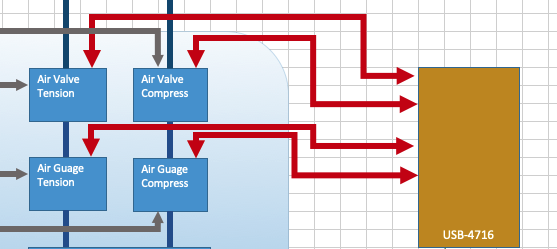
\includegraphics[width=3.12500in]{jira_imgs/3435.png}

}
\hdashrule[0.5ex]{\textwidth}{1pt}{3mm}
  Expected Result \\
{\footnotesize
The air valves and gauges are hooked up to the USB-4716 readout device.~

}
\hdashrule[0.5ex]{\textwidth}{1pt}{3mm}
  Actual Result \\
{\footnotesize

}
\begin{tabular}{p{2cm}p{14cm}}
\toprule
Step 6 & Step Execution Status: \textbf{ Not Executed } \\ \hline
\end{tabular}
 Description \\
{\footnotesize
Make the connection between the MB5U readout electronics and the
renishaw encoders.

}
\hdashrule[0.5ex]{\textwidth}{1pt}{3mm}
  Expected Result \\
{\footnotesize
The MB5U readouts are connected to the encoders.

}
\hdashrule[0.5ex]{\textwidth}{1pt}{3mm}
  Actual Result \\
{\footnotesize

}
\begin{tabular}{p{2cm}p{14cm}}
\toprule
Step 7 & Step Execution Status: \textbf{ Not Executed } \\ \hline
\end{tabular}
 Description \\
{\footnotesize
Make the connection between the 9150 load cell readout electronic and
the load cell.

}
\hdashrule[0.5ex]{\textwidth}{1pt}{3mm}
  Expected Result \\
{\footnotesize
The load cell is connected to the load cell readout electronic.

}
\hdashrule[0.5ex]{\textwidth}{1pt}{3mm}
  Actual Result \\
{\footnotesize

}
\begin{tabular}{p{2cm}p{14cm}}
\toprule
Step 8 & Step Execution Status: \textbf{ Not Executed } \\ \hline
\end{tabular}
 Description \\
{\footnotesize
Make the connection between the Hexapod Actuator to the thermal
scanner.~

}
\hdashrule[0.5ex]{\textwidth}{1pt}{3mm}
  Expected Result \\
{\footnotesize
The thermal scanner is connected to the hexapod actuator.

}
\hdashrule[0.5ex]{\textwidth}{1pt}{3mm}
  Actual Result \\
{\footnotesize

}
\begin{tabular}{p{2cm}p{14cm}}
\toprule
Step 9 & Step Execution Status: \textbf{ Not Executed } \\ \hline
\end{tabular}
 Description \\
{\footnotesize
Connect the following to the USB 3.0 Hub:

\begin{itemize}
\tightlist
\item
  (2) connections for MB5U Readout Electronic
\item
  USB-4716 Readout Device/Labjack T4
\item
  Temperature Readout
\item
  9150 Load Cell Readout Electronic
\end{itemize}

}
\hdashrule[0.5ex]{\textwidth}{1pt}{3mm}
  Expected Result \\
{\footnotesize
The USB 3.0 Hub is now connected to the readout electronics from the
previous steps.~

}
\hdashrule[0.5ex]{\textwidth}{1pt}{3mm}
  Actual Result \\
{\footnotesize

}
\begin{tabular}{p{2cm}p{14cm}}
\toprule
Step 10 & Step Execution Status: \textbf{ Not Executed } \\ \hline
\end{tabular}
 Description \\
{\footnotesize
Connect the laptop with LabVIEW software to the USB 3.0 Hub.

}
\hdashrule[0.5ex]{\textwidth}{1pt}{3mm}
  Expected Result \\
{\footnotesize
The Laptop is connected to the USB 3.0 Hub and to the subsequent readout
electronics.~

}
\hdashrule[0.5ex]{\textwidth}{1pt}{3mm}
  Actual Result \\
{\footnotesize

}
\begin{tabular}{p{2cm}p{14cm}}
\toprule
Step 11 & Step Execution Status: \textbf{ Not Executed } \\ \hline
\end{tabular}
 Description \\
{\footnotesize
Connect the laptop to the Copley Motor drive of the Control Box.

}
\hdashrule[0.5ex]{\textwidth}{1pt}{3mm}
  Expected Result \\
{\footnotesize
The laptop is connected to the control box.

}
\hdashrule[0.5ex]{\textwidth}{1pt}{3mm}
  Actual Result \\
{\footnotesize

}
\begin{tabular}{p{2cm}p{14cm}}
\toprule
Step 12 & Step Execution Status: \textbf{ Not Executed } \\ \hline
\end{tabular}
 Description \\
{\footnotesize
Set up the USB 3.0 Hub close to the test fixture and connect it to a
power source.~

}
\hdashrule[0.5ex]{\textwidth}{1pt}{3mm}
  Expected Result \\
{\footnotesize
The USB 3.0 Hub is connected and all readout devices are powered on.~

}
\hdashrule[0.5ex]{\textwidth}{1pt}{3mm}
  Actual Result \\
{\footnotesize

}
\begin{tabular}{p{2cm}p{14cm}}
\toprule
Step 13 & Step Execution Status: \textbf{ Not Executed } \\ \hline
\end{tabular}
 Description \\
{\footnotesize
Verify that the output data from the readout devices are available on
the laptop.

}
\hdashrule[0.5ex]{\textwidth}{1pt}{3mm}
  Expected Result \\
{\footnotesize
The laptop is seen to be able to communicate with the readout devices.

}
\hdashrule[0.5ex]{\textwidth}{1pt}{3mm}
  Actual Result \\
{\footnotesize

}
\begin{tabular}{p{2cm}p{14cm}}
\toprule
Step 14 & Step Execution Status: \textbf{ Not Executed } \\ \hline
\end{tabular}
 Description \\
{\footnotesize
Open Labview 2021 in the computer used for Test Setup.

}
\hdashrule[0.5ex]{\textwidth}{1pt}{3mm}
  Expected Result \\
{\footnotesize
Labview 2021 opens successfully.

}
\hdashrule[0.5ex]{\textwidth}{1pt}{3mm}
  Actual Result \\
{\footnotesize

}
\begin{tabular}{p{2cm}p{14cm}}
\toprule
Step 15 & Step Execution Status: \textbf{ Not Executed } \\ \hline
\end{tabular}
 Description \\
{\footnotesize
Open the Labview VI files from the project directory including sub VIs-
Tovey Closed loop.vi, Voltage Regulation.vi and Biss Reader.vi

}
\hdashrule[0.5ex]{\textwidth}{1pt}{3mm}
  Expected Result \\
{\footnotesize
Front panel of VI and sub VI files open without any error.

}
\hdashrule[0.5ex]{\textwidth}{1pt}{3mm}
  Actual Result \\
{\footnotesize

}
\begin{tabular}{p{2cm}p{14cm}}
\toprule
Step 16 & Step Execution Status: \textbf{ Not Executed } \\ \hline
\end{tabular}
 Description \\
{\footnotesize
Configure the Biss Reader.vi file with the appropriate configuration
file and following the IBISS operation manual.~

}
\hdashrule[0.5ex]{\textwidth}{1pt}{3mm}
  Expected Result \\
{\footnotesize
\href{https://jira.lsstcorp.org/rest/tests/1.0/attachment/3555}{BiSS\_config.cfg}
is loaded in the LabView configuration (Misc Tab under Load DLL). The
configuration file is based on the IBISS operation manual.

}
\hdashrule[0.5ex]{\textwidth}{1pt}{3mm}
  Actual Result \\
{\footnotesize

}
\begin{tabular}{p{2cm}p{14cm}}
\toprule
Step 17 & Step Execution Status: \textbf{ Not Executed } \\ \hline
\end{tabular}
 Description \\
{\footnotesize
Click Run button on the on the block diagram toolbar of the Labview VI
front panel.

}
\hdashrule[0.5ex]{\textwidth}{1pt}{3mm}
  Expected Result \\
{\footnotesize
LabView VI and ~associated sub Vi runs successfully. Initially all the
graphs and input values will be blank.

}
\hdashrule[0.5ex]{\textwidth}{1pt}{3mm}
  Actual Result \\
{\footnotesize

}
\begin{tabular}{p{2cm}p{14cm}}
\toprule
Step 18 & Step Execution Status: \textbf{ Not Executed } \\ \hline
\end{tabular}
 Description \\
{\footnotesize
Send a command through LabVIEW ~voltage Regulation.vi to set the voltage
on the compression valve only to 3V.

}
\hdashrule[0.5ex]{\textwidth}{1pt}{3mm}
  Expected Result \\
{\footnotesize
The command is accepted, the pneumatic valve shows the applied voltage
only on the compression valve and the applied compression force can be
seen on the LabView front panel Time vs Load graph.~

}
\hdashrule[0.5ex]{\textwidth}{1pt}{3mm}
  Actual Result \\
{\footnotesize

}
\begin{tabular}{p{2cm}p{14cm}}
\toprule
Step 19 & Step Execution Status: \textbf{ Not Executed } \\ \hline
\end{tabular}
 Description \\
{\footnotesize
Send a command through LabVIEW voltage Regulation.vi to reset the
compression valve to 0V.

}
\hdashrule[0.5ex]{\textwidth}{1pt}{3mm}
  Expected Result \\
{\footnotesize
The command is accepted. The applied force can be seen as zero load on
the LabView front panel Time vs Load graph. Load Cell Reader also shows
zero load.

}
\hdashrule[0.5ex]{\textwidth}{1pt}{3mm}
  Actual Result \\
{\footnotesize

}
\begin{tabular}{p{2cm}p{14cm}}
\toprule
Step 20 & Step Execution Status: \textbf{ Not Executed } \\ \hline
\end{tabular}
 Description \\
{\footnotesize
Send a command through LabVIEW to reset the tension valve to 3V.

}
\hdashrule[0.5ex]{\textwidth}{1pt}{3mm}
  Expected Result \\
{\footnotesize
The command is accepted, the readout electronic shows the applied
voltage only on the tension valve and the applied tension force can be
seen on the LabView front panel Time vs Load graph.

}
\hdashrule[0.5ex]{\textwidth}{1pt}{3mm}
  Actual Result \\
{\footnotesize

}
\begin{tabular}{p{2cm}p{14cm}}
\toprule
Step 21 & Step Execution Status: \textbf{ Not Executed } \\ \hline
\end{tabular}
 Description \\
{\footnotesize
Send a command through LabVIEW to reset the tension valve to 0V.

}
\hdashrule[0.5ex]{\textwidth}{1pt}{3mm}
  Expected Result \\
{\footnotesize
The command is accepted, the readout electronic no longer shows the
applied voltage on the tension valve and there is no longer any tension
force on the LabView front panel Time vs Load graph.

}
\hdashrule[0.5ex]{\textwidth}{1pt}{3mm}
  Actual Result \\
{\footnotesize

}
\begin{tabular}{p{2cm}p{14cm}}
\toprule
Step 22 & Step Execution Status: \textbf{ Not Executed } \\ \hline
\end{tabular}
 Description \\
{\footnotesize
Verify the laptop is reading the renishaw scales usinthe Biss Reader.vi
file and determine the zero stroke position.

}
\hdashrule[0.5ex]{\textwidth}{1pt}{3mm}
  Test Data \\
 {\footnotesize
\textbf{Note:~}Moog's original test procedure cited the zero position to
be at 40mm since the full length was 80mm.

}
\hdashrule[0.5ex]{\textwidth}{1pt}{3mm}
  Expected Result \\
{\footnotesize
40mm encoder readings shown in Labview front panel of the .vi file.~\\
The zero stroke position has been determined and can be used as a
reference for the offset of future moves.

}
\hdashrule[0.5ex]{\textwidth}{1pt}{3mm}
  Actual Result \\
{\footnotesize

}
\begin{tabular}{p{2cm}p{14cm}}
\toprule
Step 23 & Step Execution Status: \textbf{ Not Executed } \\ \hline
\end{tabular}
 Description \\
{\footnotesize
Using the Copley Software, drive the actuator to the positive limit
switch and take note of the values measured by the Copley Software and
the Encoder Readings.

}
\hdashrule[0.5ex]{\textwidth}{1pt}{3mm}
  Expected Result \\
{\footnotesize
The actuator is able to hit the positive limit switch and the values are
recorded.

}
\hdashrule[0.5ex]{\textwidth}{1pt}{3mm}
  Actual Result \\
{\footnotesize

}
\begin{tabular}{p{2cm}p{14cm}}
\toprule
Step 24 & Step Execution Status: \textbf{ Not Executed } \\ \hline
\end{tabular}
 Description \\
{\footnotesize
Using the Copley Software, drive the actuator to the negative limit
switch and take note of the values measured by the Copley Software and
the Encoder Readings.

}
\hdashrule[0.5ex]{\textwidth}{1pt}{3mm}
  Expected Result \\
{\footnotesize
The actuator is able to hit the negative limit switch and the values are
recorded.

}
\hdashrule[0.5ex]{\textwidth}{1pt}{3mm}
  Actual Result \\
{\footnotesize

}

\paragraph{ LVV-T2426 - Hexapod - Actuator Proofing Testing with 200\% load }\mbox{}\\

Version \textbf{1}.
Status \textbf{Approved}.
Open  \href{https://jira.lsstcorp.org/secure/Tests.jspa#/testCase/LVV-T2426}{\textit{ LVV-T2426 } }
test case in Jira.

To perform the actuator proofing test with 200\% load in order to verify
the \citeds{LTS-206} hexapod proof testing requirement.~

\textbf{ Preconditions}:\\


Execution status: {\bf Not Executed }

Final comment:\\


Detailed steps results:

\begin{tabular}{p{2cm}p{14cm}}
\toprule
Step 1 & Step Execution Status: \textbf{ Not Executed } \\ \hline
\end{tabular}
 Description \\
{\footnotesize
Open Labview 2021 in the computer used for Test Setup.

}
\hdashrule[0.5ex]{\textwidth}{1pt}{3mm}
  Test Data \\
 {\footnotesize
\textbf{Note:~}The first three steps are conditional because these steps
are included as part of the Test Setup procedure and may not be
necessary if LabView is still open.

}
\hdashrule[0.5ex]{\textwidth}{1pt}{3mm}
  Expected Result \\
{\footnotesize
Labview 2021 opens successfully.

}
\hdashrule[0.5ex]{\textwidth}{1pt}{3mm}
  Actual Result \\
{\footnotesize

}
\begin{tabular}{p{2cm}p{14cm}}
\toprule
Step 2 & Step Execution Status: \textbf{ Not Executed } \\ \hline
\end{tabular}
 Description \\
{\footnotesize
Run the following VI's:

\begin{itemize}
\tightlist
\item
  Encoder A (D13B) and Load Cell.vi
\item
  Encoder B (D0BD).vi
\end{itemize}

}
\hdashrule[0.5ex]{\textwidth}{1pt}{3mm}
  Expected Result \\
{\footnotesize
Front panel of VI's open without any error.

}
\hdashrule[0.5ex]{\textwidth}{1pt}{3mm}
  Actual Result \\
{\footnotesize

}
\begin{tabular}{p{2cm}p{14cm}}
\toprule
Step 3 & Step Execution Status: \textbf{ Not Executed } \\ \hline
\end{tabular}
 Description \\
{\footnotesize
Click Run button on the on the block diagram toolbar of the Labview VI
front panel.

}
\hdashrule[0.5ex]{\textwidth}{1pt}{3mm}
  Expected Result \\
{\footnotesize
LabView VI and associated sub Vi runs successfully. The graphs should
start to be populated with data once the run button is pressed.

}
\hdashrule[0.5ex]{\textwidth}{1pt}{3mm}
  Actual Result \\
{\footnotesize

}
\begin{tabular}{p{2cm}p{14cm}}
\toprule
Step 4 & Step Execution Status: \textbf{ Not Executed } \\ \hline
\end{tabular}
 Description \\
{\footnotesize
Position the actuator at its center of stroke position using the control
box and copley software.~

}
\hdashrule[0.5ex]{\textwidth}{1pt}{3mm}
  Expected Result \\
{\footnotesize
Actuator positioned at its center of stroke position ~confirmed by
encoder reading in the LabView.

}
\hdashrule[0.5ex]{\textwidth}{1pt}{3mm}
  Actual Result \\
{\footnotesize

}
\begin{tabular}{p{2cm}p{14cm}}
\toprule
Step 5 & Step Execution Status: \textbf{ Not Executed } \\ \hline
\end{tabular}
 Description \\
{\footnotesize
Disable Motor Power by pressing the Emergency stop button on the control
box.

}
\hdashrule[0.5ex]{\textwidth}{1pt}{3mm}
  Expected Result \\
{\footnotesize
Motor power disabled.~

}
\hdashrule[0.5ex]{\textwidth}{1pt}{3mm}
  Actual Result \\
{\footnotesize

}
\begin{tabular}{p{2cm}p{14cm}}
\toprule
Step 6 & Step Execution Status: \textbf{ Not Executed } \\ \hline
\end{tabular}
 Description \\
{\footnotesize
Slowly apply an increasing tension force with the load actuator until a
force of 60 kN (13,489 lbf) through the Encoder A (D13B) and Load
Cell.vi

}
\hdashrule[0.5ex]{\textwidth}{1pt}{3mm}
  Test Data \\
 {\footnotesize
\textbf{Note:~}Set valve to 8.76V to apply a +/-60kN force.

}
\hdashrule[0.5ex]{\textwidth}{1pt}{3mm}
  Expected Result \\
{\footnotesize
Tension force applied to the actuator increasingly.

}
\hdashrule[0.5ex]{\textwidth}{1pt}{3mm}
  Actual Result \\
{\footnotesize

}
\begin{tabular}{p{2cm}p{14cm}}
\toprule
Step 7 & Step Execution Status: \textbf{ Not Executed } \\ \hline
\end{tabular}
 Description \\
{\footnotesize
Make sure the load does not go over 60 kN, as this load represents the
2X the max load or proof test load case.~

}
\hdashrule[0.5ex]{\textwidth}{1pt}{3mm}
  Expected Result \\
{\footnotesize
In the LabView load graph and load cell reader, showing the 60 KN
tension force.

}
\hdashrule[0.5ex]{\textwidth}{1pt}{3mm}
  Actual Result \\
{\footnotesize

}
\begin{tabular}{p{2cm}p{14cm}}
\toprule
Step 8 & Step Execution Status: \textbf{ Not Executed } \\ \hline
\end{tabular}
 Description \\
{\footnotesize
Continue to apply the load for 10 minutes and observe for any unexpected
movement or sounds. Check for the Encoder Readings in the Time vs
Displacement graphs on the Labview BISS Reader VI for 10 minutes.~

}
\hdashrule[0.5ex]{\textwidth}{1pt}{3mm}
  Test Data \\
 {\footnotesize
\textbf{Note:~}Maintain the force on the cell by keeping the same
voltage in the LabView voltage regulation VI.

}
\hdashrule[0.5ex]{\textwidth}{1pt}{3mm}
  Expected Result \\
{\footnotesize
No unexpected movement or sounds recorded to indicate any catastrophic
failure.

}
\hdashrule[0.5ex]{\textwidth}{1pt}{3mm}
  Actual Result \\
{\footnotesize

}
\begin{tabular}{p{2cm}p{14cm}}
\toprule
Step 9 & Step Execution Status: \textbf{ Not Executed } \\ \hline
\end{tabular}
 Description \\
{\footnotesize
Slowly remove the tension force to return to zero load.~

}
\hdashrule[0.5ex]{\textwidth}{1pt}{3mm}
  Expected Result \\
{\footnotesize
Tension force removed and load cell reading in the lab-view graph and
load cell reader showing zero load.

}
\hdashrule[0.5ex]{\textwidth}{1pt}{3mm}
  Actual Result \\
{\footnotesize

}
\begin{tabular}{p{2cm}p{14cm}}
\toprule
Step 10 & Step Execution Status: \textbf{ Not Executed } \\ \hline
\end{tabular}
 Description \\
{\footnotesize
Return the position the actuator to its center of stroke position using
the control box and copley software..

}
\hdashrule[0.5ex]{\textwidth}{1pt}{3mm}
  Test Data \\
 {\footnotesize
\textbf{Note:~}This is where the linear encoder reads 40mm.~

}
\hdashrule[0.5ex]{\textwidth}{1pt}{3mm}
  Expected Result \\
{\footnotesize
Actuator positioned at its center of stroke position ~confirmed by
encoder reading in the LabView.

}
\hdashrule[0.5ex]{\textwidth}{1pt}{3mm}
  Actual Result \\
{\footnotesize

}
\begin{tabular}{p{2cm}p{14cm}}
\toprule
Step 11 & Step Execution Status: \textbf{ Not Executed } \\ \hline
\end{tabular}
 Description \\
{\footnotesize
Slowly apply an increasing compression force with the load actuator
until a force of 60 kN (13,489 lbf) is reached using Lab view Vi
regulator.~

}
\hdashrule[0.5ex]{\textwidth}{1pt}{3mm}
  Test Data \\
 {\footnotesize
\textbf{Note:~}Set valve to 8.76V to apply a +/-60kN force.

}
\hdashrule[0.5ex]{\textwidth}{1pt}{3mm}
  Expected Result \\
{\footnotesize
Load graph and Load Cell Reader showing 60 kN compression force applied
to the actuator increasingly.

}
\hdashrule[0.5ex]{\textwidth}{1pt}{3mm}
  Actual Result \\
{\footnotesize

}
\begin{tabular}{p{2cm}p{14cm}}
\toprule
Step 12 & Step Execution Status: \textbf{ Not Executed } \\ \hline
\end{tabular}
 Description \\
{\footnotesize
Make sure the load does not go over 60 kN ~as this load represents the
2X the max load or proof test load case.

}
\hdashrule[0.5ex]{\textwidth}{1pt}{3mm}
  Expected Result \\
{\footnotesize
In the LabView load graph,load does not surpass 60 kN.

}
\hdashrule[0.5ex]{\textwidth}{1pt}{3mm}
  Actual Result \\
{\footnotesize

}
\begin{tabular}{p{2cm}p{14cm}}
\toprule
Step 13 & Step Execution Status: \textbf{ Not Executed } \\ \hline
\end{tabular}
 Description \\
{\footnotesize
Continue to apply the load for 10 minutes and observe for any unexpected
movement or sounds.

}
\hdashrule[0.5ex]{\textwidth}{1pt}{3mm}
  Expected Result \\
{\footnotesize
\textbf{No unexpected movement or sounds recorded to indicate any
catastrophic failure.}

}
\hdashrule[0.5ex]{\textwidth}{1pt}{3mm}
  Actual Result \\
{\footnotesize

}
\begin{tabular}{p{2cm}p{14cm}}
\toprule
Step 14 & Step Execution Status: \textbf{ Not Executed } \\ \hline
\end{tabular}
 Description \\
{\footnotesize
Slowly remove the compression force to return to the zero load.

}
\hdashrule[0.5ex]{\textwidth}{1pt}{3mm}
  Expected Result \\
{\footnotesize
Compression force removed and load cell reading in the lab-view graph
and load cell reader showing zero load.

}
\hdashrule[0.5ex]{\textwidth}{1pt}{3mm}
  Actual Result \\
{\footnotesize

}
\begin{tabular}{p{2cm}p{14cm}}
\toprule
Step 15 & Step Execution Status: \textbf{ Not Executed } \\ \hline
\end{tabular}
 Description \\
{\footnotesize
Press Stop button in the VI file front panel to stop reading of the
components

}
\hdashrule[0.5ex]{\textwidth}{1pt}{3mm}
  Expected Result \\
{\footnotesize
Graphs in the front panel of the VI file becomes static.

}
\hdashrule[0.5ex]{\textwidth}{1pt}{3mm}
  Actual Result \\
{\footnotesize

}
\begin{tabular}{p{2cm}p{14cm}}
\toprule
Step 16 & Step Execution Status: \textbf{ Not Executed } \\ \hline
\end{tabular}
 Description \\
{\footnotesize
Check if all the test results are recorded in excel spreadsheets.

}
\hdashrule[0.5ex]{\textwidth}{1pt}{3mm}
  Expected Result \\
{\footnotesize
Test Results are recorded in the excel spreadsheets residing in the
LabView Folder directory.

}
\hdashrule[0.5ex]{\textwidth}{1pt}{3mm}
  Actual Result \\
{\footnotesize

}
\begin{tabular}{p{2cm}p{14cm}}
\toprule
Step 17 & Step Execution Status: \textbf{ Not Executed } \\ \hline
\end{tabular}
 Description \\
{\footnotesize
Close all the Labview VI files.

}
\hdashrule[0.5ex]{\textwidth}{1pt}{3mm}
  Test Data \\
 {\footnotesize
\textbf{Note:} Labview can be left open in order to continue to the next
test. However, it may be necessary to reset the application before
starting the next test.

}
\hdashrule[0.5ex]{\textwidth}{1pt}{3mm}
  Expected Result \\
{\footnotesize
All the VI files are closed and Labview 2021 application window closes.

}
\hdashrule[0.5ex]{\textwidth}{1pt}{3mm}
  Actual Result \\
{\footnotesize

}

\paragraph{ LVV-T2427 - Hexapod - Actuator Back Driving Test }\mbox{}\\

Version \textbf{1}.
Status \textbf{Approved}.
Open  \href{https://jira.lsstcorp.org/secure/Tests.jspa#/testCase/LVV-T2427}{\textit{ LVV-T2427 } }
test case in Jira.

The objective of this test case is to verify that removing the power
from an actuator will not cause the actuator to back drive even with the
application of different loads.

\textbf{ Preconditions}:\\
Proofing 200\% load test should be performed before running the
back-driving test.~

Execution status: {\bf Not Executed }

Final comment:\\


Detailed steps results:

\begin{tabular}{p{2cm}p{14cm}}
\toprule
Step 1 & Step Execution Status: \textbf{ Not Executed } \\ \hline
\end{tabular}
 Description \\
{\footnotesize
Open Labview 2021 in the computer used for Test Setup.

}
\hdashrule[0.5ex]{\textwidth}{1pt}{3mm}
  Test Data \\
 {\footnotesize
\textbf{Note:~}The first three steps are conditional because these steps
are included as part of the Test Setup procedure and may not be
necessary if LabView is still open.

}
\hdashrule[0.5ex]{\textwidth}{1pt}{3mm}
  Expected Result \\
{\footnotesize
Labview 2021 opens successfully.

}
\hdashrule[0.5ex]{\textwidth}{1pt}{3mm}
  Actual Result \\
{\footnotesize

}
\begin{tabular}{p{2cm}p{14cm}}
\toprule
Step 2 & Step Execution Status: \textbf{ Not Executed } \\ \hline
\end{tabular}
 Description \\
{\footnotesize
Open Labview 2021 in the computer used for Test Setup.

}
\hdashrule[0.5ex]{\textwidth}{1pt}{3mm}
  Test Data \\
 {\footnotesize
\textbf{Note:~}The first three steps are conditional because these steps
are included as part of the Test Setup procedure and may not be
necessary if LabView is still open.

}
\hdashrule[0.5ex]{\textwidth}{1pt}{3mm}
  Expected Result \\
{\footnotesize
Labview 2021 opens successfully.

}
\hdashrule[0.5ex]{\textwidth}{1pt}{3mm}
  Actual Result \\
{\footnotesize

}
\begin{tabular}{p{2cm}p{14cm}}
\toprule
Step 3 & Step Execution Status: \textbf{ Not Executed } \\ \hline
\end{tabular}
 Description \\
{\footnotesize
Run the following VI's:

\begin{itemize}
\tightlist
\item
  Encoder A (D13B) and Load Cell.vi
\item
  Encoder B (D0BD).vi
\end{itemize}

}
\hdashrule[0.5ex]{\textwidth}{1pt}{3mm}
  Test Data \\
 {\footnotesize
\textbf{Note:~}Each vi is responsible for reading one encoder.

}
\hdashrule[0.5ex]{\textwidth}{1pt}{3mm}
  Expected Result \\
{\footnotesize
Front panel of VI's open without any error.

}
\hdashrule[0.5ex]{\textwidth}{1pt}{3mm}
  Actual Result \\
{\footnotesize

}
\begin{tabular}{p{2cm}p{14cm}}
\toprule
Step 4 & Step Execution Status: \textbf{ Not Executed } \\ \hline
\end{tabular}
 Description \\
{\footnotesize
Run the following VI's:

\begin{itemize}
\tightlist
\item
  Encoder A (D13B) and Load Cell.vi
\item
  Encoder B (D0BD).vi
\end{itemize}

}
\hdashrule[0.5ex]{\textwidth}{1pt}{3mm}
  Test Data \\
 {\footnotesize
\textbf{Note:~}Each vi is responsible for reading one encoder.

}
\hdashrule[0.5ex]{\textwidth}{1pt}{3mm}
  Expected Result \\
{\footnotesize
Front panel of VI's open without any error.

}
\hdashrule[0.5ex]{\textwidth}{1pt}{3mm}
  Actual Result \\
{\footnotesize

}
\begin{tabular}{p{2cm}p{14cm}}
\toprule
Step 5 & Step Execution Status: \textbf{ Not Executed } \\ \hline
\end{tabular}
 Description \\
{\footnotesize
Click Run button on the block diagram toolbar of the Labview VI front
panel.

}
\hdashrule[0.5ex]{\textwidth}{1pt}{3mm}
  Expected Result \\
{\footnotesize
LabView VI and associated sub Vi runs successfully. The graphs should
start to be populated with data once the run button is pressed.

}
\hdashrule[0.5ex]{\textwidth}{1pt}{3mm}
  Actual Result \\
{\footnotesize

}
\begin{tabular}{p{2cm}p{14cm}}
\toprule
Step 6 & Step Execution Status: \textbf{ Not Executed } \\ \hline
\end{tabular}
 Description \\
{\footnotesize
Click Run button on the block diagram toolbar of the Labview VI front
panel.

}
\hdashrule[0.5ex]{\textwidth}{1pt}{3mm}
  Expected Result \\
{\footnotesize
LabView VI and associated sub Vi runs successfully. The graphs should
start to be populated with data once the run button is pressed.

}
\hdashrule[0.5ex]{\textwidth}{1pt}{3mm}
  Actual Result \\
{\footnotesize

}
\begin{tabular}{p{2cm}p{14cm}}
\toprule
Step 7 & Step Execution Status: \textbf{ Not Executed } \\ \hline
\end{tabular}
 Description \\
{\footnotesize
Record the starting position of the actuator using the external
encoders.

}
\hdashrule[0.5ex]{\textwidth}{1pt}{3mm}
  Test Data \\
 {\footnotesize
\textbf{Note:~}The Copley software will display a value based on the
reading from its internal encoder, which may be useful to take note of.
However, the readings reported by the external encoders will validate
the reading of the internal encoder.

}
\hdashrule[0.5ex]{\textwidth}{1pt}{3mm}
  Expected Result \\
{\footnotesize
The actuator position is determined by the external encoders.

}
\hdashrule[0.5ex]{\textwidth}{1pt}{3mm}
  Actual Result \\
{\footnotesize

}
\begin{tabular}{p{2cm}p{14cm}}
\toprule
Step 8 & Step Execution Status: \textbf{ Not Executed } \\ \hline
\end{tabular}
 Description \\
{\footnotesize
Record the starting position of the actuator using the external
encoders.

}
\hdashrule[0.5ex]{\textwidth}{1pt}{3mm}
  Test Data \\
 {\footnotesize
\textbf{Note:~}The Copley software will display a value based on the
reading from its internal encoder, which may be useful to take note of.
However, the readings reported by the external encoders will validate
the reading of the internal encoder.

}
\hdashrule[0.5ex]{\textwidth}{1pt}{3mm}
  Expected Result \\
{\footnotesize
The actuator position is determined by the external encoders.

}
\hdashrule[0.5ex]{\textwidth}{1pt}{3mm}
  Actual Result \\
{\footnotesize

}
\begin{tabular}{p{2cm}p{14cm}}
\toprule
Step 9 & Step Execution Status: \textbf{ Not Executed } \\ \hline
\end{tabular}
 Description \\
{\footnotesize
Make sure motor drive is disabled using Copley software and the control
box.~

}
\hdashrule[0.5ex]{\textwidth}{1pt}{3mm}
  Expected Result \\
{\footnotesize
Motor drive is disabled.~

}
\hdashrule[0.5ex]{\textwidth}{1pt}{3mm}
  Actual Result \\
{\footnotesize

}
\begin{tabular}{p{2cm}p{14cm}}
\toprule
Step 10 & Step Execution Status: \textbf{ Not Executed } \\ \hline
\end{tabular}
 Description \\
{\footnotesize
Make sure motor drive is disabled using Copley software and the control
box.~

}
\hdashrule[0.5ex]{\textwidth}{1pt}{3mm}
  Expected Result \\
{\footnotesize
Motor drive is disabled.~

}
\hdashrule[0.5ex]{\textwidth}{1pt}{3mm}
  Actual Result \\
{\footnotesize

}
\begin{tabular}{p{2cm}p{14cm}}
\toprule
Step 11 & Step Execution Status: \textbf{ Not Executed } \\ \hline
\end{tabular}
 Description \\
{\footnotesize
Slowly apply an increasing {Tension}⁠ ~force of +/-37.5kN.~

}
\hdashrule[0.5ex]{\textwidth}{1pt}{3mm}
  Test Data \\
 {\footnotesize
\textbf{Note:~}Set the {Tension}⁠ valve to 5.48V in order to apply
+/-37.5kN of force.

}
\hdashrule[0.5ex]{\textwidth}{1pt}{3mm}
  Expected Result \\
{\footnotesize
Load cell reader shows the applied +/-37.5kN {Tension}⁠~ force.\\
LabView displays the voltage being applied.

}
\hdashrule[0.5ex]{\textwidth}{1pt}{3mm}
  Actual Result \\
{\footnotesize

}
\begin{tabular}{p{2cm}p{14cm}}
\toprule
Step 12 & Step Execution Status: \textbf{ Not Executed } \\ \hline
\end{tabular}
 Description \\
{\footnotesize
Slowly apply an increasing {Compression}⁠ ~force of +/-37.5kN.~

}
\hdashrule[0.5ex]{\textwidth}{1pt}{3mm}
  Test Data \\
 {\footnotesize
\textbf{Note:~}Set the {Compression}⁠ valve to 5.48V in order to apply
+/-37.5kN of force.

}
\hdashrule[0.5ex]{\textwidth}{1pt}{3mm}
  Expected Result \\
{\footnotesize
Load cell reader shows the applied +/-37.5kN {Compression}⁠~ force.\\
LabView displays the voltage being applied.

}
\hdashrule[0.5ex]{\textwidth}{1pt}{3mm}
  Actual Result \\
{\footnotesize

}
\begin{tabular}{p{2cm}p{14cm}}
\toprule
Step 13 & Step Execution Status: \textbf{ Not Executed } \\ \hline
\end{tabular}
 Description \\
{\footnotesize
Record the displacement of the actuator using the external encoder
readings.

}
\hdashrule[0.5ex]{\textwidth}{1pt}{3mm}
  Test Data \\
 {\footnotesize
\textbf{Note:~}The Copley software will display a value based on the
reading from its internal encoder, which may be useful to take note of.
However, the readings reported by the external encoders will validate
the reading of the internal encoder.

}
\hdashrule[0.5ex]{\textwidth}{1pt}{3mm}
  Expected Result \\
{\footnotesize
The final position of the actuator has been determined.\\
If the actuator position has changed significantly (\textgreater{}10
counts or 0.36 deg of motor rotation), the actuator has back-driven.

}
\hdashrule[0.5ex]{\textwidth}{1pt}{3mm}
  Actual Result \\
{\footnotesize

}
\begin{tabular}{p{2cm}p{14cm}}
\toprule
Step 14 & Step Execution Status: \textbf{ Not Executed } \\ \hline
\end{tabular}
 Description \\
{\footnotesize
Record the displacement of the actuator using the external encoder
readings.

}
\hdashrule[0.5ex]{\textwidth}{1pt}{3mm}
  Test Data \\
 {\footnotesize
\textbf{Note:~}The Copley software will display a value based on the
reading from its internal encoder, which may be useful to take note of.
However, the readings reported by the external encoders will validate
the reading of the internal encoder.

}
\hdashrule[0.5ex]{\textwidth}{1pt}{3mm}
  Expected Result \\
{\footnotesize
The final position of the actuator has been determined.\\
If the actuator position has changed significantly (\textgreater{}10
counts or 0.36 deg of motor rotation), the actuator has back-driven.

}
\hdashrule[0.5ex]{\textwidth}{1pt}{3mm}
  Actual Result \\
{\footnotesize

}
\begin{tabular}{p{2cm}p{14cm}}
\toprule
Step 15 & Step Execution Status: \textbf{ Not Executed } \\ \hline
\end{tabular}
 Description \\
{\footnotesize
Confirm that there are no other signs of gross actuator motion.

}
\hdashrule[0.5ex]{\textwidth}{1pt}{3mm}
  Expected Result \\
{\footnotesize
No visual movement, significant motion of the internal linear encoder or
external linear test encoders beyond expected actuator compliance
recorded in the LabView displacement graphs.~

}
\hdashrule[0.5ex]{\textwidth}{1pt}{3mm}
  Actual Result \\
{\footnotesize

}
\begin{tabular}{p{2cm}p{14cm}}
\toprule
Step 16 & Step Execution Status: \textbf{ Not Executed } \\ \hline
\end{tabular}
 Description \\
{\footnotesize
Confirm that there are no other signs of gross actuator motion.

}
\hdashrule[0.5ex]{\textwidth}{1pt}{3mm}
  Expected Result \\
{\footnotesize
No visual movement, significant motion of the internal linear encoder or
external linear test encoders beyond expected actuator compliance
recorded in the LabView displacement graphs.~

}
\hdashrule[0.5ex]{\textwidth}{1pt}{3mm}
  Actual Result \\
{\footnotesize

}
\begin{tabular}{p{2cm}p{14cm}}
\toprule
Step 17 & Step Execution Status: \textbf{ Not Executed } \\ \hline
\end{tabular}
 Description \\
{\footnotesize
Reduce the {Tension}⁠ ~force to back to zero load.

}
\hdashrule[0.5ex]{\textwidth}{1pt}{3mm}
  Test Data \\
 {\footnotesize
\textbf{Note:~}In order to reset the load to zero, both the valves
should be set to 0V.

}
\hdashrule[0.5ex]{\textwidth}{1pt}{3mm}
  Expected Result \\
{\footnotesize
{Tension}⁠~ force removed and load cell reading in the lab-view graph
and load cell reader showing zero load.

}
\hdashrule[0.5ex]{\textwidth}{1pt}{3mm}
  Actual Result \\
{\footnotesize

}
\begin{tabular}{p{2cm}p{14cm}}
\toprule
Step 18 & Step Execution Status: \textbf{ Not Executed } \\ \hline
\end{tabular}
 Description \\
{\footnotesize
Reduce the {Compression}⁠ ~force to back to zero load.

}
\hdashrule[0.5ex]{\textwidth}{1pt}{3mm}
  Test Data \\
 {\footnotesize
\textbf{Note:~}In order to reset the load to zero, both the valves
should be set to 0V.

}
\hdashrule[0.5ex]{\textwidth}{1pt}{3mm}
  Expected Result \\
{\footnotesize
{Compression}⁠~ force removed and load cell reading in the lab-view
graph and load cell reader showing zero load.

}
\hdashrule[0.5ex]{\textwidth}{1pt}{3mm}
  Actual Result \\
{\footnotesize

}
\begin{tabular}{p{2cm}p{14cm}}
\toprule
Step 19 & Step Execution Status: \textbf{ Not Executed } \\ \hline
\end{tabular}
 Description \\
{\footnotesize
Record the displacement of the actuator using the external encoder
readings.

}
\hdashrule[0.5ex]{\textwidth}{1pt}{3mm}
  Test Data \\
 {\footnotesize
\textbf{Note:~}The Copley software will display a value based on the
reading from its internal encoder, which may be useful to take note of.
However, the readings reported by the external encoders will validate
the reading of the internal encoder.

}
\hdashrule[0.5ex]{\textwidth}{1pt}{3mm}
  Expected Result \\
{\footnotesize
The final position of the actuator has been determined.\\
If the actuator position has changed significantly (\textgreater{}10
counts or 0.36 deg of motor rotation), the actuator has back-driven.

}
\hdashrule[0.5ex]{\textwidth}{1pt}{3mm}
  Actual Result \\
{\footnotesize

}
\begin{tabular}{p{2cm}p{14cm}}
\toprule
Step 20 & Step Execution Status: \textbf{ Not Executed } \\ \hline
\end{tabular}
 Description \\
{\footnotesize
Record the displacement of the actuator using the external encoder
readings.

}
\hdashrule[0.5ex]{\textwidth}{1pt}{3mm}
  Test Data \\
 {\footnotesize
\textbf{Note:~}The Copley software will display a value based on the
reading from its internal encoder, which may be useful to take note of.
However, the readings reported by the external encoders will validate
the reading of the internal encoder.

}
\hdashrule[0.5ex]{\textwidth}{1pt}{3mm}
  Expected Result \\
{\footnotesize
The final position of the actuator has been determined.\\
If the actuator position has changed significantly (\textgreater{}10
counts or 0.36 deg of motor rotation), the actuator has back-driven.

}
\hdashrule[0.5ex]{\textwidth}{1pt}{3mm}
  Actual Result \\
{\footnotesize

}
\begin{tabular}{p{2cm}p{14cm}}
\toprule
Step 21 & Step Execution Status: \textbf{ Not Executed } \\ \hline
\end{tabular}
 Description \\
{\footnotesize
Check if all the test results are recorded in excel spreadsheets.

}
\hdashrule[0.5ex]{\textwidth}{1pt}{3mm}
  Test Data \\
 {\footnotesize


}
\hdashrule[0.5ex]{\textwidth}{1pt}{3mm}
  Expected Result \\
{\footnotesize
Test Results are recorded in the excel spreadsheets residing in the
LabView Folder directory.

}
\hdashrule[0.5ex]{\textwidth}{1pt}{3mm}
  Actual Result \\
{\footnotesize

}
\begin{tabular}{p{2cm}p{14cm}}
\toprule
Step 22 & Step Execution Status: \textbf{ Not Executed } \\ \hline
\end{tabular}
 Description \\
{\footnotesize
Check if all the test results are recorded in excel spreadsheets.

}
\hdashrule[0.5ex]{\textwidth}{1pt}{3mm}
  Test Data \\
 {\footnotesize


}
\hdashrule[0.5ex]{\textwidth}{1pt}{3mm}
  Expected Result \\
{\footnotesize
Test Results are recorded in the excel spreadsheets residing in the
LabView Folder directory.

}
\hdashrule[0.5ex]{\textwidth}{1pt}{3mm}
  Actual Result \\
{\footnotesize

}
\begin{tabular}{p{2cm}p{14cm}}
\toprule
Step 23 & Step Execution Status: \textbf{ Not Executed } \\ \hline
\end{tabular}
 Description \\
{\footnotesize
Close all the Labview VI files.

}
\hdashrule[0.5ex]{\textwidth}{1pt}{3mm}
  Test Data \\
 {\footnotesize
\textbf{Note:~}Labview can be left open in order to continue to the next
test. However, it may be necessary to reset the application before
starting the next test.

}
\hdashrule[0.5ex]{\textwidth}{1pt}{3mm}
  Expected Result \\
{\footnotesize
All the VI files are closed and Labview 2021 application window closes.

}
\hdashrule[0.5ex]{\textwidth}{1pt}{3mm}
  Actual Result \\
{\footnotesize

}
\begin{tabular}{p{2cm}p{14cm}}
\toprule
Step 24 & Step Execution Status: \textbf{ Not Executed } \\ \hline
\end{tabular}
 Description \\
{\footnotesize
Close all the Labview VI files.

}
\hdashrule[0.5ex]{\textwidth}{1pt}{3mm}
  Test Data \\
 {\footnotesize
\textbf{Note:~}Labview can be left open in order to continue to the next
test. However, it may be necessary to reset the application before
starting the next test.

}
\hdashrule[0.5ex]{\textwidth}{1pt}{3mm}
  Expected Result \\
{\footnotesize
All the VI files are closed and Labview 2021 application window closes.

}
\hdashrule[0.5ex]{\textwidth}{1pt}{3mm}
  Actual Result \\
{\footnotesize

}

\paragraph{ LVV-T2428 - Hexapod - Actuator Stiffness Test }\mbox{}\\

Version \textbf{1}.
Status \textbf{Approved}.
Open  \href{https://jira.lsstcorp.org/secure/Tests.jspa#/testCase/LVV-T2428}{\textit{ LVV-T2428 } }
test case in Jira.



\textbf{ Preconditions}:\\


Execution status: {\bf Not Executed }

Final comment:\\


Detailed steps results:

\begin{tabular}{p{2cm}p{14cm}}
\toprule
Step 1 & Step Execution Status: \textbf{ Not Executed } \\ \hline
\end{tabular}
 Description \\
{\footnotesize
Open Labview 2021 in the computer used for Test Setup.

}
\hdashrule[0.5ex]{\textwidth}{1pt}{3mm}
  Test Data \\
 {\footnotesize
\textbf{Note:~}The first three steps are conditional because these steps
are included as part of the Test Setup procedure and may not be
necessary if LabView is still open.

}
\hdashrule[0.5ex]{\textwidth}{1pt}{3mm}
  Expected Result \\
{\footnotesize
Labview 2021 opens successfully.

}
\hdashrule[0.5ex]{\textwidth}{1pt}{3mm}
  Actual Result \\
{\footnotesize

}
\begin{tabular}{p{2cm}p{14cm}}
\toprule
Step 2 & Step Execution Status: \textbf{ Not Executed } \\ \hline
\end{tabular}
 Description \\
{\footnotesize
Open Labview 2021 in the computer used for Test Setup.

}
\hdashrule[0.5ex]{\textwidth}{1pt}{3mm}
  Test Data \\
 {\footnotesize
\textbf{Note:~}The first three steps are conditional because these steps
are included as part of the Test Setup procedure and may not be
necessary if LabView is still open.

}
\hdashrule[0.5ex]{\textwidth}{1pt}{3mm}
  Expected Result \\
{\footnotesize
Labview 2021 opens successfully.

}
\hdashrule[0.5ex]{\textwidth}{1pt}{3mm}
  Actual Result \\
{\footnotesize

}
\begin{tabular}{p{2cm}p{14cm}}
\toprule
Step 3 & Step Execution Status: \textbf{ Not Executed } \\ \hline
\end{tabular}
 Description \\
{\footnotesize
Open Labview 2021 in the computer used for Test Setup.

}
\hdashrule[0.5ex]{\textwidth}{1pt}{3mm}
  Test Data \\
 {\footnotesize
\textbf{Note:~}The first three steps are conditional because these steps
are included as part of the Test Setup procedure and may not be
necessary if LabView is still open.

}
\hdashrule[0.5ex]{\textwidth}{1pt}{3mm}
  Expected Result \\
{\footnotesize
Labview 2021 opens successfully.

}
\hdashrule[0.5ex]{\textwidth}{1pt}{3mm}
  Actual Result \\
{\footnotesize

}
\begin{tabular}{p{2cm}p{14cm}}
\toprule
Step 4 & Step Execution Status: \textbf{ Not Executed } \\ \hline
\end{tabular}
 Description \\
{\footnotesize
Run the following VI's:

\begin{itemize}
\tightlist
\item
  Encoder A (D13B) and Load Cell.vi
\item
  Encoder B (D0BD).vi
\end{itemize}

}
\hdashrule[0.5ex]{\textwidth}{1pt}{3mm}
  Expected Result \\
{\footnotesize
Front panel of VI's open without any error.

}
\hdashrule[0.5ex]{\textwidth}{1pt}{3mm}
  Actual Result \\
{\footnotesize

}
\begin{tabular}{p{2cm}p{14cm}}
\toprule
Step 5 & Step Execution Status: \textbf{ Not Executed } \\ \hline
\end{tabular}
 Description \\
{\footnotesize
Run the following VI's:

\begin{itemize}
\tightlist
\item
  Encoder A (D13B) and Load Cell.vi
\item
  Encoder B (D0BD).vi
\end{itemize}

}
\hdashrule[0.5ex]{\textwidth}{1pt}{3mm}
  Expected Result \\
{\footnotesize
Front panel of VI's open without any error.

}
\hdashrule[0.5ex]{\textwidth}{1pt}{3mm}
  Actual Result \\
{\footnotesize

}
\begin{tabular}{p{2cm}p{14cm}}
\toprule
Step 6 & Step Execution Status: \textbf{ Not Executed } \\ \hline
\end{tabular}
 Description \\
{\footnotesize
Run the following VI's:

\begin{itemize}
\tightlist
\item
  Encoder A (D13B) and Load Cell.vi
\item
  Encoder B (D0BD).vi
\end{itemize}

}
\hdashrule[0.5ex]{\textwidth}{1pt}{3mm}
  Expected Result \\
{\footnotesize
Front panel of VI's open without any error.

}
\hdashrule[0.5ex]{\textwidth}{1pt}{3mm}
  Actual Result \\
{\footnotesize

}
\begin{tabular}{p{2cm}p{14cm}}
\toprule
Step 7 & Step Execution Status: \textbf{ Not Executed } \\ \hline
\end{tabular}
 Description \\
{\footnotesize
Click Run button on the block diagram toolbar of the Labview VI front
panel.

}
\hdashrule[0.5ex]{\textwidth}{1pt}{3mm}
  Expected Result \\
{\footnotesize
LabView VI and associated sub Vi runs successfully. The graphs should
start to be populated with data once the run button is pressed.~

}
\hdashrule[0.5ex]{\textwidth}{1pt}{3mm}
  Actual Result \\
{\footnotesize

}
\begin{tabular}{p{2cm}p{14cm}}
\toprule
Step 8 & Step Execution Status: \textbf{ Not Executed } \\ \hline
\end{tabular}
 Description \\
{\footnotesize
Click Run button on the block diagram toolbar of the Labview VI front
panel.

}
\hdashrule[0.5ex]{\textwidth}{1pt}{3mm}
  Expected Result \\
{\footnotesize
LabView VI and associated sub Vi runs successfully. The graphs should
start to be populated with data once the run button is pressed.~

}
\hdashrule[0.5ex]{\textwidth}{1pt}{3mm}
  Actual Result \\
{\footnotesize

}
\begin{tabular}{p{2cm}p{14cm}}
\toprule
Step 9 & Step Execution Status: \textbf{ Not Executed } \\ \hline
\end{tabular}
 Description \\
{\footnotesize
Click Run button on the block diagram toolbar of the Labview VI front
panel.

}
\hdashrule[0.5ex]{\textwidth}{1pt}{3mm}
  Expected Result \\
{\footnotesize
LabView VI and associated sub Vi runs successfully. The graphs should
start to be populated with data once the run button is pressed.~

}
\hdashrule[0.5ex]{\textwidth}{1pt}{3mm}
  Actual Result \\
{\footnotesize

}
\begin{tabular}{p{2cm}p{14cm}}
\toprule
Step 10 & Step Execution Status: \textbf{ Not Executed } \\ \hline
\end{tabular}
 Description \\
{\footnotesize
Note the starting position read by the encoders, while fully {centered}⁠
.

}
\hdashrule[0.5ex]{\textwidth}{1pt}{3mm}
  Test Data \\
 {\footnotesize
\textbf{Note}:\\
Centered = Actuator is at the zero position (Active Load Position =
-40.202mm)\\
Extended = Actuator is at its positive limit switch (Active Load
Position = -25.904mm)\\
Retracted = Actuator is at its negative limit switch (Active Load
Position = -54.501mm)

}
\hdashrule[0.5ex]{\textwidth}{1pt}{3mm}
  Expected Result \\
{\footnotesize
Actuator position confirmed by encoder reading in the
LabView.\\[2\baselineskip]

}
\hdashrule[0.5ex]{\textwidth}{1pt}{3mm}
  Actual Result \\
{\footnotesize

}
\begin{tabular}{p{2cm}p{14cm}}
\toprule
Step 11 & Step Execution Status: \textbf{ Not Executed } \\ \hline
\end{tabular}
 Description \\
{\footnotesize
Note the starting position read by the encoders, while fully {extended}⁠
.

}
\hdashrule[0.5ex]{\textwidth}{1pt}{3mm}
  Test Data \\
 {\footnotesize
\textbf{Note}:\\
Centered = Actuator is at the zero position (Active Load Position =
-40.202mm)\\
Extended = Actuator is at its positive limit switch (Active Load
Position = -25.904mm)\\
Retracted = Actuator is at its negative limit switch (Active Load
Position = -54.501mm)

}
\hdashrule[0.5ex]{\textwidth}{1pt}{3mm}
  Expected Result \\
{\footnotesize
Actuator position confirmed by encoder reading in the
LabView.\\[2\baselineskip]

}
\hdashrule[0.5ex]{\textwidth}{1pt}{3mm}
  Actual Result \\
{\footnotesize

}
\begin{tabular}{p{2cm}p{14cm}}
\toprule
Step 12 & Step Execution Status: \textbf{ Not Executed } \\ \hline
\end{tabular}
 Description \\
{\footnotesize
Note the starting position read by the encoders, while fully
{retracted}⁠ .

}
\hdashrule[0.5ex]{\textwidth}{1pt}{3mm}
  Test Data \\
 {\footnotesize
\textbf{Note}:\\
Centered = Actuator is at the zero position (Active Load Position =
-40.202mm)\\
Extended = Actuator is at its positive limit switch (Active Load
Position = -25.904mm)\\
Retracted = Actuator is at its negative limit switch (Active Load
Position = -54.501mm)

}
\hdashrule[0.5ex]{\textwidth}{1pt}{3mm}
  Expected Result \\
{\footnotesize
Actuator position confirmed by encoder reading in the
LabView.\\[2\baselineskip]

}
\hdashrule[0.5ex]{\textwidth}{1pt}{3mm}
  Actual Result \\
{\footnotesize

}
\begin{tabular}{p{2cm}p{14cm}}
\toprule
Step 13 & Step Execution Status: \textbf{ Not Executed } \\ \hline
\end{tabular}
 Description \\
{\footnotesize
Disable Motor Power by pressing the Emergency stop button on the control
box.

}
\hdashrule[0.5ex]{\textwidth}{1pt}{3mm}
  Expected Result \\
{\footnotesize
Motor power disabled.

}
\hdashrule[0.5ex]{\textwidth}{1pt}{3mm}
  Actual Result \\
{\footnotesize

}
\begin{tabular}{p{2cm}p{14cm}}
\toprule
Step 14 & Step Execution Status: \textbf{ Not Executed } \\ \hline
\end{tabular}
 Description \\
{\footnotesize
Disable Motor Power by pressing the Emergency stop button on the control
box.

}
\hdashrule[0.5ex]{\textwidth}{1pt}{3mm}
  Expected Result \\
{\footnotesize
Motor power disabled.

}
\hdashrule[0.5ex]{\textwidth}{1pt}{3mm}
  Actual Result \\
{\footnotesize

}
\begin{tabular}{p{2cm}p{14cm}}
\toprule
Step 15 & Step Execution Status: \textbf{ Not Executed } \\ \hline
\end{tabular}
 Description \\
{\footnotesize
Disable Motor Power by pressing the Emergency stop button on the control
box.

}
\hdashrule[0.5ex]{\textwidth}{1pt}{3mm}
  Expected Result \\
{\footnotesize
Motor power disabled.

}
\hdashrule[0.5ex]{\textwidth}{1pt}{3mm}
  Actual Result \\
{\footnotesize

}
\begin{tabular}{p{2cm}p{14cm}}
\toprule
Step 16 & Step Execution Status: \textbf{ Not Executed } \\ \hline
\end{tabular}
 Description \\
{\footnotesize
While fully {centered}⁠: Increase the load on the actuator from 0 kN to
approximately +30kN.

}
\hdashrule[0.5ex]{\textwidth}{1pt}{3mm}
  Test Data \\
 {\footnotesize
\textbf{Note:~}To apply +30kN, set Channel 1 = 4.38V and Channel 0 = 0V.

}
\hdashrule[0.5ex]{\textwidth}{1pt}{3mm}
  Expected Result \\
{\footnotesize
Load cell reader shows the applied +30 kN tension force.\\
LabView displays the voltage being applied.

}
\hdashrule[0.5ex]{\textwidth}{1pt}{3mm}
  Actual Result \\
{\footnotesize

}
\begin{tabular}{p{2cm}p{14cm}}
\toprule
Step 17 & Step Execution Status: \textbf{ Not Executed } \\ \hline
\end{tabular}
 Description \\
{\footnotesize
While fully {extended}⁠: Increase the load on the actuator from 0 kN to
approximately +30kN.

}
\hdashrule[0.5ex]{\textwidth}{1pt}{3mm}
  Test Data \\
 {\footnotesize
\textbf{Note:~}To apply +30kN, set Channel 1 = 4.38V and Channel 0 = 0V.

}
\hdashrule[0.5ex]{\textwidth}{1pt}{3mm}
  Expected Result \\
{\footnotesize
Load cell reader shows the applied +30 kN tension force.\\
LabView displays the voltage being applied.

}
\hdashrule[0.5ex]{\textwidth}{1pt}{3mm}
  Actual Result \\
{\footnotesize

}
\begin{tabular}{p{2cm}p{14cm}}
\toprule
Step 18 & Step Execution Status: \textbf{ Not Executed } \\ \hline
\end{tabular}
 Description \\
{\footnotesize
While fully {retracted}⁠: Increase the load on the actuator from 0 kN to
approximately +30kN.

}
\hdashrule[0.5ex]{\textwidth}{1pt}{3mm}
  Test Data \\
 {\footnotesize
\textbf{Note:~}To apply +30kN, set Channel 1 = 4.38V and Channel 0 = 0V.

}
\hdashrule[0.5ex]{\textwidth}{1pt}{3mm}
  Expected Result \\
{\footnotesize
Load cell reader shows the applied +30 kN tension force.\\
LabView displays the voltage being applied.

}
\hdashrule[0.5ex]{\textwidth}{1pt}{3mm}
  Actual Result \\
{\footnotesize

}
\begin{tabular}{p{2cm}p{14cm}}
\toprule
Step 19 & Step Execution Status: \textbf{ Not Executed } \\ \hline
\end{tabular}
 Description \\
{\footnotesize
While fully {{centered}⁠}: Reduce the load to back to 0kN and then to
-30 kN.

}
\hdashrule[0.5ex]{\textwidth}{1pt}{3mm}
  Test Data \\
 {\footnotesize
\textbf{Note:~}To apply -30kN, set Channel 1 = 4.38V and Channel 0 = 0V.

}
\hdashrule[0.5ex]{\textwidth}{1pt}{3mm}
  Expected Result \\
{\footnotesize
Load cell reader shows the applied 0kN force and the -30kN compression
force.

}
\hdashrule[0.5ex]{\textwidth}{1pt}{3mm}
  Actual Result \\
{\footnotesize

}
\begin{tabular}{p{2cm}p{14cm}}
\toprule
Step 20 & Step Execution Status: \textbf{ Not Executed } \\ \hline
\end{tabular}
 Description \\
{\footnotesize
While fully {{extended}⁠}: Reduce the load to back to 0kN and then to
-30 kN.

}
\hdashrule[0.5ex]{\textwidth}{1pt}{3mm}
  Test Data \\
 {\footnotesize
\textbf{Note:~}To apply -30kN, set Channel 1 = 4.38V and Channel 0 = 0V.

}
\hdashrule[0.5ex]{\textwidth}{1pt}{3mm}
  Expected Result \\
{\footnotesize
Load cell reader shows the applied 0kN force and the -30kN compression
force.

}
\hdashrule[0.5ex]{\textwidth}{1pt}{3mm}
  Actual Result \\
{\footnotesize

}
\begin{tabular}{p{2cm}p{14cm}}
\toprule
Step 21 & Step Execution Status: \textbf{ Not Executed } \\ \hline
\end{tabular}
 Description \\
{\footnotesize
While fully {{retracted}⁠}: Reduce the load to back to 0kN and then to
-30 kN.

}
\hdashrule[0.5ex]{\textwidth}{1pt}{3mm}
  Test Data \\
 {\footnotesize
\textbf{Note:~}To apply -30kN, set Channel 1 = 4.38V and Channel 0 = 0V.

}
\hdashrule[0.5ex]{\textwidth}{1pt}{3mm}
  Expected Result \\
{\footnotesize
Load cell reader shows the applied 0kN force and the -30kN compression
force.

}
\hdashrule[0.5ex]{\textwidth}{1pt}{3mm}
  Actual Result \\
{\footnotesize

}
\begin{tabular}{p{2cm}p{14cm}}
\toprule
Step 22 & Step Execution Status: \textbf{ Not Executed } \\ \hline
\end{tabular}
 Description \\
{\footnotesize
Record the actual displacement as measured by the two external encoders
as LabView graph (Displacement vs Time).\\[2\baselineskip]

}
\hdashrule[0.5ex]{\textwidth}{1pt}{3mm}
  Expected Result \\
{\footnotesize
Actual displacement measured by the average of the two external encoders
~recorded in the LabView graph.

}
\hdashrule[0.5ex]{\textwidth}{1pt}{3mm}
  Actual Result \\
{\footnotesize

}
\begin{tabular}{p{2cm}p{14cm}}
\toprule
Step 23 & Step Execution Status: \textbf{ Not Executed } \\ \hline
\end{tabular}
 Description \\
{\footnotesize
Record the actual displacement as measured by the two external encoders
as LabView graph (Displacement vs Time).\\[2\baselineskip]

}
\hdashrule[0.5ex]{\textwidth}{1pt}{3mm}
  Expected Result \\
{\footnotesize
Actual displacement measured by the average of the two external encoders
~recorded in the LabView graph.

}
\hdashrule[0.5ex]{\textwidth}{1pt}{3mm}
  Actual Result \\
{\footnotesize

}
\begin{tabular}{p{2cm}p{14cm}}
\toprule
Step 24 & Step Execution Status: \textbf{ Not Executed } \\ \hline
\end{tabular}
 Description \\
{\footnotesize
Record the actual displacement as measured by the two external encoders
as LabView graph (Displacement vs Time).\\[2\baselineskip]

}
\hdashrule[0.5ex]{\textwidth}{1pt}{3mm}
  Expected Result \\
{\footnotesize
Actual displacement measured by the average of the two external encoders
~recorded in the LabView graph.

}
\hdashrule[0.5ex]{\textwidth}{1pt}{3mm}
  Actual Result \\
{\footnotesize

}
\begin{tabular}{p{2cm}p{14cm}}
\toprule
Step 25 & Step Execution Status: \textbf{ Not Executed } \\ \hline
\end{tabular}
 Description \\
{\footnotesize
View the force vs displacement plot in the Labview.

}
\hdashrule[0.5ex]{\textwidth}{1pt}{3mm}
  Expected Result \\
{\footnotesize
The expected actuator stiffness is \textgreater{}= 134 N/um at center
stroke.~\\[2\baselineskip]

}
\hdashrule[0.5ex]{\textwidth}{1pt}{3mm}
  Actual Result \\
{\footnotesize

}
\begin{tabular}{p{2cm}p{14cm}}
\toprule
Step 26 & Step Execution Status: \textbf{ Not Executed } \\ \hline
\end{tabular}
 Description \\
{\footnotesize
View the force vs displacement plot in the Labview.

}
\hdashrule[0.5ex]{\textwidth}{1pt}{3mm}
  Expected Result \\
{\footnotesize
The expected actuator stiffness is \textgreater{}= 134 N/um at center
stroke.~\\[2\baselineskip]

}
\hdashrule[0.5ex]{\textwidth}{1pt}{3mm}
  Actual Result \\
{\footnotesize

}
\begin{tabular}{p{2cm}p{14cm}}
\toprule
Step 27 & Step Execution Status: \textbf{ Not Executed } \\ \hline
\end{tabular}
 Description \\
{\footnotesize
View the force vs displacement plot in the Labview.

}
\hdashrule[0.5ex]{\textwidth}{1pt}{3mm}
  Expected Result \\
{\footnotesize
The expected actuator stiffness is \textgreater{}= 134 N/um at center
stroke.~\\[2\baselineskip]

}
\hdashrule[0.5ex]{\textwidth}{1pt}{3mm}
  Actual Result \\
{\footnotesize

}
\begin{tabular}{p{2cm}p{14cm}}
\toprule
Step 28 & Step Execution Status: \textbf{ Not Executed } \\ \hline
\end{tabular}
 Description \\
{\footnotesize
Check if all the test results are recorded in excel spreadsheets.

}
\hdashrule[0.5ex]{\textwidth}{1pt}{3mm}
  Expected Result \\
{\footnotesize
Test Results are recorded in the excel spreadsheets residing in the
LabView Folder directory.

}
\hdashrule[0.5ex]{\textwidth}{1pt}{3mm}
  Actual Result \\
{\footnotesize

}
\begin{tabular}{p{2cm}p{14cm}}
\toprule
Step 29 & Step Execution Status: \textbf{ Not Executed } \\ \hline
\end{tabular}
 Description \\
{\footnotesize
Check if all the test results are recorded in excel spreadsheets.

}
\hdashrule[0.5ex]{\textwidth}{1pt}{3mm}
  Expected Result \\
{\footnotesize
Test Results are recorded in the excel spreadsheets residing in the
LabView Folder directory.

}
\hdashrule[0.5ex]{\textwidth}{1pt}{3mm}
  Actual Result \\
{\footnotesize

}
\begin{tabular}{p{2cm}p{14cm}}
\toprule
Step 30 & Step Execution Status: \textbf{ Not Executed } \\ \hline
\end{tabular}
 Description \\
{\footnotesize
Check if all the test results are recorded in excel spreadsheets.

}
\hdashrule[0.5ex]{\textwidth}{1pt}{3mm}
  Expected Result \\
{\footnotesize
Test Results are recorded in the excel spreadsheets residing in the
LabView Folder directory.

}
\hdashrule[0.5ex]{\textwidth}{1pt}{3mm}
  Actual Result \\
{\footnotesize

}
\begin{tabular}{p{2cm}p{14cm}}
\toprule
Step 31 & Step Execution Status: \textbf{ Not Executed } \\ \hline
\end{tabular}
 Description \\
{\footnotesize
Close all the Labview VI files.

}
\hdashrule[0.5ex]{\textwidth}{1pt}{3mm}
  Test Data \\
 {\footnotesize
\textbf{Note:~}Labview can be left open in order to continue to the next
test. However, it may be necessary to reset the application before
starting the next test.

}
\hdashrule[0.5ex]{\textwidth}{1pt}{3mm}
  Expected Result \\
{\footnotesize
All the VI files are closed and Labview 2021 application window closes.

}
\hdashrule[0.5ex]{\textwidth}{1pt}{3mm}
  Actual Result \\
{\footnotesize

}
\begin{tabular}{p{2cm}p{14cm}}
\toprule
Step 32 & Step Execution Status: \textbf{ Not Executed } \\ \hline
\end{tabular}
 Description \\
{\footnotesize
Close all the Labview VI files.

}
\hdashrule[0.5ex]{\textwidth}{1pt}{3mm}
  Test Data \\
 {\footnotesize
\textbf{Note:~}Labview can be left open in order to continue to the next
test. However, it may be necessary to reset the application before
starting the next test.

}
\hdashrule[0.5ex]{\textwidth}{1pt}{3mm}
  Expected Result \\
{\footnotesize
All the VI files are closed and Labview 2021 application window closes.

}
\hdashrule[0.5ex]{\textwidth}{1pt}{3mm}
  Actual Result \\
{\footnotesize

}
\begin{tabular}{p{2cm}p{14cm}}
\toprule
Step 33 & Step Execution Status: \textbf{ Not Executed } \\ \hline
\end{tabular}
 Description \\
{\footnotesize
Close all the Labview VI files.

}
\hdashrule[0.5ex]{\textwidth}{1pt}{3mm}
  Test Data \\
 {\footnotesize
\textbf{Note:~}Labview can be left open in order to continue to the next
test. However, it may be necessary to reset the application before
starting the next test.

}
\hdashrule[0.5ex]{\textwidth}{1pt}{3mm}
  Expected Result \\
{\footnotesize
All the VI files are closed and Labview 2021 application window closes.

}
\hdashrule[0.5ex]{\textwidth}{1pt}{3mm}
  Actual Result \\
{\footnotesize

}

\paragraph{ LVV-T2437 - Hexapod - Actuator Movement Test }\mbox{}\\

Version \textbf{1}.
Status \textbf{Approved}.
Open  \href{https://jira.lsstcorp.org/secure/Tests.jspa#/testCase/LVV-T2437}{\textit{ LVV-T2437 } }
test case in Jira.

The purpose of this test will be to verify that the actuators are able
to move within their velocity and acceleration limits. Furthermore,
during the moves, we will also be verifying that the actuators do not
take more than 2 seconds to settle into place.~

\textbf{ Preconditions}:\\


Execution status: {\bf Not Executed }

Final comment:\\


Detailed steps results:

\begin{tabular}{p{2cm}p{14cm}}
\toprule
Step 1 & Step Execution Status: \textbf{ Not Executed } \\ \hline
\end{tabular}
 Description \\
{\footnotesize
Open Labview 2021 in the computer used for Test Setup.

}
\hdashrule[0.5ex]{\textwidth}{1pt}{3mm}
  Test Data \\
 {\footnotesize
The first three steps are conditional because these steps are included
as part of the Test Setup procedure and may not be necessary if LabView
is still open.

}
\hdashrule[0.5ex]{\textwidth}{1pt}{3mm}
  Expected Result \\
{\footnotesize
Labview 2021 opens successfully.

}
\hdashrule[0.5ex]{\textwidth}{1pt}{3mm}
  Actual Result \\
{\footnotesize

}
\begin{tabular}{p{2cm}p{14cm}}
\toprule
Step 2 & Step Execution Status: \textbf{ Not Executed } \\ \hline
\end{tabular}
 Description \\
{\footnotesize
Run the following VI's:

\begin{itemize}
\tightlist
\item
  Encoder A (D13B) and Load Cell.vi
\item
  Encoder B (D0BD).vi
\end{itemize}

}
\hdashrule[0.5ex]{\textwidth}{1pt}{3mm}
  Expected Result \\
{\footnotesize
Front panel of VI's open without any error.

}
\hdashrule[0.5ex]{\textwidth}{1pt}{3mm}
  Actual Result \\
{\footnotesize

}
\begin{tabular}{p{2cm}p{14cm}}
\toprule
Step 3 & Step Execution Status: \textbf{ Not Executed } \\ \hline
\end{tabular}
 Description \\
{\footnotesize
Click Run button on the on the block diagram toolbar of the Labview VI
front panel.

}
\hdashrule[0.5ex]{\textwidth}{1pt}{3mm}
  Expected Result \\
{\footnotesize
LabView VI and associated sub Vi runs successfully. The graphs should
start to be populated with data once the run button is pressed.

}
\hdashrule[0.5ex]{\textwidth}{1pt}{3mm}
  Actual Result \\
{\footnotesize

}
\begin{tabular}{p{2cm}p{14cm}}
\toprule
Step 4 & Step Execution Status: \textbf{ Not Executed } \\ \hline
\end{tabular}
 Description \\
{\footnotesize
Apply a -15kN compression load by using the LabView function to increase
the air supply value of 2.19V to the compression valve.

}
\hdashrule[0.5ex]{\textwidth}{1pt}{3mm}
  Test Data \\
 {\footnotesize


}
\hdashrule[0.5ex]{\textwidth}{1pt}{3mm}
  Expected Result \\
{\footnotesize
The LabView load graph( Time vs Load) shows -15 KN compression load
applied.

}
\hdashrule[0.5ex]{\textwidth}{1pt}{3mm}
  Actual Result \\
{\footnotesize

}
\begin{tabular}{p{2cm}p{14cm}}
\toprule
Step 5 & Step Execution Status: \textbf{ Not Executed } \\ \hline
\end{tabular}
 Description \\
{\footnotesize
Within the copley software, set the maximum actuator velocity to +/-0.5
mm/s.

}
\hdashrule[0.5ex]{\textwidth}{1pt}{3mm}
  Expected Result \\
{\footnotesize
The maximum velocity is set to 0.5mm/s.

}
\hdashrule[0.5ex]{\textwidth}{1pt}{3mm}
  Actual Result \\
{\footnotesize

}
\begin{tabular}{p{2cm}p{14cm}}
\toprule
Step 6 & Step Execution Status: \textbf{ Not Executed } \\ \hline
\end{tabular}
 Description \\
{\footnotesize
Within the copley software, set the actuator acceleration and
deceleration limits to 0.5mm/s\^{}2.

}
\hdashrule[0.5ex]{\textwidth}{1pt}{3mm}
  Expected Result \\
{\footnotesize
The maximum acceleration is set to 0.5mm/s\^{}2.

}
\hdashrule[0.5ex]{\textwidth}{1pt}{3mm}
  Actual Result \\
{\footnotesize

}
\begin{tabular}{p{2cm}p{14cm}}
\toprule
Step 7 & Step Execution Status: \textbf{ Not Executed } \\ \hline
\end{tabular}
 Description \\
{\footnotesize
Using the copley software, command the actuator to move relatively +5mm.

}
\hdashrule[0.5ex]{\textwidth}{1pt}{3mm}
  Expected Result \\
{\footnotesize
The Labview graph (Time vs Position) shows the actuator travels 0.342mm
in 2 seconds or less.

}
\hdashrule[0.5ex]{\textwidth}{1pt}{3mm}
  Actual Result \\
{\footnotesize

}
\begin{tabular}{p{2cm}p{14cm}}
\toprule
Step 8 & Step Execution Status: \textbf{ Not Executed } \\ \hline
\end{tabular}
 Description \\
{\footnotesize
Verify the actuator does not move after reaching the commanded position
by checking the Labview graph (Time vs. Position).

}
\hdashrule[0.5ex]{\textwidth}{1pt}{3mm}
  Expected Result \\
{\footnotesize
The labview graph( Time vs Position) shows the actuator is no longer in
motion.

}
\hdashrule[0.5ex]{\textwidth}{1pt}{3mm}
  Actual Result \\
{\footnotesize

}
\begin{tabular}{p{2cm}p{14cm}}
\toprule
Step 9 & Step Execution Status: \textbf{ Not Executed } \\ \hline
\end{tabular}
 Description \\
{\footnotesize
Using the copley software, command the actuator to move -5mm
(relatively), returning the original position.

}
\hdashrule[0.5ex]{\textwidth}{1pt}{3mm}
  Test Data \\
 {\footnotesize
\textbf{Note:~}Since the velocity or acceleration limits have not
changed, this should take the same amount of time.

}
\hdashrule[0.5ex]{\textwidth}{1pt}{3mm}
  Expected Result \\
{\footnotesize
The labview graph (Time vs Position) shows the actuator moves back 5mm
in less than 2 seconds.

}
\hdashrule[0.5ex]{\textwidth}{1pt}{3mm}
  Actual Result \\
{\footnotesize

}
\begin{tabular}{p{2cm}p{14cm}}
\toprule
Step 10 & Step Execution Status: \textbf{ Not Executed } \\ \hline
\end{tabular}
 Description \\
{\footnotesize
Now apply a +15kN tension load by using the LabView function to increase
the air supply value of 2.19V to the tension valve.

}
\hdashrule[0.5ex]{\textwidth}{1pt}{3mm}
  Expected Result \\
{\footnotesize
The LabView load graph( Time vs Load) shows +15 KN tension load has been
applied.

}
\hdashrule[0.5ex]{\textwidth}{1pt}{3mm}
  Actual Result \\
{\footnotesize

}
\begin{tabular}{p{2cm}p{14cm}}
\toprule
Step 11 & Step Execution Status: \textbf{ Not Executed } \\ \hline
\end{tabular}
 Description \\
{\footnotesize
Using the copley software, command the actuator to move relatively +5mm.

}
\hdashrule[0.5ex]{\textwidth}{1pt}{3mm}
  Expected Result \\
{\footnotesize
The Labview graph (Time vs Position) shows the actuator travels 0.342mm
in 2 seconds or less.

}
\hdashrule[0.5ex]{\textwidth}{1pt}{3mm}
  Actual Result \\
{\footnotesize

}
\begin{tabular}{p{2cm}p{14cm}}
\toprule
Step 12 & Step Execution Status: \textbf{ Not Executed } \\ \hline
\end{tabular}
 Description \\
{\footnotesize
Using the copley software, command the actuator to move -5mm
(relatively), returning the original position.

}
\hdashrule[0.5ex]{\textwidth}{1pt}{3mm}
  Test Data \\
 {\footnotesize
\textbf{Note:~}Since the velocity or acceleration limits have not
changed, this should take the same amount of time.

}
\hdashrule[0.5ex]{\textwidth}{1pt}{3mm}
  Expected Result \\
{\footnotesize
The labview graph (Time vs Position) shows the actuator moves back 5mm
in less than 2 seconds.

}
\hdashrule[0.5ex]{\textwidth}{1pt}{3mm}
  Actual Result \\
{\footnotesize

}
\begin{tabular}{p{2cm}p{14cm}}
\toprule
Step 13 & Step Execution Status: \textbf{ Not Executed } \\ \hline
\end{tabular}
 Description \\
{\footnotesize
Verify the actuator does not move after reaching the commanded position
by checking the Labview graph (Time vs. Position).

}
\hdashrule[0.5ex]{\textwidth}{1pt}{3mm}
  Expected Result \\
{\footnotesize
The labview graph( Time vs Position) shows the actuator is no longer in
motion.

}
\hdashrule[0.5ex]{\textwidth}{1pt}{3mm}
  Actual Result \\
{\footnotesize

}
\begin{tabular}{p{2cm}p{14cm}}
\toprule
Step 14 & Step Execution Status: \textbf{ Not Executed } \\ \hline
\end{tabular}
 Description \\
{\footnotesize
Check if all the test results are recorded in excel spreadsheets.

}
\hdashrule[0.5ex]{\textwidth}{1pt}{3mm}
  Expected Result \\
{\footnotesize
Test Results are recorded in the excel spreadsheets residing in the
LabView Folder directory.

}
\hdashrule[0.5ex]{\textwidth}{1pt}{3mm}
  Actual Result \\
{\footnotesize

}
\begin{tabular}{p{2cm}p{14cm}}
\toprule
Step 15 & Step Execution Status: \textbf{ Not Executed } \\ \hline
\end{tabular}
 Description \\
{\footnotesize
Close all the Labview VI files.

}
\hdashrule[0.5ex]{\textwidth}{1pt}{3mm}
  Test Data \\
 {\footnotesize
\textbf{Note:~}Labview can be left open in order to continue to the next
test. However, it may be necessary to reset the application before
starting the next test.

}
\hdashrule[0.5ex]{\textwidth}{1pt}{3mm}
  Expected Result \\
{\footnotesize
All the VI files are closed and Labview 2021 application window closes.

}
\hdashrule[0.5ex]{\textwidth}{1pt}{3mm}
  Actual Result \\
{\footnotesize

}

\paragraph{ LVV-T2432 - Hexapod - Actuator Range of Motion Test }\mbox{}\\

Version \textbf{1}.
Status \textbf{Approved}.
Open  \href{https://jira.lsstcorp.org/secure/Tests.jspa#/testCase/LVV-T2432}{\textit{ LVV-T2432 } }
test case in Jira.

To verify that the range of motions for the actuators stay within the
determined limits.

\textbf{ Preconditions}:\\
The range limits should be determined to achieve the camera hexapod's
simultaneous range of motion requirements.

Execution status: {\bf Not Executed }

Final comment:\\


Detailed steps results:

\begin{tabular}{p{2cm}p{14cm}}
\toprule
Step 1 & Step Execution Status: \textbf{ Not Executed } \\ \hline
\end{tabular}
 Description \\
{\footnotesize
Open Labview 2021 in the computer used for Test Setup.

}
\hdashrule[0.5ex]{\textwidth}{1pt}{3mm}
  Test Data \\
 {\footnotesize
The first three steps are conditional because these steps are included
as part of the Test Setup procedure and may not be necessary if LabView
is still open.\\[3\baselineskip]

}
\hdashrule[0.5ex]{\textwidth}{1pt}{3mm}
  Expected Result \\
{\footnotesize
Labview 2021 opens successfully.

}
\hdashrule[0.5ex]{\textwidth}{1pt}{3mm}
  Actual Result \\
{\footnotesize

}
\begin{tabular}{p{2cm}p{14cm}}
\toprule
Step 2 & Step Execution Status: \textbf{ Not Executed } \\ \hline
\end{tabular}
 Description \\
{\footnotesize
Run the following VI's:

\begin{itemize}
\tightlist
\item
  Encoder A (D13B) and Load Cell.vi
\item
  Encoder B (D0BD).vi
\end{itemize}

}
\hdashrule[0.5ex]{\textwidth}{1pt}{3mm}
  Expected Result \\
{\footnotesize
Front panel of the VI's open without any error.

}
\hdashrule[0.5ex]{\textwidth}{1pt}{3mm}
  Actual Result \\
{\footnotesize

}
\begin{tabular}{p{2cm}p{14cm}}
\toprule
Step 3 & Step Execution Status: \textbf{ Not Executed } \\ \hline
\end{tabular}
 Description \\
{\footnotesize
Click Run button on the block diagram toolbar of the Labview VI front
panel.

}
\hdashrule[0.5ex]{\textwidth}{1pt}{3mm}
  Expected Result \\
{\footnotesize
LabView VI and associated sub Vi runs successfully. The graphs should
start to be populated with data once the run button is pressed.

}
\hdashrule[0.5ex]{\textwidth}{1pt}{3mm}
  Actual Result \\
{\footnotesize

}
\begin{tabular}{p{2cm}p{14cm}}
\toprule
Step 4 & Step Execution Status: \textbf{ Not Executed } \\ \hline
\end{tabular}
 Description \\
{\footnotesize
Set software actuator stroke limits using the copley software to +/-
14.00mm.

}
\hdashrule[0.5ex]{\textwidth}{1pt}{3mm}
  Expected Result \\
{\footnotesize
Software actuator stroke limits set to +/- 14.00mm.

}
\hdashrule[0.5ex]{\textwidth}{1pt}{3mm}
  Actual Result \\
{\footnotesize

}
\begin{tabular}{p{2cm}p{14cm}}
\toprule
Step 5 & Step Execution Status: \textbf{ Not Executed } \\ \hline
\end{tabular}
 Description \\
{\footnotesize
Move the actuator forward and backward to confirm that positive position
commands correspond to extensions of the actuator and negative position
commands correspond to retractions of the actuator. If not, flipped the
sign of the encoder readings in software.~\\[2\baselineskip]

}
\hdashrule[0.5ex]{\textwidth}{1pt}{3mm}
  Expected Result \\
{\footnotesize
Positive position commands correspond to extensions; Negative position
commands correspond to retractions of the actuator.~

}
\hdashrule[0.5ex]{\textwidth}{1pt}{3mm}
  Actual Result \\
{\footnotesize

}
\begin{tabular}{p{2cm}p{14cm}}
\toprule
Step 6 & Step Execution Status: \textbf{ Not Executed } \\ \hline
\end{tabular}
 Description \\
{\footnotesize
Set the motor drive to halt motion using the control box and copley
software if a limit switch is tripped.\\[3\baselineskip]

}
\hdashrule[0.5ex]{\textwidth}{1pt}{3mm}
  Expected Result \\
{\footnotesize
Motor drive set to halt position if a limit switch is tripped.~

}
\hdashrule[0.5ex]{\textwidth}{1pt}{3mm}
  Actual Result \\
{\footnotesize

}
\begin{tabular}{p{2cm}p{14cm}}
\toprule
Step 7 & Step Execution Status: \textbf{ Not Executed } \\ \hline
\end{tabular}
 Description \\
{\footnotesize
Extend the actuator to its position stroke limit of +14mm using the
copley software and the~ control box.

}
\hdashrule[0.5ex]{\textwidth}{1pt}{3mm}
  Expected Result \\
{\footnotesize
Actuator extended to its position stroke limit of +14mm.

}
\hdashrule[0.5ex]{\textwidth}{1pt}{3mm}
  Actual Result \\
{\footnotesize

}
\begin{tabular}{p{2cm}p{14cm}}
\toprule
Step 8 & Step Execution Status: \textbf{ Not Executed } \\ \hline
\end{tabular}
 Description \\
{\footnotesize
Ensure that the actuator reaches this position without hitting the
mechanical end stop or extension limit switch.

}
\hdashrule[0.5ex]{\textwidth}{1pt}{3mm}
  Expected Result \\
{\footnotesize
Encoder reading in LabView shows that actuator reached the position.~\\
Mechanical End Stop/Extension Limit switch not hit.

}
\hdashrule[0.5ex]{\textwidth}{1pt}{3mm}
  Actual Result \\
{\footnotesize

}
\begin{tabular}{p{2cm}p{14cm}}
\toprule
Step 9 & Step Execution Status: \textbf{ Not Executed } \\ \hline
\end{tabular}
 Description \\
{\footnotesize
If the extension limit switch is contacted, the extension limit switch
position will need to be adjusted to be greater than 14mm and then the
try to extend the actuator to the position stroke limit of +14mm using
copley software and the control box.

}
\hdashrule[0.5ex]{\textwidth}{1pt}{3mm}
  Expected Result \\
{\footnotesize
Extension Limit Switch position readjusted and extended to the position
stroke limit of +14mm.

}
\hdashrule[0.5ex]{\textwidth}{1pt}{3mm}
  Actual Result \\
{\footnotesize

}
\begin{tabular}{p{2cm}p{14cm}}
\toprule
Step 10 & Step Execution Status: \textbf{ Not Executed } \\ \hline
\end{tabular}
 Description \\
{\footnotesize
Ensure that the actuator reaches this position without hitting the
mechanical end stop or extension limit switch.

}
\hdashrule[0.5ex]{\textwidth}{1pt}{3mm}
  Expected Result \\
{\footnotesize
Encoder reading in LabView shows that actuator reached the position.\\
Mechanical End Stop/Extension Limit switch not hit.

}
\hdashrule[0.5ex]{\textwidth}{1pt}{3mm}
  Actual Result \\
{\footnotesize

}
\begin{tabular}{p{2cm}p{14cm}}
\toprule
Step 11 & Step Execution Status: \textbf{ Not Executed } \\ \hline
\end{tabular}
 Description \\
{\footnotesize
Move the extension actuator stroke limit using the copley software to
+15.00mm .

}
\hdashrule[0.5ex]{\textwidth}{1pt}{3mm}
  Expected Result \\
{\footnotesize
Extension actuator stroke limit moved to +15.00mm.~

}
\hdashrule[0.5ex]{\textwidth}{1pt}{3mm}
  Actual Result \\
{\footnotesize

}
\begin{tabular}{p{2cm}p{14cm}}
\toprule
Step 12 & Step Execution Status: \textbf{ Not Executed } \\ \hline
\end{tabular}
 Description \\
{\footnotesize
Extend the actuator at maximum velocity until the extension limit switch
is actuated.

}
\hdashrule[0.5ex]{\textwidth}{1pt}{3mm}
  Test Data \\
 {\footnotesize
\textbf{Note:~}The maximum velocity is +/-0.5mm/s

}
\hdashrule[0.5ex]{\textwidth}{1pt}{3mm}
  Expected Result \\
{\footnotesize
Actuator extended at maximum velocity until the extension limit switch
is actuated.~

}
\hdashrule[0.5ex]{\textwidth}{1pt}{3mm}
  Actual Result \\
{\footnotesize

}
\begin{tabular}{p{2cm}p{14cm}}
\toprule
Step 13 & Step Execution Status: \textbf{ Not Executed } \\ \hline
\end{tabular}
 Description \\
{\footnotesize
If the actuator hits the stroke limit before tripping the limit switch
or appears to contact the end stop after tripping the limit switch
(before it can stop), reposition the limit switch. Then, repeat test
using copley software and the control box.\\[2\baselineskip]

}
\hdashrule[0.5ex]{\textwidth}{1pt}{3mm}
  Expected Result \\
{\footnotesize
Limit switch repositioned and extended the actuator to the position
stroke limit of +15mm.~

}
\hdashrule[0.5ex]{\textwidth}{1pt}{3mm}
  Actual Result \\
{\footnotesize

}
\begin{tabular}{p{2cm}p{14cm}}
\toprule
Step 14 & Step Execution Status: \textbf{ Not Executed } \\ \hline
\end{tabular}
 Description \\
{\footnotesize
Record the final position of the limit switch.~\\[2\baselineskip]

}
\hdashrule[0.5ex]{\textwidth}{1pt}{3mm}
  Expected Result \\
{\footnotesize
Final position of the limit switch is around +14.50mm.

}
\hdashrule[0.5ex]{\textwidth}{1pt}{3mm}
  Actual Result \\
{\footnotesize

}
\begin{tabular}{p{2cm}p{14cm}}
\toprule
Step 15 & Step Execution Status: \textbf{ Not Executed } \\ \hline
\end{tabular}
 Description \\
{\footnotesize
Repeat the steps 6-14 two more times to assess limit switch position
repeatability. ~\\[3\baselineskip]

}
\hdashrule[0.5ex]{\textwidth}{1pt}{3mm}
  Expected Result \\
{\footnotesize
Final positions of the limit switch close to step 14 result(Around
+14.50).

}
\hdashrule[0.5ex]{\textwidth}{1pt}{3mm}
  Actual Result \\
{\footnotesize

}
\begin{tabular}{p{2cm}p{14cm}}
\toprule
Step 16 & Step Execution Status: \textbf{ Not Executed } \\ \hline
\end{tabular}
 Description \\
{\footnotesize
Retract the actuator to its position stroke limit of -14 mm using the
copley software and the ~control box.\\[2\baselineskip]

}
\hdashrule[0.5ex]{\textwidth}{1pt}{3mm}
  Expected Result \\
{\footnotesize
Actuator retracted to its position stroke limit of -14.04mm.

}
\hdashrule[0.5ex]{\textwidth}{1pt}{3mm}
  Actual Result \\
{\footnotesize

}
\begin{tabular}{p{2cm}p{14cm}}
\toprule
Step 17 & Step Execution Status: \textbf{ Not Executed } \\ \hline
\end{tabular}
 Description \\
{\footnotesize
Ensure that the actuator reaches this position without hitting the
mechanical end stop or retraction limit switch.

}
\hdashrule[0.5ex]{\textwidth}{1pt}{3mm}
  Expected Result \\
{\footnotesize
Encoder reading in LabView shows that actuator reached the position.\\
Mechanical End Stop/Retraction Limit switch not hit.

}
\hdashrule[0.5ex]{\textwidth}{1pt}{3mm}
  Actual Result \\
{\footnotesize

}
\begin{tabular}{p{2cm}p{14cm}}
\toprule
Step 18 & Step Execution Status: \textbf{ Not Executed } \\ \hline
\end{tabular}
 Description \\
{\footnotesize
If the retraction limit switch is contacted, the retraction limit switch
position will need to be adjusted to be greater than -14mm and then the
try to retract the actuator to the position stroke limit of -14mm using
copley software and the control box.

}
\hdashrule[0.5ex]{\textwidth}{1pt}{3mm}
  Expected Result \\
{\footnotesize
Retraction limit switch position readjusted and the actuator retracted
to the position stroke limit of -14mm.

}
\hdashrule[0.5ex]{\textwidth}{1pt}{3mm}
  Actual Result \\
{\footnotesize

}
\begin{tabular}{p{2cm}p{14cm}}
\toprule
Step 19 & Step Execution Status: \textbf{ Not Executed } \\ \hline
\end{tabular}
 Description \\
{\footnotesize
Ensure that the actuator reaches this position without hitting the
mechanical end stop or retraction limit switch.

}
\hdashrule[0.5ex]{\textwidth}{1pt}{3mm}
  Expected Result \\
{\footnotesize
Encoder reading in LabView shows that actuator reached the position.\\
Mechanical End Stop/Retraction Limit switch not hit.

}
\hdashrule[0.5ex]{\textwidth}{1pt}{3mm}
  Actual Result \\
{\footnotesize

}
\begin{tabular}{p{2cm}p{14cm}}
\toprule
Step 20 & Step Execution Status: \textbf{ Not Executed } \\ \hline
\end{tabular}
 Description \\
{\footnotesize
Move the retraction actuator stroke limit to -15.00mm .~

}
\hdashrule[0.5ex]{\textwidth}{1pt}{3mm}
  Expected Result \\
{\footnotesize
Retraction actuator stroke limit moved to -15.00mm.

}
\hdashrule[0.5ex]{\textwidth}{1pt}{3mm}
  Actual Result \\
{\footnotesize

}
\begin{tabular}{p{2cm}p{14cm}}
\toprule
Step 21 & Step Execution Status: \textbf{ Not Executed } \\ \hline
\end{tabular}
 Description \\
{\footnotesize
Retract the actuator at maximum velocity until the retraction limit
switch is actuated.

}
\hdashrule[0.5ex]{\textwidth}{1pt}{3mm}
  Test Data \\
 {\footnotesize
\textbf{Note:~}The maximum velocity is +/-0.5mm/s

}
\hdashrule[0.5ex]{\textwidth}{1pt}{3mm}
  Expected Result \\
{\footnotesize
Actuator retracted at maximum velocity until the retraction limit switch
is actuated.

}
\hdashrule[0.5ex]{\textwidth}{1pt}{3mm}
  Actual Result \\
{\footnotesize

}
\begin{tabular}{p{2cm}p{14cm}}
\toprule
Step 22 & Step Execution Status: \textbf{ Not Executed } \\ \hline
\end{tabular}
 Description \\
{\footnotesize
If the actuator hits the stroke limit before tripping the limit switch
or appears to contact the end stop after tripping the limit switch
(before it can stop), reposition the limit switch and repeat test.

}
\hdashrule[0.5ex]{\textwidth}{1pt}{3mm}
  Expected Result \\
{\footnotesize
Limit switch repositioned and retracted the actuator to the position
stroke limit of -15mm.

}
\hdashrule[0.5ex]{\textwidth}{1pt}{3mm}
  Actual Result \\
{\footnotesize

}
\begin{tabular}{p{2cm}p{14cm}}
\toprule
Step 23 & Step Execution Status: \textbf{ Not Executed } \\ \hline
\end{tabular}
 Description \\
{\footnotesize
Record the final position of the limit switch.

}
\hdashrule[0.5ex]{\textwidth}{1pt}{3mm}
  Expected Result \\
{\footnotesize
Final position of the limit switch is around -14.50mm.

}
\hdashrule[0.5ex]{\textwidth}{1pt}{3mm}
  Actual Result \\
{\footnotesize

}
\begin{tabular}{p{2cm}p{14cm}}
\toprule
Step 24 & Step Execution Status: \textbf{ Not Executed } \\ \hline
\end{tabular}
 Description \\
{\footnotesize
Repeat the steps 16-23 two more times to assess limit switch position
repeatability.

}
\hdashrule[0.5ex]{\textwidth}{1pt}{3mm}
  Expected Result \\
{\footnotesize
Final positions of the limit switch close to step 15 result(Around
-14.50).

}
\hdashrule[0.5ex]{\textwidth}{1pt}{3mm}
  Actual Result \\
{\footnotesize

}
\begin{tabular}{p{2cm}p{14cm}}
\toprule
Step 25 & Step Execution Status: \textbf{ Not Executed } \\ \hline
\end{tabular}
 Description \\
{\footnotesize
Check if all the test results are recorded in excel spreadsheets.

}
\hdashrule[0.5ex]{\textwidth}{1pt}{3mm}
  Expected Result \\
{\footnotesize
Test Results are recorded in the excel spreadsheets residing in the
LabView Folder directory.\\[2\baselineskip]

}
\hdashrule[0.5ex]{\textwidth}{1pt}{3mm}
  Actual Result \\
{\footnotesize

}
\begin{tabular}{p{2cm}p{14cm}}
\toprule
Step 26 & Step Execution Status: \textbf{ Not Executed } \\ \hline
\end{tabular}
 Description \\
{\footnotesize
Close the Labview Vi file.

}
\hdashrule[0.5ex]{\textwidth}{1pt}{3mm}
  Test Data \\
 {\footnotesize
\textbf{Note:~}Labview can be left open in order to continue to the next
test. However, it may be necessary to reset the application before
starting the next test.

}
\hdashrule[0.5ex]{\textwidth}{1pt}{3mm}
  Expected Result \\
{\footnotesize
Labview 2021 application window closes.

}
\hdashrule[0.5ex]{\textwidth}{1pt}{3mm}
  Actual Result \\
{\footnotesize

}

\paragraph{ LVV-T2434 - Hexapod - Actuator Resolution Test }\mbox{}\\

Version \textbf{1}.
Status \textbf{Approved}.
Open  \href{https://jira.lsstcorp.org/secure/Tests.jspa#/testCase/LVV-T2434}{\textit{ LVV-T2434 } }
test case in Jira.



\textbf{ Preconditions}:\\
This test can be performed at any starting position within the
actuator's range of motion that allow the test to be completed without
exceeding the software range limits. It is preferable to use different
starting positions for different actuators although no performance
deviations are expected.~\\[2\baselineskip]

Execution status: {\bf Not Executed }

Final comment:\\


Detailed steps results:

\begin{tabular}{p{2cm}p{14cm}}
\toprule
Step 1 & Step Execution Status: \textbf{ Not Executed } \\ \hline
\end{tabular}
 Description \\
{\footnotesize
Open Labview 2021 in the computer used for Test Setup.~

}
\hdashrule[0.5ex]{\textwidth}{1pt}{3mm}
  Test Data \\
 {\footnotesize
The first three steps are conditional because these steps are included
as part of the Test Setup procedure and may not be necessary if LabView
is still open.

}
\hdashrule[0.5ex]{\textwidth}{1pt}{3mm}
  Expected Result \\
{\footnotesize
Labview 2021 opens successfully.~

}
\hdashrule[0.5ex]{\textwidth}{1pt}{3mm}
  Actual Result \\
{\footnotesize

}
\begin{tabular}{p{2cm}p{14cm}}
\toprule
Step 2 & Step Execution Status: \textbf{ Not Executed } \\ \hline
\end{tabular}
 Description \\
{\footnotesize
Run the following VI's:

\begin{itemize}
\tightlist
\item
  Encoder A (D13B) and Load Cell.vi
\item
  Encoder B (D0BD).vi
\end{itemize}

}
\hdashrule[0.5ex]{\textwidth}{1pt}{3mm}
  Expected Result \\
{\footnotesize
Front panel of VI's open without any error.

}
\hdashrule[0.5ex]{\textwidth}{1pt}{3mm}
  Actual Result \\
{\footnotesize

}
\begin{tabular}{p{2cm}p{14cm}}
\toprule
Step 3 & Step Execution Status: \textbf{ Not Executed } \\ \hline
\end{tabular}
 Description \\
{\footnotesize
Click Run button on the block diagram toolbar of the Labview VI front
panel.

}
\hdashrule[0.5ex]{\textwidth}{1pt}{3mm}
  Expected Result \\
{\footnotesize
LabView VI and associated sub Vi runs successfully. The graphs should
start to be populated with data once the run button is pressed.

}
\hdashrule[0.5ex]{\textwidth}{1pt}{3mm}
  Actual Result \\
{\footnotesize

}
\begin{tabular}{p{2cm}p{14cm}}
\toprule
Step 4 & Step Execution Status: \textbf{ Not Executed } \\ \hline
\end{tabular}
 Description \\
{\footnotesize
Apply a force of +15kN.

}
\hdashrule[0.5ex]{\textwidth}{1pt}{3mm}
  Test Data \\
 {\footnotesize
\textbf{Note:~}In order to apply a tension force of +15 kN, set Channel
1 = 2.19V and Channel 0 = 0V.~

}
\hdashrule[0.5ex]{\textwidth}{1pt}{3mm}
  Expected Result \\
{\footnotesize
Load cell reader shows the applied +15 KN \textbf{tension} force.\\
LabView displays the voltage being applied.

}
\hdashrule[0.5ex]{\textwidth}{1pt}{3mm}
  Actual Result \\
{\footnotesize

}
\begin{tabular}{p{2cm}p{14cm}}
\toprule
Step 5 & Step Execution Status: \textbf{ Not Executed } \\ \hline
\end{tabular}
 Description \\
{\footnotesize
Record the load cell value in the LabView in the form of Load vs Time
graph.~

}
\hdashrule[0.5ex]{\textwidth}{1pt}{3mm}
  Expected Result \\
{\footnotesize
LabView load graph (Load vs Time) shows +15 kN tension force applied.~

}
\hdashrule[0.5ex]{\textwidth}{1pt}{3mm}
  Actual Result \\
{\footnotesize

}
\begin{tabular}{p{2cm}p{14cm}}
\toprule
Step 6 & Step Execution Status: \textbf{ Not Executed } \\ \hline
\end{tabular}
 Description \\
{\footnotesize
Execute the following commands to the actuator in relative positioning
mode using the copley software and the control box : extend 100nm,
extend 100nm, extend 100nm, retract 100nm, extend 100nm, retract 100nm,
retract 100nm, retract 100nm.\\[2\baselineskip]

}
\hdashrule[0.5ex]{\textwidth}{1pt}{3mm}
  Expected Result \\
{\footnotesize
All moves should move in the commanded directions.~

}
\hdashrule[0.5ex]{\textwidth}{1pt}{3mm}
  Actual Result \\
{\footnotesize

}
\begin{tabular}{p{2cm}p{14cm}}
\toprule
Step 7 & Step Execution Status: \textbf{ Not Executed } \\ \hline
\end{tabular}
 Description \\
{\footnotesize
Record the actual displacement as measured by the two external encoders
as LabView graph (Displacement vs Time).

}
\hdashrule[0.5ex]{\textwidth}{1pt}{3mm}
  Expected Result \\
{\footnotesize
Actual displacement measured by the average of the two external encoders
~recorded in the LabView graph.~

}
\hdashrule[0.5ex]{\textwidth}{1pt}{3mm}
  Actual Result \\
{\footnotesize

}
\begin{tabular}{p{2cm}p{14cm}}
\toprule
Step 8 & Step Execution Status: \textbf{ Not Executed } \\ \hline
\end{tabular}
 Description \\
{\footnotesize
Record the actual displacement as measured by the internal encoder using
copley software.~

}
\hdashrule[0.5ex]{\textwidth}{1pt}{3mm}
  Expected Result \\
{\footnotesize
Actual displacement measured by the internal encoder recorded in the
Copley Software.

}
\hdashrule[0.5ex]{\textwidth}{1pt}{3mm}
  Actual Result \\
{\footnotesize

}
\begin{tabular}{p{2cm}p{14cm}}
\toprule
Step 9 & Step Execution Status: \textbf{ Not Executed } \\ \hline
\end{tabular}
 Description \\
{\footnotesize
Ensure that the load cell signal did not vary significantly during the
test which would introduce compliance errors.

}
\hdashrule[0.5ex]{\textwidth}{1pt}{3mm}
  Expected Result \\
{\footnotesize
The tension load should remain close to 15kN throughout the displacement
movements and display in the Load vs Time graph in LabView.~

}
\hdashrule[0.5ex]{\textwidth}{1pt}{3mm}
  Actual Result \\
{\footnotesize

}
\begin{tabular}{p{2cm}p{14cm}}
\toprule
Step 10 & Step Execution Status: \textbf{ Not Executed } \\ \hline
\end{tabular}
 Description \\
{\footnotesize
Remove the 15 kN tension load.

}
\hdashrule[0.5ex]{\textwidth}{1pt}{3mm}
  Test Data \\
 {\footnotesize
\textbf{Note:~}Set Channel 0 = Channel 1 = 0V.

}
\hdashrule[0.5ex]{\textwidth}{1pt}{3mm}
  Expected Result \\
{\footnotesize
Load cell reader and Load graph in the LabView showing zero
load.\\[2\baselineskip]

}
\hdashrule[0.5ex]{\textwidth}{1pt}{3mm}
  Actual Result \\
{\footnotesize

}
\begin{tabular}{p{2cm}p{14cm}}
\toprule
Step 11 & Step Execution Status: \textbf{ Not Executed } \\ \hline
\end{tabular}
 Description \\
{\footnotesize
Compare the internal linear encoder measurement with the average of the
two external linear encoder measurements.~

}
\hdashrule[0.5ex]{\textwidth}{1pt}{3mm}
  Expected Result \\
{\footnotesize
The magnitude should not vary by more than 50\% from the commanded value
based on an average of the two external linear encoder measurements.

}
\hdashrule[0.5ex]{\textwidth}{1pt}{3mm}
  Actual Result \\
{\footnotesize

}
\begin{tabular}{p{2cm}p{14cm}}
\toprule
Step 12 & Step Execution Status: \textbf{ Not Executed } \\ \hline
\end{tabular}
 Description \\
{\footnotesize
Apply a -15kN force.

}
\hdashrule[0.5ex]{\textwidth}{1pt}{3mm}
  Test Data \\
 {\footnotesize
\textbf{Note:~}In order to apply a compression force of -15 kN, set
Channel 0 = 2.19V and Channel 1 = 0V.

}
\hdashrule[0.5ex]{\textwidth}{1pt}{3mm}
  Expected Result \\
{\footnotesize
Load cell reader shows the applied -15 KN \textbf{compression} force.\\
LabView displays the voltage being applied.

}
\hdashrule[0.5ex]{\textwidth}{1pt}{3mm}
  Actual Result \\
{\footnotesize

}
\begin{tabular}{p{2cm}p{14cm}}
\toprule
Step 13 & Step Execution Status: \textbf{ Not Executed } \\ \hline
\end{tabular}
 Description \\
{\footnotesize
Execute the following commands to the actuator in relative positioning
mode using the copley software and the control box: extend 100nm, extend
100nm, extend 100nm, retract 100nm, extend 100nm, retract 100nm, retract
100nm, retract 100nm.\\[2\baselineskip]

}
\hdashrule[0.5ex]{\textwidth}{1pt}{3mm}
  Expected Result \\
{\footnotesize
All moves should move in the commanded direction.

}
\hdashrule[0.5ex]{\textwidth}{1pt}{3mm}
  Actual Result \\
{\footnotesize

}
\begin{tabular}{p{2cm}p{14cm}}
\toprule
Step 14 & Step Execution Status: \textbf{ Not Executed } \\ \hline
\end{tabular}
 Description \\
{\footnotesize
Record the actual displacement as measured by average of ~the two
external encoder as Labview graph (Displacement vs. Time).

}
\hdashrule[0.5ex]{\textwidth}{1pt}{3mm}
  Expected Result \\
{\footnotesize
Actual displacement measured by the average of the two external encoders
~recorded in the LabView graph.

}
\hdashrule[0.5ex]{\textwidth}{1pt}{3mm}
  Actual Result \\
{\footnotesize

}
\begin{tabular}{p{2cm}p{14cm}}
\toprule
Step 15 & Step Execution Status: \textbf{ Not Executed } \\ \hline
\end{tabular}
 Description \\
{\footnotesize
Record the actual displacement as measured by the internal encoder using
copley software.

}
\hdashrule[0.5ex]{\textwidth}{1pt}{3mm}
  Expected Result \\
{\footnotesize
Actual displacement measured by the internal encoder recorded in the
Copley Software.~

}
\hdashrule[0.5ex]{\textwidth}{1pt}{3mm}
  Actual Result \\
{\footnotesize

}
\begin{tabular}{p{2cm}p{14cm}}
\toprule
Step 16 & Step Execution Status: \textbf{ Not Executed } \\ \hline
\end{tabular}
 Description \\
{\footnotesize
Remove the 15 kN compression load.

}
\hdashrule[0.5ex]{\textwidth}{1pt}{3mm}
  Test Data \\
 {\footnotesize
\textbf{Note:~}Set Channel 0 = Channel 1 = 0V.\\[2\baselineskip]

}
\hdashrule[0.5ex]{\textwidth}{1pt}{3mm}
  Expected Result \\
{\footnotesize
Load cell reader and Load graph in the LabView showing zero
load.\\[2\baselineskip]

}
\hdashrule[0.5ex]{\textwidth}{1pt}{3mm}
  Actual Result \\
{\footnotesize

}
\begin{tabular}{p{2cm}p{14cm}}
\toprule
Step 17 & Step Execution Status: \textbf{ Not Executed } \\ \hline
\end{tabular}
 Description \\
{\footnotesize
Compare the internal linear encoder measurement with the average of the
two external linear encoder measurements.

}
\hdashrule[0.5ex]{\textwidth}{1pt}{3mm}
  Expected Result \\
{\footnotesize
Comparison of the Displacement graphs ( External vs internal) in
LabView. The magnitude should not vary by more than 50\% from the
commanded value based on an average of the two external linear encoder
measurements.\\[2\baselineskip]

}
\hdashrule[0.5ex]{\textwidth}{1pt}{3mm}
  Actual Result \\
{\footnotesize

}
\begin{tabular}{p{2cm}p{14cm}}
\toprule
Step 18 & Step Execution Status: \textbf{ Not Executed } \\ \hline
\end{tabular}
 Description \\
{\footnotesize
With Zero load applied to the actuator, execute the following commands
to the actuator in relative positioning mode using the copley software
and the control box: extend 100nm, extend 100nm, extend 100nm, retract
100nm, extend 100nm, retract 100nm, retract 100nm, retract 100nm.

}
\hdashrule[0.5ex]{\textwidth}{1pt}{3mm}
  Expected Result \\
{\footnotesize
All moves should move in the commanded direction.

}
\hdashrule[0.5ex]{\textwidth}{1pt}{3mm}
  Actual Result \\
{\footnotesize

}
\begin{tabular}{p{2cm}p{14cm}}
\toprule
Step 19 & Step Execution Status: \textbf{ Not Executed } \\ \hline
\end{tabular}
 Description \\
{\footnotesize
Record the actual displacement as measured by average of ~the two
external encoder as Labview graph ( Time vs Displacement).

}
\hdashrule[0.5ex]{\textwidth}{1pt}{3mm}
  Expected Result \\
{\footnotesize
Actual displacement measured by the average of the two external encoders
~recorded in the LabView graph.

}
\hdashrule[0.5ex]{\textwidth}{1pt}{3mm}
  Actual Result \\
{\footnotesize

}
\begin{tabular}{p{2cm}p{14cm}}
\toprule
Step 20 & Step Execution Status: \textbf{ Not Executed } \\ \hline
\end{tabular}
 Description \\
{\footnotesize
Record the actual displacement as measured by the internal encoder using
copley software.

}
\hdashrule[0.5ex]{\textwidth}{1pt}{3mm}
  Expected Result \\
{\footnotesize
Actual displacement measured by the internal encoder recorded in the
Copley Software.

}
\hdashrule[0.5ex]{\textwidth}{1pt}{3mm}
  Actual Result \\
{\footnotesize

}
\begin{tabular}{p{2cm}p{14cm}}
\toprule
Step 21 & Step Execution Status: \textbf{ Not Executed } \\ \hline
\end{tabular}
 Description \\
{\footnotesize
Compare the internal linear encoder measurement with the average of the
two external linear encoder measurements.

}
\hdashrule[0.5ex]{\textwidth}{1pt}{3mm}
  Expected Result \\
{\footnotesize
The magnitude should not vary by more than 50\% from the commanded value
based on an average of the two external linear encoder measurements.

}
\hdashrule[0.5ex]{\textwidth}{1pt}{3mm}
  Actual Result \\
{\footnotesize

}
\begin{tabular}{p{2cm}p{14cm}}
\toprule
Step 22 & Step Execution Status: \textbf{ Not Executed } \\ \hline
\end{tabular}
 Description \\
{\footnotesize
Press Stop button in the VI file front panel to stop reading of the
components.

}
\hdashrule[0.5ex]{\textwidth}{1pt}{3mm}
  Expected Result \\
{\footnotesize
Graphs in the front panel of the VI file becomes static.

}
\hdashrule[0.5ex]{\textwidth}{1pt}{3mm}
  Actual Result \\
{\footnotesize

}
\begin{tabular}{p{2cm}p{14cm}}
\toprule
Step 23 & Step Execution Status: \textbf{ Not Executed } \\ \hline
\end{tabular}
 Description \\
{\footnotesize
Check if all the test results are recorded in excel spreadsheets.~

}
\hdashrule[0.5ex]{\textwidth}{1pt}{3mm}
  Expected Result \\
{\footnotesize
Test Results are recorded in the excel spreadsheets residing in the
LabView Folder directory.~

}
\hdashrule[0.5ex]{\textwidth}{1pt}{3mm}
  Actual Result \\
{\footnotesize

}
\begin{tabular}{p{2cm}p{14cm}}
\toprule
Step 24 & Step Execution Status: \textbf{ Not Executed } \\ \hline
\end{tabular}
 Description \\
{\footnotesize
Close all the Labview VI files.

}
\hdashrule[0.5ex]{\textwidth}{1pt}{3mm}
  Test Data \\
 {\footnotesize
\textbf{Note:~}Labview can be left open in order to continue to the next
test. However, it may be necessary to reset the application before
starting the next test.

}
\hdashrule[0.5ex]{\textwidth}{1pt}{3mm}
  Expected Result \\
{\footnotesize
All the VI files are closed and Labview 2021 application window closes.~

}
\hdashrule[0.5ex]{\textwidth}{1pt}{3mm}
  Actual Result \\
{\footnotesize

}

\paragraph{ LVV-T2436 - Hexapod - Actuator Accuracy Test }\mbox{}\\

Version \textbf{1}.
Status \textbf{Approved}.
Open  \href{https://jira.lsstcorp.org/secure/Tests.jspa#/testCase/LVV-T2436}{\textit{ LVV-T2436 } }
test case in Jira.

To perform the actuator accuracy tests in order to verify the Hexapod
Accuracy requirements in \citeds{LTS-206}.~

\textbf{ Preconditions}:\\


Execution status: {\bf Not Executed }

Final comment:\\


Detailed steps results:

\begin{tabular}{p{2cm}p{14cm}}
\toprule
Step 1 & Step Execution Status: \textbf{ Not Executed } \\ \hline
\end{tabular}
 Description \\
{\footnotesize
Review the Specification of the Resolute Encoder Series RL 36B ES 001 C
10 F encoder to confirm the accuracy of the encoder.

}
\hdashrule[0.5ex]{\textwidth}{1pt}{3mm}
  Expected Result \\
{\footnotesize
Accuracy should be less than 12um.

}
\hdashrule[0.5ex]{\textwidth}{1pt}{3mm}
  Actual Result \\
{\footnotesize

}
\begin{tabular}{p{2cm}p{14cm}}
\toprule
Step 2 & Step Execution Status: \textbf{ Not Executed } \\ \hline
\end{tabular}
 Description \\
{\footnotesize
Open Labview 2021 in the computer used for Test Setup.

}
\hdashrule[0.5ex]{\textwidth}{1pt}{3mm}
  Test Data \\
 {\footnotesize
The next three steps are conditional because these steps are included as
part of the Test Setup procedure and may not be necessary if LabView is
still open.

}
\hdashrule[0.5ex]{\textwidth}{1pt}{3mm}
  Expected Result \\
{\footnotesize
Labview 2021 opens successfully.

}
\hdashrule[0.5ex]{\textwidth}{1pt}{3mm}
  Actual Result \\
{\footnotesize

}
\begin{tabular}{p{2cm}p{14cm}}
\toprule
Step 3 & Step Execution Status: \textbf{ Not Executed } \\ \hline
\end{tabular}
 Description \\
{\footnotesize
Run the following VI's:

\begin{itemize}
\tightlist
\item
  Encoder A (D13B) and Load Cell.vi
\item
  Encoder B (D0BD).vi
\end{itemize}

}
\hdashrule[0.5ex]{\textwidth}{1pt}{3mm}
  Expected Result \\
{\footnotesize
Front panel of VI's open without any error.

}
\hdashrule[0.5ex]{\textwidth}{1pt}{3mm}
  Actual Result \\
{\footnotesize

}
\begin{tabular}{p{2cm}p{14cm}}
\toprule
Step 4 & Step Execution Status: \textbf{ Not Executed } \\ \hline
\end{tabular}
 Description \\
{\footnotesize
Click Run button on the on the block diagram toolbar of the Labview VI
front panel.

}
\hdashrule[0.5ex]{\textwidth}{1pt}{3mm}
  Expected Result \\
{\footnotesize
LabView VI and associated sub Vi runs successfully. The graphs should
start to be populated with data once the run button is pressed.

}
\hdashrule[0.5ex]{\textwidth}{1pt}{3mm}
  Actual Result \\
{\footnotesize

}
\begin{tabular}{p{2cm}p{14cm}}
\toprule
Step 5 & Step Execution Status: \textbf{ Not Executed } \\ \hline
\end{tabular}
 Description \\
{\footnotesize
Position the actuator at its center of stroke position using the control
box and copley software.\\[2\baselineskip]

}
\hdashrule[0.5ex]{\textwidth}{1pt}{3mm}
  Test Data \\
 {\footnotesize
\textbf{Note:~}The original zero position/center of stroke position was
determined to be a linear encoder reading of 40mm. For the purpose of
this test, the same center of stroke position will be used.

}
\hdashrule[0.5ex]{\textwidth}{1pt}{3mm}
  Expected Result \\
{\footnotesize
Actuator positioned at its center of stroke position ~confirmed by
encoder reading in the LabView.\\[2\baselineskip]

}
\hdashrule[0.5ex]{\textwidth}{1pt}{3mm}
  Actual Result \\
{\footnotesize

}
\begin{tabular}{p{2cm}p{14cm}}
\toprule
Step 6 & Step Execution Status: \textbf{ Not Executed } \\ \hline
\end{tabular}
 Description \\
{\footnotesize
Apply a force of +15kN.

}
\hdashrule[0.5ex]{\textwidth}{1pt}{3mm}
  Test Data \\
 {\footnotesize
\textbf{Note:~}In order to apply a tension force of +15 kN, set Channel
1 = 2.19V and Channel 0 = 0V.

}
\hdashrule[0.5ex]{\textwidth}{1pt}{3mm}
  Expected Result \\
{\footnotesize
Load cell reader shows the applied +15 kN \textbf{tension} force.\\
LabView displays the voltage being applied.

}
\hdashrule[0.5ex]{\textwidth}{1pt}{3mm}
  Actual Result \\
{\footnotesize

}
\begin{tabular}{p{2cm}p{14cm}}
\toprule
Step 7 & Step Execution Status: \textbf{ Not Executed } \\ \hline
\end{tabular}
 Description \\
{\footnotesize
Record the load cell value in the LabView in the form of Load vs Time
graph.

}
\hdashrule[0.5ex]{\textwidth}{1pt}{3mm}
  Expected Result \\
{\footnotesize
LabView load graph (Load vs Time) shows +15 kN tension force applied.

}
\hdashrule[0.5ex]{\textwidth}{1pt}{3mm}
  Actual Result \\
{\footnotesize

}
\begin{tabular}{p{2cm}p{14cm}}
\toprule
Step 8 & Step Execution Status: \textbf{ Not Executed } \\ \hline
\end{tabular}
 Description \\
{\footnotesize
Command the following moves to the actuator using the copley software
and the control box in absolute mode: +3.5mm, +7mm, +10.5mm, +14mm,
-3.5mm, -7mm, -10.5mm, -14mm.\\[2\baselineskip]

}
\hdashrule[0.5ex]{\textwidth}{1pt}{3mm}
  Expected Result \\
{\footnotesize
All moves should move in the commanded direction.

}
\hdashrule[0.5ex]{\textwidth}{1pt}{3mm}
  Actual Result \\
{\footnotesize

}
\begin{tabular}{p{2cm}p{14cm}}
\toprule
Step 9 & Step Execution Status: \textbf{ Not Executed } \\ \hline
\end{tabular}
 Description \\
{\footnotesize
Record the actual displacement as measured by the two external encoders
as LabView graph (Displacement vs Time).

}
\hdashrule[0.5ex]{\textwidth}{1pt}{3mm}
  Expected Result \\
{\footnotesize
Actual displacement measured by the average of the two external encoders
~recorded in the LabView graph.

}
\hdashrule[0.5ex]{\textwidth}{1pt}{3mm}
  Actual Result \\
{\footnotesize

}
\begin{tabular}{p{2cm}p{14cm}}
\toprule
Step 10 & Step Execution Status: \textbf{ Not Executed } \\ \hline
\end{tabular}
 Description \\
{\footnotesize
Record the actual displacement as measured by the internal encoder using
copley software.

}
\hdashrule[0.5ex]{\textwidth}{1pt}{3mm}
  Expected Result \\
{\footnotesize
Actual displacement measured by the internal encoder recorded in the
Copley Software.

}
\hdashrule[0.5ex]{\textwidth}{1pt}{3mm}
  Actual Result \\
{\footnotesize

}
\begin{tabular}{p{2cm}p{14cm}}
\toprule
Step 11 & Step Execution Status: \textbf{ Not Executed } \\ \hline
\end{tabular}
 Description \\
{\footnotesize
Ensure that the load cell signal did not vary significantly during the
test which would introduce compliance errors.

}
\hdashrule[0.5ex]{\textwidth}{1pt}{3mm}
  Expected Result \\
{\footnotesize
The tension load should remain close to +15kN throughout the
displacement movements and display in the Load vs Time graph in LabView.

}
\hdashrule[0.5ex]{\textwidth}{1pt}{3mm}
  Actual Result \\
{\footnotesize

}
\begin{tabular}{p{2cm}p{14cm}}
\toprule
Step 12 & Step Execution Status: \textbf{ Not Executed } \\ \hline
\end{tabular}
 Description \\
{\footnotesize
Compare the internal linear encoder measurement with the average of the
two external linear encoder measurements in LabView.

}
\hdashrule[0.5ex]{\textwidth}{1pt}{3mm}
  Expected Result \\
{\footnotesize
\textbf{The large-scale accuracy error \textless{}= 17um.}

}
\hdashrule[0.5ex]{\textwidth}{1pt}{3mm}
  Actual Result \\
{\footnotesize

}
\begin{tabular}{p{2cm}p{14cm}}
\toprule
Step 13 & Step Execution Status: \textbf{ Not Executed } \\ \hline
\end{tabular}
 Description \\
{\footnotesize
Restart at the zero position.

}
\hdashrule[0.5ex]{\textwidth}{1pt}{3mm}
  Test Data \\
 {\footnotesize
\textbf{Note:~}Command the actuator to the absolute zero position.

}
\hdashrule[0.5ex]{\textwidth}{1pt}{3mm}
  Expected Result \\
{\footnotesize
Actuator positioned at its center of stroke position ~confirmed by
encoder reading in the LabView.

}
\hdashrule[0.5ex]{\textwidth}{1pt}{3mm}
  Actual Result \\
{\footnotesize

}
\begin{tabular}{p{2cm}p{14cm}}
\toprule
Step 14 & Step Execution Status: \textbf{ Not Executed } \\ \hline
\end{tabular}
 Description \\
{\footnotesize
With a +15kN tension load applied to the actuator, command the following
moves the copley software and the control box in absolute mode: +100um,
+200um, +300um, +400um, -100um, -200um, -300um, -400um.

}
\hdashrule[0.5ex]{\textwidth}{1pt}{3mm}
  Expected Result \\
{\footnotesize
All moves should move in the commanded direction.

}
\hdashrule[0.5ex]{\textwidth}{1pt}{3mm}
  Actual Result \\
{\footnotesize

}
\begin{tabular}{p{2cm}p{14cm}}
\toprule
Step 15 & Step Execution Status: \textbf{ Not Executed } \\ \hline
\end{tabular}
 Description \\
{\footnotesize
Record the actual displacement as measured by the two external encoders
as LabView graph (Displacement vs Time).

}
\hdashrule[0.5ex]{\textwidth}{1pt}{3mm}
  Expected Result \\
{\footnotesize
Actual displacement measured by the average of the two external encoders
~recorded in the LabView graph.

}
\hdashrule[0.5ex]{\textwidth}{1pt}{3mm}
  Actual Result \\
{\footnotesize

}
\begin{tabular}{p{2cm}p{14cm}}
\toprule
Step 16 & Step Execution Status: \textbf{ Not Executed } \\ \hline
\end{tabular}
 Description \\
{\footnotesize
Record the actual displacement as measured by the internal encoder using
copley software.

}
\hdashrule[0.5ex]{\textwidth}{1pt}{3mm}
  Expected Result \\
{\footnotesize
Actual displacement measured by the internal encoder recorded in the
Copley Software.

}
\hdashrule[0.5ex]{\textwidth}{1pt}{3mm}
  Actual Result \\
{\footnotesize

}
\begin{tabular}{p{2cm}p{14cm}}
\toprule
Step 17 & Step Execution Status: \textbf{ Not Executed } \\ \hline
\end{tabular}
 Description \\
{\footnotesize
Ensure that the load cell signal did not vary significantly during the
test which would introduce compliance errors.

}
\hdashrule[0.5ex]{\textwidth}{1pt}{3mm}
  Expected Result \\
{\footnotesize
The tension load should remain close to 15kN throughout the test and
display in the Load vs Time graph in LabView.

}
\hdashrule[0.5ex]{\textwidth}{1pt}{3mm}
  Actual Result \\
{\footnotesize

}
\begin{tabular}{p{2cm}p{14cm}}
\toprule
Step 18 & Step Execution Status: \textbf{ Not Executed } \\ \hline
\end{tabular}
 Description \\
{\footnotesize
Compare the internal linear encoder measurement with the average of the
two external linear encoder measurements.

}
\hdashrule[0.5ex]{\textwidth}{1pt}{3mm}
  Expected Result \\
{\footnotesize
\textbf{The small-scale accuracy error \textless{}= 20um.}

}
\hdashrule[0.5ex]{\textwidth}{1pt}{3mm}
  Actual Result \\
{\footnotesize

}
\begin{tabular}{p{2cm}p{14cm}}
\toprule
Step 19 & Step Execution Status: \textbf{ Not Executed } \\ \hline
\end{tabular}
 Description \\
{\footnotesize
Remove the 15 kN tension load.

}
\hdashrule[0.5ex]{\textwidth}{1pt}{3mm}
  Test Data \\
 {\footnotesize
\textbf{Note:~}Set Channel 0 = Channel 1 = 0V.

}
\hdashrule[0.5ex]{\textwidth}{1pt}{3mm}
  Expected Result \\
{\footnotesize
Load cell reader and Load graph in the LabView showing zero load.

}
\hdashrule[0.5ex]{\textwidth}{1pt}{3mm}
  Actual Result \\
{\footnotesize

}
\begin{tabular}{p{2cm}p{14cm}}
\toprule
Step 20 & Step Execution Status: \textbf{ Not Executed } \\ \hline
\end{tabular}
 Description \\
{\footnotesize
Restart at the zero position.

}
\hdashrule[0.5ex]{\textwidth}{1pt}{3mm}
  Test Data \\
 {\footnotesize
\textbf{Note:~}Command the actuator to the absolute zero position.

}
\hdashrule[0.5ex]{\textwidth}{1pt}{3mm}
  Expected Result \\
{\footnotesize
Actuator positioned at its center of stroke position ~confirmed by
encoder reading in the LabView.

}
\hdashrule[0.5ex]{\textwidth}{1pt}{3mm}
  Actual Result \\
{\footnotesize

}
\begin{tabular}{p{2cm}p{14cm}}
\toprule
Step 21 & Step Execution Status: \textbf{ Not Executed } \\ \hline
\end{tabular}
 Description \\
{\footnotesize
Apply a -15kN force.

}
\hdashrule[0.5ex]{\textwidth}{1pt}{3mm}
  Test Data \\
 {\footnotesize
\textbf{Note:~}In order to apply a compression force of -15 kN, set
Channel 0 = 2.19V and Channel 1 = 0V.

}
\hdashrule[0.5ex]{\textwidth}{1pt}{3mm}
  Expected Result \\
{\footnotesize
Load cell reader shows the applied -15kN \textbf{compression} force.\\
LabView displays the voltage being applied.

}
\hdashrule[0.5ex]{\textwidth}{1pt}{3mm}
  Actual Result \\
{\footnotesize

}
\begin{tabular}{p{2cm}p{14cm}}
\toprule
Step 22 & Step Execution Status: \textbf{ Not Executed } \\ \hline
\end{tabular}
 Description \\
{\footnotesize
Command the following moves using the copley software and the control
box in absolute mode: +3.5mm, +7mm, +10.5mm, +14mm, -3.5mm, -7mm,
-10.5mm, -14mm.\\[2\baselineskip]

}
\hdashrule[0.5ex]{\textwidth}{1pt}{3mm}
  Expected Result \\
{\footnotesize
All moves should move in the commanded direction.

}
\hdashrule[0.5ex]{\textwidth}{1pt}{3mm}
  Actual Result \\
{\footnotesize

}
\begin{tabular}{p{2cm}p{14cm}}
\toprule
Step 23 & Step Execution Status: \textbf{ Not Executed } \\ \hline
\end{tabular}
 Description \\
{\footnotesize
Record the actual displacement as measured by average of ~the two
external encoder as Labview graph (Displacement vs Time).

}
\hdashrule[0.5ex]{\textwidth}{1pt}{3mm}
  Expected Result \\
{\footnotesize
Actual displacement measured by the average of the two external encoders
~recorded in the LabView graph.

}
\hdashrule[0.5ex]{\textwidth}{1pt}{3mm}
  Actual Result \\
{\footnotesize

}
\begin{tabular}{p{2cm}p{14cm}}
\toprule
Step 24 & Step Execution Status: \textbf{ Not Executed } \\ \hline
\end{tabular}
 Description \\
{\footnotesize
Record the actual displacement as measured by the internal encoder using
copley software.

}
\hdashrule[0.5ex]{\textwidth}{1pt}{3mm}
  Expected Result \\
{\footnotesize
Actual displacement measured by the internal encoder recorded in the
Copley Software.

}
\hdashrule[0.5ex]{\textwidth}{1pt}{3mm}
  Actual Result \\
{\footnotesize

}
\begin{tabular}{p{2cm}p{14cm}}
\toprule
Step 25 & Step Execution Status: \textbf{ Not Executed } \\ \hline
\end{tabular}
 Description \\
{\footnotesize
Ensure that the load cell signal did not vary significantly during the
test which would introduce compliance errors.

}
\hdashrule[0.5ex]{\textwidth}{1pt}{3mm}
  Expected Result \\
{\footnotesize
The compression load should remain close to 15kN throughout the test and
display in the Load vs Time graph in LabView.

}
\hdashrule[0.5ex]{\textwidth}{1pt}{3mm}
  Actual Result \\
{\footnotesize

}
\begin{tabular}{p{2cm}p{14cm}}
\toprule
Step 26 & Step Execution Status: \textbf{ Not Executed } \\ \hline
\end{tabular}
 Description \\
{\footnotesize
Compare the internal linear encoder measurement with the average of the
two external linear encoder measurements.

}
\hdashrule[0.5ex]{\textwidth}{1pt}{3mm}
  Expected Result \\
{\footnotesize
\textbf{The large-scale accuracy error \textless{}= 17um.}

}
\hdashrule[0.5ex]{\textwidth}{1pt}{3mm}
  Actual Result \\
{\footnotesize

}
\begin{tabular}{p{2cm}p{14cm}}
\toprule
Step 27 & Step Execution Status: \textbf{ Not Executed } \\ \hline
\end{tabular}
 Description \\
{\footnotesize
Restart at the zero position.

}
\hdashrule[0.5ex]{\textwidth}{1pt}{3mm}
  Test Data \\
 {\footnotesize
\textbf{Note:~}The original zero position/center of stroke position was
determined to be a linear encoder reading of 40mm. For the purpose of
this test, the same center of stroke position will be used.

}
\hdashrule[0.5ex]{\textwidth}{1pt}{3mm}
  Expected Result \\
{\footnotesize
Actuator positioned at its center of stroke position ~confirmed by
encoder reading in the LabView.

}
\hdashrule[0.5ex]{\textwidth}{1pt}{3mm}
  Actual Result \\
{\footnotesize

}
\begin{tabular}{p{2cm}p{14cm}}
\toprule
Step 28 & Step Execution Status: \textbf{ Not Executed } \\ \hline
\end{tabular}
 Description \\
{\footnotesize
With a 15 kN compression load applied to the actuator, command the
following moves using the copley software and the control box in
absolute mode: +100um, +200um, +300um, +400um, -100um, -200um, -300um,
-400um.

}
\hdashrule[0.5ex]{\textwidth}{1pt}{3mm}
  Expected Result \\
{\footnotesize
All moves should move in the commanded direction.

}
\hdashrule[0.5ex]{\textwidth}{1pt}{3mm}
  Actual Result \\
{\footnotesize

}
\begin{tabular}{p{2cm}p{14cm}}
\toprule
Step 29 & Step Execution Status: \textbf{ Not Executed } \\ \hline
\end{tabular}
 Description \\
{\footnotesize
Record the actual displacement as measured by average of ~the two
external encoder as Labview graph (Displacement vs. Time).

}
\hdashrule[0.5ex]{\textwidth}{1pt}{3mm}
  Expected Result \\
{\footnotesize
Actual displacement measured by the average of the two external encoders
~recorded in the LabView graph.

}
\hdashrule[0.5ex]{\textwidth}{1pt}{3mm}
  Actual Result \\
{\footnotesize

}
\begin{tabular}{p{2cm}p{14cm}}
\toprule
Step 30 & Step Execution Status: \textbf{ Not Executed } \\ \hline
\end{tabular}
 Description \\
{\footnotesize
Record the actual displacement as measured by the internal encoder using
copley software.

}
\hdashrule[0.5ex]{\textwidth}{1pt}{3mm}
  Expected Result \\
{\footnotesize
Actual displacement measured by the internal encoder recorded in the
Copley Software.

}
\hdashrule[0.5ex]{\textwidth}{1pt}{3mm}
  Actual Result \\
{\footnotesize

}
\begin{tabular}{p{2cm}p{14cm}}
\toprule
Step 31 & Step Execution Status: \textbf{ Not Executed } \\ \hline
\end{tabular}
 Description \\
{\footnotesize
Ensure that the load cell signal did not vary significantly during the
test which would introduce compliance errors.

}
\hdashrule[0.5ex]{\textwidth}{1pt}{3mm}
  Expected Result \\
{\footnotesize
The compression load should remain close to 15kN throughout the test and
displays in the Load vs Time graph in the LabView.

}
\hdashrule[0.5ex]{\textwidth}{1pt}{3mm}
  Actual Result \\
{\footnotesize

}
\begin{tabular}{p{2cm}p{14cm}}
\toprule
Step 32 & Step Execution Status: \textbf{ Not Executed } \\ \hline
\end{tabular}
 Description \\
{\footnotesize
Compare the internal linear encoder measurement with the average of the
two external linear encoder measurements.

}
\hdashrule[0.5ex]{\textwidth}{1pt}{3mm}
  Expected Result \\
{\footnotesize
\textbf{The small-scale accuracy error \textless{}= 20um.}

}
\hdashrule[0.5ex]{\textwidth}{1pt}{3mm}
  Actual Result \\
{\footnotesize

}
\begin{tabular}{p{2cm}p{14cm}}
\toprule
Step 33 & Step Execution Status: \textbf{ Not Executed } \\ \hline
\end{tabular}
 Description \\
{\footnotesize
Remove the 15 kN compression load.

}
\hdashrule[0.5ex]{\textwidth}{1pt}{3mm}
  Test Data \\
 {\footnotesize
\textbf{Note:~}Set Channel 0 = Channel 1 = 0V.

}
\hdashrule[0.5ex]{\textwidth}{1pt}{3mm}
  Expected Result \\
{\footnotesize
Load cell reader and Load graph in the LabView showing zero
load.\\[2\baselineskip]

}
\hdashrule[0.5ex]{\textwidth}{1pt}{3mm}
  Actual Result \\
{\footnotesize

}
\begin{tabular}{p{2cm}p{14cm}}
\toprule
Step 34 & Step Execution Status: \textbf{ Not Executed } \\ \hline
\end{tabular}
 Description \\
{\footnotesize
Restart at the zero position.

}
\hdashrule[0.5ex]{\textwidth}{1pt}{3mm}
  Test Data \\
 {\footnotesize
\textbf{Note:~}Command the actuator to the absolute zero position.

}
\hdashrule[0.5ex]{\textwidth}{1pt}{3mm}
  Expected Result \\
{\footnotesize
Actuator positioned at its center of stroke position ~confirmed by
encoder reading in the LabView.

}
\hdashrule[0.5ex]{\textwidth}{1pt}{3mm}
  Actual Result \\
{\footnotesize

}
\begin{tabular}{p{2cm}p{14cm}}
\toprule
Step 35 & Step Execution Status: \textbf{ Not Executed } \\ \hline
\end{tabular}
 Description \\
{\footnotesize
With ``zero'' load applied to the actuator, command the following moves
using the copley software and the control box in absolute mode: +3.5mm,
+7mm, +10.5mm, +14mm, -3.5mm, -7mm, -10.5mm, -14mm.

}
\hdashrule[0.5ex]{\textwidth}{1pt}{3mm}
  Expected Result \\
{\footnotesize
All moves should move in the commanded direction.

}
\hdashrule[0.5ex]{\textwidth}{1pt}{3mm}
  Actual Result \\
{\footnotesize

}
\begin{tabular}{p{2cm}p{14cm}}
\toprule
Step 36 & Step Execution Status: \textbf{ Not Executed } \\ \hline
\end{tabular}
 Description \\
{\footnotesize
Record the actual displacement as measured by average of ~the two
external encoder as Labview graph (Displacement vs Time).

}
\hdashrule[0.5ex]{\textwidth}{1pt}{3mm}
  Expected Result \\
{\footnotesize
Actual displacement measured by the average of the two external encoders
~recorded in the LabView graph.

}
\hdashrule[0.5ex]{\textwidth}{1pt}{3mm}
  Actual Result \\
{\footnotesize

}
\begin{tabular}{p{2cm}p{14cm}}
\toprule
Step 37 & Step Execution Status: \textbf{ Not Executed } \\ \hline
\end{tabular}
 Description \\
{\footnotesize
Record the actual displacement as measured by the internal encoder using
copley software.

}
\hdashrule[0.5ex]{\textwidth}{1pt}{3mm}
  Expected Result \\
{\footnotesize
Actual displacement measured by the internal encoder recorded in the
Copley Software.

}
\hdashrule[0.5ex]{\textwidth}{1pt}{3mm}
  Actual Result \\
{\footnotesize

}
\begin{tabular}{p{2cm}p{14cm}}
\toprule
Step 38 & Step Execution Status: \textbf{ Not Executed } \\ \hline
\end{tabular}
 Description \\
{\footnotesize
Compare the internal linear encoder measurement with the average of the
two external linear encoder measurements.

}
\hdashrule[0.5ex]{\textwidth}{1pt}{3mm}
  Expected Result \\
{\footnotesize
\textbf{The large-scale accuracy error \textless{}= 17um.}

}
\hdashrule[0.5ex]{\textwidth}{1pt}{3mm}
  Actual Result \\
{\footnotesize

}
\begin{tabular}{p{2cm}p{14cm}}
\toprule
Step 39 & Step Execution Status: \textbf{ Not Executed } \\ \hline
\end{tabular}
 Description \\
{\footnotesize
Restart at the zero position.

}
\hdashrule[0.5ex]{\textwidth}{1pt}{3mm}
  Test Data \\
 {\footnotesize
\textbf{Note:~}Command the actuator to the absolute zero position.

}
\hdashrule[0.5ex]{\textwidth}{1pt}{3mm}
  Expected Result \\
{\footnotesize
Actuator positioned at its center of stroke position ~confirmed by
encoder reading in the LabView.

}
\hdashrule[0.5ex]{\textwidth}{1pt}{3mm}
  Actual Result \\
{\footnotesize

}
\begin{tabular}{p{2cm}p{14cm}}
\toprule
Step 40 & Step Execution Status: \textbf{ Not Executed } \\ \hline
\end{tabular}
 Description \\
{\footnotesize
With ``zero'' load applied to the actuator, command the following moves
using the copley software and the control box in absolute mode: +100um,
+200um, +300um, +400um, -100um, -200um, -300um, -400um.

}
\hdashrule[0.5ex]{\textwidth}{1pt}{3mm}
  Expected Result \\
{\footnotesize
All moves should move in the commanded direction.

}
\hdashrule[0.5ex]{\textwidth}{1pt}{3mm}
  Actual Result \\
{\footnotesize

}
\begin{tabular}{p{2cm}p{14cm}}
\toprule
Step 41 & Step Execution Status: \textbf{ Not Executed } \\ \hline
\end{tabular}
 Description \\
{\footnotesize
Record the actual displacement as measured by average of ~the two
external encoder as Labview graph (Displacement vs Time).

}
\hdashrule[0.5ex]{\textwidth}{1pt}{3mm}
  Expected Result \\
{\footnotesize
Actual displacement measured by the average of the two external encoders
~recorded in the LabView graph.

}
\hdashrule[0.5ex]{\textwidth}{1pt}{3mm}
  Actual Result \\
{\footnotesize

}
\begin{tabular}{p{2cm}p{14cm}}
\toprule
Step 42 & Step Execution Status: \textbf{ Not Executed } \\ \hline
\end{tabular}
 Description \\
{\footnotesize
Record the actual displacement as measured by the internal encoder using
copley software.

}
\hdashrule[0.5ex]{\textwidth}{1pt}{3mm}
  Expected Result \\
{\footnotesize
Actual displacement measured by the internal encoder recorded in the
Copley Software.

}
\hdashrule[0.5ex]{\textwidth}{1pt}{3mm}
  Actual Result \\
{\footnotesize

}
\begin{tabular}{p{2cm}p{14cm}}
\toprule
Step 43 & Step Execution Status: \textbf{ Not Executed } \\ \hline
\end{tabular}
 Description \\
{\footnotesize
Compare the internal linear encoder measurement with the average of the
two external linear encoder measurements.

}
\hdashrule[0.5ex]{\textwidth}{1pt}{3mm}
  Expected Result \\
{\footnotesize
\textbf{The large-scale accuracy error \textless{}= 17um.}

}
\hdashrule[0.5ex]{\textwidth}{1pt}{3mm}
  Actual Result \\
{\footnotesize

}
\begin{tabular}{p{2cm}p{14cm}}
\toprule
Step 44 & Step Execution Status: \textbf{ Not Executed } \\ \hline
\end{tabular}
 Description \\
{\footnotesize
Press Stop button in the VI file front panel to stop reading of the
components.

}
\hdashrule[0.5ex]{\textwidth}{1pt}{3mm}
  Expected Result \\
{\footnotesize
Graphs in the front panel of the VI file becomes static.

}
\hdashrule[0.5ex]{\textwidth}{1pt}{3mm}
  Actual Result \\
{\footnotesize

}
\begin{tabular}{p{2cm}p{14cm}}
\toprule
Step 45 & Step Execution Status: \textbf{ Not Executed } \\ \hline
\end{tabular}
 Description \\
{\footnotesize
Check if all the test results are recorded in excel spreadsheets.

}
\hdashrule[0.5ex]{\textwidth}{1pt}{3mm}
  Expected Result \\
{\footnotesize
Test Results are recorded in the excel spreadsheets residing in the
LabView Folder directory.

}
\hdashrule[0.5ex]{\textwidth}{1pt}{3mm}
  Actual Result \\
{\footnotesize

}
\begin{tabular}{p{2cm}p{14cm}}
\toprule
Step 46 & Step Execution Status: \textbf{ Not Executed } \\ \hline
\end{tabular}
 Description \\
{\footnotesize
Close all the Labview VI files.

}
\hdashrule[0.5ex]{\textwidth}{1pt}{3mm}
  Test Data \\
 {\footnotesize
\textbf{Note:~}Labview can be left open in order to continue to the next
test. However, it may be necessary to reset the application before
starting the next test.

}
\hdashrule[0.5ex]{\textwidth}{1pt}{3mm}
  Expected Result \\
{\footnotesize
All the VI files are closed and Labview 2021 application window closes.

}
\hdashrule[0.5ex]{\textwidth}{1pt}{3mm}
  Actual Result \\
{\footnotesize

}

\paragraph{ LVV-T2435 - Hexapod - Actuator Repeatability Test }\mbox{}\\

Version \textbf{1}.
Status \textbf{Approved}.
Open  \href{https://jira.lsstcorp.org/secure/Tests.jspa#/testCase/LVV-T2435}{\textit{ LVV-T2435 } }
test case in Jira.

The objective of this test case will be to re-verify the hexapod
actuator repeatability requirements as stated in \citeds{LTS-206}. This will be
done by repeating a series of moves in order to verify that the
deviation between the sets of moves is not greater than 5um.~

\textbf{ Preconditions}:\\


Execution status: {\bf Not Executed }

Final comment:\\


Detailed steps results:

\begin{tabular}{p{2cm}p{14cm}}
\toprule
Step 1 & Step Execution Status: \textbf{ Not Executed } \\ \hline
\end{tabular}
 Description \\
{\footnotesize
Open Labview 2021 in the computer used for Test Setup.

}
\hdashrule[0.5ex]{\textwidth}{1pt}{3mm}
  Test Data \\
 {\footnotesize
The first three steps are conditional because these steps are included
as part of the Test Setup procedure and may not be necessary if LabView
is still open.

}
\hdashrule[0.5ex]{\textwidth}{1pt}{3mm}
  Expected Result \\
{\footnotesize
Labview 2021 opens successfully.

}
\hdashrule[0.5ex]{\textwidth}{1pt}{3mm}
  Actual Result \\
{\footnotesize

}
\begin{tabular}{p{2cm}p{14cm}}
\toprule
Step 2 & Step Execution Status: \textbf{ Not Executed } \\ \hline
\end{tabular}
 Description \\
{\footnotesize
Open Labview 2021 in the computer used for Test Setup.

}
\hdashrule[0.5ex]{\textwidth}{1pt}{3mm}
  Test Data \\
 {\footnotesize
The first three steps are conditional because these steps are included
as part of the Test Setup procedure and may not be necessary if LabView
is still open.

}
\hdashrule[0.5ex]{\textwidth}{1pt}{3mm}
  Expected Result \\
{\footnotesize
Labview 2021 opens successfully.

}
\hdashrule[0.5ex]{\textwidth}{1pt}{3mm}
  Actual Result \\
{\footnotesize

}
\begin{tabular}{p{2cm}p{14cm}}
\toprule
Step 3 & Step Execution Status: \textbf{ Not Executed } \\ \hline
\end{tabular}
 Description \\
{\footnotesize
Open Labview 2021 in the computer used for Test Setup.

}
\hdashrule[0.5ex]{\textwidth}{1pt}{3mm}
  Test Data \\
 {\footnotesize
The first three steps are conditional because these steps are included
as part of the Test Setup procedure and may not be necessary if LabView
is still open.

}
\hdashrule[0.5ex]{\textwidth}{1pt}{3mm}
  Expected Result \\
{\footnotesize
Labview 2021 opens successfully.

}
\hdashrule[0.5ex]{\textwidth}{1pt}{3mm}
  Actual Result \\
{\footnotesize

}
\begin{tabular}{p{2cm}p{14cm}}
\toprule
Step 4 & Step Execution Status: \textbf{ Not Executed } \\ \hline
\end{tabular}
 Description \\
{\footnotesize
Run the following VI's:

\begin{itemize}
\tightlist
\item
  Encoder A (D13B) and Load Cell.vi
\item
  Encoder B (D0BD).vi
\end{itemize}

}
\hdashrule[0.5ex]{\textwidth}{1pt}{3mm}
  Expected Result \\
{\footnotesize
Front panel of VI's open without any error.

}
\hdashrule[0.5ex]{\textwidth}{1pt}{3mm}
  Actual Result \\
{\footnotesize

}
\begin{tabular}{p{2cm}p{14cm}}
\toprule
Step 5 & Step Execution Status: \textbf{ Not Executed } \\ \hline
\end{tabular}
 Description \\
{\footnotesize
Run the following VI's:

\begin{itemize}
\tightlist
\item
  Encoder A (D13B) and Load Cell.vi
\item
  Encoder B (D0BD).vi
\end{itemize}

}
\hdashrule[0.5ex]{\textwidth}{1pt}{3mm}
  Expected Result \\
{\footnotesize
Front panel of VI's open without any error.

}
\hdashrule[0.5ex]{\textwidth}{1pt}{3mm}
  Actual Result \\
{\footnotesize

}
\begin{tabular}{p{2cm}p{14cm}}
\toprule
Step 6 & Step Execution Status: \textbf{ Not Executed } \\ \hline
\end{tabular}
 Description \\
{\footnotesize
Run the following VI's:

\begin{itemize}
\tightlist
\item
  Encoder A (D13B) and Load Cell.vi
\item
  Encoder B (D0BD).vi
\end{itemize}

}
\hdashrule[0.5ex]{\textwidth}{1pt}{3mm}
  Expected Result \\
{\footnotesize
Front panel of VI's open without any error.

}
\hdashrule[0.5ex]{\textwidth}{1pt}{3mm}
  Actual Result \\
{\footnotesize

}
\begin{tabular}{p{2cm}p{14cm}}
\toprule
Step 7 & Step Execution Status: \textbf{ Not Executed } \\ \hline
\end{tabular}
 Description \\
{\footnotesize
Click Run button on the block diagram toolbar of the Labview VI front
panel.

}
\hdashrule[0.5ex]{\textwidth}{1pt}{3mm}
  Expected Result \\
{\footnotesize
LabView VI and associated sub Vi runs successfully. The graphs should
start to be populated with data once the run button is pressed.

}
\hdashrule[0.5ex]{\textwidth}{1pt}{3mm}
  Actual Result \\
{\footnotesize

}
\begin{tabular}{p{2cm}p{14cm}}
\toprule
Step 8 & Step Execution Status: \textbf{ Not Executed } \\ \hline
\end{tabular}
 Description \\
{\footnotesize
Click Run button on the block diagram toolbar of the Labview VI front
panel.

}
\hdashrule[0.5ex]{\textwidth}{1pt}{3mm}
  Expected Result \\
{\footnotesize
LabView VI and associated sub Vi runs successfully. The graphs should
start to be populated with data once the run button is pressed.

}
\hdashrule[0.5ex]{\textwidth}{1pt}{3mm}
  Actual Result \\
{\footnotesize

}
\begin{tabular}{p{2cm}p{14cm}}
\toprule
Step 9 & Step Execution Status: \textbf{ Not Executed } \\ \hline
\end{tabular}
 Description \\
{\footnotesize
Click Run button on the block diagram toolbar of the Labview VI front
panel.

}
\hdashrule[0.5ex]{\textwidth}{1pt}{3mm}
  Expected Result \\
{\footnotesize
LabView VI and associated sub Vi runs successfully. The graphs should
start to be populated with data once the run button is pressed.

}
\hdashrule[0.5ex]{\textwidth}{1pt}{3mm}
  Actual Result \\
{\footnotesize

}
\begin{tabular}{p{2cm}p{14cm}}
\toprule
Step 10 & Step Execution Status: \textbf{ Not Executed } \\ \hline
\end{tabular}
 Description \\
{\footnotesize
Start at a random actuator stroke position sufficiently away from the
software stroke limits.

}
\hdashrule[0.5ex]{\textwidth}{1pt}{3mm}
  Test Data \\
 {\footnotesize
\textbf{Note:~}The actuator stroke from hard stop to hard stop is
+/-19.36mm. The minimum amount required to meet hexapod range
requirements is +/-16.02mm.

}
\hdashrule[0.5ex]{\textwidth}{1pt}{3mm}
  Expected Result \\
{\footnotesize
Appropriate actuator stroke-position selected for the test.~

}
\hdashrule[0.5ex]{\textwidth}{1pt}{3mm}
  Actual Result \\
{\footnotesize

}
\begin{tabular}{p{2cm}p{14cm}}
\toprule
Step 11 & Step Execution Status: \textbf{ Not Executed } \\ \hline
\end{tabular}
 Description \\
{\footnotesize
Start at a random actuator stroke position sufficiently away from the
software stroke limits.

}
\hdashrule[0.5ex]{\textwidth}{1pt}{3mm}
  Test Data \\
 {\footnotesize
\textbf{Note:~}The actuator stroke from hard stop to hard stop is
+/-19.36mm. The minimum amount required to meet hexapod range
requirements is +/-16.02mm.

}
\hdashrule[0.5ex]{\textwidth}{1pt}{3mm}
  Expected Result \\
{\footnotesize
Appropriate actuator stroke-position selected for the test.~

}
\hdashrule[0.5ex]{\textwidth}{1pt}{3mm}
  Actual Result \\
{\footnotesize

}
\begin{tabular}{p{2cm}p{14cm}}
\toprule
Step 12 & Step Execution Status: \textbf{ Not Executed } \\ \hline
\end{tabular}
 Description \\
{\footnotesize
Start at a random actuator stroke position sufficiently away from the
software stroke limits.

}
\hdashrule[0.5ex]{\textwidth}{1pt}{3mm}
  Test Data \\
 {\footnotesize
\textbf{Note:~}The actuator stroke from hard stop to hard stop is
+/-19.36mm. The minimum amount required to meet hexapod range
requirements is +/-16.02mm.

}
\hdashrule[0.5ex]{\textwidth}{1pt}{3mm}
  Expected Result \\
{\footnotesize
Appropriate actuator stroke-position selected for the test.~

}
\hdashrule[0.5ex]{\textwidth}{1pt}{3mm}
  Actual Result \\
{\footnotesize

}
\begin{tabular}{p{2cm}p{14cm}}
\toprule
Step 13 & Step Execution Status: \textbf{ Not Executed } \\ \hline
\end{tabular}
 Description \\
{\footnotesize
Apply a {15kN tension}⁠ load by using the LabView function to apply the
appropriate voltage values to the compression and tension air valves.

}
\hdashrule[0.5ex]{\textwidth}{1pt}{3mm}
  Test Data \\
 {\footnotesize
{\textbf{Note:}}

\begin{itemize}
\tightlist
\item
  {Tension test: Set Channel 1 = 2.19V and Channel 0 = 0V}
\item
  Zero Load test: Set Channel 1 = Channel 0 = 0V \textbf{~}
\item
  Compression test - Set Channel 1 = 0V and Channel 0 = 2.19V
\end{itemize}

}
\hdashrule[0.5ex]{\textwidth}{1pt}{3mm}
  Expected Result \\
{\footnotesize
The actuator has {15kN tension}⁠ load applied.

}
\hdashrule[0.5ex]{\textwidth}{1pt}{3mm}
  Actual Result \\
{\footnotesize

}
\begin{tabular}{p{2cm}p{14cm}}
\toprule
Step 14 & Step Execution Status: \textbf{ Not Executed } \\ \hline
\end{tabular}
 Description \\
{\footnotesize
Apply a {zero}⁠ load by using the LabView function to apply the
appropriate voltage values to the compression and tension air valves.

}
\hdashrule[0.5ex]{\textwidth}{1pt}{3mm}
  Test Data \\
 {\footnotesize
{\textbf{Note:}}

\begin{itemize}
\tightlist
\item
  {Tension test: Set Channel 1 = 2.19V and Channel 0 = 0V}
\item
  Zero Load test: Set Channel 1 = Channel 0 = 0V \textbf{~}
\item
  Compression test - Set Channel 1 = 0V and Channel 0 = 2.19V
\end{itemize}

}
\hdashrule[0.5ex]{\textwidth}{1pt}{3mm}
  Expected Result \\
{\footnotesize
The actuator has {zero}⁠ load applied.

}
\hdashrule[0.5ex]{\textwidth}{1pt}{3mm}
  Actual Result \\
{\footnotesize

}
\begin{tabular}{p{2cm}p{14cm}}
\toprule
Step 15 & Step Execution Status: \textbf{ Not Executed } \\ \hline
\end{tabular}
 Description \\
{\footnotesize
Apply a {15kN compression}⁠ load by using the LabView function to apply
the appropriate voltage values to the compression and tension air
valves.

}
\hdashrule[0.5ex]{\textwidth}{1pt}{3mm}
  Test Data \\
 {\footnotesize
{\textbf{Note:}}

\begin{itemize}
\tightlist
\item
  {Tension test: Set Channel 1 = 2.19V and Channel 0 = 0V}
\item
  Zero Load test: Set Channel 1 = Channel 0 = 0V \textbf{~}
\item
  Compression test - Set Channel 1 = 0V and Channel 0 = 2.19V
\end{itemize}

}
\hdashrule[0.5ex]{\textwidth}{1pt}{3mm}
  Expected Result \\
{\footnotesize
The actuator has {15kN compression}⁠ load applied.

}
\hdashrule[0.5ex]{\textwidth}{1pt}{3mm}
  Actual Result \\
{\footnotesize

}
\begin{tabular}{p{2cm}p{14cm}}
\toprule
Step 16 & Step Execution Status: \textbf{ Not Executed } \\ \hline
\end{tabular}
 Description \\
{\footnotesize
Command the actuator to move to the absolute positions of +500um, 0um,
-500um, and then 0um.

}
\hdashrule[0.5ex]{\textwidth}{1pt}{3mm}
  Expected Result \\
{\footnotesize
The actuator moves to within 5um of the commanded absolute positions.

}
\hdashrule[0.5ex]{\textwidth}{1pt}{3mm}
  Actual Result \\
{\footnotesize

}
\begin{tabular}{p{2cm}p{14cm}}
\toprule
Step 17 & Step Execution Status: \textbf{ Not Executed } \\ \hline
\end{tabular}
 Description \\
{\footnotesize
Command the actuator to move to the absolute positions of +500um, 0um,
-500um, and then 0um.

}
\hdashrule[0.5ex]{\textwidth}{1pt}{3mm}
  Expected Result \\
{\footnotesize
The actuator moves to within 5um of the commanded absolute positions.

}
\hdashrule[0.5ex]{\textwidth}{1pt}{3mm}
  Actual Result \\
{\footnotesize

}
\begin{tabular}{p{2cm}p{14cm}}
\toprule
Step 18 & Step Execution Status: \textbf{ Not Executed } \\ \hline
\end{tabular}
 Description \\
{\footnotesize
Command the actuator to move to the absolute positions of +500um, 0um,
-500um, and then 0um.

}
\hdashrule[0.5ex]{\textwidth}{1pt}{3mm}
  Expected Result \\
{\footnotesize
The actuator moves to within 5um of the commanded absolute positions.

}
\hdashrule[0.5ex]{\textwidth}{1pt}{3mm}
  Actual Result \\
{\footnotesize

}
\begin{tabular}{p{2cm}p{14cm}}
\toprule
Step 19 & Step Execution Status: \textbf{ Not Executed } \\ \hline
\end{tabular}
 Description \\
{\footnotesize
Command the actuator to move to the absolute positions of +500um, 0um,
-500um, and then 0um.

}
\hdashrule[0.5ex]{\textwidth}{1pt}{3mm}
  Expected Result \\
{\footnotesize
The actuator moves to within 5um of the commanded absolute positions.

}
\hdashrule[0.5ex]{\textwidth}{1pt}{3mm}
  Actual Result \\
{\footnotesize

}
\begin{tabular}{p{2cm}p{14cm}}
\toprule
Step 20 & Step Execution Status: \textbf{ Not Executed } \\ \hline
\end{tabular}
 Description \\
{\footnotesize
Command the actuator to move to the absolute positions of +500um, 0um,
-500um, and then 0um.

}
\hdashrule[0.5ex]{\textwidth}{1pt}{3mm}
  Expected Result \\
{\footnotesize
The actuator moves to within 5um of the commanded absolute positions.

}
\hdashrule[0.5ex]{\textwidth}{1pt}{3mm}
  Actual Result \\
{\footnotesize

}
\begin{tabular}{p{2cm}p{14cm}}
\toprule
Step 21 & Step Execution Status: \textbf{ Not Executed } \\ \hline
\end{tabular}
 Description \\
{\footnotesize
Command the actuator to move to the absolute positions of +500um, 0um,
-500um, and then 0um.

}
\hdashrule[0.5ex]{\textwidth}{1pt}{3mm}
  Expected Result \\
{\footnotesize
The actuator moves to within 5um of the commanded absolute positions.

}
\hdashrule[0.5ex]{\textwidth}{1pt}{3mm}
  Actual Result \\
{\footnotesize

}
\begin{tabular}{p{2cm}p{14cm}}
\toprule
Step 22 & Step Execution Status: \textbf{ Not Executed } \\ \hline
\end{tabular}
 Description \\
{\footnotesize
Command the actuator to move to the absolute positions of +500um, 0um,
-500um, and then 0um.

}
\hdashrule[0.5ex]{\textwidth}{1pt}{3mm}
  Expected Result \\
{\footnotesize
The actuator moves to within 5um of the commanded absolute positions.

}
\hdashrule[0.5ex]{\textwidth}{1pt}{3mm}
  Actual Result \\
{\footnotesize

}
\begin{tabular}{p{2cm}p{14cm}}
\toprule
Step 23 & Step Execution Status: \textbf{ Not Executed } \\ \hline
\end{tabular}
 Description \\
{\footnotesize
Command the actuator to move to the absolute positions of +500um, 0um,
-500um, and then 0um.

}
\hdashrule[0.5ex]{\textwidth}{1pt}{3mm}
  Expected Result \\
{\footnotesize
The actuator moves to within 5um of the commanded absolute positions.

}
\hdashrule[0.5ex]{\textwidth}{1pt}{3mm}
  Actual Result \\
{\footnotesize

}
\begin{tabular}{p{2cm}p{14cm}}
\toprule
Step 24 & Step Execution Status: \textbf{ Not Executed } \\ \hline
\end{tabular}
 Description \\
{\footnotesize
Command the actuator to move to the absolute positions of +500um, 0um,
-500um, and then 0um.

}
\hdashrule[0.5ex]{\textwidth}{1pt}{3mm}
  Expected Result \\
{\footnotesize
The actuator moves to within 5um of the commanded absolute positions.

}
\hdashrule[0.5ex]{\textwidth}{1pt}{3mm}
  Actual Result \\
{\footnotesize

}
\begin{tabular}{p{2cm}p{14cm}}
\toprule
Step 25 & Step Execution Status: \textbf{ Not Executed } \\ \hline
\end{tabular}
 Description \\
{\footnotesize
Command the actuator to move to the absolute positions of +500um, 0um,
-500um, and then 0um.

}
\hdashrule[0.5ex]{\textwidth}{1pt}{3mm}
  Expected Result \\
{\footnotesize
The actuator moves to within 5um of the commanded absolute positions.

}
\hdashrule[0.5ex]{\textwidth}{1pt}{3mm}
  Actual Result \\
{\footnotesize

}
\begin{tabular}{p{2cm}p{14cm}}
\toprule
Step 26 & Step Execution Status: \textbf{ Not Executed } \\ \hline
\end{tabular}
 Description \\
{\footnotesize
Command the actuator to move to the absolute positions of +500um, 0um,
-500um, and then 0um.

}
\hdashrule[0.5ex]{\textwidth}{1pt}{3mm}
  Expected Result \\
{\footnotesize
The actuator moves to within 5um of the commanded absolute positions.

}
\hdashrule[0.5ex]{\textwidth}{1pt}{3mm}
  Actual Result \\
{\footnotesize

}
\begin{tabular}{p{2cm}p{14cm}}
\toprule
Step 27 & Step Execution Status: \textbf{ Not Executed } \\ \hline
\end{tabular}
 Description \\
{\footnotesize
Command the actuator to move to the absolute positions of +500um, 0um,
-500um, and then 0um.

}
\hdashrule[0.5ex]{\textwidth}{1pt}{3mm}
  Expected Result \\
{\footnotesize
The actuator moves to within 5um of the commanded absolute positions.

}
\hdashrule[0.5ex]{\textwidth}{1pt}{3mm}
  Actual Result \\
{\footnotesize

}
\begin{tabular}{p{2cm}p{14cm}}
\toprule
Step 28 & Step Execution Status: \textbf{ Not Executed } \\ \hline
\end{tabular}
 Description \\
{\footnotesize
Command the actuator to move to the absolute positions of +500um, 0um,
-500um, and then 0um.

}
\hdashrule[0.5ex]{\textwidth}{1pt}{3mm}
  Expected Result \\
{\footnotesize
The actuator moves to within 5um of the commanded absolute positions.

}
\hdashrule[0.5ex]{\textwidth}{1pt}{3mm}
  Actual Result \\
{\footnotesize

}
\begin{tabular}{p{2cm}p{14cm}}
\toprule
Step 29 & Step Execution Status: \textbf{ Not Executed } \\ \hline
\end{tabular}
 Description \\
{\footnotesize
Command the actuator to move to the absolute positions of +500um, 0um,
-500um, and then 0um.

}
\hdashrule[0.5ex]{\textwidth}{1pt}{3mm}
  Expected Result \\
{\footnotesize
The actuator moves to within 5um of the commanded absolute positions.

}
\hdashrule[0.5ex]{\textwidth}{1pt}{3mm}
  Actual Result \\
{\footnotesize

}
\begin{tabular}{p{2cm}p{14cm}}
\toprule
Step 30 & Step Execution Status: \textbf{ Not Executed } \\ \hline
\end{tabular}
 Description \\
{\footnotesize
Command the actuator to move to the absolute positions of +500um, 0um,
-500um, and then 0um.

}
\hdashrule[0.5ex]{\textwidth}{1pt}{3mm}
  Expected Result \\
{\footnotesize
The actuator moves to within 5um of the commanded absolute positions.

}
\hdashrule[0.5ex]{\textwidth}{1pt}{3mm}
  Actual Result \\
{\footnotesize

}
\begin{tabular}{p{2cm}p{14cm}}
\toprule
Step 31 & Step Execution Status: \textbf{ Not Executed } \\ \hline
\end{tabular}
 Description \\
{\footnotesize
Record the results from all three sets of tests.

}
\hdashrule[0.5ex]{\textwidth}{1pt}{3mm}
  Test Data \\
 {\footnotesize
\textbf{Note}: A script will be used to continuously pull the encoder
readings and export them into an Excel sheet.

}
\hdashrule[0.5ex]{\textwidth}{1pt}{3mm}
  Expected Result \\
{\footnotesize
The results of all the tests shows there are no errors in movements more
than 5um.~

}
\hdashrule[0.5ex]{\textwidth}{1pt}{3mm}
  Actual Result \\
{\footnotesize

}
\begin{tabular}{p{2cm}p{14cm}}
\toprule
Step 32 & Step Execution Status: \textbf{ Not Executed } \\ \hline
\end{tabular}
 Description \\
{\footnotesize
Record the results from all three sets of tests.

}
\hdashrule[0.5ex]{\textwidth}{1pt}{3mm}
  Test Data \\
 {\footnotesize
\textbf{Note}: A script will be used to continuously pull the encoder
readings and export them into an Excel sheet.

}
\hdashrule[0.5ex]{\textwidth}{1pt}{3mm}
  Expected Result \\
{\footnotesize
The results of all the tests shows there are no errors in movements more
than 5um.~

}
\hdashrule[0.5ex]{\textwidth}{1pt}{3mm}
  Actual Result \\
{\footnotesize

}
\begin{tabular}{p{2cm}p{14cm}}
\toprule
Step 33 & Step Execution Status: \textbf{ Not Executed } \\ \hline
\end{tabular}
 Description \\
{\footnotesize
Record the results from all three sets of tests.

}
\hdashrule[0.5ex]{\textwidth}{1pt}{3mm}
  Test Data \\
 {\footnotesize
\textbf{Note}: A script will be used to continuously pull the encoder
readings and export them into an Excel sheet.

}
\hdashrule[0.5ex]{\textwidth}{1pt}{3mm}
  Expected Result \\
{\footnotesize
The results of all the tests shows there are no errors in movements more
than 5um.~

}
\hdashrule[0.5ex]{\textwidth}{1pt}{3mm}
  Actual Result \\
{\footnotesize

}
\begin{tabular}{p{2cm}p{14cm}}
\toprule
Step 34 & Step Execution Status: \textbf{ Not Executed } \\ \hline
\end{tabular}
 Description \\
{\footnotesize
Close all the Labview VI files.

}
\hdashrule[0.5ex]{\textwidth}{1pt}{3mm}
  Test Data \\
 {\footnotesize
\textbf{Note:~}Labview can be left open in order to continue to the next
test. However, it may be necessary to reset the application before
starting the next test.

}
\hdashrule[0.5ex]{\textwidth}{1pt}{3mm}
  Expected Result \\
{\footnotesize
All the VI files are closed and Labview 2021 application window closes.

}
\hdashrule[0.5ex]{\textwidth}{1pt}{3mm}
  Actual Result \\
{\footnotesize

}
\begin{tabular}{p{2cm}p{14cm}}
\toprule
Step 35 & Step Execution Status: \textbf{ Not Executed } \\ \hline
\end{tabular}
 Description \\
{\footnotesize
Close all the Labview VI files.

}
\hdashrule[0.5ex]{\textwidth}{1pt}{3mm}
  Test Data \\
 {\footnotesize
\textbf{Note:~}Labview can be left open in order to continue to the next
test. However, it may be necessary to reset the application before
starting the next test.

}
\hdashrule[0.5ex]{\textwidth}{1pt}{3mm}
  Expected Result \\
{\footnotesize
All the VI files are closed and Labview 2021 application window closes.

}
\hdashrule[0.5ex]{\textwidth}{1pt}{3mm}
  Actual Result \\
{\footnotesize

}
\begin{tabular}{p{2cm}p{14cm}}
\toprule
Step 36 & Step Execution Status: \textbf{ Not Executed } \\ \hline
\end{tabular}
 Description \\
{\footnotesize
Close all the Labview VI files.

}
\hdashrule[0.5ex]{\textwidth}{1pt}{3mm}
  Test Data \\
 {\footnotesize
\textbf{Note:~}Labview can be left open in order to continue to the next
test. However, it may be necessary to reset the application before
starting the next test.

}
\hdashrule[0.5ex]{\textwidth}{1pt}{3mm}
  Expected Result \\
{\footnotesize
All the VI files are closed and Labview 2021 application window closes.

}
\hdashrule[0.5ex]{\textwidth}{1pt}{3mm}
  Actual Result \\
{\footnotesize

}

\paragraph{ LVV-T2431 - Hexapod - Actuator Accelerated Life Test }\mbox{}\\

Version \textbf{1}.
Status \textbf{Approved}.
Open  \href{https://jira.lsstcorp.org/secure/Tests.jspa#/testCase/LVV-T2431}{\textit{ LVV-T2431 } }
test case in Jira.

The objective of this test case will be to verify the actuator will
withstand at least a month's worth of operation by commanding it through
a repetitive sequence of motions.

\textbf{ Preconditions}:\\
In order to execute this test case, all other Hexapod re-verification
tests must be complete and the actuator should be connected to the
pneumatic cylinder.

Execution status: {\bf Not Executed }

Final comment:\\


Detailed steps results:

\begin{tabular}{p{2cm}p{14cm}}
\toprule
Step 1 & Step Execution Status: \textbf{ Not Executed } \\ \hline
\end{tabular}
 Description \\
{\footnotesize
Open Labview 2021 in the computer used for Test Setup.

}
\hdashrule[0.5ex]{\textwidth}{1pt}{3mm}
  Test Data \\
 {\footnotesize
The first three steps are conditional because these steps are included
as part of the Test Setup procedure and may not be necessary if LabView
is still open.\\[4\baselineskip]

}
\hdashrule[0.5ex]{\textwidth}{1pt}{3mm}
  Expected Result \\
{\footnotesize
Labview 2021 opens successfully.

}
\hdashrule[0.5ex]{\textwidth}{1pt}{3mm}
  Actual Result \\
{\footnotesize

}
\begin{tabular}{p{2cm}p{14cm}}
\toprule
Step 2 & Step Execution Status: \textbf{ Not Executed } \\ \hline
\end{tabular}
 Description \\
{\footnotesize
Run the following VI's:

\begin{itemize}
\tightlist
\item
  Encoder A (D13B) and Load Cell.vi
\item
  Encoder B (D0BD).vi
\end{itemize}

}
\hdashrule[0.5ex]{\textwidth}{1pt}{3mm}
  Expected Result \\
{\footnotesize
Front panel of VI's open without any error.

}
\hdashrule[0.5ex]{\textwidth}{1pt}{3mm}
  Actual Result \\
{\footnotesize

}
\begin{tabular}{p{2cm}p{14cm}}
\toprule
Step 3 & Step Execution Status: \textbf{ Not Executed } \\ \hline
\end{tabular}
 Description \\
{\footnotesize
Click Run button on the on the block diagram toolbar of the Labview VI
front panel.

}
\hdashrule[0.5ex]{\textwidth}{1pt}{3mm}
  Expected Result \\
{\footnotesize
LabView VI and associated sub Vi runs successfully. The graphs should
start to be populated with data once the run button is pressed.

}
\hdashrule[0.5ex]{\textwidth}{1pt}{3mm}
  Actual Result \\
{\footnotesize

}
\begin{tabular}{p{2cm}p{14cm}}
\toprule
Step 4 & Step Execution Status: \textbf{ Not Executed } \\ \hline
\end{tabular}
 Description \\
{\footnotesize
Apply a +20kN load.

}
\hdashrule[0.5ex]{\textwidth}{1pt}{3mm}
  Test Data \\
 {\footnotesize
\textbf{Note:~}Set the tension valve to 2.92 V.

}
\hdashrule[0.5ex]{\textwidth}{1pt}{3mm}
  Expected Result \\
{\footnotesize
The LabView load graph( Time vs Load) shows 20 KN tension load has been
applied.

}
\hdashrule[0.5ex]{\textwidth}{1pt}{3mm}
  Actual Result \\
{\footnotesize

}
\begin{tabular}{p{2cm}p{14cm}}
\toprule
Step 5 & Step Execution Status: \textbf{ Not Executed } \\ \hline
\end{tabular}
 Description \\
{\footnotesize
Using an automated command sequence, move the actuator through 20 cycles
of the following command sequence:\\[2\baselineskip]

\begin{longtable}[]{@{}ll@{}}
\toprule
Command \# & Absolute Position (mm)\tabularnewline
\midrule
\endhead
0 & 0\tabularnewline
1 & 8\tabularnewline
2 & 8.05\tabularnewline
3 & 8.06\tabularnewline
4 & 7.96\tabularnewline
5 & 7.92\tabularnewline
6 & 7.9\tabularnewline
7 & 7.92\tabularnewline
8 & 7.85\tabularnewline
9 & 7.8\tabularnewline
10 & 7.81\tabularnewline
11 & 7.84\tabularnewline
12 & 7.9\tabularnewline
13 & 7.98\tabularnewline
14 & 7.97\tabularnewline
15 & 8.02\tabularnewline
16 & 8.04\tabularnewline
17 & 8.08\tabularnewline
18 & 8.05\tabularnewline
19 & 8\tabularnewline
20 & 0\tabularnewline
\bottomrule
\end{longtable}

}
\hdashrule[0.5ex]{\textwidth}{1pt}{3mm}
  Test Data \\
 {\footnotesize
\textbf{Note:} There is no need to simulate an entire year's worth of
testing. Therefore, the number of cycles can be reduced to a few days'
worth.

}
\hdashrule[0.5ex]{\textwidth}{1pt}{3mm}
  Expected Result \\
{\footnotesize
The actuator moves with no unexpected stoppages or failures and takes
around \_\_\_\_ with a total travel of 335mm. LabView Time vs Distance
graph shows the positions.~

}
\hdashrule[0.5ex]{\textwidth}{1pt}{3mm}
  Actual Result \\
{\footnotesize

}
\begin{tabular}{p{2cm}p{14cm}}
\toprule
Step 6 & Step Execution Status: \textbf{ Not Executed } \\ \hline
\end{tabular}
 Description \\
{\footnotesize
Monitor the temperature of the actuator. If the temperature exceeds
1.67W, then stop the test.~

}
\hdashrule[0.5ex]{\textwidth}{1pt}{3mm}
  Expected Result \\
{\footnotesize
The sequence of moves are stopped because the temperature of the
actuator reached above 1.67W.

}
\hdashrule[0.5ex]{\textwidth}{1pt}{3mm}
  Actual Result \\
{\footnotesize

}
\begin{tabular}{p{2cm}p{14cm}}
\toprule
Step 7 & Step Execution Status: \textbf{ Not Executed } \\ \hline
\end{tabular}
 Description \\
{\footnotesize
Apply a -20kN load.

}
\hdashrule[0.5ex]{\textwidth}{1pt}{3mm}
  Test Data \\
 {\footnotesize
\textbf{Note:~}Set the tension valve to 2.92 V.\\[2\baselineskip]

}
\hdashrule[0.5ex]{\textwidth}{1pt}{3mm}
  Expected Result \\
{\footnotesize
The LabView load graph( Time vs Load) shows 20kN compression load
applied.

}
\hdashrule[0.5ex]{\textwidth}{1pt}{3mm}
  Actual Result \\
{\footnotesize

}
\begin{tabular}{p{2cm}p{14cm}}
\toprule
Step 8 & Step Execution Status: \textbf{ Not Executed } \\ \hline
\end{tabular}
 Description \\
{\footnotesize
Again using an automated command sequence, move the actuator through
20{~}cycles of the following command sequence:\\[2\baselineskip]

\begin{longtable}[]{@{}ll@{}}
\toprule
Command \# & Absolute Position (mm)\tabularnewline
\midrule
\endhead
0 & 0\tabularnewline
1 & 8\tabularnewline
2 & 8.05\tabularnewline
3 & 8.06\tabularnewline
4 & 7.96\tabularnewline
5 & 7.92\tabularnewline
6 & 7.9\tabularnewline
7 & 7.92\tabularnewline
8 & 7.85\tabularnewline
9 & 7.8\tabularnewline
10 & 7.81\tabularnewline
11 & 7.84\tabularnewline
12 & 7.9\tabularnewline
13 & 7.98\tabularnewline
14 & 7.97\tabularnewline
15 & 8.02\tabularnewline
16 & 8.04\tabularnewline
17 & 8.08\tabularnewline
18 & 8.05\tabularnewline
19 & 8\tabularnewline
20 & 0\tabularnewline
\bottomrule
\end{longtable}

}
\hdashrule[0.5ex]{\textwidth}{1pt}{3mm}
  Test Data \\
 {\footnotesize
\textbf{Note:} There is no need to simulate an entire year's worth of
testing. Therefore, the number of cycles can be reduced to a few days'
worth.

}
\hdashrule[0.5ex]{\textwidth}{1pt}{3mm}
  Expected Result \\
{\footnotesize
The actuator moves with no unexpected stoppages or failures and takes
around \_\_\_\_ with a total travel of 335mm. ~LabView Time vs Distance
graph shows the positions.~

}
\hdashrule[0.5ex]{\textwidth}{1pt}{3mm}
  Actual Result \\
{\footnotesize

}
\begin{tabular}{p{2cm}p{14cm}}
\toprule
Step 9 & Step Execution Status: \textbf{ Not Executed } \\ \hline
\end{tabular}
 Description \\
{\footnotesize
Monitor the temperature of the actuator. If the temperature exceeds
1.67W, then stop the test.~

}
\hdashrule[0.5ex]{\textwidth}{1pt}{3mm}
  Expected Result \\
{\footnotesize
The sequence of moves are stopped because the temperature of the
actuator reached above 1.67W.

}
\hdashrule[0.5ex]{\textwidth}{1pt}{3mm}
  Actual Result \\
{\footnotesize

}
\begin{tabular}{p{2cm}p{14cm}}
\toprule
Step 10 & Step Execution Status: \textbf{ Not Executed } \\ \hline
\end{tabular}
 Description \\
{\footnotesize
Using the internal temperature sensor and LabView, measure the amount of
heat being dissipated from the actuator.

}
\hdashrule[0.5ex]{\textwidth}{1pt}{3mm}
  Expected Result \\
{\footnotesize
The amount of heat the actuator dissipates should not contribute more
than 1.67W to the hexapod (on average)

}
\hdashrule[0.5ex]{\textwidth}{1pt}{3mm}
  Actual Result \\
{\footnotesize

}
\begin{tabular}{p{2cm}p{14cm}}
\toprule
Step 11 & Step Execution Status: \textbf{ Not Executed } \\ \hline
\end{tabular}
 Description \\
{\footnotesize
Check if all the test results are recorded in excel spreadsheets.

}
\hdashrule[0.5ex]{\textwidth}{1pt}{3mm}
  Expected Result \\
{\footnotesize
Test Results are recorded in the excel spreadsheets residing in the
LabView Folder directory.

}
\hdashrule[0.5ex]{\textwidth}{1pt}{3mm}
  Actual Result \\
{\footnotesize

}
\begin{tabular}{p{2cm}p{14cm}}
\toprule
Step 12 & Step Execution Status: \textbf{ Not Executed } \\ \hline
\end{tabular}
 Description \\
{\footnotesize
Close all the Labview VI files.

}
\hdashrule[0.5ex]{\textwidth}{1pt}{3mm}
  Test Data \\
 {\footnotesize
\textbf{Note:~}Labview can be left open in order to continue to the next
test. However, it may be necessary to reset the application before
starting the next test.

}
\hdashrule[0.5ex]{\textwidth}{1pt}{3mm}
  Expected Result \\
{\footnotesize
All the VI files are closed and Labview 2021 application window
closes.\\[5\baselineskip]

}
\hdashrule[0.5ex]{\textwidth}{1pt}{3mm}
  Actual Result \\
{\footnotesize

}


\subsection{Test Cycle LVV-C196 }

Open test cycle {\it \href{https://jira.lsstcorp.org/secure/Tests.jspa#/testrun/LVV-C196}{Hexapod Actuator Acceptance Test}} in Jira.

Test Cycle name: Hexapod Actuator Acceptance Test\\
Status: Not Executed

The objective of this test will be to verify the full system
requirements of the Hexapod following the verification of the single
actuators.

\subsubsection{Software Version/Baseline}
Not provided.

\subsubsection{Configuration}
Not provided.

\subsubsection{Test Cases in LVV-C196 Test Cycle}

\paragraph{ LVV-T2531 - Hexapod - Actuator Test Set up }\mbox{}\\

Version \textbf{1}.
Status \textbf{Approved}.
Open  \href{https://jira.lsstcorp.org/secure/Tests.jspa#/testCase/LVV-T2531}{\textit{ LVV-T2531 } }
test case in Jira.

The purpose of this test case is set up the additional equipment needed
to run the actuator verification tests.

\textbf{ Preconditions}:\\
The test bench should already be set up according to the attached
drawing (800-000.pdf).

Execution status: {\bf Not Executed }

Final comment:\\


Detailed steps results:

\begin{tabular}{p{2cm}p{14cm}}
\toprule
Step 1 & Step Execution Status: \textbf{ Not Executed } \\ \hline
\end{tabular}
 Description \\
{\footnotesize
Verify the front door of the testing bay is locked and proper signage is
in place to warn personnel from entering.

}
\hdashrule[0.5ex]{\textwidth}{1pt}{3mm}
  Expected Result \\
{\footnotesize
A ``Test in Progress'' sign is placed on the front door.~

}
\hdashrule[0.5ex]{\textwidth}{1pt}{3mm}
  Actual Result \\
{\footnotesize

}
\begin{tabular}{p{2cm}p{14cm}}
\toprule
Step 2 & Step Execution Status: \textbf{ Not Executed } \\ \hline
\end{tabular}
 Description \\
{\footnotesize
Verify the mechanical interfaces have been set up according to drawing
800-000.

}
\hdashrule[0.5ex]{\textwidth}{1pt}{3mm}
  Test Data \\
 {\footnotesize
\textbf{Note:~}This will initially be done with the aluminum surrogate
mass in place of the actuator.

}
\hdashrule[0.5ex]{\textwidth}{1pt}{3mm}
  Expected Result \\
{\footnotesize
The test bench is complete.

}
\hdashrule[0.5ex]{\textwidth}{1pt}{3mm}
  Actual Result \\
{\footnotesize

}
\begin{tabular}{p{2cm}p{14cm}}
\toprule
Step 3 & Step Execution Status: \textbf{ Not Executed } \\ \hline
\end{tabular}
 Description \\
{\footnotesize
Verify an air gauge is connected between the air supply and the air
valves.

}
\hdashrule[0.5ex]{\textwidth}{1pt}{3mm}
  Test Data \\
 {\footnotesize
\textbf{Note:~}The air gauge being used for the test has a 0-10V output
which directly corresponds to 150psi.

}
\hdashrule[0.5ex]{\textwidth}{1pt}{3mm}
  Expected Result \\
{\footnotesize
\begin{itemize}
\tightlist
\item
  The air gauge is in position and capable of reading the psi value
  being supplied to the air valves.
\item
  The air gauge shows no air being supplied.
\end{itemize}

}
\hdashrule[0.5ex]{\textwidth}{1pt}{3mm}
  Actual Result \\
{\footnotesize

}
\begin{tabular}{p{2cm}p{14cm}}
\toprule
Step 4 & Step Execution Status: \textbf{ Not Executed } \\ \hline
\end{tabular}
 Description \\
{\footnotesize
Verify there is an air gauge monitoring the output from the air valve
for tension and another air gauge monitoring the output from the the air
valve for compression.~

}
\hdashrule[0.5ex]{\textwidth}{1pt}{3mm}
  Test Data \\
 {\footnotesize
\textbf{Note:~}The pneumatic valve closest to the load cell will be the
tension air valve while the valve closest to the air supply will be the
compression air valve.\\
Furthermore, the pneumatic valves have 0-10V input and directly
correspond to 150psi.

}
\hdashrule[0.5ex]{\textwidth}{1pt}{3mm}
  Expected Result \\
{\footnotesize
Both air gauges are in place monitoring the output from both the tension
and compression air valves.

}
\hdashrule[0.5ex]{\textwidth}{1pt}{3mm}
  Actual Result \\
{\footnotesize

}
\begin{tabular}{p{2cm}p{14cm}}
\toprule
Step 5 & Step Execution Status: \textbf{ Not Executed } \\ \hline
\end{tabular}
 Description \\
{\footnotesize
Make the connection between the two sets of air valves and gauges and
the USB-4716 readout device.\\
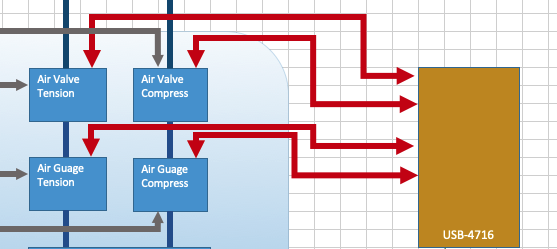
\includegraphics[width=3.12500in]{jira_imgs/3435.png}

}
\hdashrule[0.5ex]{\textwidth}{1pt}{3mm}
  Expected Result \\
{\footnotesize
The air valves and gauges are hooked up to the USB-4716 readout device.~

}
\hdashrule[0.5ex]{\textwidth}{1pt}{3mm}
  Actual Result \\
{\footnotesize

}
\begin{tabular}{p{2cm}p{14cm}}
\toprule
Step 6 & Step Execution Status: \textbf{ Not Executed } \\ \hline
\end{tabular}
 Description \\
{\footnotesize
Make the connection between the MB5U readout electronics and the
renishaw encoders.

}
\hdashrule[0.5ex]{\textwidth}{1pt}{3mm}
  Expected Result \\
{\footnotesize
The MB5U readouts are connected to the encoders.

}
\hdashrule[0.5ex]{\textwidth}{1pt}{3mm}
  Actual Result \\
{\footnotesize

}
\begin{tabular}{p{2cm}p{14cm}}
\toprule
Step 7 & Step Execution Status: \textbf{ Not Executed } \\ \hline
\end{tabular}
 Description \\
{\footnotesize
Make the connection between the 9150 load cell readout electronic and
the load cell.

}
\hdashrule[0.5ex]{\textwidth}{1pt}{3mm}
  Expected Result \\
{\footnotesize
The load cell is connected to the load cell readout electronic.

}
\hdashrule[0.5ex]{\textwidth}{1pt}{3mm}
  Actual Result \\
{\footnotesize

}
\begin{tabular}{p{2cm}p{14cm}}
\toprule
Step 8 & Step Execution Status: \textbf{ Not Executed } \\ \hline
\end{tabular}
 Description \\
{\footnotesize
Make the connection between the Hexapod Actuator to the thermal
scanner.~

}
\hdashrule[0.5ex]{\textwidth}{1pt}{3mm}
  Expected Result \\
{\footnotesize
The thermal scanner is connected to the hexapod actuator.

}
\hdashrule[0.5ex]{\textwidth}{1pt}{3mm}
  Actual Result \\
{\footnotesize

}
\begin{tabular}{p{2cm}p{14cm}}
\toprule
Step 9 & Step Execution Status: \textbf{ Not Executed } \\ \hline
\end{tabular}
 Description \\
{\footnotesize
Connect the following to the USB 3.0 Hub:

\begin{itemize}
\tightlist
\item
  (2) connections for MB5U Readout Electronic
\item
  USB-4716 Readout Device/Labjack T4
\item
  Temperature Readout
\item
  9150 Load Cell Readout Electronic
\end{itemize}

}
\hdashrule[0.5ex]{\textwidth}{1pt}{3mm}
  Expected Result \\
{\footnotesize
The USB 3.0 Hub is now connected to the readout electronics from the
previous steps.~

}
\hdashrule[0.5ex]{\textwidth}{1pt}{3mm}
  Actual Result \\
{\footnotesize

}
\begin{tabular}{p{2cm}p{14cm}}
\toprule
Step 10 & Step Execution Status: \textbf{ Not Executed } \\ \hline
\end{tabular}
 Description \\
{\footnotesize
Connect the laptop with LabVIEW software to the USB 3.0 Hub.

}
\hdashrule[0.5ex]{\textwidth}{1pt}{3mm}
  Expected Result \\
{\footnotesize
The Laptop is connected to the USB 3.0 Hub and to the subsequent readout
electronics.~

}
\hdashrule[0.5ex]{\textwidth}{1pt}{3mm}
  Actual Result \\
{\footnotesize

}
\begin{tabular}{p{2cm}p{14cm}}
\toprule
Step 11 & Step Execution Status: \textbf{ Not Executed } \\ \hline
\end{tabular}
 Description \\
{\footnotesize
Connect the laptop to the Copley Motor drive of the Control Box.

}
\hdashrule[0.5ex]{\textwidth}{1pt}{3mm}
  Expected Result \\
{\footnotesize
The laptop is connected to the control box.

}
\hdashrule[0.5ex]{\textwidth}{1pt}{3mm}
  Actual Result \\
{\footnotesize

}
\begin{tabular}{p{2cm}p{14cm}}
\toprule
Step 12 & Step Execution Status: \textbf{ Not Executed } \\ \hline
\end{tabular}
 Description \\
{\footnotesize
Set up the USB 3.0 Hub close to the test fixture and connect it to a
power source.~

}
\hdashrule[0.5ex]{\textwidth}{1pt}{3mm}
  Expected Result \\
{\footnotesize
The USB 3.0 Hub is connected and all readout devices are powered on.~

}
\hdashrule[0.5ex]{\textwidth}{1pt}{3mm}
  Actual Result \\
{\footnotesize

}
\begin{tabular}{p{2cm}p{14cm}}
\toprule
Step 13 & Step Execution Status: \textbf{ Not Executed } \\ \hline
\end{tabular}
 Description \\
{\footnotesize
Verify that the output data from the readout devices are available on
the laptop.

}
\hdashrule[0.5ex]{\textwidth}{1pt}{3mm}
  Expected Result \\
{\footnotesize
The laptop is seen to be able to communicate with the readout devices.

}
\hdashrule[0.5ex]{\textwidth}{1pt}{3mm}
  Actual Result \\
{\footnotesize

}
\begin{tabular}{p{2cm}p{14cm}}
\toprule
Step 14 & Step Execution Status: \textbf{ Not Executed } \\ \hline
\end{tabular}
 Description \\
{\footnotesize
Open Labview 2021 in the computer used for Test Setup.

}
\hdashrule[0.5ex]{\textwidth}{1pt}{3mm}
  Expected Result \\
{\footnotesize
Labview 2021 opens successfully.

}
\hdashrule[0.5ex]{\textwidth}{1pt}{3mm}
  Actual Result \\
{\footnotesize

}
\begin{tabular}{p{2cm}p{14cm}}
\toprule
Step 15 & Step Execution Status: \textbf{ Not Executed } \\ \hline
\end{tabular}
 Description \\
{\footnotesize
Open the Labview VI files from the project directory including sub VIs-
Tovey Closed loop.vi, Voltage Regulation.vi and Biss Reader.vi

}
\hdashrule[0.5ex]{\textwidth}{1pt}{3mm}
  Expected Result \\
{\footnotesize
Front panel of VI and sub VI files open without any error.

}
\hdashrule[0.5ex]{\textwidth}{1pt}{3mm}
  Actual Result \\
{\footnotesize

}
\begin{tabular}{p{2cm}p{14cm}}
\toprule
Step 16 & Step Execution Status: \textbf{ Not Executed } \\ \hline
\end{tabular}
 Description \\
{\footnotesize
Configure the Biss Reader.vi file with the appropriate configuration
file and following the IBISS operation manual.~

}
\hdashrule[0.5ex]{\textwidth}{1pt}{3mm}
  Expected Result \\
{\footnotesize
\href{https://jira.lsstcorp.org/rest/tests/1.0/attachment/3555}{BiSS\_config.cfg}
is loaded in the LabView configuration (Misc Tab under Load DLL). The
configuration file is based on the IBISS operation manual.

}
\hdashrule[0.5ex]{\textwidth}{1pt}{3mm}
  Actual Result \\
{\footnotesize

}
\begin{tabular}{p{2cm}p{14cm}}
\toprule
Step 17 & Step Execution Status: \textbf{ Not Executed } \\ \hline
\end{tabular}
 Description \\
{\footnotesize
Click Run button on the on the block diagram toolbar of the Labview VI
front panel.

}
\hdashrule[0.5ex]{\textwidth}{1pt}{3mm}
  Expected Result \\
{\footnotesize
LabView VI and ~associated sub Vi runs successfully. Initially all the
graphs and input values will be blank.

}
\hdashrule[0.5ex]{\textwidth}{1pt}{3mm}
  Actual Result \\
{\footnotesize

}
\begin{tabular}{p{2cm}p{14cm}}
\toprule
Step 18 & Step Execution Status: \textbf{ Not Executed } \\ \hline
\end{tabular}
 Description \\
{\footnotesize
Send a command through LabVIEW ~voltage Regulation.vi to set the voltage
on the compression valve only to 3V.

}
\hdashrule[0.5ex]{\textwidth}{1pt}{3mm}
  Expected Result \\
{\footnotesize
The command is accepted, the pneumatic valve shows the applied voltage
only on the compression valve and the applied compression force can be
seen on the LabView front panel Time vs Load graph.~

}
\hdashrule[0.5ex]{\textwidth}{1pt}{3mm}
  Actual Result \\
{\footnotesize

}
\begin{tabular}{p{2cm}p{14cm}}
\toprule
Step 19 & Step Execution Status: \textbf{ Not Executed } \\ \hline
\end{tabular}
 Description \\
{\footnotesize
Send a command through LabVIEW voltage Regulation.vi to reset the
compression valve to 0V.

}
\hdashrule[0.5ex]{\textwidth}{1pt}{3mm}
  Expected Result \\
{\footnotesize
The command is accepted. The applied force can be seen as zero load on
the LabView front panel Time vs Load graph. Load Cell Reader also shows
zero load.

}
\hdashrule[0.5ex]{\textwidth}{1pt}{3mm}
  Actual Result \\
{\footnotesize

}
\begin{tabular}{p{2cm}p{14cm}}
\toprule
Step 20 & Step Execution Status: \textbf{ Not Executed } \\ \hline
\end{tabular}
 Description \\
{\footnotesize
Send a command through LabVIEW to reset the tension valve to 3V.

}
\hdashrule[0.5ex]{\textwidth}{1pt}{3mm}
  Expected Result \\
{\footnotesize
The command is accepted, the readout electronic shows the applied
voltage only on the tension valve and the applied tension force can be
seen on the LabView front panel Time vs Load graph.

}
\hdashrule[0.5ex]{\textwidth}{1pt}{3mm}
  Actual Result \\
{\footnotesize

}
\begin{tabular}{p{2cm}p{14cm}}
\toprule
Step 21 & Step Execution Status: \textbf{ Not Executed } \\ \hline
\end{tabular}
 Description \\
{\footnotesize
Send a command through LabVIEW to reset the tension valve to 0V.

}
\hdashrule[0.5ex]{\textwidth}{1pt}{3mm}
  Expected Result \\
{\footnotesize
The command is accepted, the readout electronic no longer shows the
applied voltage on the tension valve and there is no longer any tension
force on the LabView front panel Time vs Load graph.

}
\hdashrule[0.5ex]{\textwidth}{1pt}{3mm}
  Actual Result \\
{\footnotesize

}
\begin{tabular}{p{2cm}p{14cm}}
\toprule
Step 22 & Step Execution Status: \textbf{ Not Executed } \\ \hline
\end{tabular}
 Description \\
{\footnotesize
Verify the laptop is reading the renishaw scales usinthe Biss Reader.vi
file and determine the zero stroke position.

}
\hdashrule[0.5ex]{\textwidth}{1pt}{3mm}
  Test Data \\
 {\footnotesize
\textbf{Note:~}Moog's original test procedure cited the zero position to
be at 40mm since the full length was 80mm.

}
\hdashrule[0.5ex]{\textwidth}{1pt}{3mm}
  Expected Result \\
{\footnotesize
40mm encoder readings shown in Labview front panel of the .vi file.~\\
The zero stroke position has been determined and can be used as a
reference for the offset of future moves.

}
\hdashrule[0.5ex]{\textwidth}{1pt}{3mm}
  Actual Result \\
{\footnotesize

}

\paragraph{ LVV-T2428 - Hexapod - Actuator Stiffness Test }\mbox{}\\

Version \textbf{1}.
Status \textbf{Approved}.
Open  \href{https://jira.lsstcorp.org/secure/Tests.jspa#/testCase/LVV-T2428}{\textit{ LVV-T2428 } }
test case in Jira.



\textbf{ Preconditions}:\\


Execution status: {\bf Not Executed }

Final comment:\\


Detailed steps results:

\begin{tabular}{p{2cm}p{14cm}}
\toprule
Step 1 & Step Execution Status: \textbf{ Not Executed } \\ \hline
\end{tabular}
 Description \\
{\footnotesize
Open Labview 2021 in the computer used for Test Setup.

}
\hdashrule[0.5ex]{\textwidth}{1pt}{3mm}
  Test Data \\
 {\footnotesize
\textbf{Note:~}The first three steps are conditional because these steps
are included as part of the Test Setup procedure and may not be
necessary if LabView is still open.

}
\hdashrule[0.5ex]{\textwidth}{1pt}{3mm}
  Expected Result \\
{\footnotesize
Labview 2021 opens successfully.

}
\hdashrule[0.5ex]{\textwidth}{1pt}{3mm}
  Actual Result \\
{\footnotesize

}
\begin{tabular}{p{2cm}p{14cm}}
\toprule
Step 2 & Step Execution Status: \textbf{ Not Executed } \\ \hline
\end{tabular}
 Description \\
{\footnotesize
Open Labview 2021 in the computer used for Test Setup.

}
\hdashrule[0.5ex]{\textwidth}{1pt}{3mm}
  Test Data \\
 {\footnotesize
\textbf{Note:~}The first three steps are conditional because these steps
are included as part of the Test Setup procedure and may not be
necessary if LabView is still open.

}
\hdashrule[0.5ex]{\textwidth}{1pt}{3mm}
  Expected Result \\
{\footnotesize
Labview 2021 opens successfully.

}
\hdashrule[0.5ex]{\textwidth}{1pt}{3mm}
  Actual Result \\
{\footnotesize

}
\begin{tabular}{p{2cm}p{14cm}}
\toprule
Step 3 & Step Execution Status: \textbf{ Not Executed } \\ \hline
\end{tabular}
 Description \\
{\footnotesize
Open the Labview VI files from the project directory including sub VIs-
Tovey Closed loop.vi, Voltage Regulation.vi and Biss Reader.vi

}
\hdashrule[0.5ex]{\textwidth}{1pt}{3mm}
  Expected Result \\
{\footnotesize
Front panel of VI and sub VI files open without any error.

}
\hdashrule[0.5ex]{\textwidth}{1pt}{3mm}
  Actual Result \\
{\footnotesize

}
\begin{tabular}{p{2cm}p{14cm}}
\toprule
Step 4 & Step Execution Status: \textbf{ Not Executed } \\ \hline
\end{tabular}
 Description \\
{\footnotesize
Open the Labview VI files from the project directory including sub VIs-
Tovey Closed loop.vi, Voltage Regulation.vi and Biss Reader.vi

}
\hdashrule[0.5ex]{\textwidth}{1pt}{3mm}
  Expected Result \\
{\footnotesize
Front panel of VI and sub VI files open without any error.

}
\hdashrule[0.5ex]{\textwidth}{1pt}{3mm}
  Actual Result \\
{\footnotesize

}
\begin{tabular}{p{2cm}p{14cm}}
\toprule
Step 5 & Step Execution Status: \textbf{ Not Executed } \\ \hline
\end{tabular}
 Description \\
{\footnotesize
Click Run button on the on the block diagram toolbar of the Labview VI
front panel.

}
\hdashrule[0.5ex]{\textwidth}{1pt}{3mm}
  Expected Result \\
{\footnotesize
LabView VI and ~associated sub Vi runs successfully. Initially all the
graphs and input values will be blank.

}
\hdashrule[0.5ex]{\textwidth}{1pt}{3mm}
  Actual Result \\
{\footnotesize

}
\begin{tabular}{p{2cm}p{14cm}}
\toprule
Step 6 & Step Execution Status: \textbf{ Not Executed } \\ \hline
\end{tabular}
 Description \\
{\footnotesize
Click Run button on the on the block diagram toolbar of the Labview VI
front panel.

}
\hdashrule[0.5ex]{\textwidth}{1pt}{3mm}
  Expected Result \\
{\footnotesize
LabView VI and ~associated sub Vi runs successfully. Initially all the
graphs and input values will be blank.

}
\hdashrule[0.5ex]{\textwidth}{1pt}{3mm}
  Actual Result \\
{\footnotesize

}
\begin{tabular}{p{2cm}p{14cm}}
\toprule
Step 7 & Step Execution Status: \textbf{ Not Executed } \\ \hline
\end{tabular}
 Description \\
{\footnotesize
Position the actuator at its center of stroke.

}
\hdashrule[0.5ex]{\textwidth}{1pt}{3mm}
  Test Data \\
 {\footnotesize
\textbf{Note:~}The original zero position/center of stroke position was
determined to be a linear encoder reading of 40mm. For the purpose of
this test, the same center of stroke position will be used.

}
\hdashrule[0.5ex]{\textwidth}{1pt}{3mm}
  Expected Result \\
{\footnotesize
Actuator positioned at its center of stroke position ~confirmed by
encoder reading in the LabView.\\[2\baselineskip]

}
\hdashrule[0.5ex]{\textwidth}{1pt}{3mm}
  Actual Result \\
{\footnotesize

}
\begin{tabular}{p{2cm}p{14cm}}
\toprule
Step 8 & Step Execution Status: \textbf{ Not Executed } \\ \hline
\end{tabular}
 Description \\
{\footnotesize
Position the actuator at its center of stroke.

}
\hdashrule[0.5ex]{\textwidth}{1pt}{3mm}
  Test Data \\
 {\footnotesize
\textbf{Note:~}The original zero position/center of stroke position was
determined to be a linear encoder reading of 40mm. For the purpose of
this test, the same center of stroke position will be used.

}
\hdashrule[0.5ex]{\textwidth}{1pt}{3mm}
  Expected Result \\
{\footnotesize
Actuator positioned at its center of stroke position ~confirmed by
encoder reading in the LabView.\\[2\baselineskip]

}
\hdashrule[0.5ex]{\textwidth}{1pt}{3mm}
  Actual Result \\
{\footnotesize

}
\begin{tabular}{p{2cm}p{14cm}}
\toprule
Step 9 & Step Execution Status: \textbf{ Not Executed } \\ \hline
\end{tabular}
 Description \\
{\footnotesize
Disable Motor Power by pressing the Emergency stop button on the control
box.

}
\hdashrule[0.5ex]{\textwidth}{1pt}{3mm}
  Expected Result \\
{\footnotesize
Motor power disabled.

}
\hdashrule[0.5ex]{\textwidth}{1pt}{3mm}
  Actual Result \\
{\footnotesize

}
\begin{tabular}{p{2cm}p{14cm}}
\toprule
Step 10 & Step Execution Status: \textbf{ Not Executed } \\ \hline
\end{tabular}
 Description \\
{\footnotesize
Disable Motor Power by pressing the Emergency stop button on the control
box.

}
\hdashrule[0.5ex]{\textwidth}{1pt}{3mm}
  Expected Result \\
{\footnotesize
Motor power disabled.

}
\hdashrule[0.5ex]{\textwidth}{1pt}{3mm}
  Actual Result \\
{\footnotesize

}
\begin{tabular}{p{2cm}p{14cm}}
\toprule
Step 11 & Step Execution Status: \textbf{ Not Executed } \\ \hline
\end{tabular}
 Description \\
{\footnotesize
Iteration {1}⁠ : Increase the load on the actuator from 0 kN to
approximately 30kN (6744 lbf) tension

}
\hdashrule[0.5ex]{\textwidth}{1pt}{3mm}
  Test Data \\
 {\footnotesize
\textbf{Note:~}In order to apply a tension force of 30 KN:

\begin{itemize}
\tightlist
\item
  Set pneumatic valve (closest to hexapod actuator side) to 3.5V (0-10
  Vdc) while the other valve remains at 0V.
\item
  increase air supply using LabVIEW function~
\end{itemize}

}
\hdashrule[0.5ex]{\textwidth}{1pt}{3mm}
  Expected Result \\
{\footnotesize
Load cell reader shows the applied 30 KN tension force.\\
LabView displays the voltage being applied.

}
\hdashrule[0.5ex]{\textwidth}{1pt}{3mm}
  Actual Result \\
{\footnotesize

}
\begin{tabular}{p{2cm}p{14cm}}
\toprule
Step 12 & Step Execution Status: \textbf{ Not Executed } \\ \hline
\end{tabular}
 Description \\
{\footnotesize
Iteration {2}⁠ : Increase the load on the actuator from 0 kN to
approximately 30kN (6744 lbf) tension

}
\hdashrule[0.5ex]{\textwidth}{1pt}{3mm}
  Test Data \\
 {\footnotesize
\textbf{Note:~}In order to apply a tension force of 30 KN:

\begin{itemize}
\tightlist
\item
  Set pneumatic valve (closest to hexapod actuator side) to 3.5V (0-10
  Vdc) while the other valve remains at 0V.
\item
  increase air supply using LabVIEW function~
\end{itemize}

}
\hdashrule[0.5ex]{\textwidth}{1pt}{3mm}
  Expected Result \\
{\footnotesize
Load cell reader shows the applied 30 KN tension force.\\
LabView displays the voltage being applied.

}
\hdashrule[0.5ex]{\textwidth}{1pt}{3mm}
  Actual Result \\
{\footnotesize

}
\begin{tabular}{p{2cm}p{14cm}}
\toprule
Step 13 & Step Execution Status: \textbf{ Not Executed } \\ \hline
\end{tabular}
 Description \\
{\footnotesize
Iteration {{1}⁠} :Reduce the load through zero load to approximately 30
kN (6744 lbf) compression, and return to zero load.

}
\hdashrule[0.5ex]{\textwidth}{1pt}{3mm}
  Test Data \\
 {\footnotesize
\textbf{Note:~}In order to apply a compression force of 30kN:\\

\begin{itemize}
\tightlist
\item
  Set pneumatic valve (far from the hexapod actuator side) to 3.5V (0-10
  Vdc) while the other valve remains at 0V ( reverse from step 6).
\item
  increase air supply using LabVIEW function~
\end{itemize}

}
\hdashrule[0.5ex]{\textwidth}{1pt}{3mm}
  Expected Result \\
{\footnotesize
Load graphs shows the fluctuation of loads from 30 KN tension to zero to
30 KN compression and back to zero load in LabView.~

}
\hdashrule[0.5ex]{\textwidth}{1pt}{3mm}
  Actual Result \\
{\footnotesize

}
\begin{tabular}{p{2cm}p{14cm}}
\toprule
Step 14 & Step Execution Status: \textbf{ Not Executed } \\ \hline
\end{tabular}
 Description \\
{\footnotesize
Iteration {{2}⁠} :Reduce the load through zero load to approximately 30
kN (6744 lbf) compression, and return to zero load.

}
\hdashrule[0.5ex]{\textwidth}{1pt}{3mm}
  Test Data \\
 {\footnotesize
\textbf{Note:~}In order to apply a compression force of 30kN:\\

\begin{itemize}
\tightlist
\item
  Set pneumatic valve (far from the hexapod actuator side) to 3.5V (0-10
  Vdc) while the other valve remains at 0V ( reverse from step 6).
\item
  increase air supply using LabVIEW function~
\end{itemize}

}
\hdashrule[0.5ex]{\textwidth}{1pt}{3mm}
  Expected Result \\
{\footnotesize
Load graphs shows the fluctuation of loads from 30 KN tension to zero to
30 KN compression and back to zero load in LabView.~

}
\hdashrule[0.5ex]{\textwidth}{1pt}{3mm}
  Actual Result \\
{\footnotesize

}
\begin{tabular}{p{2cm}p{14cm}}
\toprule
Step 15 & Step Execution Status: \textbf{ Not Executed } \\ \hline
\end{tabular}
 Description \\
{\footnotesize
Record the actual displacement as measured by the two external encoders
as LabView graph ( Time vs Displacement).\\[2\baselineskip]

}
\hdashrule[0.5ex]{\textwidth}{1pt}{3mm}
  Expected Result \\
{\footnotesize
Actual displacement measured by the average of the two external encoders
~recorded in the LabView graph.

}
\hdashrule[0.5ex]{\textwidth}{1pt}{3mm}
  Actual Result \\
{\footnotesize

}
\begin{tabular}{p{2cm}p{14cm}}
\toprule
Step 16 & Step Execution Status: \textbf{ Not Executed } \\ \hline
\end{tabular}
 Description \\
{\footnotesize
Record the actual displacement as measured by the two external encoders
as LabView graph ( Time vs Displacement).\\[2\baselineskip]

}
\hdashrule[0.5ex]{\textwidth}{1pt}{3mm}
  Expected Result \\
{\footnotesize
Actual displacement measured by the average of the two external encoders
~recorded in the LabView graph.

}
\hdashrule[0.5ex]{\textwidth}{1pt}{3mm}
  Actual Result \\
{\footnotesize

}
\begin{tabular}{p{2cm}p{14cm}}
\toprule
Step 17 & Step Execution Status: \textbf{ Not Executed } \\ \hline
\end{tabular}
 Description \\
{\footnotesize
View the a force vs displacement plot in the Labview.~\\[2\baselineskip]

}
\hdashrule[0.5ex]{\textwidth}{1pt}{3mm}
  Expected Result \\
{\footnotesize
The expected actuator stiffness is \textgreater{}= 134 N/um at center
stroke.~\\[2\baselineskip]

}
\hdashrule[0.5ex]{\textwidth}{1pt}{3mm}
  Actual Result \\
{\footnotesize

}
\begin{tabular}{p{2cm}p{14cm}}
\toprule
Step 18 & Step Execution Status: \textbf{ Not Executed } \\ \hline
\end{tabular}
 Description \\
{\footnotesize
View the a force vs displacement plot in the Labview.~\\[2\baselineskip]

}
\hdashrule[0.5ex]{\textwidth}{1pt}{3mm}
  Expected Result \\
{\footnotesize
The expected actuator stiffness is \textgreater{}= 134 N/um at center
stroke.~\\[2\baselineskip]

}
\hdashrule[0.5ex]{\textwidth}{1pt}{3mm}
  Actual Result \\
{\footnotesize

}
\begin{tabular}{p{2cm}p{14cm}}
\toprule
Step 19 & Step Execution Status: \textbf{ Not Executed } \\ \hline
\end{tabular}
 Description \\
{\footnotesize
Check if all the test results are recorded in excel spreadsheets.

}
\hdashrule[0.5ex]{\textwidth}{1pt}{3mm}
  Expected Result \\
{\footnotesize
Test Results are recorded in the excel spreadsheets residing in the
LabView Folder directory.

}
\hdashrule[0.5ex]{\textwidth}{1pt}{3mm}
  Actual Result \\
{\footnotesize

}
\begin{tabular}{p{2cm}p{14cm}}
\toprule
Step 20 & Step Execution Status: \textbf{ Not Executed } \\ \hline
\end{tabular}
 Description \\
{\footnotesize
Check if all the test results are recorded in excel spreadsheets.

}
\hdashrule[0.5ex]{\textwidth}{1pt}{3mm}
  Expected Result \\
{\footnotesize
Test Results are recorded in the excel spreadsheets residing in the
LabView Folder directory.

}
\hdashrule[0.5ex]{\textwidth}{1pt}{3mm}
  Actual Result \\
{\footnotesize

}
\begin{tabular}{p{2cm}p{14cm}}
\toprule
Step 21 & Step Execution Status: \textbf{ Not Executed } \\ \hline
\end{tabular}
 Description \\
{\footnotesize
Close all the Labview VI files.

}
\hdashrule[0.5ex]{\textwidth}{1pt}{3mm}
  Test Data \\
 {\footnotesize
\textbf{Note:~}Labview can be left open in order to continue to the next
test. However, it may be necessary to reset the application before
starting the next test.

}
\hdashrule[0.5ex]{\textwidth}{1pt}{3mm}
  Expected Result \\
{\footnotesize
All the VI files are closed and Labview 2021 application window closes.

}
\hdashrule[0.5ex]{\textwidth}{1pt}{3mm}
  Actual Result \\
{\footnotesize

}
\begin{tabular}{p{2cm}p{14cm}}
\toprule
Step 22 & Step Execution Status: \textbf{ Not Executed } \\ \hline
\end{tabular}
 Description \\
{\footnotesize
Close all the Labview VI files.

}
\hdashrule[0.5ex]{\textwidth}{1pt}{3mm}
  Test Data \\
 {\footnotesize
\textbf{Note:~}Labview can be left open in order to continue to the next
test. However, it may be necessary to reset the application before
starting the next test.

}
\hdashrule[0.5ex]{\textwidth}{1pt}{3mm}
  Expected Result \\
{\footnotesize
All the VI files are closed and Labview 2021 application window closes.

}
\hdashrule[0.5ex]{\textwidth}{1pt}{3mm}
  Actual Result \\
{\footnotesize

}

\paragraph{ LVV-T2432 - Hexapod - Actuator Range of Motion Test }\mbox{}\\

Version \textbf{1}.
Status \textbf{Approved}.
Open  \href{https://jira.lsstcorp.org/secure/Tests.jspa#/testCase/LVV-T2432}{\textit{ LVV-T2432 } }
test case in Jira.

To verify that the range of motions for the actuators stay within the
determined limits.

\textbf{ Preconditions}:\\
The range limits should be determined to achieve the camera hexapod's
simultaneous range of motion requirements.

Execution status: {\bf Not Executed }

Final comment:\\


Detailed steps results:

\begin{tabular}{p{2cm}p{14cm}}
\toprule
Step 1 & Step Execution Status: \textbf{ Not Executed } \\ \hline
\end{tabular}
 Description \\
{\footnotesize
Open Labview 2021 in the computer used for Test Setup.

}
\hdashrule[0.5ex]{\textwidth}{1pt}{3mm}
  Test Data \\
 {\footnotesize
The first three steps are conditional because these steps are included
as part of the Test Setup procedure and may not be necessary if LabView
is still open.\\[3\baselineskip]

}
\hdashrule[0.5ex]{\textwidth}{1pt}{3mm}
  Expected Result \\
{\footnotesize
Labview 2021 opens successfully.

}
\hdashrule[0.5ex]{\textwidth}{1pt}{3mm}
  Actual Result \\
{\footnotesize

}
\begin{tabular}{p{2cm}p{14cm}}
\toprule
Step 2 & Step Execution Status: \textbf{ Not Executed } \\ \hline
\end{tabular}
 Description \\
{\footnotesize
Open the Labview Biss Reader.vi file.~

}
\hdashrule[0.5ex]{\textwidth}{1pt}{3mm}
  Expected Result \\
{\footnotesize
Front panel of the VI a file open without any error.

}
\hdashrule[0.5ex]{\textwidth}{1pt}{3mm}
  Actual Result \\
{\footnotesize

}
\begin{tabular}{p{2cm}p{14cm}}
\toprule
Step 3 & Step Execution Status: \textbf{ Not Executed } \\ \hline
\end{tabular}
 Description \\
{\footnotesize
Click Run button on the on the block diagram toolbar of the Labview VI
front panel.

}
\hdashrule[0.5ex]{\textwidth}{1pt}{3mm}
  Expected Result \\
{\footnotesize
Biss Reader.vi run successfully. Initially all the graphs and input
values will be blank.

}
\hdashrule[0.5ex]{\textwidth}{1pt}{3mm}
  Actual Result \\
{\footnotesize

}
\begin{tabular}{p{2cm}p{14cm}}
\toprule
Step 4 & Step Execution Status: \textbf{ Not Executed } \\ \hline
\end{tabular}
 Description \\
{\footnotesize
Set software actuator stroke limits using the copley software to +/-
14.00mm.

}
\hdashrule[0.5ex]{\textwidth}{1pt}{3mm}
  Expected Result \\
{\footnotesize
Software actuator stroke limits set to +/- 14.00mm.

}
\hdashrule[0.5ex]{\textwidth}{1pt}{3mm}
  Actual Result \\
{\footnotesize

}
\begin{tabular}{p{2cm}p{14cm}}
\toprule
Step 5 & Step Execution Status: \textbf{ Not Executed } \\ \hline
\end{tabular}
 Description \\
{\footnotesize
Move the actuator forward and backward to confirm that positive position
commands correspond to extensions of the actuator and negative position
commands correspond to retractions of the actuator. If not, flipped the
sign of the encoder readings in software.~\\[2\baselineskip]

}
\hdashrule[0.5ex]{\textwidth}{1pt}{3mm}
  Expected Result \\
{\footnotesize
Positive position commands correspond to extensions; Negative position
commands correspond to retractions of the actuator.~

}
\hdashrule[0.5ex]{\textwidth}{1pt}{3mm}
  Actual Result \\
{\footnotesize

}
\begin{tabular}{p{2cm}p{14cm}}
\toprule
Step 6 & Step Execution Status: \textbf{ Not Executed } \\ \hline
\end{tabular}
 Description \\
{\footnotesize
Set the motor drive to halt motion using the control box and copley
software if a limit switch is tripped.\\[3\baselineskip]

}
\hdashrule[0.5ex]{\textwidth}{1pt}{3mm}
  Expected Result \\
{\footnotesize
Motor drive set to halt position if a limit switch is tripped.~

}
\hdashrule[0.5ex]{\textwidth}{1pt}{3mm}
  Actual Result \\
{\footnotesize

}
\begin{tabular}{p{2cm}p{14cm}}
\toprule
Step 7 & Step Execution Status: \textbf{ Not Executed } \\ \hline
\end{tabular}
 Description \\
{\footnotesize
Extend the actuator to its position stroke limit of +14mm using the
copley software and the~ control box.

}
\hdashrule[0.5ex]{\textwidth}{1pt}{3mm}
  Expected Result \\
{\footnotesize
Actuator extended to its position stroke limit of +14mm.

}
\hdashrule[0.5ex]{\textwidth}{1pt}{3mm}
  Actual Result \\
{\footnotesize

}
\begin{tabular}{p{2cm}p{14cm}}
\toprule
Step 8 & Step Execution Status: \textbf{ Not Executed } \\ \hline
\end{tabular}
 Description \\
{\footnotesize
Ensure that the actuator reaches this position without hitting the
mechanical end stop or extension limit switch.

}
\hdashrule[0.5ex]{\textwidth}{1pt}{3mm}
  Expected Result \\
{\footnotesize
Encoder reading in LabView shows that actuator reached the position.~\\
Mechanical End Stop/Extension Limit switch not hit.

}
\hdashrule[0.5ex]{\textwidth}{1pt}{3mm}
  Actual Result \\
{\footnotesize

}
\begin{tabular}{p{2cm}p{14cm}}
\toprule
Step 9 & Step Execution Status: \textbf{ Not Executed } \\ \hline
\end{tabular}
 Description \\
{\footnotesize
If the extension limit switch is contacted, the extension limit switch
position will need to be adjusted to be greater than 14mm and then the
try to extend the actuator to the position stroke limit of +14mm using
copley software and the control box.

}
\hdashrule[0.5ex]{\textwidth}{1pt}{3mm}
  Expected Result \\
{\footnotesize
Extension Limit Switch position readjusted and extended to the position
stroke limit of +14mm.

}
\hdashrule[0.5ex]{\textwidth}{1pt}{3mm}
  Actual Result \\
{\footnotesize

}
\begin{tabular}{p{2cm}p{14cm}}
\toprule
Step 10 & Step Execution Status: \textbf{ Not Executed } \\ \hline
\end{tabular}
 Description \\
{\footnotesize
Ensure that the actuator reaches this position without hitting the
mechanical end stop or extension limit switch.

}
\hdashrule[0.5ex]{\textwidth}{1pt}{3mm}
  Expected Result \\
{\footnotesize
Encoder reading in LabView shows that actuator reached the position.\\
Mechanical End Stop/Extension Limit switch not hit.

}
\hdashrule[0.5ex]{\textwidth}{1pt}{3mm}
  Actual Result \\
{\footnotesize

}
\begin{tabular}{p{2cm}p{14cm}}
\toprule
Step 11 & Step Execution Status: \textbf{ Not Executed } \\ \hline
\end{tabular}
 Description \\
{\footnotesize
Move the extension actuator stroke limit using the copley software to
+15.00mm .

}
\hdashrule[0.5ex]{\textwidth}{1pt}{3mm}
  Expected Result \\
{\footnotesize
Extension actuator stroke limit moved to +15.00mm.~

}
\hdashrule[0.5ex]{\textwidth}{1pt}{3mm}
  Actual Result \\
{\footnotesize

}
\begin{tabular}{p{2cm}p{14cm}}
\toprule
Step 12 & Step Execution Status: \textbf{ Not Executed } \\ \hline
\end{tabular}
 Description \\
{\footnotesize
Extend the actuator at maximum velocity until the extension limit switch
is actuated.

}
\hdashrule[0.5ex]{\textwidth}{1pt}{3mm}
  Test Data \\
 {\footnotesize
\textbf{Note:~}The maximum velocity is +/-0.5mm/s

}
\hdashrule[0.5ex]{\textwidth}{1pt}{3mm}
  Expected Result \\
{\footnotesize
Actuator extended at maximum velocity until the extension limit switch
is actuated.~

}
\hdashrule[0.5ex]{\textwidth}{1pt}{3mm}
  Actual Result \\
{\footnotesize

}
\begin{tabular}{p{2cm}p{14cm}}
\toprule
Step 13 & Step Execution Status: \textbf{ Not Executed } \\ \hline
\end{tabular}
 Description \\
{\footnotesize
If the actuator hits the stroke limit before tripping the limit switch
or appears to contact the end stop after tripping the limit switch
(before it can stop), reposition the limit switch. Then, repeat test
using copley software and the control box.\\[2\baselineskip]

}
\hdashrule[0.5ex]{\textwidth}{1pt}{3mm}
  Expected Result \\
{\footnotesize
Limit switch repositioned and extended the actuator to the position
stroke limit of +15mm.~

}
\hdashrule[0.5ex]{\textwidth}{1pt}{3mm}
  Actual Result \\
{\footnotesize

}
\begin{tabular}{p{2cm}p{14cm}}
\toprule
Step 14 & Step Execution Status: \textbf{ Not Executed } \\ \hline
\end{tabular}
 Description \\
{\footnotesize
Record the final position of the limit switch.~\\[2\baselineskip]

}
\hdashrule[0.5ex]{\textwidth}{1pt}{3mm}
  Expected Result \\
{\footnotesize
\textbf{Final position of the limit switch around +14.50mm.}

}
\hdashrule[0.5ex]{\textwidth}{1pt}{3mm}
  Actual Result \\
{\footnotesize

}
\begin{tabular}{p{2cm}p{14cm}}
\toprule
Step 15 & Step Execution Status: \textbf{ Not Executed } \\ \hline
\end{tabular}
 Description \\
{\footnotesize
Repeat the steps 6-14 two more times to assess limit switch position
repeatability. ~\\[3\baselineskip]

}
\hdashrule[0.5ex]{\textwidth}{1pt}{3mm}
  Expected Result \\
{\footnotesize
Final positions of the limit switch close to step 14 result(Around
+14.50).

}
\hdashrule[0.5ex]{\textwidth}{1pt}{3mm}
  Actual Result \\
{\footnotesize

}
\begin{tabular}{p{2cm}p{14cm}}
\toprule
Step 16 & Step Execution Status: \textbf{ Not Executed } \\ \hline
\end{tabular}
 Description \\
{\footnotesize
Retract the actuator to its position stroke limit of -14 mm using the
copley software and the ~control box.\\[2\baselineskip]

}
\hdashrule[0.5ex]{\textwidth}{1pt}{3mm}
  Expected Result \\
{\footnotesize
Actuator retracted to its position stroke limit of -14.04mm.

}
\hdashrule[0.5ex]{\textwidth}{1pt}{3mm}
  Actual Result \\
{\footnotesize

}
\begin{tabular}{p{2cm}p{14cm}}
\toprule
Step 17 & Step Execution Status: \textbf{ Not Executed } \\ \hline
\end{tabular}
 Description \\
{\footnotesize
Ensure that the actuator reaches this position without hitting the
mechanical end stop or retraction limit switch.

}
\hdashrule[0.5ex]{\textwidth}{1pt}{3mm}
  Expected Result \\
{\footnotesize
Encoder reading in LabView shows that actuator reached the position.\\
Mechanical End Stop/Retraction Limit switch not hit.

}
\hdashrule[0.5ex]{\textwidth}{1pt}{3mm}
  Actual Result \\
{\footnotesize

}
\begin{tabular}{p{2cm}p{14cm}}
\toprule
Step 18 & Step Execution Status: \textbf{ Not Executed } \\ \hline
\end{tabular}
 Description \\
{\footnotesize
If the retraction limit switch is contacted, the retraction limit switch
position will need to be adjusted to be greater than -14mm and then the
try to retract the actuator to the position stroke limit of -14mm using
copley software and the control box.

}
\hdashrule[0.5ex]{\textwidth}{1pt}{3mm}
  Expected Result \\
{\footnotesize
Retraction limit switch position readjusted and the actuator retracted
to the position stroke limit of -14mm.

}
\hdashrule[0.5ex]{\textwidth}{1pt}{3mm}
  Actual Result \\
{\footnotesize

}
\begin{tabular}{p{2cm}p{14cm}}
\toprule
Step 19 & Step Execution Status: \textbf{ Not Executed } \\ \hline
\end{tabular}
 Description \\
{\footnotesize
Ensure that the actuator reaches this position without hitting the
mechanical end stop or retraction limit switch.

}
\hdashrule[0.5ex]{\textwidth}{1pt}{3mm}
  Expected Result \\
{\footnotesize
Encoder reading in LabView shows that actuator reached the position.\\
Mechanical End Stop/Retraction Limit switch not hit.

}
\hdashrule[0.5ex]{\textwidth}{1pt}{3mm}
  Actual Result \\
{\footnotesize

}
\begin{tabular}{p{2cm}p{14cm}}
\toprule
Step 20 & Step Execution Status: \textbf{ Not Executed } \\ \hline
\end{tabular}
 Description \\
{\footnotesize
Move the retraction actuator stroke limit to -15.00mm .~

}
\hdashrule[0.5ex]{\textwidth}{1pt}{3mm}
  Expected Result \\
{\footnotesize
Retraction actuator stroke limit moved to -15.00mm.

}
\hdashrule[0.5ex]{\textwidth}{1pt}{3mm}
  Actual Result \\
{\footnotesize

}
\begin{tabular}{p{2cm}p{14cm}}
\toprule
Step 21 & Step Execution Status: \textbf{ Not Executed } \\ \hline
\end{tabular}
 Description \\
{\footnotesize
Retract the actuator at maximum velocity until the retraction limit
switch is actuated.

}
\hdashrule[0.5ex]{\textwidth}{1pt}{3mm}
  Test Data \\
 {\footnotesize
\textbf{Note:~}The maximum velocity is +/-0.5mm/s

}
\hdashrule[0.5ex]{\textwidth}{1pt}{3mm}
  Expected Result \\
{\footnotesize
Actuator retracted at maximum velocity until the retraction limit switch
is actuated.

}
\hdashrule[0.5ex]{\textwidth}{1pt}{3mm}
  Actual Result \\
{\footnotesize

}
\begin{tabular}{p{2cm}p{14cm}}
\toprule
Step 22 & Step Execution Status: \textbf{ Not Executed } \\ \hline
\end{tabular}
 Description \\
{\footnotesize
If the actuator hits the stroke limit before tripping the limit switch
or appears to contact the end stop after tripping the limit switch
(before it can stop), reposition the limit switch and repeat test.

}
\hdashrule[0.5ex]{\textwidth}{1pt}{3mm}
  Expected Result \\
{\footnotesize
Limit switch repositioned and retracted the actuator to the position
stroke limit of -15mm.

}
\hdashrule[0.5ex]{\textwidth}{1pt}{3mm}
  Actual Result \\
{\footnotesize

}
\begin{tabular}{p{2cm}p{14cm}}
\toprule
Step 23 & Step Execution Status: \textbf{ Not Executed } \\ \hline
\end{tabular}
 Description \\
{\footnotesize
Record the final position of the limit switch.

}
\hdashrule[0.5ex]{\textwidth}{1pt}{3mm}
  Expected Result \\
{\footnotesize
\textbf{Final position of the limit switch around -14.50mm.}

}
\hdashrule[0.5ex]{\textwidth}{1pt}{3mm}
  Actual Result \\
{\footnotesize

}
\begin{tabular}{p{2cm}p{14cm}}
\toprule
Step 24 & Step Execution Status: \textbf{ Not Executed } \\ \hline
\end{tabular}
 Description \\
{\footnotesize
Repeat the steps 16-23 two more times to assess limit switch position
repeatability.

}
\hdashrule[0.5ex]{\textwidth}{1pt}{3mm}
  Expected Result \\
{\footnotesize
Final positions of the limit switch close to step 15 result(Around
-14.50).

}
\hdashrule[0.5ex]{\textwidth}{1pt}{3mm}
  Actual Result \\
{\footnotesize

}
\begin{tabular}{p{2cm}p{14cm}}
\toprule
Step 25 & Step Execution Status: \textbf{ Not Executed } \\ \hline
\end{tabular}
 Description \\
{\footnotesize
Check if all the test results are recorded in excel spreadsheets.

}
\hdashrule[0.5ex]{\textwidth}{1pt}{3mm}
  Expected Result \\
{\footnotesize
Test Results are recorded in the excel spreadsheets residing in the
LabView Folder directory.\\[2\baselineskip]

}
\hdashrule[0.5ex]{\textwidth}{1pt}{3mm}
  Actual Result \\
{\footnotesize

}
\begin{tabular}{p{2cm}p{14cm}}
\toprule
Step 26 & Step Execution Status: \textbf{ Not Executed } \\ \hline
\end{tabular}
 Description \\
{\footnotesize
Close the Labview Vi file.

}
\hdashrule[0.5ex]{\textwidth}{1pt}{3mm}
  Test Data \\
 {\footnotesize
\textbf{Note:~}Labview can be left open in order to continue to the next
test. However, it may be necessary to reset the application before
starting the next test.

}
\hdashrule[0.5ex]{\textwidth}{1pt}{3mm}
  Expected Result \\
{\footnotesize
Labview 2021 application window closes.

}
\hdashrule[0.5ex]{\textwidth}{1pt}{3mm}
  Actual Result \\
{\footnotesize

}

\paragraph{ LVV-T2437 - Hexapod - Actuator Movement Test }\mbox{}\\

Version \textbf{1}.
Status \textbf{Approved}.
Open  \href{https://jira.lsstcorp.org/secure/Tests.jspa#/testCase/LVV-T2437}{\textit{ LVV-T2437 } }
test case in Jira.

The purpose of this test will be to verify that the actuators are able
to move within their velocity and acceleration limits. Furthermore,
during the moves, we will also be verifying that the actuators do not
take more than 2 seconds to settle into place.~

\textbf{ Preconditions}:\\


Execution status: {\bf Not Executed }

Final comment:\\


Detailed steps results:

\begin{tabular}{p{2cm}p{14cm}}
\toprule
Step 1 & Step Execution Status: \textbf{ Not Executed } \\ \hline
\end{tabular}
 Description \\
{\footnotesize
Open Labview 2021 in the computer used for Test Setup.

}
\hdashrule[0.5ex]{\textwidth}{1pt}{3mm}
  Test Data \\
 {\footnotesize
The first three steps are conditional because these steps are included
as part of the Test Setup procedure and may not be necessary if LabView
is still open.

}
\hdashrule[0.5ex]{\textwidth}{1pt}{3mm}
  Expected Result \\
{\footnotesize
Labview 2021 opens successfully.

}
\hdashrule[0.5ex]{\textwidth}{1pt}{3mm}
  Actual Result \\
{\footnotesize

}
\begin{tabular}{p{2cm}p{14cm}}
\toprule
Step 2 & Step Execution Status: \textbf{ Not Executed } \\ \hline
\end{tabular}
 Description \\
{\footnotesize
Open the Labview VI files from the project directory including sub VIs-
Tovey Closed loop.vi, Voltage Regulation.vi and Biss Reader.vi

}
\hdashrule[0.5ex]{\textwidth}{1pt}{3mm}
  Expected Result \\
{\footnotesize
Front panel of VI and sub VI files open without any error.

}
\hdashrule[0.5ex]{\textwidth}{1pt}{3mm}
  Actual Result \\
{\footnotesize

}
\begin{tabular}{p{2cm}p{14cm}}
\toprule
Step 3 & Step Execution Status: \textbf{ Not Executed } \\ \hline
\end{tabular}
 Description \\
{\footnotesize
Click Run button on the on the block diagram toolbar of the Labview VI
front panel.

}
\hdashrule[0.5ex]{\textwidth}{1pt}{3mm}
  Expected Result \\
{\footnotesize
LabView VI and ~associated sub Vi runs successfully. Initially all the
graphs and input values will be blank.

}
\hdashrule[0.5ex]{\textwidth}{1pt}{3mm}
  Actual Result \\
{\footnotesize

}
\begin{tabular}{p{2cm}p{14cm}}
\toprule
Step 4 & Step Execution Status: \textbf{ Not Executed } \\ \hline
\end{tabular}
 Description \\
{\footnotesize
Apply a 15kN compression load by using the LabView function to increase
the air supply value of \textasciitilde{}1.75V to one of the pneumatic
valve.

}
\hdashrule[0.5ex]{\textwidth}{1pt}{3mm}
  Test Data \\
 {\footnotesize
\begin{itemize}
\tightlist
\item
  Tension Load - Tension air Valve ( nearest one) will be set to 1.75V
  and other valve will be set to 0V. \textbf{~}{~~}
\end{itemize}

}
\hdashrule[0.5ex]{\textwidth}{1pt}{3mm}
  Expected Result \\
{\footnotesize
The LabView load graph( Time vs Load) shows 15 KN compression load
applied.

}
\hdashrule[0.5ex]{\textwidth}{1pt}{3mm}
  Actual Result \\
{\footnotesize

}
\begin{tabular}{p{2cm}p{14cm}}
\toprule
Step 5 & Step Execution Status: \textbf{ Not Executed } \\ \hline
\end{tabular}
 Description \\
{\footnotesize
Within the copley software, set the maximum actuator velocity to +/-0.5
mm/s.

}
\hdashrule[0.5ex]{\textwidth}{1pt}{3mm}
  Test Data \\
 {\footnotesize
\textbf{Note:~}This should be done by through the use of the command box
(pending instructions from Oli)

}
\hdashrule[0.5ex]{\textwidth}{1pt}{3mm}
  Expected Result \\
{\footnotesize
The maximum velocity is set to 0.5mm/s.

}
\hdashrule[0.5ex]{\textwidth}{1pt}{3mm}
  Actual Result \\
{\footnotesize

}
\begin{tabular}{p{2cm}p{14cm}}
\toprule
Step 6 & Step Execution Status: \textbf{ Not Executed } \\ \hline
\end{tabular}
 Description \\
{\footnotesize
Within the copley software, set the actuator acceleration and
deceleration limits to 0.5mm/s\^{}2.

}
\hdashrule[0.5ex]{\textwidth}{1pt}{3mm}
  Test Data \\
 {\footnotesize
\textbf{Note:~}This should be done by through the use of the command box
(pending instructions from Oli)

}
\hdashrule[0.5ex]{\textwidth}{1pt}{3mm}
  Expected Result \\
{\footnotesize
The maximum acceleration is set to 0.5mm/s\^{}2.

}
\hdashrule[0.5ex]{\textwidth}{1pt}{3mm}
  Actual Result \\
{\footnotesize

}
\begin{tabular}{p{2cm}p{14cm}}
\toprule
Step 7 & Step Execution Status: \textbf{ Not Executed } \\ \hline
\end{tabular}
 Description \\
{\footnotesize
Using the copley software, command the actuator to move 5mm.

}
\hdashrule[0.5ex]{\textwidth}{1pt}{3mm}
  Expected Result \\
{\footnotesize
The Labview graph (Time vs Position) shows the actuator travels 0.342mm
in 2 seconds or less.

}
\hdashrule[0.5ex]{\textwidth}{1pt}{3mm}
  Actual Result \\
{\footnotesize

}
\begin{tabular}{p{2cm}p{14cm}}
\toprule
Step 8 & Step Execution Status: \textbf{ Not Executed } \\ \hline
\end{tabular}
 Description \\
{\footnotesize
Verify the actuator does not move after reaching the commanded position
by checking the Labview graph (Time vs. Position).

}
\hdashrule[0.5ex]{\textwidth}{1pt}{3mm}
  Expected Result \\
{\footnotesize
The labview graph( Time vs Position) shows the actuator is no longer in
motion.

}
\hdashrule[0.5ex]{\textwidth}{1pt}{3mm}
  Actual Result \\
{\footnotesize

}
\begin{tabular}{p{2cm}p{14cm}}
\toprule
Step 9 & Step Execution Status: \textbf{ Not Executed } \\ \hline
\end{tabular}
 Description \\
{\footnotesize
Using the copley software, command the actuator to move 5mm in the
opposite direction, returning the original position.

}
\hdashrule[0.5ex]{\textwidth}{1pt}{3mm}
  Test Data \\
 {\footnotesize
\textbf{Note:~}Since the velocity or acceleration limits have not
changed, this should take the same amount of time.

}
\hdashrule[0.5ex]{\textwidth}{1pt}{3mm}
  Expected Result \\
{\footnotesize
The labview graph (Time vs Position) shows the actuator moves back 5mm
in less than 2 seconds.

}
\hdashrule[0.5ex]{\textwidth}{1pt}{3mm}
  Actual Result \\
{\footnotesize

}
\begin{tabular}{p{2cm}p{14cm}}
\toprule
Step 10 & Step Execution Status: \textbf{ Not Executed } \\ \hline
\end{tabular}
 Description \\
{\footnotesize
Now apply a 15kN tension load by using the LabView function to increase
the air supply value of \textasciitilde{}1.75V to other pneumatic valve.

}
\hdashrule[0.5ex]{\textwidth}{1pt}{3mm}
  Test Data \\
 {\footnotesize
\begin{itemize}
\tightlist
\item
  Compression Load - Compression air Valve ( Farthest one) will be set
  to 1.75V and other valve will be set to 0V.
\end{itemize}

}
\hdashrule[0.5ex]{\textwidth}{1pt}{3mm}
  Expected Result \\
{\footnotesize
The LabView load graph( Time vs Load) shows 15 KN tension load has been
applied.

}
\hdashrule[0.5ex]{\textwidth}{1pt}{3mm}
  Actual Result \\
{\footnotesize

}
\begin{tabular}{p{2cm}p{14cm}}
\toprule
Step 11 & Step Execution Status: \textbf{ Not Executed } \\ \hline
\end{tabular}
 Description \\
{\footnotesize
Using the copley software, command the actuator to move 5mm.

}
\hdashrule[0.5ex]{\textwidth}{1pt}{3mm}
  Expected Result \\
{\footnotesize
The Labview graph (Time vs Position) shows the actuator travels 0.342mm
in 2 seconds or less.

}
\hdashrule[0.5ex]{\textwidth}{1pt}{3mm}
  Actual Result \\
{\footnotesize

}
\begin{tabular}{p{2cm}p{14cm}}
\toprule
Step 12 & Step Execution Status: \textbf{ Not Executed } \\ \hline
\end{tabular}
 Description \\
{\footnotesize
Using the copley software, command the actuator to move 5mm in the
opposite direction, returning the original position.

}
\hdashrule[0.5ex]{\textwidth}{1pt}{3mm}
  Test Data \\
 {\footnotesize
\textbf{Note:~}Since the velocity or acceleration limits have not
changed, this should take the same amount of time.

}
\hdashrule[0.5ex]{\textwidth}{1pt}{3mm}
  Expected Result \\
{\footnotesize
The labview graph (Time vs Position) shows the actuator moves back 5mm
in less than 2 seconds.

}
\hdashrule[0.5ex]{\textwidth}{1pt}{3mm}
  Actual Result \\
{\footnotesize

}
\begin{tabular}{p{2cm}p{14cm}}
\toprule
Step 13 & Step Execution Status: \textbf{ Not Executed } \\ \hline
\end{tabular}
 Description \\
{\footnotesize
Verify the actuator does not move after reaching the commanded position
by checking the Labview graph (Time vs. Position).

}
\hdashrule[0.5ex]{\textwidth}{1pt}{3mm}
  Expected Result \\
{\footnotesize
The labview graph( Time vs Position) shows the actuator is no longer in
motion.

}
\hdashrule[0.5ex]{\textwidth}{1pt}{3mm}
  Actual Result \\
{\footnotesize

}
\begin{tabular}{p{2cm}p{14cm}}
\toprule
Step 14 & Step Execution Status: \textbf{ Not Executed } \\ \hline
\end{tabular}
 Description \\
{\footnotesize
Check if all the test results are recorded in excel spreadsheets.

}
\hdashrule[0.5ex]{\textwidth}{1pt}{3mm}
  Expected Result \\
{\footnotesize
Test Results are recorded in the excel spreadsheets residing in the
LabView Folder directory.

}
\hdashrule[0.5ex]{\textwidth}{1pt}{3mm}
  Actual Result \\
{\footnotesize

}
\begin{tabular}{p{2cm}p{14cm}}
\toprule
Step 15 & Step Execution Status: \textbf{ Not Executed } \\ \hline
\end{tabular}
 Description \\
{\footnotesize
Close all the Labview VI files.

}
\hdashrule[0.5ex]{\textwidth}{1pt}{3mm}
  Test Data \\
 {\footnotesize
\textbf{Note:~}Labview can be left open in order to continue to the next
test. However, it may be necessary to reset the application before
starting the next test.

}
\hdashrule[0.5ex]{\textwidth}{1pt}{3mm}
  Expected Result \\
{\footnotesize
All the VI files are closed and Labview 2021 application window closes.

}
\hdashrule[0.5ex]{\textwidth}{1pt}{3mm}
  Actual Result \\
{\footnotesize

}

\paragraph{ LVV-T2434 - Hexapod - Actuator Resolution Test }\mbox{}\\

Version \textbf{1}.
Status \textbf{Approved}.
Open  \href{https://jira.lsstcorp.org/secure/Tests.jspa#/testCase/LVV-T2434}{\textit{ LVV-T2434 } }
test case in Jira.



\textbf{ Preconditions}:\\
This test can be performed at any starting position within the
actuator's range of motion that allow the test to be completed without
exceeding the software range limits. It is preferable to use different
starting positions for different actuators although no performance
deviations are expected.~\\[2\baselineskip]

Execution status: {\bf Not Executed }

Final comment:\\


Detailed steps results:

\begin{tabular}{p{2cm}p{14cm}}
\toprule
Step 1 & Step Execution Status: \textbf{ Not Executed } \\ \hline
\end{tabular}
 Description \\
{\footnotesize
Open Labview 2021 in the computer used for Test Setup.~

}
\hdashrule[0.5ex]{\textwidth}{1pt}{3mm}
  Test Data \\
 {\footnotesize
The first three steps are conditional because these steps are included
as part of the Test Setup procedure and may not be necessary if LabView
is still open.

}
\hdashrule[0.5ex]{\textwidth}{1pt}{3mm}
  Expected Result \\
{\footnotesize
Labview 2021 opens successfully.~

}
\hdashrule[0.5ex]{\textwidth}{1pt}{3mm}
  Actual Result \\
{\footnotesize

}
\begin{tabular}{p{2cm}p{14cm}}
\toprule
Step 2 & Step Execution Status: \textbf{ Not Executed } \\ \hline
\end{tabular}
 Description \\
{\footnotesize
Open the Labview VI files from the project directory including sub VIs-
Tovey Closed loop.vi, Voltage Regulation.vi and Biss Reader.vi

}
\hdashrule[0.5ex]{\textwidth}{1pt}{3mm}
  Expected Result \\
{\footnotesize
Front panel of VI and sub VI files open without any error.

}
\hdashrule[0.5ex]{\textwidth}{1pt}{3mm}
  Actual Result \\
{\footnotesize

}
\begin{tabular}{p{2cm}p{14cm}}
\toprule
Step 3 & Step Execution Status: \textbf{ Not Executed } \\ \hline
\end{tabular}
 Description \\
{\footnotesize
Click Run button on the on the block diagram toolbar of the Labview VI
front panel.~

}
\hdashrule[0.5ex]{\textwidth}{1pt}{3mm}
  Expected Result \\
{\footnotesize
LabView VI and ~associated sub Vi runs successfully. Initially all the
graphs and input values will be blank.

}
\hdashrule[0.5ex]{\textwidth}{1pt}{3mm}
  Actual Result \\
{\footnotesize

}
\begin{tabular}{p{2cm}p{14cm}}
\toprule
Step 4 & Step Execution Status: \textbf{ Not Executed } \\ \hline
\end{tabular}
 Description \\
{\footnotesize
Apply a \textbf{tension} force with the load actuator until a force of
15 KN is reached through LabView voltage regulation.vi file.

}
\hdashrule[0.5ex]{\textwidth}{1pt}{3mm}
  Test Data \\
 {\footnotesize
\textbf{Note:~}In order to apply a tension force of 15 KN:

\begin{itemize}
\tightlist
\item
  Set pneumatic valve (closest to hexapod actuator side) to 1.75V (0-10
  Vdc) while the other valve remains at 0V.
\item
  increase air supply using LabVIEW function~
\end{itemize}

}
\hdashrule[0.5ex]{\textwidth}{1pt}{3mm}
  Expected Result \\
{\footnotesize
Load cell reader shows the applied 15 KN \textbf{tension} force.\\
LabView displays the voltage being applied.

}
\hdashrule[0.5ex]{\textwidth}{1pt}{3mm}
  Actual Result \\
{\footnotesize

}
\begin{tabular}{p{2cm}p{14cm}}
\toprule
Step 5 & Step Execution Status: \textbf{ Not Executed } \\ \hline
\end{tabular}
 Description \\
{\footnotesize
Record the load cell value in the LabView in the form of Time vs Load
graph using the Tovey Closed loop.vi file.~

}
\hdashrule[0.5ex]{\textwidth}{1pt}{3mm}
  Expected Result \\
{\footnotesize
LabView load graph( Time vs Load) shows 15 KN tension force.~~

}
\hdashrule[0.5ex]{\textwidth}{1pt}{3mm}
  Actual Result \\
{\footnotesize

}
\begin{tabular}{p{2cm}p{14cm}}
\toprule
Step 6 & Step Execution Status: \textbf{ Not Executed } \\ \hline
\end{tabular}
 Description \\
{\footnotesize
Execute the following commands to the actuator in relative positioning
mode using the copley software and the control box : extend 100nm,
extend 100nm, extend 100nm, retract 100nm, extend 100nm, retract 100nm,
retract 100nm, retract 100nm.\\[2\baselineskip]

}
\hdashrule[0.5ex]{\textwidth}{1pt}{3mm}
  Expected Result \\
{\footnotesize
All moves should move in the commanded directions.~

}
\hdashrule[0.5ex]{\textwidth}{1pt}{3mm}
  Actual Result \\
{\footnotesize

}
\begin{tabular}{p{2cm}p{14cm}}
\toprule
Step 7 & Step Execution Status: \textbf{ Not Executed } \\ \hline
\end{tabular}
 Description \\
{\footnotesize
Record the actual displacement as measured by the two external encoders
as LabView graph ( Time vs Displacement).

}
\hdashrule[0.5ex]{\textwidth}{1pt}{3mm}
  Expected Result \\
{\footnotesize
Actual displacement measured by the average of the two external encoders
~recorded in the LabView graph.~

}
\hdashrule[0.5ex]{\textwidth}{1pt}{3mm}
  Actual Result \\
{\footnotesize

}
\begin{tabular}{p{2cm}p{14cm}}
\toprule
Step 8 & Step Execution Status: \textbf{ Not Executed } \\ \hline
\end{tabular}
 Description \\
{\footnotesize
Record the actual displacement as measured by the internal encoder using
copley software.~

}
\hdashrule[0.5ex]{\textwidth}{1pt}{3mm}
  Expected Result \\
{\footnotesize
Actual displacement measured by the internal encoder recorded in the
Copley Software.

}
\hdashrule[0.5ex]{\textwidth}{1pt}{3mm}
  Actual Result \\
{\footnotesize

}
\begin{tabular}{p{2cm}p{14cm}}
\toprule
Step 9 & Step Execution Status: \textbf{ Not Executed } \\ \hline
\end{tabular}
 Description \\
{\footnotesize
Ensure that the load cell signal did not vary significantly during the
test which would introduce compliance errors.

}
\hdashrule[0.5ex]{\textwidth}{1pt}{3mm}
  Expected Result \\
{\footnotesize
The tension load should remain close to 15kN throughout the displacement
movements and display in the Load vs Time graph in LabView.~

}
\hdashrule[0.5ex]{\textwidth}{1pt}{3mm}
  Actual Result \\
{\footnotesize

}
\begin{tabular}{p{2cm}p{14cm}}
\toprule
Step 10 & Step Execution Status: \textbf{ Not Executed } \\ \hline
\end{tabular}
 Description \\
{\footnotesize
Remove the 15 kN tension load from the actuator using the LabView
voltage regulation.vi file.~

}
\hdashrule[0.5ex]{\textwidth}{1pt}{3mm}
  Test Data \\
 {\footnotesize
\begin{itemize}
\tightlist
\item
  Pneumatic valve (closest to hexapod actuator side) to 0V (0-10 Vdc)
  while the other valve remains at 0V.
\end{itemize}

}
\hdashrule[0.5ex]{\textwidth}{1pt}{3mm}
  Expected Result \\
{\footnotesize
Load cell reader and Load graph in the LabView showing zero
load.\\[2\baselineskip]

}
\hdashrule[0.5ex]{\textwidth}{1pt}{3mm}
  Actual Result \\
{\footnotesize

}
\begin{tabular}{p{2cm}p{14cm}}
\toprule
Step 11 & Step Execution Status: \textbf{ Not Executed } \\ \hline
\end{tabular}
 Description \\
{\footnotesize
Compare the internal linear encoder measurement with the average of the
two external linear encoder measurements.~

}
\hdashrule[0.5ex]{\textwidth}{1pt}{3mm}
  Expected Result \\
{\footnotesize
Comparison of the Displacement graphs ( External vs internal) in
LabView. The magnitude should not vary by more than 50\% from the
commanded value based on an average of the two external linear encoder
measurements.\\[2\baselineskip]

}
\hdashrule[0.5ex]{\textwidth}{1pt}{3mm}
  Actual Result \\
{\footnotesize

}
\begin{tabular}{p{2cm}p{14cm}}
\toprule
Step 12 & Step Execution Status: \textbf{ Not Executed } \\ \hline
\end{tabular}
 Description \\
{\footnotesize
Apply a \textbf{compression} force with the load actuator until a force
of 15 KN is reached through LabView voltage regulation.vi file.

}
\hdashrule[0.5ex]{\textwidth}{1pt}{3mm}
  Test Data \\
 {\footnotesize
\textbf{Note:~}In order to apply a compression force of 15 kN:\\

\begin{itemize}
\tightlist
\item
  Set pneumatic valve (far from the hexapod actuator side) to 1.75V
  (0-10 Vdc) while the other valve remains at 0V ( reverse from step 5).
\item
  increase air supply using LabVIEW function~
\end{itemize}

}
\hdashrule[0.5ex]{\textwidth}{1pt}{3mm}
  Expected Result \\
{\footnotesize
Load cell reader shows the applied 15 KN \textbf{compression} force.\\
LabView displays the voltage being applied.

}
\hdashrule[0.5ex]{\textwidth}{1pt}{3mm}
  Actual Result \\
{\footnotesize

}
\begin{tabular}{p{2cm}p{14cm}}
\toprule
Step 13 & Step Execution Status: \textbf{ Not Executed } \\ \hline
\end{tabular}
 Description \\
{\footnotesize
Execute the following commands to the actuator in relative positioning
mode using the copley software and the control box: extend 100nm, extend
100nm, extend 100nm, retract 100nm, extend 100nm, retract 100nm, retract
100nm, retract 100nm.\\[2\baselineskip]

}
\hdashrule[0.5ex]{\textwidth}{1pt}{3mm}
  Expected Result \\
{\footnotesize
All moves should move in the commanded direction.

}
\hdashrule[0.5ex]{\textwidth}{1pt}{3mm}
  Actual Result \\
{\footnotesize

}
\begin{tabular}{p{2cm}p{14cm}}
\toprule
Step 14 & Step Execution Status: \textbf{ Not Executed } \\ \hline
\end{tabular}
 Description \\
{\footnotesize
Record the actual displacement as measured by average of ~the two
external encoder as Labview graph ( Time vs Displacement).

}
\hdashrule[0.5ex]{\textwidth}{1pt}{3mm}
  Expected Result \\
{\footnotesize
Actual displacement measured by the average of the two external encoders
~recorded in the LabView graph.

}
\hdashrule[0.5ex]{\textwidth}{1pt}{3mm}
  Actual Result \\
{\footnotesize

}
\begin{tabular}{p{2cm}p{14cm}}
\toprule
Step 15 & Step Execution Status: \textbf{ Not Executed } \\ \hline
\end{tabular}
 Description \\
{\footnotesize
Record the actual displacement as measured by the internal encoder using
copley software.

}
\hdashrule[0.5ex]{\textwidth}{1pt}{3mm}
  Expected Result \\
{\footnotesize
Actual displacement measured by the internal encoder recorded in the
Copley Software.~

}
\hdashrule[0.5ex]{\textwidth}{1pt}{3mm}
  Actual Result \\
{\footnotesize

}
\begin{tabular}{p{2cm}p{14cm}}
\toprule
Step 16 & Step Execution Status: \textbf{ Not Executed } \\ \hline
\end{tabular}
 Description \\
{\footnotesize
Remove the 15 kN compression load from the actuator using the LabView
voltage regulation.vi file.

}
\hdashrule[0.5ex]{\textwidth}{1pt}{3mm}
  Test Data \\
 {\footnotesize
\begin{itemize}
\tightlist
\item
  Pneumatic valve (closest to hexapod actuator side) to 0V (0-10 Vdc)
  while the other valve remains at 0V.
\end{itemize}

}
\hdashrule[0.5ex]{\textwidth}{1pt}{3mm}
  Expected Result \\
{\footnotesize
Load cell reader and Load graph in the LabView showing zero
load.\\[2\baselineskip]

}
\hdashrule[0.5ex]{\textwidth}{1pt}{3mm}
  Actual Result \\
{\footnotesize

}
\begin{tabular}{p{2cm}p{14cm}}
\toprule
Step 17 & Step Execution Status: \textbf{ Not Executed } \\ \hline
\end{tabular}
 Description \\
{\footnotesize
Compare the internal linear encoder measurement with the average of the
two external linear encoder measurements.

}
\hdashrule[0.5ex]{\textwidth}{1pt}{3mm}
  Expected Result \\
{\footnotesize
Comparison of the Displacement graphs ( External vs internal) in
LabView. The magnitude should not vary by more than 50\% from the
commanded value based on an average of the two external linear encoder
measurements.\\[2\baselineskip]

}
\hdashrule[0.5ex]{\textwidth}{1pt}{3mm}
  Actual Result \\
{\footnotesize

}
\begin{tabular}{p{2cm}p{14cm}}
\toprule
Step 18 & Step Execution Status: \textbf{ Not Executed } \\ \hline
\end{tabular}
 Description \\
{\footnotesize
With Zero load applied to the actuator, execute the following commands
to the actuator in relative positioning mode using the copley software
and the control box: extend 100nm, extend 100nm, extend 100nm, retract
100nm, extend 100nm, retract 100nm, retract 100nm, retract 100nm.

}
\hdashrule[0.5ex]{\textwidth}{1pt}{3mm}
  Expected Result \\
{\footnotesize
All moves should move in the commanded direction.

}
\hdashrule[0.5ex]{\textwidth}{1pt}{3mm}
  Actual Result \\
{\footnotesize

}
\begin{tabular}{p{2cm}p{14cm}}
\toprule
Step 19 & Step Execution Status: \textbf{ Not Executed } \\ \hline
\end{tabular}
 Description \\
{\footnotesize
Record the actual displacement as measured by average of ~the two
external encoder as Labview graph ( Time vs Displacement).

}
\hdashrule[0.5ex]{\textwidth}{1pt}{3mm}
  Expected Result \\
{\footnotesize
Actual displacement measured by the average of the two external encoders
~recorded in the LabView graph.

}
\hdashrule[0.5ex]{\textwidth}{1pt}{3mm}
  Actual Result \\
{\footnotesize

}
\begin{tabular}{p{2cm}p{14cm}}
\toprule
Step 20 & Step Execution Status: \textbf{ Not Executed } \\ \hline
\end{tabular}
 Description \\
{\footnotesize
Record the actual displacement as measured by the internal encoder using
copley software.

}
\hdashrule[0.5ex]{\textwidth}{1pt}{3mm}
  Expected Result \\
{\footnotesize
Actual displacement measured by the internal encoder recorded in the
Copley Software.

}
\hdashrule[0.5ex]{\textwidth}{1pt}{3mm}
  Actual Result \\
{\footnotesize

}
\begin{tabular}{p{2cm}p{14cm}}
\toprule
Step 21 & Step Execution Status: \textbf{ Not Executed } \\ \hline
\end{tabular}
 Description \\
{\footnotesize
Compare the internal linear encoder measurement with the average of the
two external linear encoder measurements.

}
\hdashrule[0.5ex]{\textwidth}{1pt}{3mm}
  Expected Result \\
{\footnotesize
Comparison of the Displacement graphs ( External vs internal) in
LabView. The magnitude should not vary by more than 50\% from the
commanded value based on an average of the two external linear encoder
measurements.\\[2\baselineskip]

}
\hdashrule[0.5ex]{\textwidth}{1pt}{3mm}
  Actual Result \\
{\footnotesize

}
\begin{tabular}{p{2cm}p{14cm}}
\toprule
Step 22 & Step Execution Status: \textbf{ Not Executed } \\ \hline
\end{tabular}
 Description \\
{\footnotesize
Press Stop button in the VI file front panel to stop reading of the
components.

}
\hdashrule[0.5ex]{\textwidth}{1pt}{3mm}
  Expected Result \\
{\footnotesize
Graphs in the front panel of the VI file becomes static.

}
\hdashrule[0.5ex]{\textwidth}{1pt}{3mm}
  Actual Result \\
{\footnotesize

}
\begin{tabular}{p{2cm}p{14cm}}
\toprule
Step 23 & Step Execution Status: \textbf{ Not Executed } \\ \hline
\end{tabular}
 Description \\
{\footnotesize
Check if all the test results are recorded in excel spreadsheets.~

}
\hdashrule[0.5ex]{\textwidth}{1pt}{3mm}
  Expected Result \\
{\footnotesize
Test Results are recorded in the excel spreadsheets residing in the
LabView Folder directory.~

}
\hdashrule[0.5ex]{\textwidth}{1pt}{3mm}
  Actual Result \\
{\footnotesize

}
\begin{tabular}{p{2cm}p{14cm}}
\toprule
Step 24 & Step Execution Status: \textbf{ Not Executed } \\ \hline
\end{tabular}
 Description \\
{\footnotesize
Close all the Labview VI files.

}
\hdashrule[0.5ex]{\textwidth}{1pt}{3mm}
  Test Data \\
 {\footnotesize
\textbf{Note:~}Labview can be left open in order to continue to the next
test. However, it may be necessary to reset the application before
starting the next test.

}
\hdashrule[0.5ex]{\textwidth}{1pt}{3mm}
  Expected Result \\
{\footnotesize
All the VI files are closed and Labview 2021 application window closes.~

}
\hdashrule[0.5ex]{\textwidth}{1pt}{3mm}
  Actual Result \\
{\footnotesize

}

\paragraph{ LVV-T2436 - Hexapod - Actuator Accuracy Test }\mbox{}\\

Version \textbf{1}.
Status \textbf{Approved}.
Open  \href{https://jira.lsstcorp.org/secure/Tests.jspa#/testCase/LVV-T2436}{\textit{ LVV-T2436 } }
test case in Jira.

To perform the actuator accuracy tests in order to verify the Hexapod
Accuracy requirements in \citeds{LTS-206}.~

\textbf{ Preconditions}:\\


Execution status: {\bf Not Executed }

Final comment:\\


Detailed steps results:

\begin{tabular}{p{2cm}p{14cm}}
\toprule
Step 1 & Step Execution Status: \textbf{ Not Executed } \\ \hline
\end{tabular}
 Description \\
{\footnotesize
Open Labview 2021 in the computer used for Test Setup.

}
\hdashrule[0.5ex]{\textwidth}{1pt}{3mm}
  Test Data \\
 {\footnotesize
The first three steps are conditional because these steps are included
as part of the Test Setup procedure and may not be necessary if LabView
is still open.

}
\hdashrule[0.5ex]{\textwidth}{1pt}{3mm}
  Expected Result \\
{\footnotesize
Labview 2021 opens successfully.

}
\hdashrule[0.5ex]{\textwidth}{1pt}{3mm}
  Actual Result \\
{\footnotesize

}
\begin{tabular}{p{2cm}p{14cm}}
\toprule
Step 2 & Step Execution Status: \textbf{ Not Executed } \\ \hline
\end{tabular}
 Description \\
{\footnotesize
Open the Labview VI files from the project directory including sub VIs-
Tovey Closed loop.vi, Voltage Regulation.vi and Biss Reader.vi

}
\hdashrule[0.5ex]{\textwidth}{1pt}{3mm}
  Expected Result \\
{\footnotesize
Front panel of VI and sub VI files open without any error.

}
\hdashrule[0.5ex]{\textwidth}{1pt}{3mm}
  Actual Result \\
{\footnotesize

}
\begin{tabular}{p{2cm}p{14cm}}
\toprule
Step 3 & Step Execution Status: \textbf{ Not Executed } \\ \hline
\end{tabular}
 Description \\
{\footnotesize
Click Run button on the on the block diagram toolbar of the Labview VI
front panel.

}
\hdashrule[0.5ex]{\textwidth}{1pt}{3mm}
  Expected Result \\
{\footnotesize
LabView VI and ~associated sub Vi runs successfully. Initially all the
graphs and input values will be blank.

}
\hdashrule[0.5ex]{\textwidth}{1pt}{3mm}
  Actual Result \\
{\footnotesize

}
\begin{tabular}{p{2cm}p{14cm}}
\toprule
Step 4 & Step Execution Status: \textbf{ Not Executed } \\ \hline
\end{tabular}
 Description \\
{\footnotesize
Position the actuator at its center of stroke position using the control
box and copley software.\\[2\baselineskip]

}
\hdashrule[0.5ex]{\textwidth}{1pt}{3mm}
  Test Data \\
 {\footnotesize
\textbf{Note:~}The original zero position/center of stroke position was
determined to be a linear encoder reading of 40mm. For the purpose of
this test, the same center of stroke position will be used.

}
\hdashrule[0.5ex]{\textwidth}{1pt}{3mm}
  Expected Result \\
{\footnotesize
Actuator positioned at its center of stroke position ~confirmed by
encoder reading in the LabView.\\[2\baselineskip]

}
\hdashrule[0.5ex]{\textwidth}{1pt}{3mm}
  Actual Result \\
{\footnotesize

}
\begin{tabular}{p{2cm}p{14cm}}
\toprule
Step 5 & Step Execution Status: \textbf{ Not Executed } \\ \hline
\end{tabular}
 Description \\
{\footnotesize
Apply a \textbf{tension} force with the load actuator until a force of
15 KN is reached through LabView voltage regulation.vi file.

}
\hdashrule[0.5ex]{\textwidth}{1pt}{3mm}
  Test Data \\
 {\footnotesize
\textbf{Note:~}In order to apply a tension force of 15 KN:

\begin{itemize}
\tightlist
\item
  Set pneumatic valve (closest to hexapod actuator side) to \emph{x}V
  (0-10 Vdc) while the other valve remains at 0V.
\item
  increase air supply using LabVIEW function~
\end{itemize}

}
\hdashrule[0.5ex]{\textwidth}{1pt}{3mm}
  Expected Result \\
{\footnotesize
Load cell reader shows the applied 15 KN \textbf{tension} force.\\
LabView displays the voltage being applied.

}
\hdashrule[0.5ex]{\textwidth}{1pt}{3mm}
  Actual Result \\
{\footnotesize

}
\begin{tabular}{p{2cm}p{14cm}}
\toprule
Step 6 & Step Execution Status: \textbf{ Not Executed } \\ \hline
\end{tabular}
 Description \\
{\footnotesize
Record the load cell value in the LabView in the form of Time vs Load
graph using the Tovey Closed loop.vi file.

}
\hdashrule[0.5ex]{\textwidth}{1pt}{3mm}
  Expected Result \\
{\footnotesize
LabView load graph( Time vs Load) shows 15 KN tension force.

}
\hdashrule[0.5ex]{\textwidth}{1pt}{3mm}
  Actual Result \\
{\footnotesize

}
\begin{tabular}{p{2cm}p{14cm}}
\toprule
Step 7 & Step Execution Status: \textbf{ Not Executed } \\ \hline
\end{tabular}
 Description \\
{\footnotesize
Command the following moves to the actuator using the copley software
and the control box in absolute mode: +3.5mm, +7mm, +10.5mm, +14mm,
-3.5mm, -7mm, -10.5mm, -14mm.\\[2\baselineskip]

}
\hdashrule[0.5ex]{\textwidth}{1pt}{3mm}
  Expected Result \\
{\footnotesize
All moves should move in the commanded direction.

}
\hdashrule[0.5ex]{\textwidth}{1pt}{3mm}
  Actual Result \\
{\footnotesize

}
\begin{tabular}{p{2cm}p{14cm}}
\toprule
Step 8 & Step Execution Status: \textbf{ Not Executed } \\ \hline
\end{tabular}
 Description \\
{\footnotesize
Record the actual displacement as measured by the two external encoders
as LabView graph ( Time vs Displacement).

}
\hdashrule[0.5ex]{\textwidth}{1pt}{3mm}
  Expected Result \\
{\footnotesize
Actual displacement measured by the average of the two external encoders
~recorded in the LabView graph.

}
\hdashrule[0.5ex]{\textwidth}{1pt}{3mm}
  Actual Result \\
{\footnotesize

}
\begin{tabular}{p{2cm}p{14cm}}
\toprule
Step 9 & Step Execution Status: \textbf{ Not Executed } \\ \hline
\end{tabular}
 Description \\
{\footnotesize
Record the actual displacement as measured by the internal encoder using
copley software.

}
\hdashrule[0.5ex]{\textwidth}{1pt}{3mm}
  Expected Result \\
{\footnotesize
Actual displacement measured by the internal encoder recorded in the
Copley Software.

}
\hdashrule[0.5ex]{\textwidth}{1pt}{3mm}
  Actual Result \\
{\footnotesize

}
\begin{tabular}{p{2cm}p{14cm}}
\toprule
Step 10 & Step Execution Status: \textbf{ Not Executed } \\ \hline
\end{tabular}
 Description \\
{\footnotesize
Ensure that the load cell signal did not vary significantly during the
test which would introduce compliance errors.

}
\hdashrule[0.5ex]{\textwidth}{1pt}{3mm}
  Expected Result \\
{\footnotesize
The tension load should remain close to 15kN throughout the displacement
movements and display in the Load vs Time graph in LabView.

}
\hdashrule[0.5ex]{\textwidth}{1pt}{3mm}
  Actual Result \\
{\footnotesize

}
\begin{tabular}{p{2cm}p{14cm}}
\toprule
Step 11 & Step Execution Status: \textbf{ Not Executed } \\ \hline
\end{tabular}
 Description \\
{\footnotesize
Compare the internal linear encoder measurement with the average of the
two external linear encoder measurements in LabView.

}
\hdashrule[0.5ex]{\textwidth}{1pt}{3mm}
  Expected Result \\
{\footnotesize
\textbf{The large-scale accuracy error \textless{}= 17um.}

}
\hdashrule[0.5ex]{\textwidth}{1pt}{3mm}
  Actual Result \\
{\footnotesize

}
\begin{tabular}{p{2cm}p{14cm}}
\toprule
Step 12 & Step Execution Status: \textbf{ Not Executed } \\ \hline
\end{tabular}
 Description \\
{\footnotesize
Restart at a zero position.~

}
\hdashrule[0.5ex]{\textwidth}{1pt}{3mm}
  Test Data \\
 {\footnotesize
\textbf{Note:~}The original zero position/center of stroke position was
determined to be a linear encoder reading of 40mm. For the purpose of
this test, the same center of stroke position will be used.

}
\hdashrule[0.5ex]{\textwidth}{1pt}{3mm}
  Expected Result \\
{\footnotesize
Actuator positioned at its center of stroke position ~confirmed by
encoder reading in the LabView.

}
\hdashrule[0.5ex]{\textwidth}{1pt}{3mm}
  Actual Result \\
{\footnotesize

}
\begin{tabular}{p{2cm}p{14cm}}
\toprule
Step 13 & Step Execution Status: \textbf{ Not Executed } \\ \hline
\end{tabular}
 Description \\
{\footnotesize
With a 15 kN tension load applied to the actuator, command the following
moves the copley software and the control box in absolute mode: +100um,
+200um, +300um, +400um, -100um, -200um, -300um, -400um.

}
\hdashrule[0.5ex]{\textwidth}{1pt}{3mm}
  Expected Result \\
{\footnotesize
All moves should move in the commanded direction.

}
\hdashrule[0.5ex]{\textwidth}{1pt}{3mm}
  Actual Result \\
{\footnotesize

}
\begin{tabular}{p{2cm}p{14cm}}
\toprule
Step 14 & Step Execution Status: \textbf{ Not Executed } \\ \hline
\end{tabular}
 Description \\
{\footnotesize
Record the actual displacement as measured by the two external encoders
as LabView graph ( Time vs Displacement).

}
\hdashrule[0.5ex]{\textwidth}{1pt}{3mm}
  Expected Result \\
{\footnotesize
Actual displacement measured by the average of the two external encoders
~recorded in the LabView graph.

}
\hdashrule[0.5ex]{\textwidth}{1pt}{3mm}
  Actual Result \\
{\footnotesize

}
\begin{tabular}{p{2cm}p{14cm}}
\toprule
Step 15 & Step Execution Status: \textbf{ Not Executed } \\ \hline
\end{tabular}
 Description \\
{\footnotesize
Record the actual displacement as measured by the internal encoder using
copley software.

}
\hdashrule[0.5ex]{\textwidth}{1pt}{3mm}
  Expected Result \\
{\footnotesize
Actual displacement measured by the internal encoder recorded in the
Copley Software.

}
\hdashrule[0.5ex]{\textwidth}{1pt}{3mm}
  Actual Result \\
{\footnotesize

}
\begin{tabular}{p{2cm}p{14cm}}
\toprule
Step 16 & Step Execution Status: \textbf{ Not Executed } \\ \hline
\end{tabular}
 Description \\
{\footnotesize
Ensure that the load cell signal did not vary significantly during the
test which would introduce compliance errors.

}
\hdashrule[0.5ex]{\textwidth}{1pt}{3mm}
  Expected Result \\
{\footnotesize
The tension load should remain close to 15kN throughout the test and
display in the Load vs Time graph in LabView.

}
\hdashrule[0.5ex]{\textwidth}{1pt}{3mm}
  Actual Result \\
{\footnotesize

}
\begin{tabular}{p{2cm}p{14cm}}
\toprule
Step 17 & Step Execution Status: \textbf{ Not Executed } \\ \hline
\end{tabular}
 Description \\
{\footnotesize
Compare the internal linear encoder measurement with the average of the
two external linear encoder measurements.

}
\hdashrule[0.5ex]{\textwidth}{1pt}{3mm}
  Expected Result \\
{\footnotesize
\textbf{The small-scale accuracy error \textless{}= 20um.}

}
\hdashrule[0.5ex]{\textwidth}{1pt}{3mm}
  Actual Result \\
{\footnotesize

}
\begin{tabular}{p{2cm}p{14cm}}
\toprule
Step 18 & Step Execution Status: \textbf{ Not Executed } \\ \hline
\end{tabular}
 Description \\
{\footnotesize
Remove the 15 kN tension load from the actuator using the LabView
voltage regulation.vi.\\[2\baselineskip]

}
\hdashrule[0.5ex]{\textwidth}{1pt}{3mm}
  Test Data \\
 {\footnotesize
\begin{itemize}
\tightlist
\item
  Pneumatic valve (closest to hexapod actuator side) to 0V (0-10 Vdc)
  while the other valve remains at 0V.
\end{itemize}

}
\hdashrule[0.5ex]{\textwidth}{1pt}{3mm}
  Expected Result \\
{\footnotesize
Load cell reader and Load graph in the LabView showing zero load.

}
\hdashrule[0.5ex]{\textwidth}{1pt}{3mm}
  Actual Result \\
{\footnotesize

}
\begin{tabular}{p{2cm}p{14cm}}
\toprule
Step 19 & Step Execution Status: \textbf{ Not Executed } \\ \hline
\end{tabular}
 Description \\
{\footnotesize
Restart at a zero position.

}
\hdashrule[0.5ex]{\textwidth}{1pt}{3mm}
  Test Data \\
 {\footnotesize
\textbf{Note:~}The original zero position/center of stroke position was
determined to be a linear encoder reading of 40mm. For the purpose of
this test, the same center of stroke position will be used.

}
\hdashrule[0.5ex]{\textwidth}{1pt}{3mm}
  Expected Result \\
{\footnotesize
Actuator positioned at its center of stroke position ~confirmed by
encoder reading in the LabView.

}
\hdashrule[0.5ex]{\textwidth}{1pt}{3mm}
  Actual Result \\
{\footnotesize

}
\begin{tabular}{p{2cm}p{14cm}}
\toprule
Step 20 & Step Execution Status: \textbf{ Not Executed } \\ \hline
\end{tabular}
 Description \\
{\footnotesize
Apply a \textbf{compression} force with the load actuator until a force
of 15 KN is reached through LabView voltage regulation.vi file.

}
\hdashrule[0.5ex]{\textwidth}{1pt}{3mm}
  Test Data \\
 {\footnotesize
\textbf{Note:~}In order to apply a compression force of 15 kN:\\

\begin{itemize}
\tightlist
\item
  Set pneumatic valve (far from the hexapod actuator side) to \emph{x}V
  (0-10 Vdc) while the other valve remains at 0V ( reverse from step 5).
\item
  increase air supply using LabVIEW function~
\end{itemize}

}
\hdashrule[0.5ex]{\textwidth}{1pt}{3mm}
  Expected Result \\
{\footnotesize
Load cell reader shows the applied 15 KN \textbf{compression} force.\\
LabView displays the voltage being applied.

}
\hdashrule[0.5ex]{\textwidth}{1pt}{3mm}
  Actual Result \\
{\footnotesize

}
\begin{tabular}{p{2cm}p{14cm}}
\toprule
Step 21 & Step Execution Status: \textbf{ Not Executed } \\ \hline
\end{tabular}
 Description \\
{\footnotesize
Command the following moves using the copley software and the control
box in absolute mode: +3.5mm, +7mm, +10.5mm, +14mm, -3.5mm, -7mm,
-10.5mm, -14mm.\\[2\baselineskip]

}
\hdashrule[0.5ex]{\textwidth}{1pt}{3mm}
  Expected Result \\
{\footnotesize
All moves should move in the commanded direction.

}
\hdashrule[0.5ex]{\textwidth}{1pt}{3mm}
  Actual Result \\
{\footnotesize

}
\begin{tabular}{p{2cm}p{14cm}}
\toprule
Step 22 & Step Execution Status: \textbf{ Not Executed } \\ \hline
\end{tabular}
 Description \\
{\footnotesize
Record the actual displacement as measured by average of ~the two
external encoder as Labview graph ( Time vs Displacement).

}
\hdashrule[0.5ex]{\textwidth}{1pt}{3mm}
  Expected Result \\
{\footnotesize
Actual displacement measured by the average of the two external encoders
~recorded in the LabView graph.

}
\hdashrule[0.5ex]{\textwidth}{1pt}{3mm}
  Actual Result \\
{\footnotesize

}
\begin{tabular}{p{2cm}p{14cm}}
\toprule
Step 23 & Step Execution Status: \textbf{ Not Executed } \\ \hline
\end{tabular}
 Description \\
{\footnotesize
Record the actual displacement as measured by the internal encoder using
copley software.

}
\hdashrule[0.5ex]{\textwidth}{1pt}{3mm}
  Expected Result \\
{\footnotesize
Actual displacement measured by the internal encoder recorded in the
Copley Software.

}
\hdashrule[0.5ex]{\textwidth}{1pt}{3mm}
  Actual Result \\
{\footnotesize

}
\begin{tabular}{p{2cm}p{14cm}}
\toprule
Step 24 & Step Execution Status: \textbf{ Not Executed } \\ \hline
\end{tabular}
 Description \\
{\footnotesize
Ensure that the load cell signal did not vary significantly during the
test which would introduce compliance errors.

}
\hdashrule[0.5ex]{\textwidth}{1pt}{3mm}
  Expected Result \\
{\footnotesize
The compression load should remain close to 15kN throughout the test and
display in the Load vs Time graph in LabView.

}
\hdashrule[0.5ex]{\textwidth}{1pt}{3mm}
  Actual Result \\
{\footnotesize

}
\begin{tabular}{p{2cm}p{14cm}}
\toprule
Step 25 & Step Execution Status: \textbf{ Not Executed } \\ \hline
\end{tabular}
 Description \\
{\footnotesize
Compare the internal linear encoder measurement with the average of the
two external linear encoder measurements.

}
\hdashrule[0.5ex]{\textwidth}{1pt}{3mm}
  Expected Result \\
{\footnotesize
\textbf{The large-scale accuracy error \textless{}= 17um.}

}
\hdashrule[0.5ex]{\textwidth}{1pt}{3mm}
  Actual Result \\
{\footnotesize

}
\begin{tabular}{p{2cm}p{14cm}}
\toprule
Step 26 & Step Execution Status: \textbf{ Not Executed } \\ \hline
\end{tabular}
 Description \\
{\footnotesize
Restart at a zero position.

}
\hdashrule[0.5ex]{\textwidth}{1pt}{3mm}
  Test Data \\
 {\footnotesize
\textbf{Note:~}The original zero position/center of stroke position was
determined to be a linear encoder reading of 40mm. For the purpose of
this test, the same center of stroke position will be used.

}
\hdashrule[0.5ex]{\textwidth}{1pt}{3mm}
  Expected Result \\
{\footnotesize
Actuator positioned at its center of stroke position ~confirmed by
encoder reading in the LabView.

}
\hdashrule[0.5ex]{\textwidth}{1pt}{3mm}
  Actual Result \\
{\footnotesize

}
\begin{tabular}{p{2cm}p{14cm}}
\toprule
Step 27 & Step Execution Status: \textbf{ Not Executed } \\ \hline
\end{tabular}
 Description \\
{\footnotesize
With a 15 kN compression load applied to the actuator, command the
following moves using the copley software and the control box in
absolute mode: +100um, +200um, +300um, +400um, -100um, -200um, -300um,
-400um.

}
\hdashrule[0.5ex]{\textwidth}{1pt}{3mm}
  Expected Result \\
{\footnotesize
All moves should move in the commanded direction.

}
\hdashrule[0.5ex]{\textwidth}{1pt}{3mm}
  Actual Result \\
{\footnotesize

}
\begin{tabular}{p{2cm}p{14cm}}
\toprule
Step 28 & Step Execution Status: \textbf{ Not Executed } \\ \hline
\end{tabular}
 Description \\
{\footnotesize
Record the actual displacement as measured by average of ~the two
external encoder as Labview graph ( Time vs Displacement).

}
\hdashrule[0.5ex]{\textwidth}{1pt}{3mm}
  Expected Result \\
{\footnotesize
Actual displacement measured by the average of the two external encoders
~recorded in the LabView graph.

}
\hdashrule[0.5ex]{\textwidth}{1pt}{3mm}
  Actual Result \\
{\footnotesize

}
\begin{tabular}{p{2cm}p{14cm}}
\toprule
Step 29 & Step Execution Status: \textbf{ Not Executed } \\ \hline
\end{tabular}
 Description \\
{\footnotesize
Record the actual displacement as measured by the internal encoder using
copley software.

}
\hdashrule[0.5ex]{\textwidth}{1pt}{3mm}
  Expected Result \\
{\footnotesize
Actual displacement measured by the internal encoder recorded in the
Copley Software.

}
\hdashrule[0.5ex]{\textwidth}{1pt}{3mm}
  Actual Result \\
{\footnotesize

}
\begin{tabular}{p{2cm}p{14cm}}
\toprule
Step 30 & Step Execution Status: \textbf{ Not Executed } \\ \hline
\end{tabular}
 Description \\
{\footnotesize
Ensure that the load cell signal did not vary significantly during the
test which would introduce compliance errors.

}
\hdashrule[0.5ex]{\textwidth}{1pt}{3mm}
  Expected Result \\
{\footnotesize
The compression load should remain close to 15kN throughout the test and
displays in the Load vs Time graph in the LabView.

}
\hdashrule[0.5ex]{\textwidth}{1pt}{3mm}
  Actual Result \\
{\footnotesize

}
\begin{tabular}{p{2cm}p{14cm}}
\toprule
Step 31 & Step Execution Status: \textbf{ Not Executed } \\ \hline
\end{tabular}
 Description \\
{\footnotesize
Compare the internal linear encoder measurement with the average of the
two external linear encoder measurements.

}
\hdashrule[0.5ex]{\textwidth}{1pt}{3mm}
  Expected Result \\
{\footnotesize
\textbf{The small-scale accuracy error \textless{}= 20um.}

}
\hdashrule[0.5ex]{\textwidth}{1pt}{3mm}
  Actual Result \\
{\footnotesize

}
\begin{tabular}{p{2cm}p{14cm}}
\toprule
Step 32 & Step Execution Status: \textbf{ Not Executed } \\ \hline
\end{tabular}
 Description \\
{\footnotesize
Remove the 15 kN compression load from the actuator using the LabView
voltage regulation.vi file.\\[2\baselineskip]

}
\hdashrule[0.5ex]{\textwidth}{1pt}{3mm}
  Test Data \\
 {\footnotesize
\begin{itemize}
\tightlist
\item
  Pneumatic valve (closest to hexapod actuator side) to 0V (0-10 Vdc)
  while the other valve remains at 0V.
\end{itemize}

}
\hdashrule[0.5ex]{\textwidth}{1pt}{3mm}
  Expected Result \\
{\footnotesize
Load cell reader and Load graph in the LabView showing zero
load.\\[2\baselineskip]

}
\hdashrule[0.5ex]{\textwidth}{1pt}{3mm}
  Actual Result \\
{\footnotesize

}
\begin{tabular}{p{2cm}p{14cm}}
\toprule
Step 33 & Step Execution Status: \textbf{ Not Executed } \\ \hline
\end{tabular}
 Description \\
{\footnotesize
Restart at a zero position.

}
\hdashrule[0.5ex]{\textwidth}{1pt}{3mm}
  Test Data \\
 {\footnotesize
\textbf{Note:~}The original zero position/center of stroke position was
determined to be a linear encoder reading of 40mm. For the purpose of
this test, the same center of stroke position will be used.

}
\hdashrule[0.5ex]{\textwidth}{1pt}{3mm}
  Expected Result \\
{\footnotesize
Actuator positioned at its center of stroke position ~confirmed by
encoder reading in the LabView.

}
\hdashrule[0.5ex]{\textwidth}{1pt}{3mm}
  Actual Result \\
{\footnotesize

}
\begin{tabular}{p{2cm}p{14cm}}
\toprule
Step 34 & Step Execution Status: \textbf{ Not Executed } \\ \hline
\end{tabular}
 Description \\
{\footnotesize
With ``zero'' load applied to the actuator, command the following moves
using the copley software and the control box in absolute mode: +3.5mm,
+7mm, +10.5mm, +14mm, -3.5mm, -7mm, -10.5mm, -14mm.

}
\hdashrule[0.5ex]{\textwidth}{1pt}{3mm}
  Expected Result \\
{\footnotesize
All moves should move in the commanded direction.

}
\hdashrule[0.5ex]{\textwidth}{1pt}{3mm}
  Actual Result \\
{\footnotesize

}
\begin{tabular}{p{2cm}p{14cm}}
\toprule
Step 35 & Step Execution Status: \textbf{ Not Executed } \\ \hline
\end{tabular}
 Description \\
{\footnotesize
Record the actual displacement as measured by average of ~the two
external encoder as Labview graph ( Time vs Displacement).

}
\hdashrule[0.5ex]{\textwidth}{1pt}{3mm}
  Expected Result \\
{\footnotesize
Actual displacement measured by the average of the two external encoders
~recorded in the LabView graph.

}
\hdashrule[0.5ex]{\textwidth}{1pt}{3mm}
  Actual Result \\
{\footnotesize

}
\begin{tabular}{p{2cm}p{14cm}}
\toprule
Step 36 & Step Execution Status: \textbf{ Not Executed } \\ \hline
\end{tabular}
 Description \\
{\footnotesize
Record the actual displacement as measured by the internal encoder using
copley software.

}
\hdashrule[0.5ex]{\textwidth}{1pt}{3mm}
  Expected Result \\
{\footnotesize
Actual displacement measured by the internal encoder recorded in the
Copley Software.

}
\hdashrule[0.5ex]{\textwidth}{1pt}{3mm}
  Actual Result \\
{\footnotesize

}
\begin{tabular}{p{2cm}p{14cm}}
\toprule
Step 37 & Step Execution Status: \textbf{ Not Executed } \\ \hline
\end{tabular}
 Description \\
{\footnotesize
Compare the internal linear encoder measurement with the average of the
two external linear encoder measurements.

}
\hdashrule[0.5ex]{\textwidth}{1pt}{3mm}
  Expected Result \\
{\footnotesize
\textbf{The large-scale accuracy error \textless{}= 17um.}

}
\hdashrule[0.5ex]{\textwidth}{1pt}{3mm}
  Actual Result \\
{\footnotesize

}
\begin{tabular}{p{2cm}p{14cm}}
\toprule
Step 38 & Step Execution Status: \textbf{ Not Executed } \\ \hline
\end{tabular}
 Description \\
{\footnotesize
Restart at a zero position.

}
\hdashrule[0.5ex]{\textwidth}{1pt}{3mm}
  Test Data \\
 {\footnotesize
\textbf{Note:~}The original zero position/center of stroke position was
determined to be a linear encoder reading of 40mm. For the purpose of
this test, the same center of stroke position will be used.

}
\hdashrule[0.5ex]{\textwidth}{1pt}{3mm}
  Expected Result \\
{\footnotesize
Actuator positioned at its center of stroke position ~confirmed by
encoder reading in the LabView.

}
\hdashrule[0.5ex]{\textwidth}{1pt}{3mm}
  Actual Result \\
{\footnotesize

}
\begin{tabular}{p{2cm}p{14cm}}
\toprule
Step 39 & Step Execution Status: \textbf{ Not Executed } \\ \hline
\end{tabular}
 Description \\
{\footnotesize
With ``zero'' load applied to the actuator, command the following moves
using the copley software and the control box in absolute mode: +100um,
+200um, +300um, +400um, -100um, -200um, -300um, -400um.

}
\hdashrule[0.5ex]{\textwidth}{1pt}{3mm}
  Expected Result \\
{\footnotesize
All moves should move in the commanded direction.

}
\hdashrule[0.5ex]{\textwidth}{1pt}{3mm}
  Actual Result \\
{\footnotesize

}
\begin{tabular}{p{2cm}p{14cm}}
\toprule
Step 40 & Step Execution Status: \textbf{ Not Executed } \\ \hline
\end{tabular}
 Description \\
{\footnotesize
Record the actual displacement as measured by average of ~the two
external encoder as Labview graph ( Time vs Displacement).

}
\hdashrule[0.5ex]{\textwidth}{1pt}{3mm}
  Expected Result \\
{\footnotesize
Actual displacement measured by the average of the two external encoders
~recorded in the LabView graph.

}
\hdashrule[0.5ex]{\textwidth}{1pt}{3mm}
  Actual Result \\
{\footnotesize

}
\begin{tabular}{p{2cm}p{14cm}}
\toprule
Step 41 & Step Execution Status: \textbf{ Not Executed } \\ \hline
\end{tabular}
 Description \\
{\footnotesize
Record the actual displacement as measured by the internal encoder using
copley software.

}
\hdashrule[0.5ex]{\textwidth}{1pt}{3mm}
  Expected Result \\
{\footnotesize
Actual displacement measured by the internal encoder recorded in the
Copley Software.

}
\hdashrule[0.5ex]{\textwidth}{1pt}{3mm}
  Actual Result \\
{\footnotesize

}
\begin{tabular}{p{2cm}p{14cm}}
\toprule
Step 42 & Step Execution Status: \textbf{ Not Executed } \\ \hline
\end{tabular}
 Description \\
{\footnotesize
Compare the internal linear encoder measurement with the average of the
two external linear encoder measurements.

}
\hdashrule[0.5ex]{\textwidth}{1pt}{3mm}
  Expected Result \\
{\footnotesize
\textbf{The large-scale accuracy error \textless{}= 17um.}

}
\hdashrule[0.5ex]{\textwidth}{1pt}{3mm}
  Actual Result \\
{\footnotesize

}
\begin{tabular}{p{2cm}p{14cm}}
\toprule
Step 43 & Step Execution Status: \textbf{ Not Executed } \\ \hline
\end{tabular}
 Description \\
{\footnotesize
Press Stop button in the VI file front panel to stop reading of the
components.

}
\hdashrule[0.5ex]{\textwidth}{1pt}{3mm}
  Expected Result \\
{\footnotesize
Graphs in the front panel of the VI file becomes static.

}
\hdashrule[0.5ex]{\textwidth}{1pt}{3mm}
  Actual Result \\
{\footnotesize

}
\begin{tabular}{p{2cm}p{14cm}}
\toprule
Step 44 & Step Execution Status: \textbf{ Not Executed } \\ \hline
\end{tabular}
 Description \\
{\footnotesize
Check if all the test results are recorded in excel spreadsheets.

}
\hdashrule[0.5ex]{\textwidth}{1pt}{3mm}
  Expected Result \\
{\footnotesize
Test Results are recorded in the excel spreadsheets residing in the
LabView Folder directory.

}
\hdashrule[0.5ex]{\textwidth}{1pt}{3mm}
  Actual Result \\
{\footnotesize

}
\begin{tabular}{p{2cm}p{14cm}}
\toprule
Step 45 & Step Execution Status: \textbf{ Not Executed } \\ \hline
\end{tabular}
 Description \\
{\footnotesize
Close all the Labview VI files.

}
\hdashrule[0.5ex]{\textwidth}{1pt}{3mm}
  Test Data \\
 {\footnotesize
\textbf{Note:~}Labview can be left open in order to continue to the next
test. However, it may be necessary to reset the application before
starting the next test.

}
\hdashrule[0.5ex]{\textwidth}{1pt}{3mm}
  Expected Result \\
{\footnotesize
All the VI files are closed and Labview 2021 application window closes.

}
\hdashrule[0.5ex]{\textwidth}{1pt}{3mm}
  Actual Result \\
{\footnotesize

}
\begin{tabular}{p{2cm}p{14cm}}
\toprule
Step 46 & Step Execution Status: \textbf{ Not Executed } \\ \hline
\end{tabular}
 Description \\
{\footnotesize
Review the Specification of the Resolute Encoder Series RL 36B ES 001 C
10 F encoder to confirm the accuracy of the encoder.

}
\hdashrule[0.5ex]{\textwidth}{1pt}{3mm}
  Expected Result \\
{\footnotesize
Accuracy should be less than 12um.

}
\hdashrule[0.5ex]{\textwidth}{1pt}{3mm}
  Actual Result \\
{\footnotesize

}

\paragraph{ LVV-T2435 - Hexapod - Actuator Repeatability Test }\mbox{}\\

Version \textbf{1}.
Status \textbf{Approved}.
Open  \href{https://jira.lsstcorp.org/secure/Tests.jspa#/testCase/LVV-T2435}{\textit{ LVV-T2435 } }
test case in Jira.

The objective of this test case will be to re-verify the hexapod
actuator repeatability requirements as stated in \citeds{LTS-206}. This will be
done by repeating a series of moves in order to verify that the
deviation between the sets of moves is not greater than 5um.~

\textbf{ Preconditions}:\\


Execution status: {\bf Not Executed }

Final comment:\\


Detailed steps results:

\begin{tabular}{p{2cm}p{14cm}}
\toprule
Step 1 & Step Execution Status: \textbf{ Not Executed } \\ \hline
\end{tabular}
 Description \\
{\footnotesize
Open Labview 2021 in the computer used for Test Setup.

}
\hdashrule[0.5ex]{\textwidth}{1pt}{3mm}
  Test Data \\
 {\footnotesize
The first three steps are conditional because these steps are included
as part of the Test Setup procedure and may not be necessary if LabView
is still open.

}
\hdashrule[0.5ex]{\textwidth}{1pt}{3mm}
  Expected Result \\
{\footnotesize
Labview 2021 opens successfully.

}
\hdashrule[0.5ex]{\textwidth}{1pt}{3mm}
  Actual Result \\
{\footnotesize

}
\begin{tabular}{p{2cm}p{14cm}}
\toprule
Step 2 & Step Execution Status: \textbf{ Not Executed } \\ \hline
\end{tabular}
 Description \\
{\footnotesize
Open Labview 2021 in the computer used for Test Setup.

}
\hdashrule[0.5ex]{\textwidth}{1pt}{3mm}
  Test Data \\
 {\footnotesize
The first three steps are conditional because these steps are included
as part of the Test Setup procedure and may not be necessary if LabView
is still open.

}
\hdashrule[0.5ex]{\textwidth}{1pt}{3mm}
  Expected Result \\
{\footnotesize
Labview 2021 opens successfully.

}
\hdashrule[0.5ex]{\textwidth}{1pt}{3mm}
  Actual Result \\
{\footnotesize

}
\begin{tabular}{p{2cm}p{14cm}}
\toprule
Step 3 & Step Execution Status: \textbf{ Not Executed } \\ \hline
\end{tabular}
 Description \\
{\footnotesize
Open Labview 2021 in the computer used for Test Setup.

}
\hdashrule[0.5ex]{\textwidth}{1pt}{3mm}
  Test Data \\
 {\footnotesize
The first three steps are conditional because these steps are included
as part of the Test Setup procedure and may not be necessary if LabView
is still open.

}
\hdashrule[0.5ex]{\textwidth}{1pt}{3mm}
  Expected Result \\
{\footnotesize
Labview 2021 opens successfully.

}
\hdashrule[0.5ex]{\textwidth}{1pt}{3mm}
  Actual Result \\
{\footnotesize

}
\begin{tabular}{p{2cm}p{14cm}}
\toprule
Step 4 & Step Execution Status: \textbf{ Not Executed } \\ \hline
\end{tabular}
 Description \\
{\footnotesize
Open the Labview VI files from the project directory including sub VIs-
Tovey Closed loop.vi, Voltage Regulation.vi and Biss Reader.vi

}
\hdashrule[0.5ex]{\textwidth}{1pt}{3mm}
  Expected Result \\
{\footnotesize
Front panel of VI and sub VI files open without any error.

}
\hdashrule[0.5ex]{\textwidth}{1pt}{3mm}
  Actual Result \\
{\footnotesize

}
\begin{tabular}{p{2cm}p{14cm}}
\toprule
Step 5 & Step Execution Status: \textbf{ Not Executed } \\ \hline
\end{tabular}
 Description \\
{\footnotesize
Open the Labview VI files from the project directory including sub VIs-
Tovey Closed loop.vi, Voltage Regulation.vi and Biss Reader.vi

}
\hdashrule[0.5ex]{\textwidth}{1pt}{3mm}
  Expected Result \\
{\footnotesize
Front panel of VI and sub VI files open without any error.

}
\hdashrule[0.5ex]{\textwidth}{1pt}{3mm}
  Actual Result \\
{\footnotesize

}
\begin{tabular}{p{2cm}p{14cm}}
\toprule
Step 6 & Step Execution Status: \textbf{ Not Executed } \\ \hline
\end{tabular}
 Description \\
{\footnotesize
Open the Labview VI files from the project directory including sub VIs-
Tovey Closed loop.vi, Voltage Regulation.vi and Biss Reader.vi

}
\hdashrule[0.5ex]{\textwidth}{1pt}{3mm}
  Expected Result \\
{\footnotesize
Front panel of VI and sub VI files open without any error.

}
\hdashrule[0.5ex]{\textwidth}{1pt}{3mm}
  Actual Result \\
{\footnotesize

}
\begin{tabular}{p{2cm}p{14cm}}
\toprule
Step 7 & Step Execution Status: \textbf{ Not Executed } \\ \hline
\end{tabular}
 Description \\
{\footnotesize
Click Run button on the on the block diagram toolbar of the Labview VI
front panel.

}
\hdashrule[0.5ex]{\textwidth}{1pt}{3mm}
  Expected Result \\
{\footnotesize
LabView VI and ~associated sub Vi runs successfully. Initially all the
graphs and input values will be blank.

}
\hdashrule[0.5ex]{\textwidth}{1pt}{3mm}
  Actual Result \\
{\footnotesize

}
\begin{tabular}{p{2cm}p{14cm}}
\toprule
Step 8 & Step Execution Status: \textbf{ Not Executed } \\ \hline
\end{tabular}
 Description \\
{\footnotesize
Click Run button on the on the block diagram toolbar of the Labview VI
front panel.

}
\hdashrule[0.5ex]{\textwidth}{1pt}{3mm}
  Expected Result \\
{\footnotesize
LabView VI and ~associated sub Vi runs successfully. Initially all the
graphs and input values will be blank.

}
\hdashrule[0.5ex]{\textwidth}{1pt}{3mm}
  Actual Result \\
{\footnotesize

}
\begin{tabular}{p{2cm}p{14cm}}
\toprule
Step 9 & Step Execution Status: \textbf{ Not Executed } \\ \hline
\end{tabular}
 Description \\
{\footnotesize
Click Run button on the on the block diagram toolbar of the Labview VI
front panel.

}
\hdashrule[0.5ex]{\textwidth}{1pt}{3mm}
  Expected Result \\
{\footnotesize
LabView VI and ~associated sub Vi runs successfully. Initially all the
graphs and input values will be blank.

}
\hdashrule[0.5ex]{\textwidth}{1pt}{3mm}
  Actual Result \\
{\footnotesize

}
\begin{tabular}{p{2cm}p{14cm}}
\toprule
Step 10 & Step Execution Status: \textbf{ Not Executed } \\ \hline
\end{tabular}
 Description \\
{\footnotesize
Start at a random actuator stroke position sufficiently away from the
software stroke limits.

}
\hdashrule[0.5ex]{\textwidth}{1pt}{3mm}
  Test Data \\
 {\footnotesize
\textbf{Note:~}The actuator stroke from hard stop to hard stop is
+/-19.36mm. The minimum amount required to meet hexapod range
requirements is +/-16.02mm.

}
\hdashrule[0.5ex]{\textwidth}{1pt}{3mm}
  Expected Result \\
{\footnotesize
Appropriate actuator stroke-position selected for the test.~

}
\hdashrule[0.5ex]{\textwidth}{1pt}{3mm}
  Actual Result \\
{\footnotesize

}
\begin{tabular}{p{2cm}p{14cm}}
\toprule
Step 11 & Step Execution Status: \textbf{ Not Executed } \\ \hline
\end{tabular}
 Description \\
{\footnotesize
Start at a random actuator stroke position sufficiently away from the
software stroke limits.

}
\hdashrule[0.5ex]{\textwidth}{1pt}{3mm}
  Test Data \\
 {\footnotesize
\textbf{Note:~}The actuator stroke from hard stop to hard stop is
+/-19.36mm. The minimum amount required to meet hexapod range
requirements is +/-16.02mm.

}
\hdashrule[0.5ex]{\textwidth}{1pt}{3mm}
  Expected Result \\
{\footnotesize
Appropriate actuator stroke-position selected for the test.~

}
\hdashrule[0.5ex]{\textwidth}{1pt}{3mm}
  Actual Result \\
{\footnotesize

}
\begin{tabular}{p{2cm}p{14cm}}
\toprule
Step 12 & Step Execution Status: \textbf{ Not Executed } \\ \hline
\end{tabular}
 Description \\
{\footnotesize
Start at a random actuator stroke position sufficiently away from the
software stroke limits.

}
\hdashrule[0.5ex]{\textwidth}{1pt}{3mm}
  Test Data \\
 {\footnotesize
\textbf{Note:~}The actuator stroke from hard stop to hard stop is
+/-19.36mm. The minimum amount required to meet hexapod range
requirements is +/-16.02mm.

}
\hdashrule[0.5ex]{\textwidth}{1pt}{3mm}
  Expected Result \\
{\footnotesize
Appropriate actuator stroke-position selected for the test.~

}
\hdashrule[0.5ex]{\textwidth}{1pt}{3mm}
  Actual Result \\
{\footnotesize

}
\begin{tabular}{p{2cm}p{14cm}}
\toprule
Step 13 & Step Execution Status: \textbf{ Not Executed } \\ \hline
\end{tabular}
 Description \\
{\footnotesize
Apply a {15kN tension}⁠ load by using the LabView function to apply the
appropriate voltage values to the compression and tension air valves.

}
\hdashrule[0.5ex]{\textwidth}{1pt}{3mm}
  Test Data \\
 {\footnotesize
{\textbf{Note:}}

\begin{itemize}
\tightlist
\item
  {Tension Load - Tension air Valve ( nearest to the actuator) will be
  set to 1.75V and other valve will be set to 0V.~}\textbf{{~}}
\item
  Zero Load - Both the air Valves will be set to 0V. \textbf{~}
\item
  Compression Load - Compression air Valve ( Farthest to the actuator)
  will be set to 1.75V and other valve will be set to 0V. ~
\end{itemize}

}
\hdashrule[0.5ex]{\textwidth}{1pt}{3mm}
  Expected Result \\
{\footnotesize
The actuator has {15kN tension}⁠ load applied.

}
\hdashrule[0.5ex]{\textwidth}{1pt}{3mm}
  Actual Result \\
{\footnotesize

}
\begin{tabular}{p{2cm}p{14cm}}
\toprule
Step 14 & Step Execution Status: \textbf{ Not Executed } \\ \hline
\end{tabular}
 Description \\
{\footnotesize
Apply a {zero}⁠ load by using the LabView function to apply the
appropriate voltage values to the compression and tension air valves.

}
\hdashrule[0.5ex]{\textwidth}{1pt}{3mm}
  Test Data \\
 {\footnotesize
{\textbf{Note:}}

\begin{itemize}
\tightlist
\item
  {Tension Load - Tension air Valve ( nearest to the actuator) will be
  set to 1.75V and other valve will be set to 0V.~}\textbf{{~}}
\item
  Zero Load - Both the air Valves will be set to 0V. \textbf{~}
\item
  Compression Load - Compression air Valve ( Farthest to the actuator)
  will be set to 1.75V and other valve will be set to 0V. ~
\end{itemize}

}
\hdashrule[0.5ex]{\textwidth}{1pt}{3mm}
  Expected Result \\
{\footnotesize
The actuator has {zero}⁠ load applied.

}
\hdashrule[0.5ex]{\textwidth}{1pt}{3mm}
  Actual Result \\
{\footnotesize

}
\begin{tabular}{p{2cm}p{14cm}}
\toprule
Step 15 & Step Execution Status: \textbf{ Not Executed } \\ \hline
\end{tabular}
 Description \\
{\footnotesize
Apply a {15kN compression}⁠ load by using the LabView function to apply
the appropriate voltage values to the compression and tension air
valves.

}
\hdashrule[0.5ex]{\textwidth}{1pt}{3mm}
  Test Data \\
 {\footnotesize
{\textbf{Note:}}

\begin{itemize}
\tightlist
\item
  {Tension Load - Tension air Valve ( nearest to the actuator) will be
  set to 1.75V and other valve will be set to 0V.~}\textbf{{~}}
\item
  Zero Load - Both the air Valves will be set to 0V. \textbf{~}
\item
  Compression Load - Compression air Valve ( Farthest to the actuator)
  will be set to 1.75V and other valve will be set to 0V. ~
\end{itemize}

}
\hdashrule[0.5ex]{\textwidth}{1pt}{3mm}
  Expected Result \\
{\footnotesize
The actuator has {15kN compression}⁠ load applied.

}
\hdashrule[0.5ex]{\textwidth}{1pt}{3mm}
  Actual Result \\
{\footnotesize

}
\begin{tabular}{p{2cm}p{14cm}}
\toprule
Step 16 & Step Execution Status: \textbf{ Not Executed } \\ \hline
\end{tabular}
 Description \\
{\footnotesize
Command the actuator to move to the absolute positions of +500um, 0um,
-500um, and then 0um.

}
\hdashrule[0.5ex]{\textwidth}{1pt}{3mm}
  Test Data \\
 {\footnotesize
\textbf{Note:~}This should be done by through the use of the command box
(pending instructions from Oli)

}
\hdashrule[0.5ex]{\textwidth}{1pt}{3mm}
  Expected Result \\
{\footnotesize
The actuator moves to within 5um of the commanded absolute positions.

}
\hdashrule[0.5ex]{\textwidth}{1pt}{3mm}
  Actual Result \\
{\footnotesize

}
\begin{tabular}{p{2cm}p{14cm}}
\toprule
Step 17 & Step Execution Status: \textbf{ Not Executed } \\ \hline
\end{tabular}
 Description \\
{\footnotesize
Command the actuator to move to the absolute positions of +500um, 0um,
-500um, and then 0um.

}
\hdashrule[0.5ex]{\textwidth}{1pt}{3mm}
  Test Data \\
 {\footnotesize
\textbf{Note:~}This should be done by through the use of the command box
(pending instructions from Oli)

}
\hdashrule[0.5ex]{\textwidth}{1pt}{3mm}
  Expected Result \\
{\footnotesize
The actuator moves to within 5um of the commanded absolute positions.

}
\hdashrule[0.5ex]{\textwidth}{1pt}{3mm}
  Actual Result \\
{\footnotesize

}
\begin{tabular}{p{2cm}p{14cm}}
\toprule
Step 18 & Step Execution Status: \textbf{ Not Executed } \\ \hline
\end{tabular}
 Description \\
{\footnotesize
Command the actuator to move to the absolute positions of +500um, 0um,
-500um, and then 0um.

}
\hdashrule[0.5ex]{\textwidth}{1pt}{3mm}
  Test Data \\
 {\footnotesize
\textbf{Note:~}This should be done by through the use of the command box
(pending instructions from Oli)

}
\hdashrule[0.5ex]{\textwidth}{1pt}{3mm}
  Expected Result \\
{\footnotesize
The actuator moves to within 5um of the commanded absolute positions.

}
\hdashrule[0.5ex]{\textwidth}{1pt}{3mm}
  Actual Result \\
{\footnotesize

}
\begin{tabular}{p{2cm}p{14cm}}
\toprule
Step 19 & Step Execution Status: \textbf{ Not Executed } \\ \hline
\end{tabular}
 Description \\
{\footnotesize
Command the actuator to move to the absolute positions of +500um, 0um,
-500um, and then 0um.

}
\hdashrule[0.5ex]{\textwidth}{1pt}{3mm}
  Test Data \\
 {\footnotesize
\textbf{Note:~}This should be done by through the use of the command box
(pending instructions from Oli)

}
\hdashrule[0.5ex]{\textwidth}{1pt}{3mm}
  Expected Result \\
{\footnotesize
The actuator moves to within 5um of the commanded absolute positions.

}
\hdashrule[0.5ex]{\textwidth}{1pt}{3mm}
  Actual Result \\
{\footnotesize

}
\begin{tabular}{p{2cm}p{14cm}}
\toprule
Step 20 & Step Execution Status: \textbf{ Not Executed } \\ \hline
\end{tabular}
 Description \\
{\footnotesize
Command the actuator to move to the absolute positions of +500um, 0um,
-500um, and then 0um.

}
\hdashrule[0.5ex]{\textwidth}{1pt}{3mm}
  Test Data \\
 {\footnotesize
\textbf{Note:~}This should be done by through the use of the command box
(pending instructions from Oli)

}
\hdashrule[0.5ex]{\textwidth}{1pt}{3mm}
  Expected Result \\
{\footnotesize
The actuator moves to within 5um of the commanded absolute positions.

}
\hdashrule[0.5ex]{\textwidth}{1pt}{3mm}
  Actual Result \\
{\footnotesize

}
\begin{tabular}{p{2cm}p{14cm}}
\toprule
Step 21 & Step Execution Status: \textbf{ Not Executed } \\ \hline
\end{tabular}
 Description \\
{\footnotesize
Command the actuator to move to the absolute positions of +500um, 0um,
-500um, and then 0um.

}
\hdashrule[0.5ex]{\textwidth}{1pt}{3mm}
  Test Data \\
 {\footnotesize
\textbf{Note:~}This should be done by through the use of the command box
(pending instructions from Oli)

}
\hdashrule[0.5ex]{\textwidth}{1pt}{3mm}
  Expected Result \\
{\footnotesize
The actuator moves to within 5um of the commanded absolute positions.

}
\hdashrule[0.5ex]{\textwidth}{1pt}{3mm}
  Actual Result \\
{\footnotesize

}
\begin{tabular}{p{2cm}p{14cm}}
\toprule
Step 22 & Step Execution Status: \textbf{ Not Executed } \\ \hline
\end{tabular}
 Description \\
{\footnotesize
Command the actuator to move to the absolute positions of +500um, 0um,
-500um, and then 0um.

}
\hdashrule[0.5ex]{\textwidth}{1pt}{3mm}
  Test Data \\
 {\footnotesize
\textbf{Note:~}This should be done by through the use of the command box
(pending instructions from Oli)

}
\hdashrule[0.5ex]{\textwidth}{1pt}{3mm}
  Expected Result \\
{\footnotesize
The actuator moves to within 5um of the commanded absolute positions.

}
\hdashrule[0.5ex]{\textwidth}{1pt}{3mm}
  Actual Result \\
{\footnotesize

}
\begin{tabular}{p{2cm}p{14cm}}
\toprule
Step 23 & Step Execution Status: \textbf{ Not Executed } \\ \hline
\end{tabular}
 Description \\
{\footnotesize
Command the actuator to move to the absolute positions of +500um, 0um,
-500um, and then 0um.

}
\hdashrule[0.5ex]{\textwidth}{1pt}{3mm}
  Test Data \\
 {\footnotesize
\textbf{Note:~}This should be done by through the use of the command box
(pending instructions from Oli)

}
\hdashrule[0.5ex]{\textwidth}{1pt}{3mm}
  Expected Result \\
{\footnotesize
The actuator moves to within 5um of the commanded absolute positions.

}
\hdashrule[0.5ex]{\textwidth}{1pt}{3mm}
  Actual Result \\
{\footnotesize

}
\begin{tabular}{p{2cm}p{14cm}}
\toprule
Step 24 & Step Execution Status: \textbf{ Not Executed } \\ \hline
\end{tabular}
 Description \\
{\footnotesize
Command the actuator to move to the absolute positions of +500um, 0um,
-500um, and then 0um.

}
\hdashrule[0.5ex]{\textwidth}{1pt}{3mm}
  Test Data \\
 {\footnotesize
\textbf{Note:~}This should be done by through the use of the command box
(pending instructions from Oli)

}
\hdashrule[0.5ex]{\textwidth}{1pt}{3mm}
  Expected Result \\
{\footnotesize
The actuator moves to within 5um of the commanded absolute positions.

}
\hdashrule[0.5ex]{\textwidth}{1pt}{3mm}
  Actual Result \\
{\footnotesize

}
\begin{tabular}{p{2cm}p{14cm}}
\toprule
Step 25 & Step Execution Status: \textbf{ Not Executed } \\ \hline
\end{tabular}
 Description \\
{\footnotesize
Command the actuator to move to the absolute positions of +500um, 0um,
-500um, and then 0um.

}
\hdashrule[0.5ex]{\textwidth}{1pt}{3mm}
  Test Data \\
 {\footnotesize
\textbf{Note:~}This should be done by through the use of the command box
(pending instructions from Oli)

}
\hdashrule[0.5ex]{\textwidth}{1pt}{3mm}
  Expected Result \\
{\footnotesize
The actuator moves to within 5um of the commanded absolute positions.

}
\hdashrule[0.5ex]{\textwidth}{1pt}{3mm}
  Actual Result \\
{\footnotesize

}
\begin{tabular}{p{2cm}p{14cm}}
\toprule
Step 26 & Step Execution Status: \textbf{ Not Executed } \\ \hline
\end{tabular}
 Description \\
{\footnotesize
Command the actuator to move to the absolute positions of +500um, 0um,
-500um, and then 0um.

}
\hdashrule[0.5ex]{\textwidth}{1pt}{3mm}
  Test Data \\
 {\footnotesize
\textbf{Note:~}This should be done by through the use of the command box
(pending instructions from Oli)

}
\hdashrule[0.5ex]{\textwidth}{1pt}{3mm}
  Expected Result \\
{\footnotesize
The actuator moves to within 5um of the commanded absolute positions.

}
\hdashrule[0.5ex]{\textwidth}{1pt}{3mm}
  Actual Result \\
{\footnotesize

}
\begin{tabular}{p{2cm}p{14cm}}
\toprule
Step 27 & Step Execution Status: \textbf{ Not Executed } \\ \hline
\end{tabular}
 Description \\
{\footnotesize
Command the actuator to move to the absolute positions of +500um, 0um,
-500um, and then 0um.

}
\hdashrule[0.5ex]{\textwidth}{1pt}{3mm}
  Test Data \\
 {\footnotesize
\textbf{Note:~}This should be done by through the use of the command box
(pending instructions from Oli)

}
\hdashrule[0.5ex]{\textwidth}{1pt}{3mm}
  Expected Result \\
{\footnotesize
The actuator moves to within 5um of the commanded absolute positions.

}
\hdashrule[0.5ex]{\textwidth}{1pt}{3mm}
  Actual Result \\
{\footnotesize

}
\begin{tabular}{p{2cm}p{14cm}}
\toprule
Step 28 & Step Execution Status: \textbf{ Not Executed } \\ \hline
\end{tabular}
 Description \\
{\footnotesize
Command the actuator to move to the absolute positions of +500um, 0um,
-500um, and then 0um.

}
\hdashrule[0.5ex]{\textwidth}{1pt}{3mm}
  Test Data \\
 {\footnotesize
\textbf{Note:~}This should be done by through the use of the command box
(pending instructions from Oli)

}
\hdashrule[0.5ex]{\textwidth}{1pt}{3mm}
  Expected Result \\
{\footnotesize
The actuator moves to within 5um of the commanded absolute positions.

}
\hdashrule[0.5ex]{\textwidth}{1pt}{3mm}
  Actual Result \\
{\footnotesize

}
\begin{tabular}{p{2cm}p{14cm}}
\toprule
Step 29 & Step Execution Status: \textbf{ Not Executed } \\ \hline
\end{tabular}
 Description \\
{\footnotesize
Command the actuator to move to the absolute positions of +500um, 0um,
-500um, and then 0um.

}
\hdashrule[0.5ex]{\textwidth}{1pt}{3mm}
  Test Data \\
 {\footnotesize
\textbf{Note:~}This should be done by through the use of the command box
(pending instructions from Oli)

}
\hdashrule[0.5ex]{\textwidth}{1pt}{3mm}
  Expected Result \\
{\footnotesize
The actuator moves to within 5um of the commanded absolute positions.

}
\hdashrule[0.5ex]{\textwidth}{1pt}{3mm}
  Actual Result \\
{\footnotesize

}
\begin{tabular}{p{2cm}p{14cm}}
\toprule
Step 30 & Step Execution Status: \textbf{ Not Executed } \\ \hline
\end{tabular}
 Description \\
{\footnotesize
Command the actuator to move to the absolute positions of +500um, 0um,
-500um, and then 0um.

}
\hdashrule[0.5ex]{\textwidth}{1pt}{3mm}
  Test Data \\
 {\footnotesize
\textbf{Note:~}This should be done by through the use of the command box
(pending instructions from Oli)

}
\hdashrule[0.5ex]{\textwidth}{1pt}{3mm}
  Expected Result \\
{\footnotesize
The actuator moves to within 5um of the commanded absolute positions.

}
\hdashrule[0.5ex]{\textwidth}{1pt}{3mm}
  Actual Result \\
{\footnotesize

}
\begin{tabular}{p{2cm}p{14cm}}
\toprule
Step 31 & Step Execution Status: \textbf{ Not Executed } \\ \hline
\end{tabular}
 Description \\
{\footnotesize
Record the results from all three sets of tests.

}
\hdashrule[0.5ex]{\textwidth}{1pt}{3mm}
  Test Data \\
 {\footnotesize
\textbf{Note}: A script will be used to continuously pull the encoder
readings and export them into an Excel sheet.

}
\hdashrule[0.5ex]{\textwidth}{1pt}{3mm}
  Expected Result \\
{\footnotesize
The results of all the tests shows there are no errors in movements more
than 5um.~

}
\hdashrule[0.5ex]{\textwidth}{1pt}{3mm}
  Actual Result \\
{\footnotesize

}
\begin{tabular}{p{2cm}p{14cm}}
\toprule
Step 32 & Step Execution Status: \textbf{ Not Executed } \\ \hline
\end{tabular}
 Description \\
{\footnotesize
Record the results from all three sets of tests.

}
\hdashrule[0.5ex]{\textwidth}{1pt}{3mm}
  Test Data \\
 {\footnotesize
\textbf{Note}: A script will be used to continuously pull the encoder
readings and export them into an Excel sheet.

}
\hdashrule[0.5ex]{\textwidth}{1pt}{3mm}
  Expected Result \\
{\footnotesize
The results of all the tests shows there are no errors in movements more
than 5um.~

}
\hdashrule[0.5ex]{\textwidth}{1pt}{3mm}
  Actual Result \\
{\footnotesize

}
\begin{tabular}{p{2cm}p{14cm}}
\toprule
Step 33 & Step Execution Status: \textbf{ Not Executed } \\ \hline
\end{tabular}
 Description \\
{\footnotesize
Record the results from all three sets of tests.

}
\hdashrule[0.5ex]{\textwidth}{1pt}{3mm}
  Test Data \\
 {\footnotesize
\textbf{Note}: A script will be used to continuously pull the encoder
readings and export them into an Excel sheet.

}
\hdashrule[0.5ex]{\textwidth}{1pt}{3mm}
  Expected Result \\
{\footnotesize
The results of all the tests shows there are no errors in movements more
than 5um.~

}
\hdashrule[0.5ex]{\textwidth}{1pt}{3mm}
  Actual Result \\
{\footnotesize

}
\begin{tabular}{p{2cm}p{14cm}}
\toprule
Step 34 & Step Execution Status: \textbf{ Not Executed } \\ \hline
\end{tabular}
 Description \\
{\footnotesize
Close all the Labview VI files.

}
\hdashrule[0.5ex]{\textwidth}{1pt}{3mm}
  Test Data \\
 {\footnotesize
\textbf{Note:~}Labview can be left open in order to continue to the next
test. However, it may be necessary to reset the application before
starting the next test.

}
\hdashrule[0.5ex]{\textwidth}{1pt}{3mm}
  Expected Result \\
{\footnotesize
All the VI files are closed and Labview 2021 application window closes.

}
\hdashrule[0.5ex]{\textwidth}{1pt}{3mm}
  Actual Result \\
{\footnotesize

}
\begin{tabular}{p{2cm}p{14cm}}
\toprule
Step 35 & Step Execution Status: \textbf{ Not Executed } \\ \hline
\end{tabular}
 Description \\
{\footnotesize
Close all the Labview VI files.

}
\hdashrule[0.5ex]{\textwidth}{1pt}{3mm}
  Test Data \\
 {\footnotesize
\textbf{Note:~}Labview can be left open in order to continue to the next
test. However, it may be necessary to reset the application before
starting the next test.

}
\hdashrule[0.5ex]{\textwidth}{1pt}{3mm}
  Expected Result \\
{\footnotesize
All the VI files are closed and Labview 2021 application window closes.

}
\hdashrule[0.5ex]{\textwidth}{1pt}{3mm}
  Actual Result \\
{\footnotesize

}
\begin{tabular}{p{2cm}p{14cm}}
\toprule
Step 36 & Step Execution Status: \textbf{ Not Executed } \\ \hline
\end{tabular}
 Description \\
{\footnotesize
Close all the Labview VI files.

}
\hdashrule[0.5ex]{\textwidth}{1pt}{3mm}
  Test Data \\
 {\footnotesize
\textbf{Note:~}Labview can be left open in order to continue to the next
test. However, it may be necessary to reset the application before
starting the next test.

}
\hdashrule[0.5ex]{\textwidth}{1pt}{3mm}
  Expected Result \\
{\footnotesize
All the VI files are closed and Labview 2021 application window closes.

}
\hdashrule[0.5ex]{\textwidth}{1pt}{3mm}
  Actual Result \\
{\footnotesize

}


\subsection{Test Cycle LVV-C197 }

Open test cycle {\it \href{https://jira.lsstcorp.org/secure/Tests.jspa#/testrun/LVV-C197}{Hexapod System Level Acceptance Test}} in Jira.

Test Cycle name: Hexapod System Level Acceptance Test\\
Status: Not Executed



\subsubsection{Software Version/Baseline}
Not provided.

\subsubsection{Configuration}
Not provided.

\subsubsection{Test Cases in LVV-C197 Test Cycle}


\subsection{Test Cycle LVV-C254 }

Open test cycle {\it \href{https://jira.lsstcorp.org/secure/Tests.jspa#/testrun/LVV-C254}{Unmodified Single Hexapod Actuator Redesign Verification}} in Jira.

Test Cycle name: Unmodified Single Hexapod Actuator Redesign Verification\\
Status: In Progress

The objective of this test cycle is to validate the functionality of the
unmodified actuator in order to compare to the results of the tests on
the modified actuator.

\subsubsection{Software Version/Baseline}
Not provided.

\subsubsection{Configuration}
The hexapod actuator will require a load cell connected to two pneumatic
valves supplying air in order to provide load onto the actuator.

\subsubsection{Test Cases in LVV-C254 Test Cycle}

\paragraph{ LVV-T2805 - Hexapod Initial Validation w/ Surrogate }\mbox{}\\

Version \textbf{1}.
Status \textbf{Approved}.
Open  \href{https://jira.lsstcorp.org/secure/Tests.jspa#/testCase/LVV-T2805}{\textit{ LVV-T2805 } }
test case in Jira.

The objective is to validate the corresponding psi values for the
voltages of the hexapod actuator test rig. In addition to validating the
amount of force applied for each voltage, this test will also validate
the test rig can be safely commanded to 60kN in both compression and
tension.

\textbf{ Preconditions}:\\


Execution status: {\bf Pass }

Final comment:\\The test was executed initially by applying steps for forces in
compression first and then tension. When applying forces in compression,
we started with the supply pressure = 20psi. As we applied more load in
compression, we also gradually increased the air supply. By doing this,
we were able to safely observe the rate that the load was being applied
at lower pressures first before increasing to the maximum air pressure.
As a result, we observed that we could safely apply load up to +/-30kN
at a time and at least 90psi is required to be able to apply a load of
+/-60kN.


Detailed steps results:

\begin{tabular}{p{2cm}p{14cm}}
\toprule
Step 1 & Step Execution Status: \textbf{ Pass } \\ \hline
\end{tabular}
 Description \\
{\footnotesize
Run the Encoder A (D13B) and Load Cell.vi

}
\hdashrule[0.5ex]{\textwidth}{1pt}{3mm}
  Test Data \\
 {\footnotesize
\textbf{Note:~}This is the vi that has the capability of adjusting the
voltages for the pneumatic valves.~

}
\hdashrule[0.5ex]{\textwidth}{1pt}{3mm}
  Expected Result \\
{\footnotesize
The voltages of the valves are able to be controlled through the vi.

}
\hdashrule[0.5ex]{\textwidth}{1pt}{3mm}
  Actual Result \\
{\footnotesize
The Encoder A (D13B) and Load Cell.vi was opened in LabView which
allowed us to control the voltages applied to each pneumatic valve.

}
\begin{tabular}{p{2cm}p{14cm}}
\toprule
Step 2 & Step Execution Status: \textbf{ Pass } \\ \hline
\end{tabular}
 Description \\
{\footnotesize
Run the Encoder A (D13B) and Load Cell.vi

}
\hdashrule[0.5ex]{\textwidth}{1pt}{3mm}
  Test Data \\
 {\footnotesize
\textbf{Note:~}This is the vi that has the capability of adjusting the
voltages for the pneumatic valves.~

}
\hdashrule[0.5ex]{\textwidth}{1pt}{3mm}
  Expected Result \\
{\footnotesize
The voltages of the valves are able to be controlled through the vi.

}
\hdashrule[0.5ex]{\textwidth}{1pt}{3mm}
  Actual Result \\
{\footnotesize
The Encoder A (D13B) and Load Cell.vi was opened in LabView which
allowed us to control the voltages applied to each pneumatic valve.

}
\begin{tabular}{p{2cm}p{14cm}}
\toprule
Step 3 & Step Execution Status: \textbf{ Not Executed } \\ \hline
\end{tabular}
 Description \\
{\footnotesize
Set the voltage for the {tension}⁠ ~valve to 0.146V.

}
\hdashrule[0.5ex]{\textwidth}{1pt}{3mm}
  Test Data \\
 {\footnotesize
\textbf{Note:~}Channel 0 controls the compression valve and Channel 1
controls the tension valve.\\[2\baselineskip]\textbf{Note:~}This step
can be used to initially determine the ramp rate of the applied force.
If it is observed that the load is applied very quickly to the test rig,
it will be necessary to apply load to the system in smaller increments.

}
\hdashrule[0.5ex]{\textwidth}{1pt}{3mm}
  Expected Result \\
{\footnotesize
The load should read +/-1kN (or 224.8lbs)

}
\hdashrule[0.5ex]{\textwidth}{1pt}{3mm}
  Actual Result \\
{\footnotesize
It was already determined by the steps validating the compression forces
that the system could safely apply higher loads of force at once.
Therefore, this step was not executed and the force was initially
applied in increments of +5kN instead.

}
\begin{tabular}{p{2cm}p{14cm}}
\toprule
Step 4 & Step Execution Status: \textbf{ Not Executed } \\ \hline
\end{tabular}
 Description \\
{\footnotesize
Set the voltage for the {compression}⁠ ~valve to 0.146V.

}
\hdashrule[0.5ex]{\textwidth}{1pt}{3mm}
  Test Data \\
 {\footnotesize
\textbf{Note:~}Channel 0 controls the compression valve and Channel 1
controls the tension valve.\\[2\baselineskip]\textbf{Note:~}This step
can be used to initially determine the ramp rate of the applied force.
If it is observed that the load is applied very quickly to the test rig,
it will be necessary to apply load to the system in smaller increments.

}
\hdashrule[0.5ex]{\textwidth}{1pt}{3mm}
  Expected Result \\
{\footnotesize
The load should read +/-1kN (or 224.8lbs)

}
\hdashrule[0.5ex]{\textwidth}{1pt}{3mm}
  Actual Result \\
{\footnotesize
It can be seen in the results that the test started with an initial
validation of the control of the compression valve first. That is why
the results of the actual test start on Row 1787 of~\emph{Waveform Graph
(Compression).xlsx.} As a result, we determined that this step was not
necessary and we could command the load in increments of -5kN.~

}
\begin{tabular}{p{2cm}p{14cm}}
\toprule
Step 5 & Step Execution Status: \textbf{ Not Executed } \\ \hline
\end{tabular}
 Description \\
{\footnotesize
Set the voltage for the {tension}⁠ ~valve to 0.292V.

}
\hdashrule[0.5ex]{\textwidth}{1pt}{3mm}
  Test Data \\
 {\footnotesize
\textbf{Note:~}This step can be used to initially determine the ramp
rate of the applied force. If it is observed that the load is applied
very quickly to the test rig, it will be necessary to apply load to the
system in smaller increments.

}
\hdashrule[0.5ex]{\textwidth}{1pt}{3mm}
  Expected Result \\
{\footnotesize
The load should read +/-2kN (or 449.6lbs)

}
\hdashrule[0.5ex]{\textwidth}{1pt}{3mm}
  Actual Result \\
{\footnotesize
It was already determined by the steps validating the compression forces
that the system could safely apply higher loads of force at once.
Therefore, this step was not executed and the force was initially
applied in increments of +5kN instead.

}
\begin{tabular}{p{2cm}p{14cm}}
\toprule
Step 6 & Step Execution Status: \textbf{ Not Executed } \\ \hline
\end{tabular}
 Description \\
{\footnotesize
Set the voltage for the {compression}⁠ ~valve to 0.292V.

}
\hdashrule[0.5ex]{\textwidth}{1pt}{3mm}
  Test Data \\
 {\footnotesize
\textbf{Note:~}This step can be used to initially determine the ramp
rate of the applied force. If it is observed that the load is applied
very quickly to the test rig, it will be necessary to apply load to the
system in smaller increments.

}
\hdashrule[0.5ex]{\textwidth}{1pt}{3mm}
  Expected Result \\
{\footnotesize
The load should read +/-2kN (or 449.6lbs)

}
\hdashrule[0.5ex]{\textwidth}{1pt}{3mm}
  Actual Result \\
{\footnotesize
It can be seen in the results that the test started with an initial
validation of the control of the compression valve first. That is why
the results of the actual test start on Row 1787 of \emph{Waveform Graph
(Compression).xlsx.} As a result, we determined that this step was not
necessary and we could command the load in increments of -5kN.

}
\begin{tabular}{p{2cm}p{14cm}}
\toprule
Step 7 & Step Execution Status: \textbf{ Not Executed } \\ \hline
\end{tabular}
 Description \\
{\footnotesize
Set the voltage for the {tension}⁠ ~valve to 0.438V.

}
\hdashrule[0.5ex]{\textwidth}{1pt}{3mm}
  Test Data \\
 {\footnotesize
\textbf{Note:~}This step can be used to initially determine the ramp
rate of the applied force. If it is observed that the load is applied
very quickly to the test rig, it will be necessary to apply load to the
system in smaller increments.

}
\hdashrule[0.5ex]{\textwidth}{1pt}{3mm}
  Expected Result \\
{\footnotesize
The load should read +/-3kN (or 674.4lbs)

}
\hdashrule[0.5ex]{\textwidth}{1pt}{3mm}
  Actual Result \\
{\footnotesize
It was already determined by the steps validating the compression forces
that the system could safely apply higher loads of force at once.
Therefore, this step was not executed and the force was initially
applied in increments of +5kN instead.

}
\begin{tabular}{p{2cm}p{14cm}}
\toprule
Step 8 & Step Execution Status: \textbf{ Not Executed } \\ \hline
\end{tabular}
 Description \\
{\footnotesize
Set the voltage for the {compression}⁠ ~valve to 0.438V.

}
\hdashrule[0.5ex]{\textwidth}{1pt}{3mm}
  Test Data \\
 {\footnotesize
\textbf{Note:~}This step can be used to initially determine the ramp
rate of the applied force. If it is observed that the load is applied
very quickly to the test rig, it will be necessary to apply load to the
system in smaller increments.

}
\hdashrule[0.5ex]{\textwidth}{1pt}{3mm}
  Expected Result \\
{\footnotesize
The load should read +/-3kN (or 674.4lbs)

}
\hdashrule[0.5ex]{\textwidth}{1pt}{3mm}
  Actual Result \\
{\footnotesize
It can be seen in the results that the test started with an initial
validation of the control of the compression valve first. That is why
the results of the actual test start on Row 1787 of \emph{Waveform Graph
(Compression).xlsx.} As a result, we determined that this step was not
necessary and we could command the load in increments of -5kN.

}
\begin{tabular}{p{2cm}p{14cm}}
\toprule
Step 9 & Step Execution Status: \textbf{ Not Executed } \\ \hline
\end{tabular}
 Description \\
{\footnotesize
Set the voltage for the {tension}⁠ ~valve to 0.584V.

}
\hdashrule[0.5ex]{\textwidth}{1pt}{3mm}
  Test Data \\
 {\footnotesize
\textbf{Note:~}This step can be used to initially determine the ramp
rate of the applied force. If it is observed that the load is applied
very quickly to the test rig, it will be necessary to apply load to the
system in smaller increments.

}
\hdashrule[0.5ex]{\textwidth}{1pt}{3mm}
  Expected Result \\
{\footnotesize
The load should read +/-4kN (or 899.2lbs)

}
\hdashrule[0.5ex]{\textwidth}{1pt}{3mm}
  Actual Result \\
{\footnotesize
The supply pressure was initially lowered in order to safely apply force
without overloading the test rig. Therefore, this step was not executed
and the force was initially applied in increments of +5kN instead.

}
\begin{tabular}{p{2cm}p{14cm}}
\toprule
Step 10 & Step Execution Status: \textbf{ Not Executed } \\ \hline
\end{tabular}
 Description \\
{\footnotesize
Set the voltage for the {compression}⁠ ~valve to 0.584V.

}
\hdashrule[0.5ex]{\textwidth}{1pt}{3mm}
  Test Data \\
 {\footnotesize
\textbf{Note:~}This step can be used to initially determine the ramp
rate of the applied force. If it is observed that the load is applied
very quickly to the test rig, it will be necessary to apply load to the
system in smaller increments.

}
\hdashrule[0.5ex]{\textwidth}{1pt}{3mm}
  Expected Result \\
{\footnotesize
The load should read +/-4kN (or 899.2lbs)

}
\hdashrule[0.5ex]{\textwidth}{1pt}{3mm}
  Actual Result \\
{\footnotesize
It can be seen in the results that the test started with an initial
validation of the control of the compression valve first. That is why
the results of the actual test start on Row 1787 of \emph{Waveform Graph
(Compression).xlsx.} As a result, we determined that this step was not
necessary and we could command the load in increments of -5kN.

}
\begin{tabular}{p{2cm}p{14cm}}
\toprule
Step 11 & Step Execution Status: \textbf{ Pass } \\ \hline
\end{tabular}
 Description \\
{\footnotesize
Set the voltage for the {tension}⁠ ~valve to 0.730V.

}
\hdashrule[0.5ex]{\textwidth}{1pt}{3mm}
  Test Data \\
 {\footnotesize
\textbf{Note:~}Initially, we will apply the load in increments of +/-5kN
so this step will be used to determine if that can be done safely. If it
is observed that the rate that the load is applied is slow enough that
it will not damage the test rig or the actuator, then we will increase
the increments that we apply the load.

}
\hdashrule[0.5ex]{\textwidth}{1pt}{3mm}
  Expected Result \\
{\footnotesize
The load should read +/-5kN (or 1124.1lbs)

}
\hdashrule[0.5ex]{\textwidth}{1pt}{3mm}
  Actual Result \\
{\footnotesize
With the regulator set to 90psi, we set Channel 1 = 0.73V and Channel 0
= 0V. As a result, the load cell measured an applied force of +4.96kN.

}
\begin{tabular}{p{2cm}p{14cm}}
\toprule
Step 12 & Step Execution Status: \textbf{ Pass } \\ \hline
\end{tabular}
 Description \\
{\footnotesize
Set the voltage for the {compression}⁠ ~valve to 0.730V.

}
\hdashrule[0.5ex]{\textwidth}{1pt}{3mm}
  Test Data \\
 {\footnotesize
\textbf{Note:~}Initially, we will apply the load in increments of +/-5kN
so this step will be used to determine if that can be done safely. If it
is observed that the rate that the load is applied is slow enough that
it will not damage the test rig or the actuator, then we will increase
the increments that we apply the load.

}
\hdashrule[0.5ex]{\textwidth}{1pt}{3mm}
  Expected Result \\
{\footnotesize
The load should read +/-5kN (or 1124.1lbs)

}
\hdashrule[0.5ex]{\textwidth}{1pt}{3mm}
  Actual Result \\
{\footnotesize
With the regulator set to 20psi, we set Channel 0 = 0.73V and Channel 1
= 0V. As a result, the load cell measured an initial applied force of
-5.15kN.

}
\begin{tabular}{p{2cm}p{14cm}}
\toprule
Step 13 & Step Execution Status: \textbf{ Pass } \\ \hline
\end{tabular}
 Description \\
{\footnotesize
Set the voltage for the {tension}⁠ ~valve to 1.46V.

}
\hdashrule[0.5ex]{\textwidth}{1pt}{3mm}
  Expected Result \\
{\footnotesize
The load should read +/-10kN (or 2248.1lbs)

}
\hdashrule[0.5ex]{\textwidth}{1pt}{3mm}
  Actual Result \\
{\footnotesize
With the regulator set to 90psi, we set Channel 1 = 1.46V and Channel 0
= 0V. As a result, the load cell measured an applied force of +10.02kN.

}
\begin{tabular}{p{2cm}p{14cm}}
\toprule
Step 14 & Step Execution Status: \textbf{ Pass } \\ \hline
\end{tabular}
 Description \\
{\footnotesize
Set the voltage for the {compression}⁠ ~valve to 1.46V.

}
\hdashrule[0.5ex]{\textwidth}{1pt}{3mm}
  Expected Result \\
{\footnotesize
The load should read +/-10kN (or 2248.1lbs)

}
\hdashrule[0.5ex]{\textwidth}{1pt}{3mm}
  Actual Result \\
{\footnotesize
With the regulator set to 20psi, we set Channel 0 = 1.46V and Channel 1
= 0V. As a result, the load cell measured an initial applied force of
-9.91kN.

}
\begin{tabular}{p{2cm}p{14cm}}
\toprule
Step 15 & Step Execution Status: \textbf{ Pass } \\ \hline
\end{tabular}
 Description \\
{\footnotesize
Set the voltage for the {tension}⁠ ~valve to 2.19V.

}
\hdashrule[0.5ex]{\textwidth}{1pt}{3mm}
  Expected Result \\
{\footnotesize
The load should read +/-15kN (or 3372.2lbs)

}
\hdashrule[0.5ex]{\textwidth}{1pt}{3mm}
  Actual Result \\
{\footnotesize
With the regulator set to 90psi, we set Channel 1 = 2.19V and Channel 0
= 0V. As a result, the load cell measured an applied force of +14.94kN.

}
\begin{tabular}{p{2cm}p{14cm}}
\toprule
Step 16 & Step Execution Status: \textbf{ Pass } \\ \hline
\end{tabular}
 Description \\
{\footnotesize
Set the voltage for the {compression}⁠ ~valve to 2.19V.

}
\hdashrule[0.5ex]{\textwidth}{1pt}{3mm}
  Expected Result \\
{\footnotesize
The load should read +/-15kN (or 3372.2lbs)

}
\hdashrule[0.5ex]{\textwidth}{1pt}{3mm}
  Actual Result \\
{\footnotesize
With the regulator set to 40psi, we set Channel 0 = 2.19V and Channel 1
= 0V. As a result, the load cell measured an initial applied force of
-14.86kN.

}
\begin{tabular}{p{2cm}p{14cm}}
\toprule
Step 17 & Step Execution Status: \textbf{ Pass } \\ \hline
\end{tabular}
 Description \\
{\footnotesize
Set the voltage for the {tension}⁠ ~valve to 2.92V.

}
\hdashrule[0.5ex]{\textwidth}{1pt}{3mm}
  Expected Result \\
{\footnotesize
The load should read +/-20kN (or 4496.2lbs)

}
\hdashrule[0.5ex]{\textwidth}{1pt}{3mm}
  Actual Result \\
{\footnotesize
With the regulator set to 90psi, we set Channel 1 = 2.92V and Channel 0
= 0V. As a result, the load cell measured an applied force of +19.93kN.

}
\begin{tabular}{p{2cm}p{14cm}}
\toprule
Step 18 & Step Execution Status: \textbf{ Pass } \\ \hline
\end{tabular}
 Description \\
{\footnotesize
Set the voltage for the {compression}⁠ ~valve to 2.92V.

}
\hdashrule[0.5ex]{\textwidth}{1pt}{3mm}
  Expected Result \\
{\footnotesize
The load should read +/-20kN (or 4496.2lbs)

}
\hdashrule[0.5ex]{\textwidth}{1pt}{3mm}
  Actual Result \\
{\footnotesize
With the regulator set to 40psi, we set Channel 0 = 2.92V and Channel 1
= 0V. As a result, the load cell measured an initial applied force of
-20.01kN.

}
\begin{tabular}{p{2cm}p{14cm}}
\toprule
Step 19 & Step Execution Status: \textbf{ Pass } \\ \hline
\end{tabular}
 Description \\
{\footnotesize
Set the voltage for the {tension}⁠ ~valve to 3.65V.

}
\hdashrule[0.5ex]{\textwidth}{1pt}{3mm}
  Expected Result \\
{\footnotesize
The load should read +/-25kN (or 5620.2lbs)

}
\hdashrule[0.5ex]{\textwidth}{1pt}{3mm}
  Actual Result \\
{\footnotesize
With the regulator set to 90psi, we set Channel 1 = 3.65V and Channel 0
= 0V. As a result, the load cell measured an applied force of +24.97kN.

}
\begin{tabular}{p{2cm}p{14cm}}
\toprule
Step 20 & Step Execution Status: \textbf{ Pass } \\ \hline
\end{tabular}
 Description \\
{\footnotesize
Set the voltage for the {compression}⁠ ~valve to 3.65V.

}
\hdashrule[0.5ex]{\textwidth}{1pt}{3mm}
  Expected Result \\
{\footnotesize
The load should read +/-25kN (or 5620.2lbs)

}
\hdashrule[0.5ex]{\textwidth}{1pt}{3mm}
  Actual Result \\
{\footnotesize
With the regulator set to 60psi, we set Channel 0 = 3.65V and Channel 1
= 0V. As a result, the load cell measured an initial applied force of
-25.02kN.

}
\begin{tabular}{p{2cm}p{14cm}}
\toprule
Step 21 & Step Execution Status: \textbf{ Pass } \\ \hline
\end{tabular}
 Description \\
{\footnotesize
Set the voltage for the {tension}⁠ ~valve to 4.38V.

}
\hdashrule[0.5ex]{\textwidth}{1pt}{3mm}
  Expected Result \\
{\footnotesize
The load should read +/-30kN (or 6744.3lbs)

}
\hdashrule[0.5ex]{\textwidth}{1pt}{3mm}
  Actual Result \\
{\footnotesize
With the regulator set to 90psi, we set Channel 1 = 4.38V and Channel 0
= 0V. As a result, the load cell measured an applied force of +29.16kN.

}
\begin{tabular}{p{2cm}p{14cm}}
\toprule
Step 22 & Step Execution Status: \textbf{ Pass } \\ \hline
\end{tabular}
 Description \\
{\footnotesize
Set the voltage for the {compression}⁠ ~valve to 4.38V.

}
\hdashrule[0.5ex]{\textwidth}{1pt}{3mm}
  Expected Result \\
{\footnotesize
The load should read +/-30kN (or 6744.3lbs)

}
\hdashrule[0.5ex]{\textwidth}{1pt}{3mm}
  Actual Result \\
{\footnotesize
With the regulator set to 60psi, we set Channel 0 = 4.38V and Channel 1
= 0V. As a result, the load cell measured an initial applied force of
-30.16kN.

}
\begin{tabular}{p{2cm}p{14cm}}
\toprule
Step 23 & Step Execution Status: \textbf{ Pass } \\ \hline
\end{tabular}
 Description \\
{\footnotesize
If the ramp rate is determined to be too high to apply more than 5kN at
a time, set the voltage for the {tension}⁠ ~valve to 5.11V.

}
\hdashrule[0.5ex]{\textwidth}{1pt}{3mm}
  Expected Result \\
{\footnotesize
The load should read +/-35kN (or 7868.3lbs)

}
\hdashrule[0.5ex]{\textwidth}{1pt}{3mm}
  Actual Result \\
{\footnotesize
Although this step was optional, we still wanted to confirm the voltage
values corresponded to the expected tension force.\\[2\baselineskip]With
the regulator set to 90psi, we set Channel 1 = 5.11V and Channel 0 = 0V.
As a result, the load cell measured an applied force of +34.96kN.

}
\begin{tabular}{p{2cm}p{14cm}}
\toprule
Step 24 & Step Execution Status: \textbf{ Pass } \\ \hline
\end{tabular}
 Description \\
{\footnotesize
If the ramp rate is determined to be too high to apply more than 5kN at
a time, set the voltage for the {compression}⁠ ~valve to 5.11V.

}
\hdashrule[0.5ex]{\textwidth}{1pt}{3mm}
  Expected Result \\
{\footnotesize
The load should read +/-35kN (or 7868.3lbs)

}
\hdashrule[0.5ex]{\textwidth}{1pt}{3mm}
  Actual Result \\
{\footnotesize
With the regulator set to 70psi, we set Channel 0 = 5.11V and Channel 1
= 0V. As a result, the load cell measured an initial applied force of
-34.9kN.

}
\begin{tabular}{p{2cm}p{14cm}}
\toprule
Step 25 & Step Execution Status: \textbf{ Pass } \\ \hline
\end{tabular}
 Description \\
{\footnotesize
Set the voltage for the {tension}⁠ ~valve to 5.84V.

}
\hdashrule[0.5ex]{\textwidth}{1pt}{3mm}
  Expected Result \\
{\footnotesize
The load should read +/-40kN (or 8992.4lbs)

}
\hdashrule[0.5ex]{\textwidth}{1pt}{3mm}
  Actual Result \\
{\footnotesize
With the regulator set to 90psi, we set Channel 1 = 5.84V and Channel 0
= 0V. As a result, the load cell measured an initial applied force of
+38.86kN. We had to increase the supply voltage to 5.9V in order to
measure a value of +39.96kN.\\
\textbf{Note:~}Although we had to make a slight adjustment to obtain the
expected value, we still marked this step as a pass because the force
reading was still increasing. If given more time, it is possible that
the applied force could have reached +40kN.

}
\begin{tabular}{p{2cm}p{14cm}}
\toprule
Step 26 & Step Execution Status: \textbf{ Pass } \\ \hline
\end{tabular}
 Description \\
{\footnotesize
Set the voltage for the {compression}⁠ ~valve to 5.84V.

}
\hdashrule[0.5ex]{\textwidth}{1pt}{3mm}
  Expected Result \\
{\footnotesize
The load should read +/-40kN (or 8992.4lbs)

}
\hdashrule[0.5ex]{\textwidth}{1pt}{3mm}
  Actual Result \\
{\footnotesize
With the regulator set to 70psi, we set Channel 0 = 5.84V and Channel 1
= 0V. As a result, the load cell measured an initial applied force of
-39.72kN.

}
\begin{tabular}{p{2cm}p{14cm}}
\toprule
Step 27 & Step Execution Status: \textbf{ Pass } \\ \hline
\end{tabular}
 Description \\
{\footnotesize
If the ramp rate is determined to be too high to apply more than 5kN at
a time, set the voltage for the {tension}⁠ ~valve to 6.57V.

}
\hdashrule[0.5ex]{\textwidth}{1pt}{3mm}
  Expected Result \\
{\footnotesize
The load should read +/-45kN (or 10116.4lbs)

}
\hdashrule[0.5ex]{\textwidth}{1pt}{3mm}
  Actual Result \\
{\footnotesize
Although this step was optional, we still wanted to confirm the voltage
values corresponded to the expected tension force.\\[2\baselineskip]With
the regulator set to 90psi, we set Channel 1 = 6.57V and Channel 0 = 0V.
As a result, the load cell measured an applied force of +43.44kN.

}
\begin{tabular}{p{2cm}p{14cm}}
\toprule
Step 28 & Step Execution Status: \textbf{ Not Executed } \\ \hline
\end{tabular}
 Description \\
{\footnotesize
If the ramp rate is determined to be too high to apply more than 5kN at
a time, set the voltage for the {compression}⁠ ~valve to 6.57V.

}
\hdashrule[0.5ex]{\textwidth}{1pt}{3mm}
  Expected Result \\
{\footnotesize
The load should read +/-45kN (or 10116.4lbs)

}
\hdashrule[0.5ex]{\textwidth}{1pt}{3mm}
  Actual Result \\
{\footnotesize
Since this step was optional, we decided to skip this. By this point, we
had already determined the system was safe enough to apply load in
increments of -10kN.

}
\begin{tabular}{p{2cm}p{14cm}}
\toprule
Step 29 & Step Execution Status: \textbf{ Pass } \\ \hline
\end{tabular}
 Description \\
{\footnotesize
Set the voltage for the {tension}⁠ ~valve to 7.30V.

}
\hdashrule[0.5ex]{\textwidth}{1pt}{3mm}
  Expected Result \\
{\footnotesize
The load should read +/-50kN (or 11240.5lbs)

}
\hdashrule[0.5ex]{\textwidth}{1pt}{3mm}
  Actual Result \\
{\footnotesize
With the regulator set to 90psi, we set Channel 1 = 7.30V and Channel 0
= 0V. As a result, the load cell measured an initial applied force of
+48.2kN. We had to increase the supply voltage to 7.40V in order to
measure a value of +50.12kN.

}
\begin{tabular}{p{2cm}p{14cm}}
\toprule
Step 30 & Step Execution Status: \textbf{ Pass } \\ \hline
\end{tabular}
 Description \\
{\footnotesize
Set the voltage for the {compression}⁠ ~valve to 7.30V.

}
\hdashrule[0.5ex]{\textwidth}{1pt}{3mm}
  Expected Result \\
{\footnotesize
The load should read +/-50kN (or 11240.5lbs)

}
\hdashrule[0.5ex]{\textwidth}{1pt}{3mm}
  Actual Result \\
{\footnotesize
With the regulator set to 90psi, we set Channel 0 = 7.3V and Channel 1 =
0V. As a result, the load cell measured an initial applied force of
-49.96kN.

}
\begin{tabular}{p{2cm}p{14cm}}
\toprule
Step 31 & Step Execution Status: \textbf{ Pass } \\ \hline
\end{tabular}
 Description \\
{\footnotesize
Set the voltage for the {tension}⁠ ~valve to 8.03V.

}
\hdashrule[0.5ex]{\textwidth}{1pt}{3mm}
  Expected Result \\
{\footnotesize
The load should read +/-55kN (or 12364.5lbs)

}
\hdashrule[0.5ex]{\textwidth}{1pt}{3mm}
  Actual Result \\
{\footnotesize
With the regulator set to 90psi, we set Channel 1 = 8.03V and Channel 0
= 0V. As a result, the load cell measured an initial applied force of
+53.04kN. We had to increase the supply voltage to 8.35V in order to
measure a value of +54.90kN.

}
\begin{tabular}{p{2cm}p{14cm}}
\toprule
Step 32 & Step Execution Status: \textbf{ Pass } \\ \hline
\end{tabular}
 Description \\
{\footnotesize
Set the voltage for the {compression}⁠ ~valve to 8.03V.

}
\hdashrule[0.5ex]{\textwidth}{1pt}{3mm}
  Expected Result \\
{\footnotesize
The load should read +/-55kN (or 12364.5lbs)

}
\hdashrule[0.5ex]{\textwidth}{1pt}{3mm}
  Actual Result \\
{\footnotesize
With the regulator set to 90psi, we set Channel 0 = 8.03V and Channel 1
= 0V. As a result, the load cell measured an initial applied force of
-54.95kN.

}
\begin{tabular}{p{2cm}p{14cm}}
\toprule
Step 33 & Step Execution Status: \textbf{ Pass } \\ \hline
\end{tabular}
 Description \\
{\footnotesize
Set the voltage for the {tension}⁠ ~valve to 8.17V.

}
\hdashrule[0.5ex]{\textwidth}{1pt}{3mm}
  Expected Result \\
{\footnotesize
The load should read +/-56kN (or 12589.3lbs)

}
\hdashrule[0.5ex]{\textwidth}{1pt}{3mm}
  Actual Result \\
{\footnotesize
With the regulator set to 90psi, we set Channel 1 = 8.50V and Channel 0
= 0V. As a result, the load cell measured an initial applied force of
+55.96kN.\\
\textbf{Note:~}We made a slight increase to the voltage for this step
due to the results of the previous step.~

}
\begin{tabular}{p{2cm}p{14cm}}
\toprule
Step 34 & Step Execution Status: \textbf{ Pass } \\ \hline
\end{tabular}
 Description \\
{\footnotesize
Set the voltage for the {compression}⁠ ~valve to 8.17V.

}
\hdashrule[0.5ex]{\textwidth}{1pt}{3mm}
  Expected Result \\
{\footnotesize
The load should read +/-56kN (or 12589.3lbs)

}
\hdashrule[0.5ex]{\textwidth}{1pt}{3mm}
  Actual Result \\
{\footnotesize
With the regulator set to 90psi, we set Channel 0 = 8.17V and Channel 1
= 0V. As a result, the load cell measured an initial applied force of
-55.93kN.

}
\begin{tabular}{p{2cm}p{14cm}}
\toprule
Step 35 & Step Execution Status: \textbf{ Pass } \\ \hline
\end{tabular}
 Description \\
{\footnotesize
Set the voltage for the {tension}⁠ ~valve to 8.32V.

}
\hdashrule[0.5ex]{\textwidth}{1pt}{3mm}
  Expected Result \\
{\footnotesize
The load should read +/-57kN (or 12814.2lbs)

}
\hdashrule[0.5ex]{\textwidth}{1pt}{3mm}
  Actual Result \\
{\footnotesize
With the regulator set to 90psi, we set Channel 1 = 8.65V and Channel 0
= 0V. As a result, the load cell measured an initial applied force of
+56.97kN.\\
\textbf{Note:~}We made a slight increase to the voltage for this step
due to the results of the previous step.

}
\begin{tabular}{p{2cm}p{14cm}}
\toprule
Step 36 & Step Execution Status: \textbf{ Pass } \\ \hline
\end{tabular}
 Description \\
{\footnotesize
Set the voltage for the {compression}⁠ ~valve to 8.32V.

}
\hdashrule[0.5ex]{\textwidth}{1pt}{3mm}
  Expected Result \\
{\footnotesize
The load should read +/-57kN (or 12814.2lbs)

}
\hdashrule[0.5ex]{\textwidth}{1pt}{3mm}
  Actual Result \\
{\footnotesize
With the regulator set to 90psi, we set Channel 0 = 8.32V and Channel 1
= 0V. As a result, the load cell measured an initial applied force of
-56.92kN.

}
\begin{tabular}{p{2cm}p{14cm}}
\toprule
Step 37 & Step Execution Status: \textbf{ Pass } \\ \hline
\end{tabular}
 Description \\
{\footnotesize
Set the voltage for the {tension}⁠ ~valve to 8.47V.

}
\hdashrule[0.5ex]{\textwidth}{1pt}{3mm}
  Expected Result \\
{\footnotesize
The load should read +/-58kN (or 13038.9lbs)

}
\hdashrule[0.5ex]{\textwidth}{1pt}{3mm}
  Actual Result \\
{\footnotesize
With the regulator set to 90psi, we set Channel 1 = 8.80V and Channel 0
= 0V. As a result, the load cell measured an initial applied force of
+58.01kN.\\
\textbf{Note:~}We made a slight increase to the voltage for this step
due to the results of the previous step.

}
\begin{tabular}{p{2cm}p{14cm}}
\toprule
Step 38 & Step Execution Status: \textbf{ Pass } \\ \hline
\end{tabular}
 Description \\
{\footnotesize
Set the voltage for the {compression}⁠ ~valve to 8.47V.

}
\hdashrule[0.5ex]{\textwidth}{1pt}{3mm}
  Expected Result \\
{\footnotesize
The load should read +/-58kN (or 13038.9lbs)

}
\hdashrule[0.5ex]{\textwidth}{1pt}{3mm}
  Actual Result \\
{\footnotesize
With the regulator set to 90psi, we set Channel 0 = 8.47V and Channel 1
= 0V. As a result, the load cell measured an initial applied force of
-58.04kN.

}
\begin{tabular}{p{2cm}p{14cm}}
\toprule
Step 39 & Step Execution Status: \textbf{ Pass } \\ \hline
\end{tabular}
 Description \\
{\footnotesize
Set the voltage for the {{tension}⁠~} valve to 8.61V.

}
\hdashrule[0.5ex]{\textwidth}{1pt}{3mm}
  Expected Result \\
{\footnotesize
The load should read +/-59kN (or 13263.8lbs)

}
\hdashrule[0.5ex]{\textwidth}{1pt}{3mm}
  Actual Result \\
{\footnotesize
With the regulator set to 90psi, we set Channel 1 = 8.95V and Channel 0
= 0V. As a result, the load cell measured an initial applied force of
+59.01kN.\\
\textbf{Note:~}We made a slight increase to the voltage for this step
due to the results of the previous step.

}
\begin{tabular}{p{2cm}p{14cm}}
\toprule
Step 40 & Step Execution Status: \textbf{ Pass } \\ \hline
\end{tabular}
 Description \\
{\footnotesize
Set the voltage for the {{compression}⁠~} valve to 8.61V.

}
\hdashrule[0.5ex]{\textwidth}{1pt}{3mm}
  Expected Result \\
{\footnotesize
The load should read +/-59kN (or 13263.8lbs)

}
\hdashrule[0.5ex]{\textwidth}{1pt}{3mm}
  Actual Result \\
{\footnotesize
With the regulator set to 90psi, we set Channel 0 = 8.61V and Channel 1
= 0V. As a result, the load cell measured an initial applied force of
-58.99kN.

}
\begin{tabular}{p{2cm}p{14cm}}
\toprule
Step 41 & Step Execution Status: \textbf{ Pass } \\ \hline
\end{tabular}
 Description \\
{\footnotesize
Set the voltage for the {tension}⁠ ~valve to 8.76V.

}
\hdashrule[0.5ex]{\textwidth}{1pt}{3mm}
  Expected Result \\
{\footnotesize
The load should read +/-60kN (or 13488.6lbs)

}
\hdashrule[0.5ex]{\textwidth}{1pt}{3mm}
  Actual Result \\
{\footnotesize
With the regulator set to 90psi, we set Channel 1 = 9.10V and Channel 0
= 0V. As a result, the load cell measured an initial applied force of
+60.03kN. The results from the application of tension force can be found
in the attached~\emph{Waveform Graph (Tension).xlsx}\\
\textbf{Note:~}We made a slight increase to the voltage for this step
due to the results of the previous step.

}
\begin{tabular}{p{2cm}p{14cm}}
\toprule
Step 42 & Step Execution Status: \textbf{ Pass } \\ \hline
\end{tabular}
 Description \\
{\footnotesize
Set the voltage for the {compression}⁠ ~valve to 8.76V.

}
\hdashrule[0.5ex]{\textwidth}{1pt}{3mm}
  Expected Result \\
{\footnotesize
The load should read +/-60kN (or 13488.6lbs)

}
\hdashrule[0.5ex]{\textwidth}{1pt}{3mm}
  Actual Result \\
{\footnotesize
With the regulator set to 90psi, we set Channel 0 = 8.76V and Channel 1
= 0V. As a result, the load cell measured an initial applied force of
-60.05kN.\\
The results from the application of compression force can be found in
the attached \emph{Waveform Graph (Tension).xlsx.~}As noted before, we
did some initial validation of the control of the system first and the
results of the test can be found starting on Row 1787.

}
\begin{tabular}{p{2cm}p{14cm}}
\toprule
Step 43 & Step Execution Status: \textbf{ Pass } \\ \hline
\end{tabular}
 Description \\
{\footnotesize
Visually inspect the test rig to ensure that there are no obvious signs
of failure and check the screws have not been loosened during the test.

}
\hdashrule[0.5ex]{\textwidth}{1pt}{3mm}
  Expected Result \\
{\footnotesize
No signs of damage.

}
\hdashrule[0.5ex]{\textwidth}{1pt}{3mm}
  Actual Result \\
{\footnotesize
No obvious signs of damage were visible and the bolts were confirmed to
still be tight.~

}
\begin{tabular}{p{2cm}p{14cm}}
\toprule
Step 44 & Step Execution Status: \textbf{ Pass } \\ \hline
\end{tabular}
 Description \\
{\footnotesize
Visually inspect the test rig to ensure that there are no obvious signs
of failure and check the screws have not been loosened during the test.

}
\hdashrule[0.5ex]{\textwidth}{1pt}{3mm}
  Expected Result \\
{\footnotesize
No signs of damage.

}
\hdashrule[0.5ex]{\textwidth}{1pt}{3mm}
  Actual Result \\
{\footnotesize
No obvious signs of damage were visible and the bolts were confirmed to
still be tight.

}
\begin{tabular}{p{2cm}p{14cm}}
\toprule
Step 45 & Step Execution Status: \textbf{ Pass } \\ \hline
\end{tabular}
 Description \\
{\footnotesize
Starting from zero load, measure the Force vs Displacement up to +/-30kN
of {tension}⁠ force.

}
\hdashrule[0.5ex]{\textwidth}{1pt}{3mm}
  Test Data \\
 {\footnotesize
\textbf{Note:~}This will be used to determine the stiffness of the test
rig. Use the results of the previous steps to determine the amount of
load that can be applied to the system at a time.

}
\hdashrule[0.5ex]{\textwidth}{1pt}{3mm}
  Expected Result \\
{\footnotesize
Data is taken for both force and displacement.

}
\hdashrule[0.5ex]{\textwidth}{1pt}{3mm}
  Actual Result \\
{\footnotesize
When we took the data to measure the stiffness, we had already had
applied +30kN of force. Furthermore, we combined the force and
displacement results from the compression test in order to determine the
overall stiffness of the test rig. As a result, the results can be seen
in document\emph{~Displacement vs Force.xlsx} attached to this test
execution.

}
\begin{tabular}{p{2cm}p{14cm}}
\toprule
Step 46 & Step Execution Status: \textbf{ Pass } \\ \hline
\end{tabular}
 Description \\
{\footnotesize
Starting from zero load, measure the Force vs Displacement up to +/-30kN
of {compression}⁠ force.

}
\hdashrule[0.5ex]{\textwidth}{1pt}{3mm}
  Test Data \\
 {\footnotesize
\textbf{Note:~}This will be used to determine the stiffness of the test
rig. Use the results of the previous steps to determine the amount of
load that can be applied to the system at a time.

}
\hdashrule[0.5ex]{\textwidth}{1pt}{3mm}
  Expected Result \\
{\footnotesize
Data is taken for both force and displacement.

}
\hdashrule[0.5ex]{\textwidth}{1pt}{3mm}
  Actual Result \\
{\footnotesize
From zero load, we applied a force of -30kN. Furthermore, we combined
the force and displacement results from the tension test in order to
determine the overall stiffness of the test rig. As a result, the
results can be seen in document\emph{~Displacement vs Force.xlsx}
attached to this test execution.

}

\paragraph{ LVV-T2531 - Hexapod - Actuator Test Set up }\mbox{}\\

Version \textbf{1}.
Status \textbf{Approved}.
Open  \href{https://jira.lsstcorp.org/secure/Tests.jspa#/testCase/LVV-T2531}{\textit{ LVV-T2531 } }
test case in Jira.

The purpose of this test case is set up the additional equipment needed
to run the actuator verification tests.

\textbf{ Preconditions}:\\
The test bench should already be set up according to the attached
drawing (800-000.pdf).

Execution status: {\bf Pass }

Final comment:\\This test case includes the installation of the actuator onto the test
rig and validating that we are able to read and control the system
through the Copley software. As seen in the results, we validated the
position of the positive and negative limit switches. After determining
the positions of those, we calculated the zero position to be exactly
half the distance between the two limit switches =~\textbf{-40202000
counts or -40.202mm.}


Detailed steps results:

\begin{tabular}{p{2cm}p{14cm}}
\toprule
Step 1 & Step Execution Status: \textbf{ Pass } \\ \hline
\end{tabular}
 Description \\
{\footnotesize
Verify the front door of the testing bay is locked to prevent personnel
from entering.

}
\hdashrule[0.5ex]{\textwidth}{1pt}{3mm}
  Expected Result \\
{\footnotesize
Both doors are locked and can only be opened by someone with key access.

}
\hdashrule[0.5ex]{\textwidth}{1pt}{3mm}
  Actual Result \\
{\footnotesize
Both entrances to the flex rig were locked and required card key access
to open.~

}
\begin{tabular}{p{2cm}p{14cm}}
\toprule
Step 2 & Step Execution Status: \textbf{ Pass } \\ \hline
\end{tabular}
 Description \\
{\footnotesize
Verify the mechanical interfaces have been set up according to drawing
800-000.

}
\hdashrule[0.5ex]{\textwidth}{1pt}{3mm}
  Test Data \\
 {\footnotesize
\textbf{Note:~}This will initially be done with the aluminum surrogate
mass in place of the actuator.

}
\hdashrule[0.5ex]{\textwidth}{1pt}{3mm}
  Expected Result \\
{\footnotesize
The test bench is complete.

}
\hdashrule[0.5ex]{\textwidth}{1pt}{3mm}
  Actual Result \\
{\footnotesize
The setup of the test rig was completed as seen in the pictures below,
once with the surrogate and then with the actuator.\\
Test Rig with Surrogate:\\
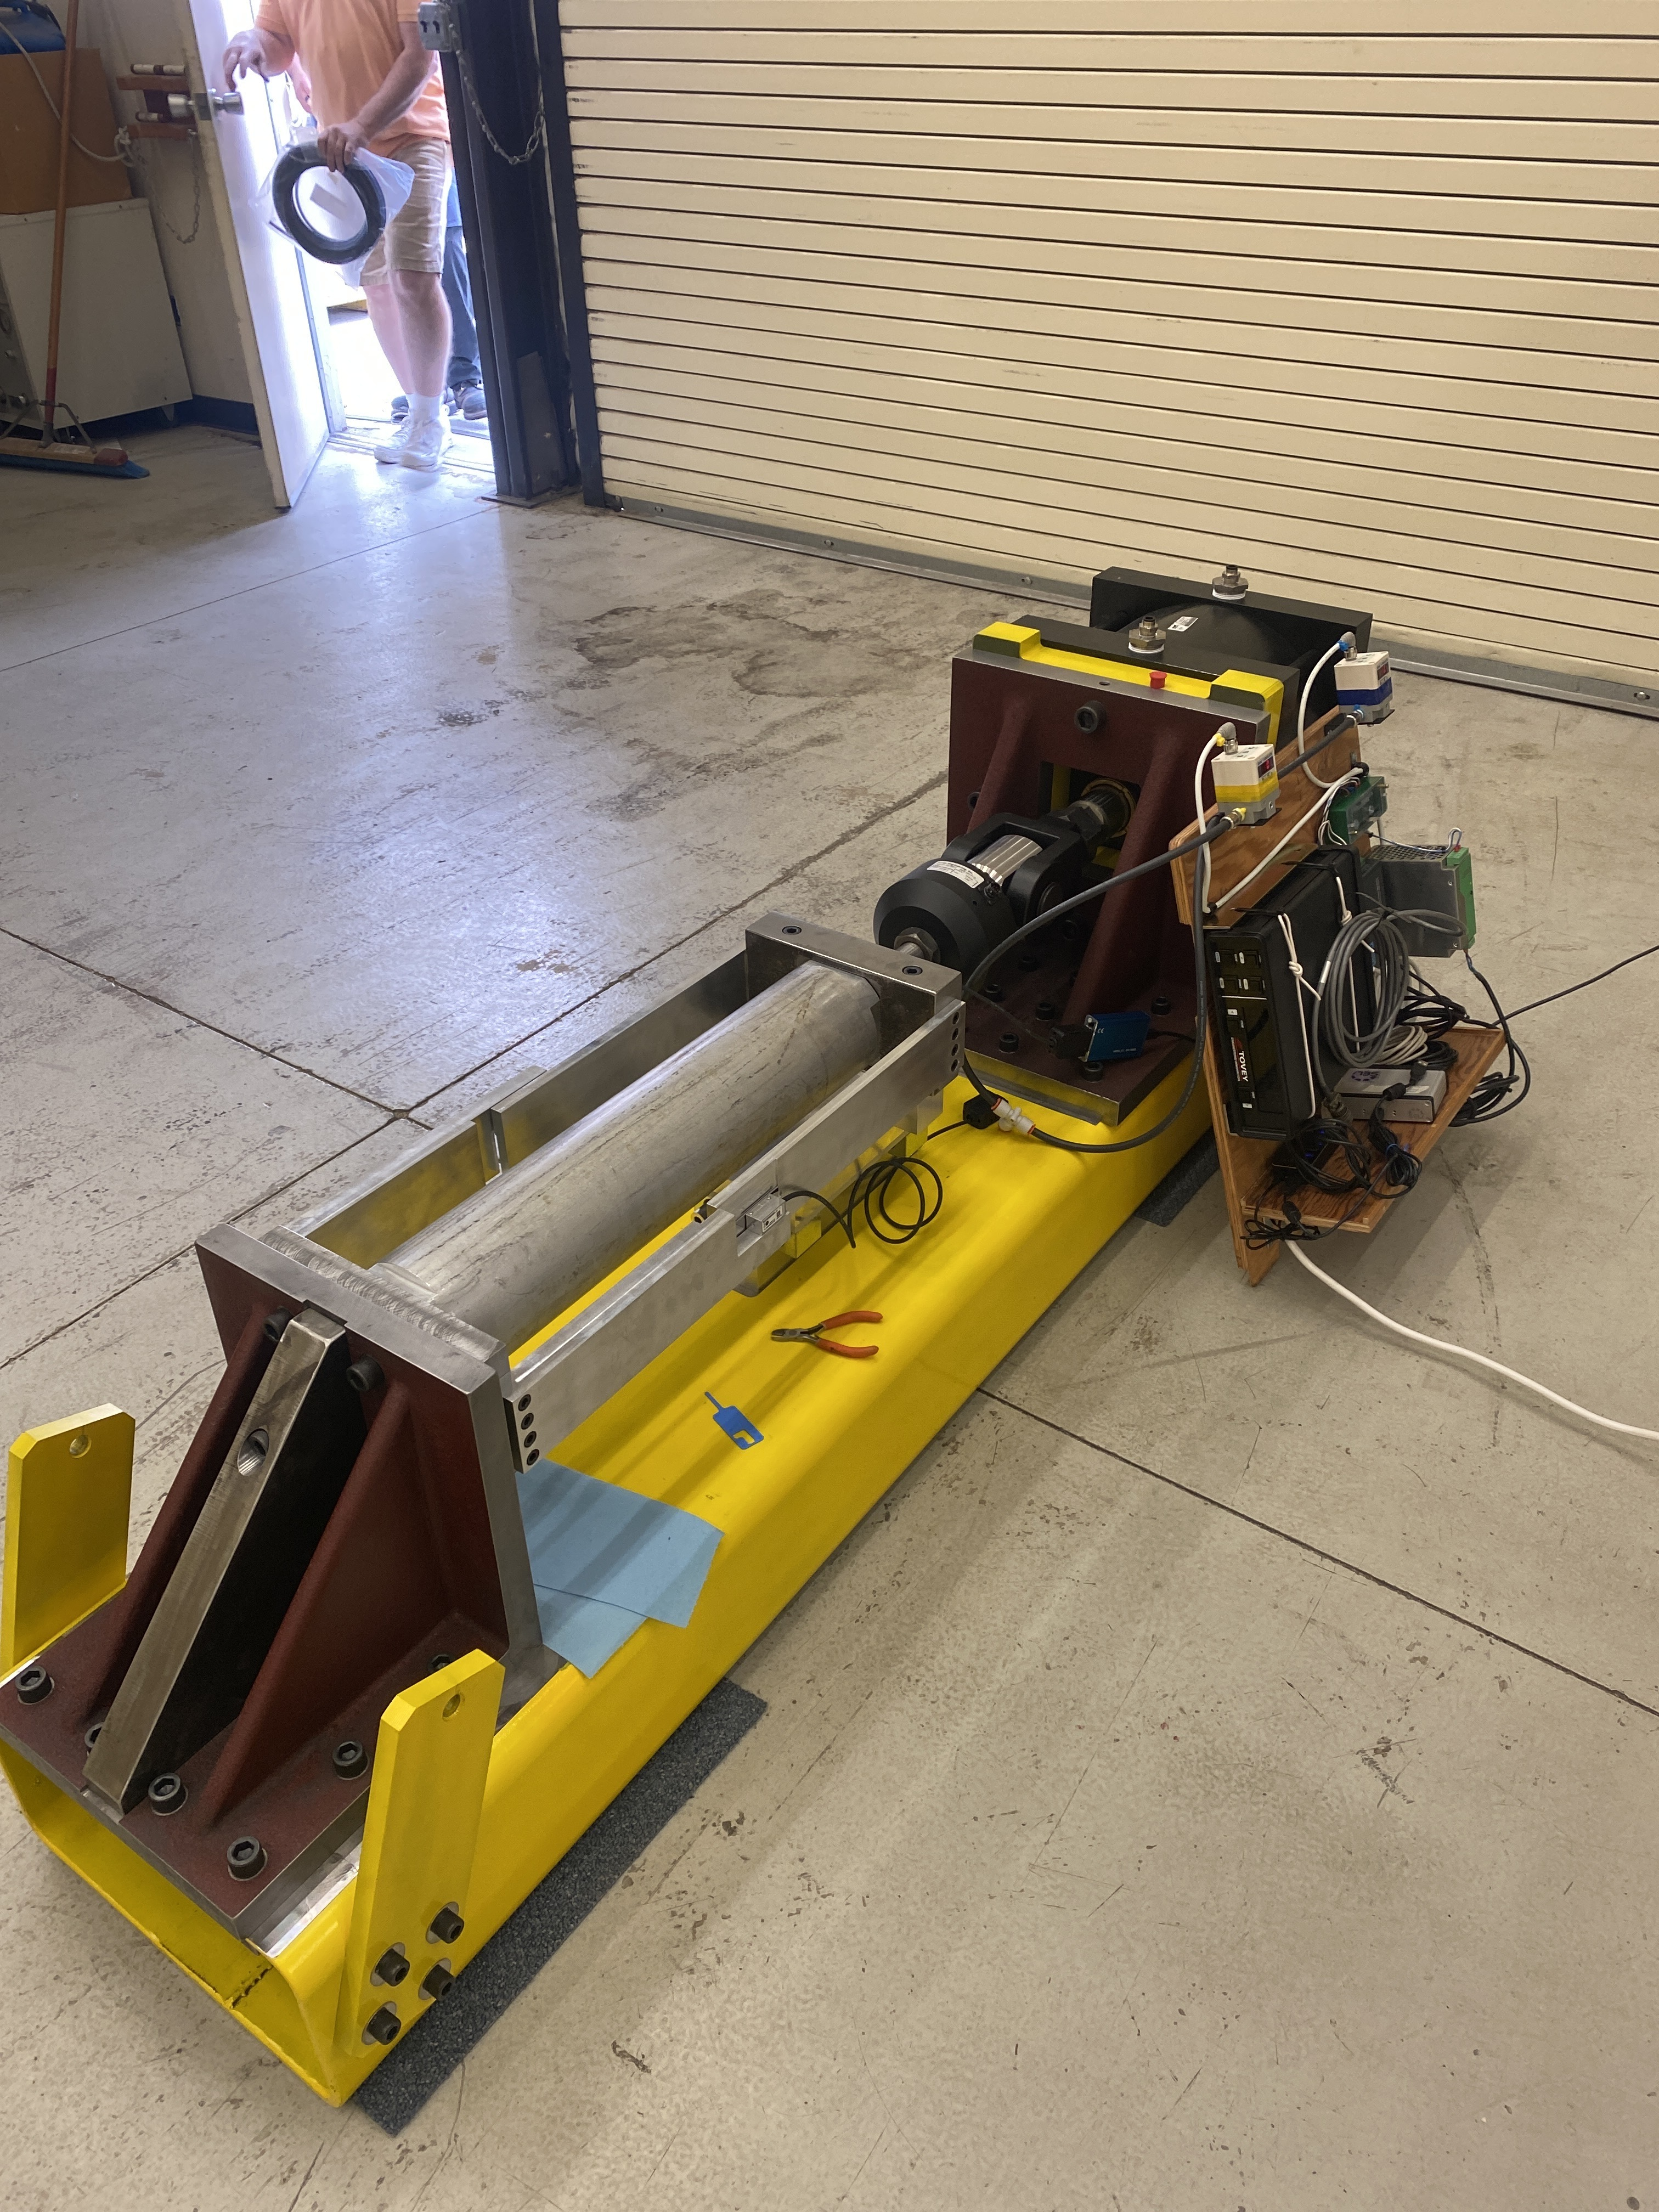
\includegraphics[width=3.12500in]{jira_imgs/3598.jpg}Test Rig with
Actuator:\\
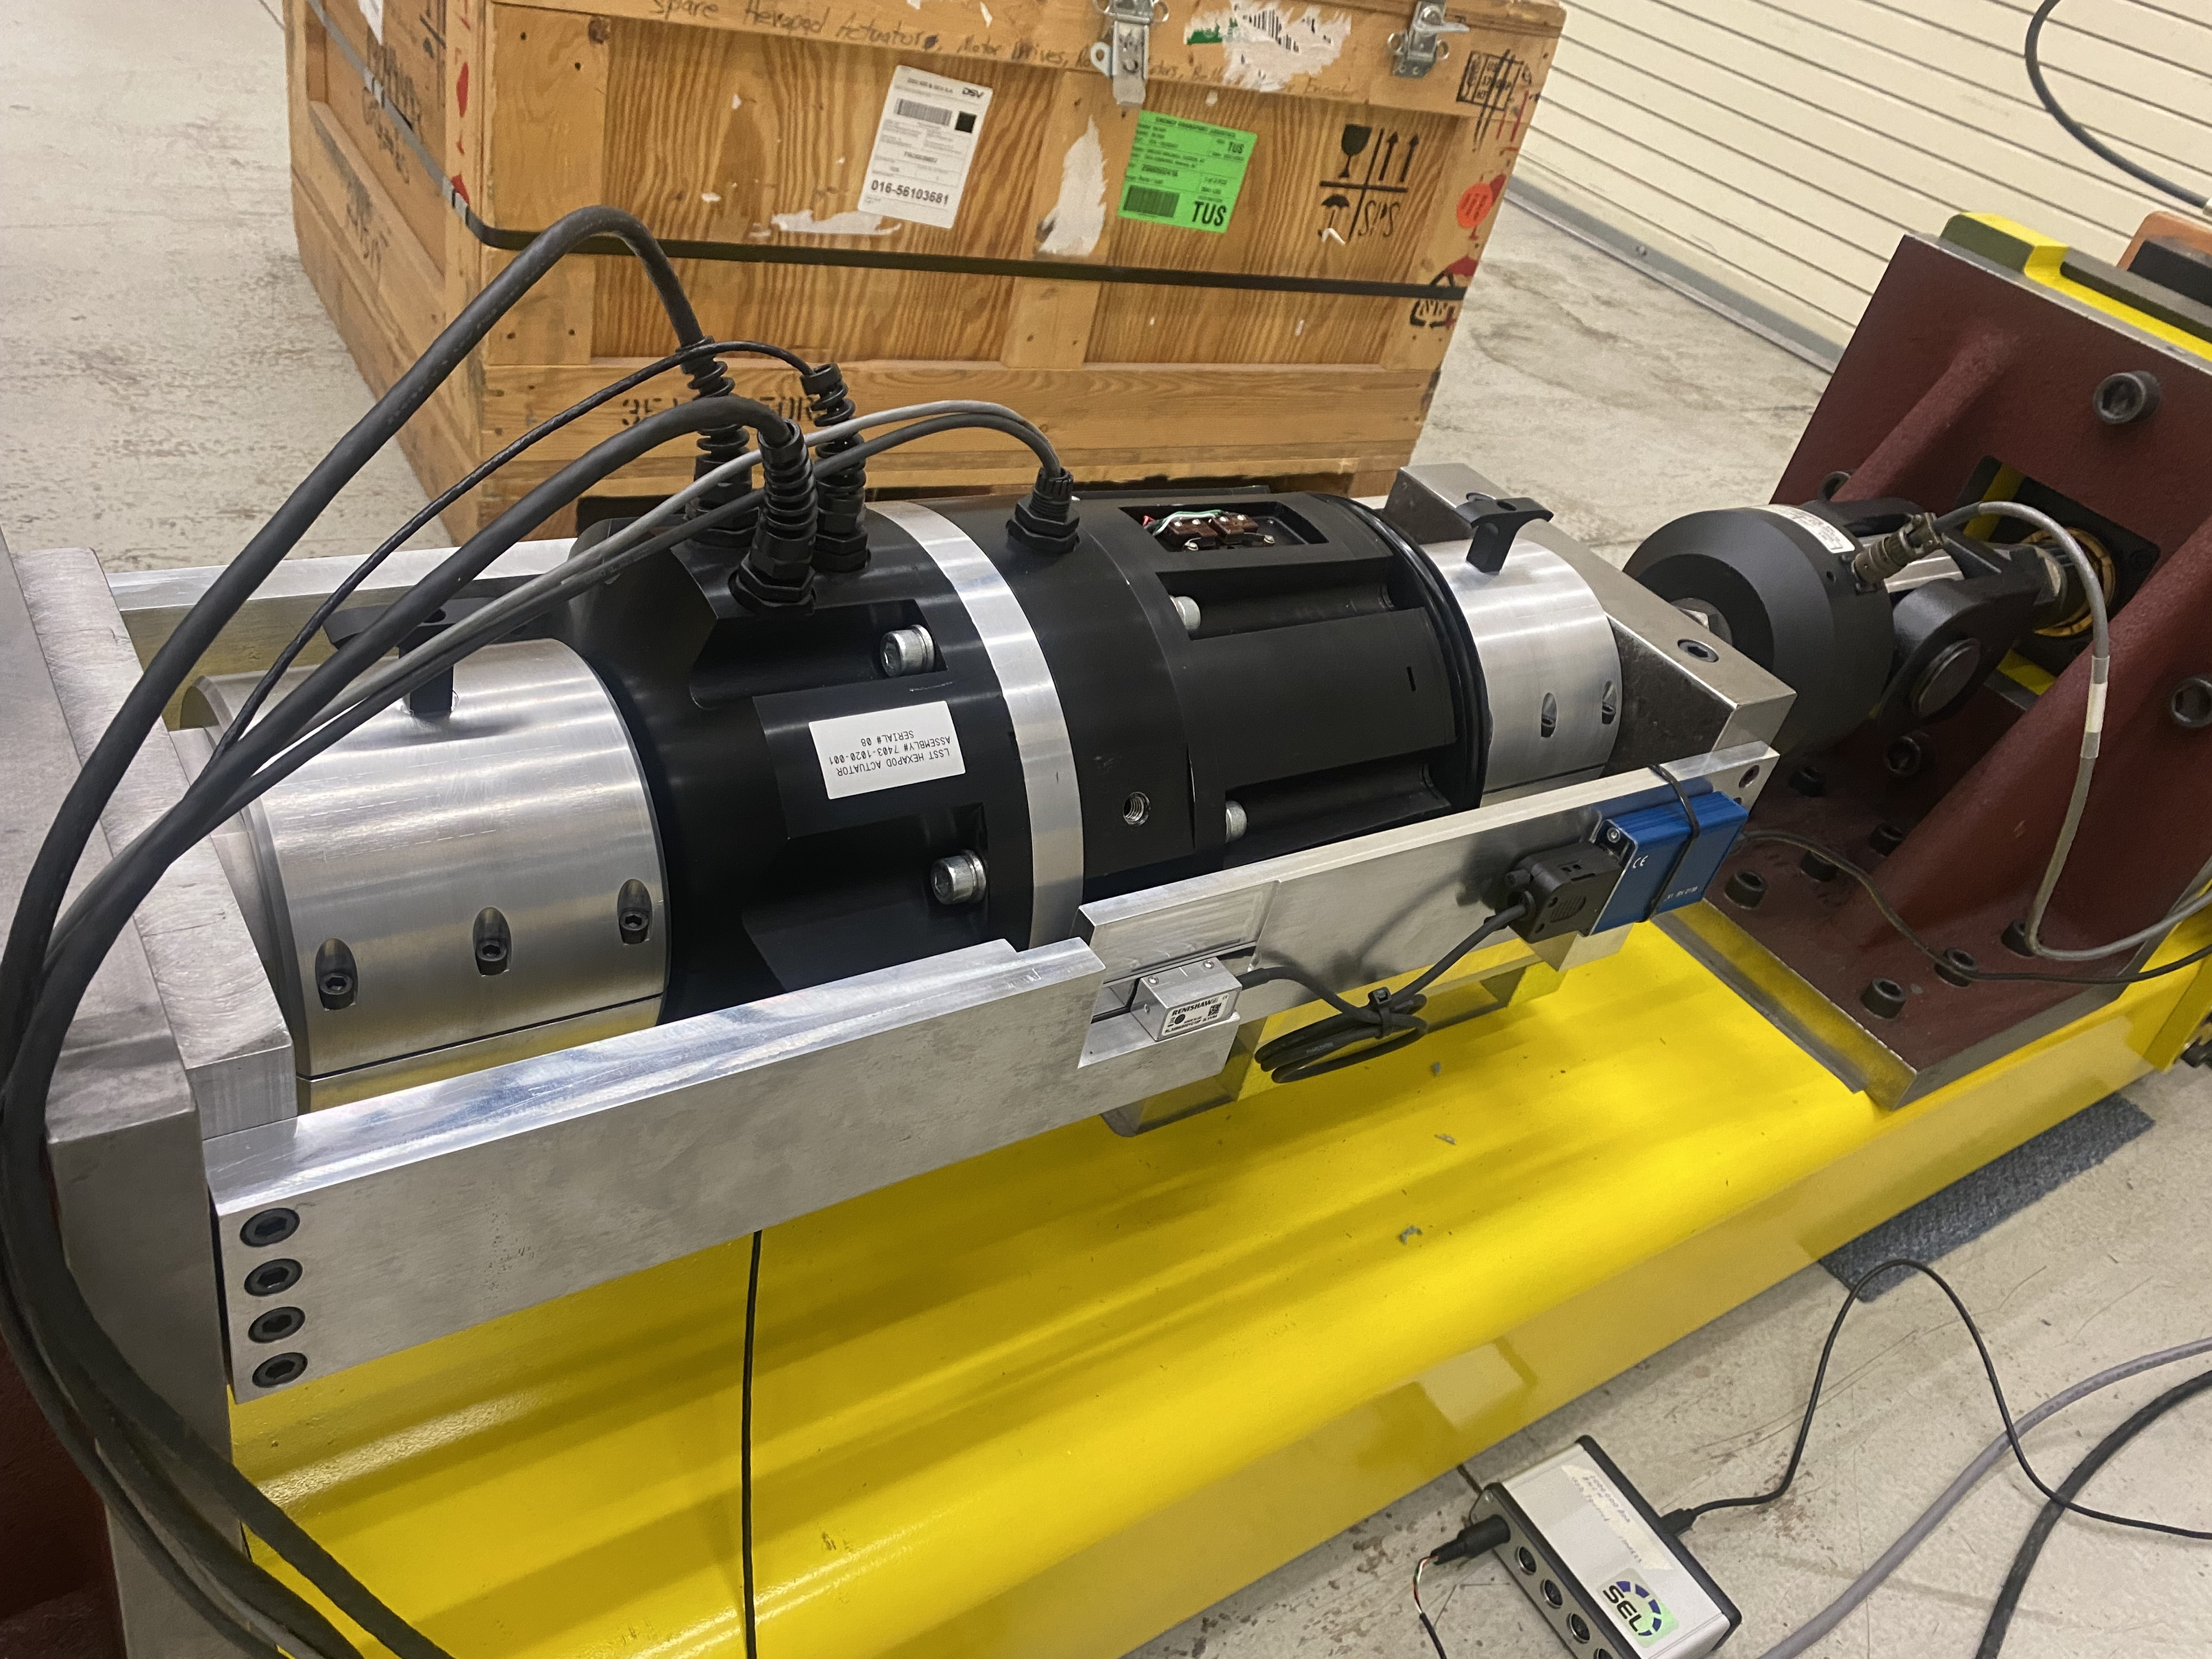
\includegraphics[width=3.12500in]{jira_imgs/3599.jpg}During
Installation, the bolts holding the surrogate/actuator to the interface
block and to the stiff back were torqued to 203 ft-lbs.

}
\begin{tabular}{p{2cm}p{14cm}}
\toprule
Step 3 & Step Execution Status: \textbf{ Pass } \\ \hline
\end{tabular}
 Description \\
{\footnotesize
Verify an air gauge is connected between the air supply and the air
valves.

}
\hdashrule[0.5ex]{\textwidth}{1pt}{3mm}
  Expected Result \\
{\footnotesize
\begin{itemize}
\tightlist
\item
  The air gauge is in position and capable of reading the psi value
  being supplied to the air valves.
\item
  The air gauge should initially show no air being supplied.
\end{itemize}

}
\hdashrule[0.5ex]{\textwidth}{1pt}{3mm}
  Actual Result \\
{\footnotesize
Although the air gauge in the control room was capable of reaching
150psi, for the purposes of these tests, the air supply was never set to
more than 100psi.~

}
\begin{tabular}{p{2cm}p{14cm}}
\toprule
Step 4 & Step Execution Status: \textbf{ Pass } \\ \hline
\end{tabular}
 Description \\
{\footnotesize
Verify the valves for tension and compression are capable of displaying
commanded voltage.~

}
\hdashrule[0.5ex]{\textwidth}{1pt}{3mm}
  Expected Result \\
{\footnotesize
Both air gauges are in place monitoring the output from both the tension
and compression air valves.

}
\hdashrule[0.5ex]{\textwidth}{1pt}{3mm}
  Actual Result \\
{\footnotesize
The valves for tension (blue) and compression (yellow):\\
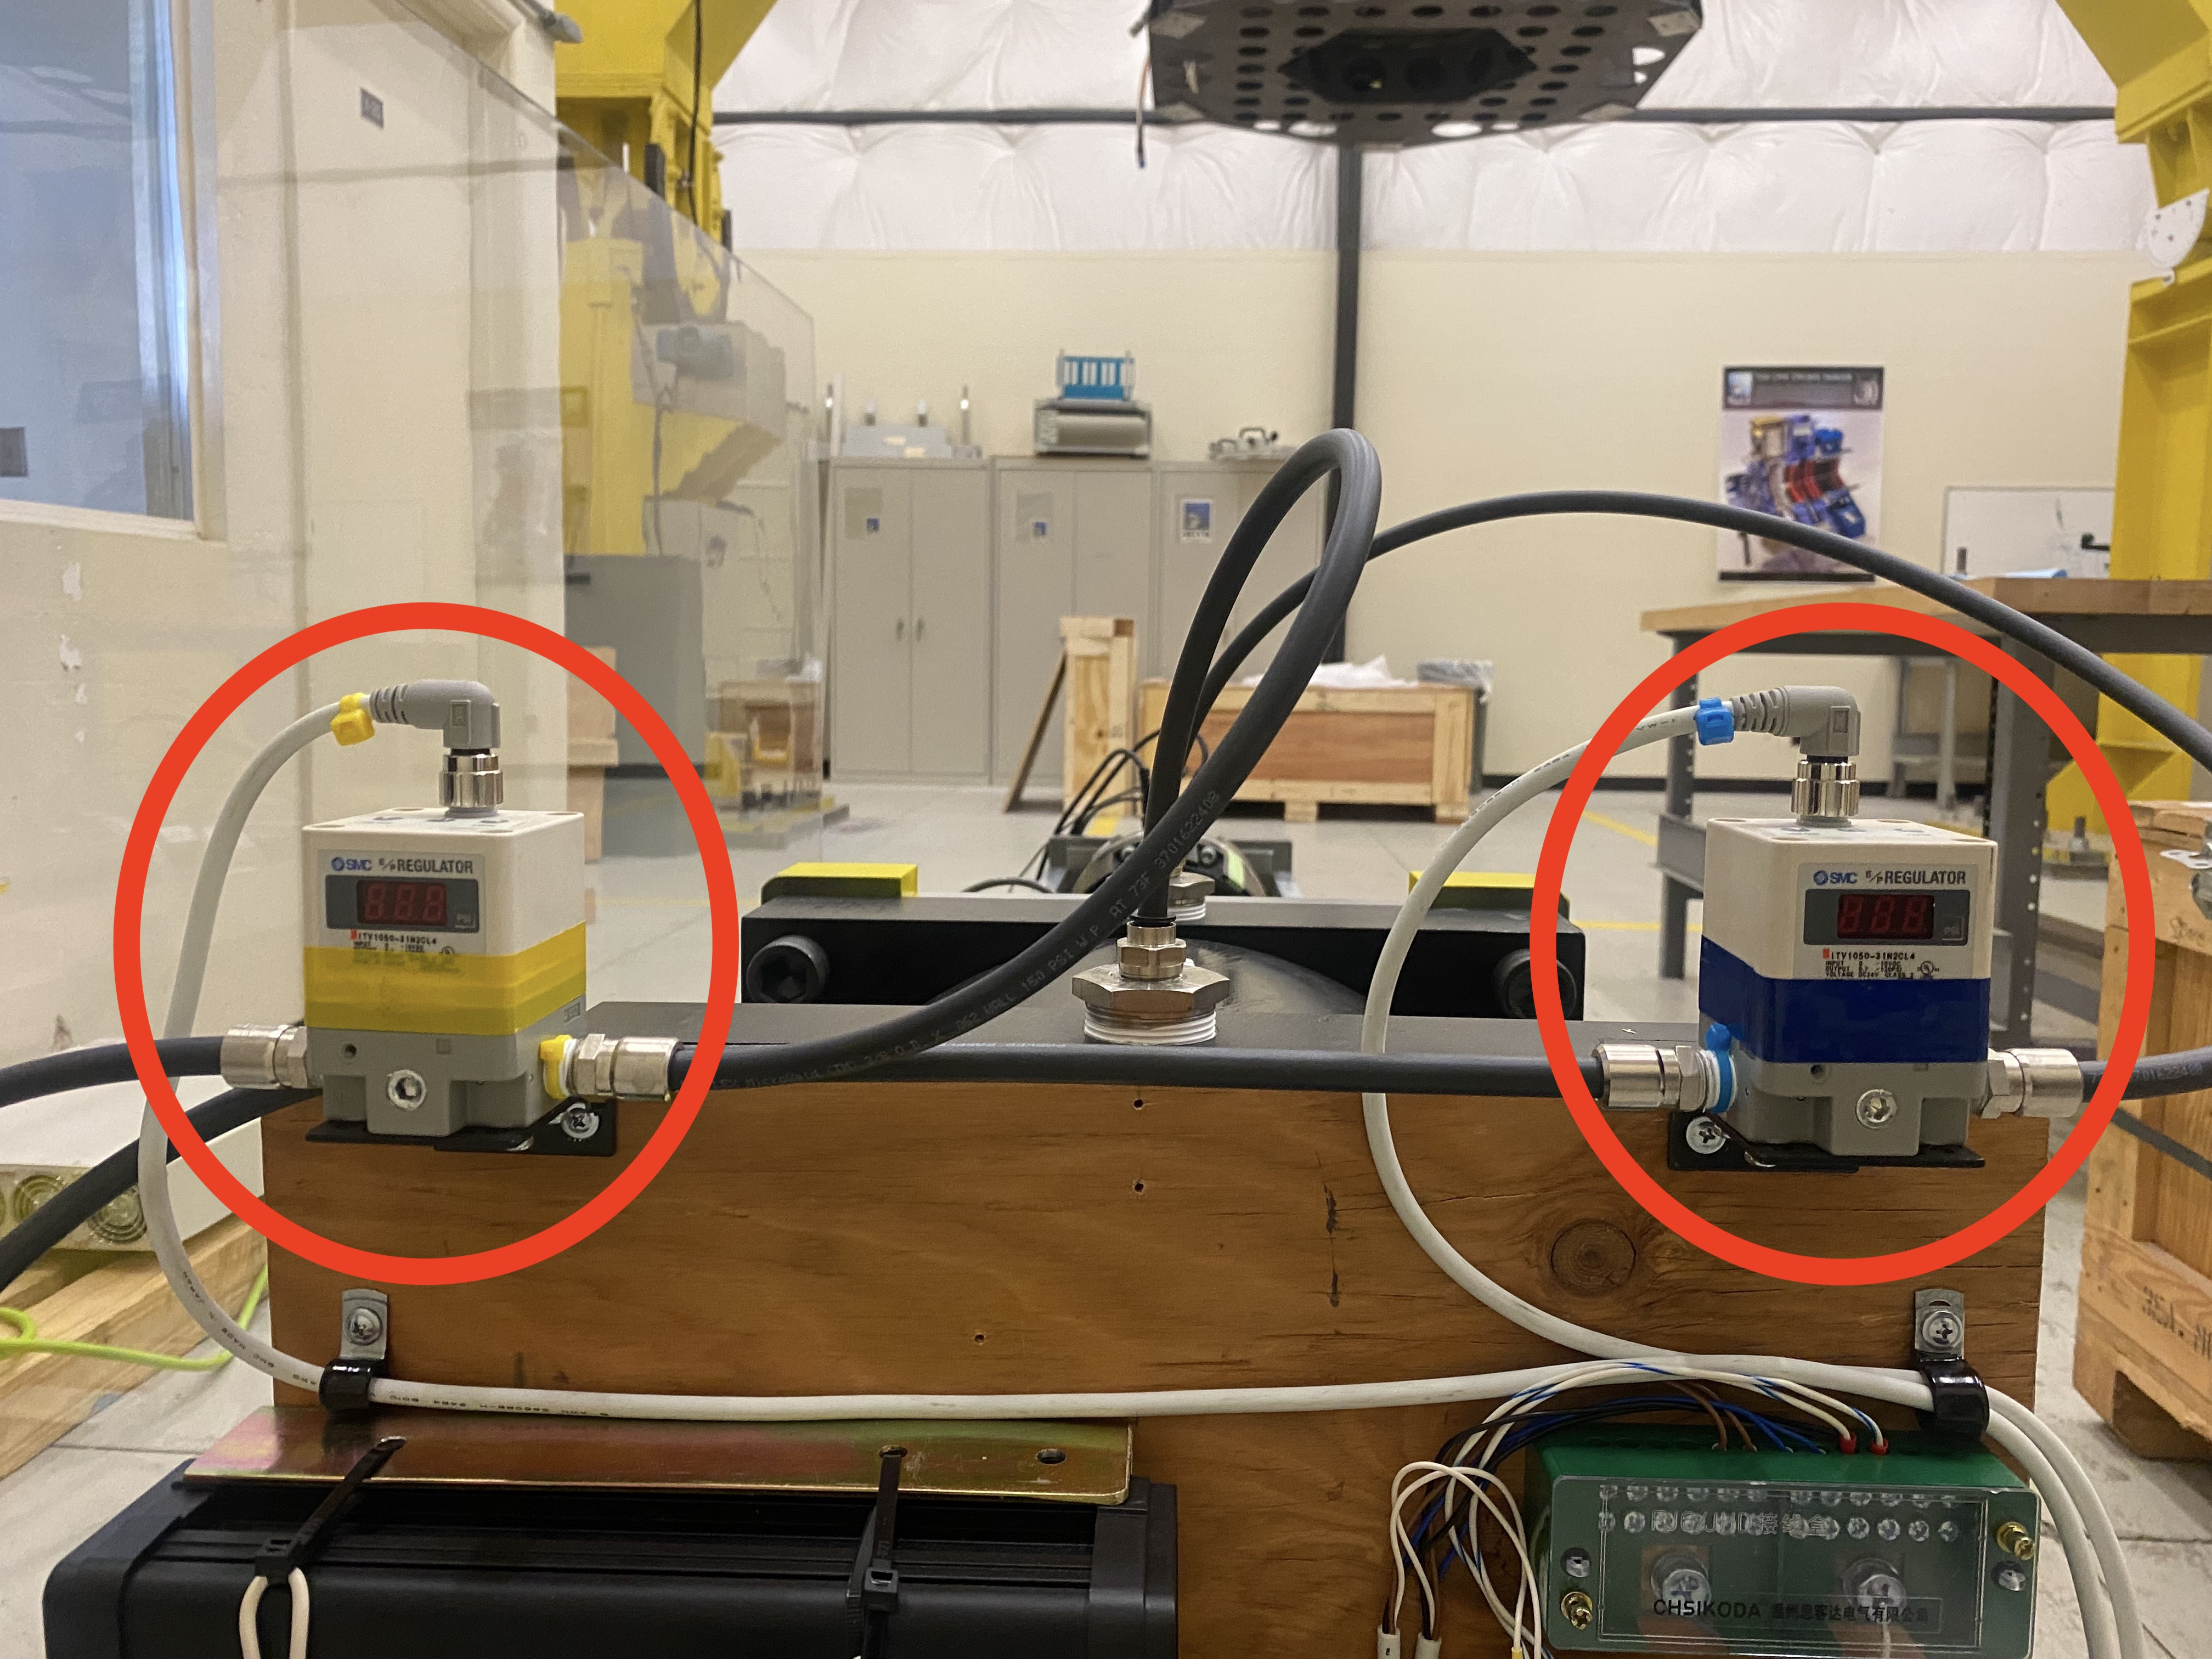
\includegraphics[width=3.12500in]{jira_imgs/3601.jpg}\\
When powered on, the valves displayed the voltage being commanded
through the Labview voltage command function, which correlates to how
much air is being supplied into the pneumatic cylinder. During set up,
the minimum and maximum voltages for each valve was set to 0 and 10V.

}
\begin{tabular}{p{2cm}p{14cm}}
\toprule
Step 5 & Step Execution Status: \textbf{ Pass } \\ \hline
\end{tabular}
 Description \\
{\footnotesize
Make the connection between the two sets of air valves and gauges and
the USB-4716 readout device.\\
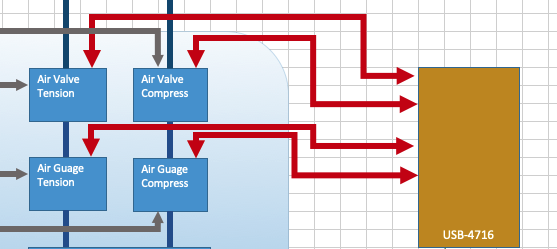
\includegraphics[width=3.12500in]{jira_imgs/3435.png}

}
\hdashrule[0.5ex]{\textwidth}{1pt}{3mm}
  Expected Result \\
{\footnotesize
The air valves and gauges are hooked up to the USB-4716 readout device.~

}
\hdashrule[0.5ex]{\textwidth}{1pt}{3mm}
  Actual Result \\
{\footnotesize
The tension and compression valves were connected to the USB-4716.
However, no additional gauges were placed in series between the valves
and the pneumatic cylinder as it was determined to be redundant and
unnecessary.

}
\begin{tabular}{p{2cm}p{14cm}}
\toprule
Step 6 & Step Execution Status: \textbf{ Pass } \\ \hline
\end{tabular}
 Description \\
{\footnotesize
Make the connection between the MB5U readout electronics and the
renishaw encoders.

}
\hdashrule[0.5ex]{\textwidth}{1pt}{3mm}
  Expected Result \\
{\footnotesize
The MB5U readouts are connected to the encoders.

}
\hdashrule[0.5ex]{\textwidth}{1pt}{3mm}
  Actual Result \\
{\footnotesize
The encoders were connected to the MB5U readout electronics. Both were
mounted onto the arms of the test fixture as seen in the picture
below.\\
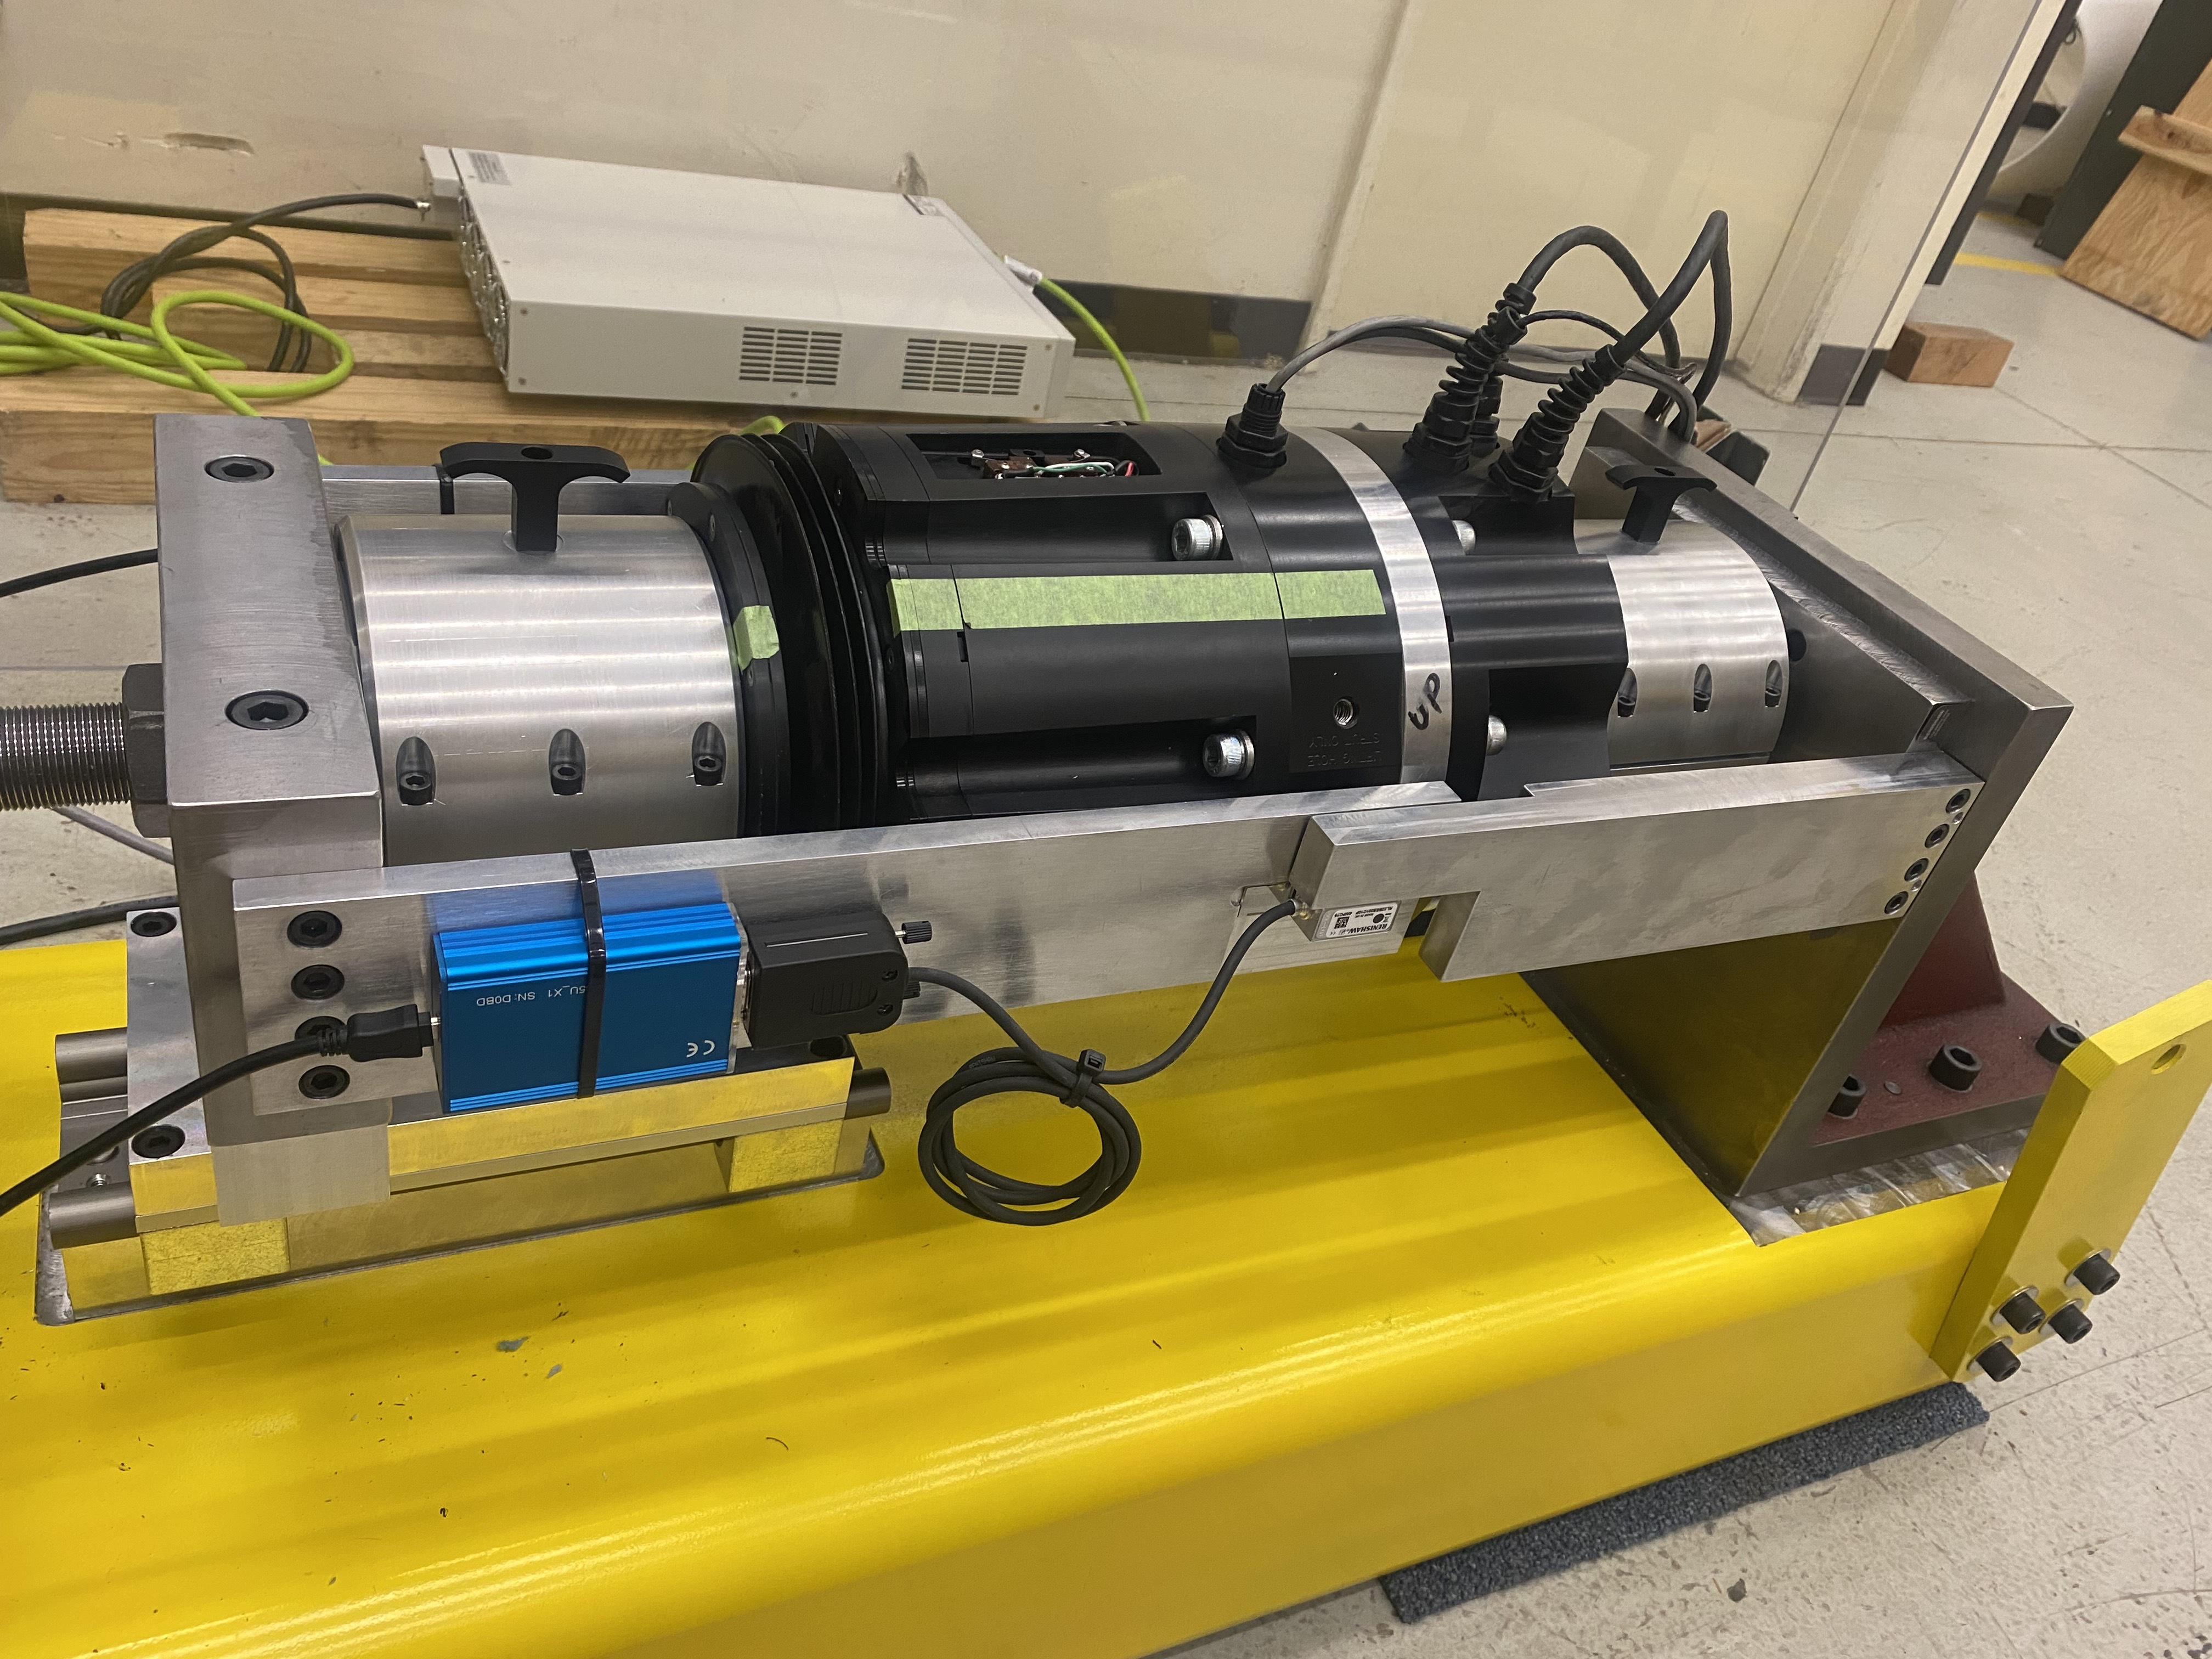
\includegraphics[width=3.12500in]{jira_imgs/3602.jpg}The configuration
that is being shown for this linear encoder and its reader was applied
in the same way to the other side with the other encoder and reader.

}
\begin{tabular}{p{2cm}p{14cm}}
\toprule
Step 7 & Step Execution Status: \textbf{ Pass } \\ \hline
\end{tabular}
 Description \\
{\footnotesize
Make the connection between the 9150 load cell readout electronic and
the load cell.

}
\hdashrule[0.5ex]{\textwidth}{1pt}{3mm}
  Expected Result \\
{\footnotesize
The load cell is connected to the load cell readout electronic.

}
\hdashrule[0.5ex]{\textwidth}{1pt}{3mm}
  Actual Result \\
{\footnotesize
As seen in the picture, the 9150 load cell readout electronic was
included on the mounted board with the rest of the electrical
connections. The load cell readout was directly connected to the load
cell.~\\
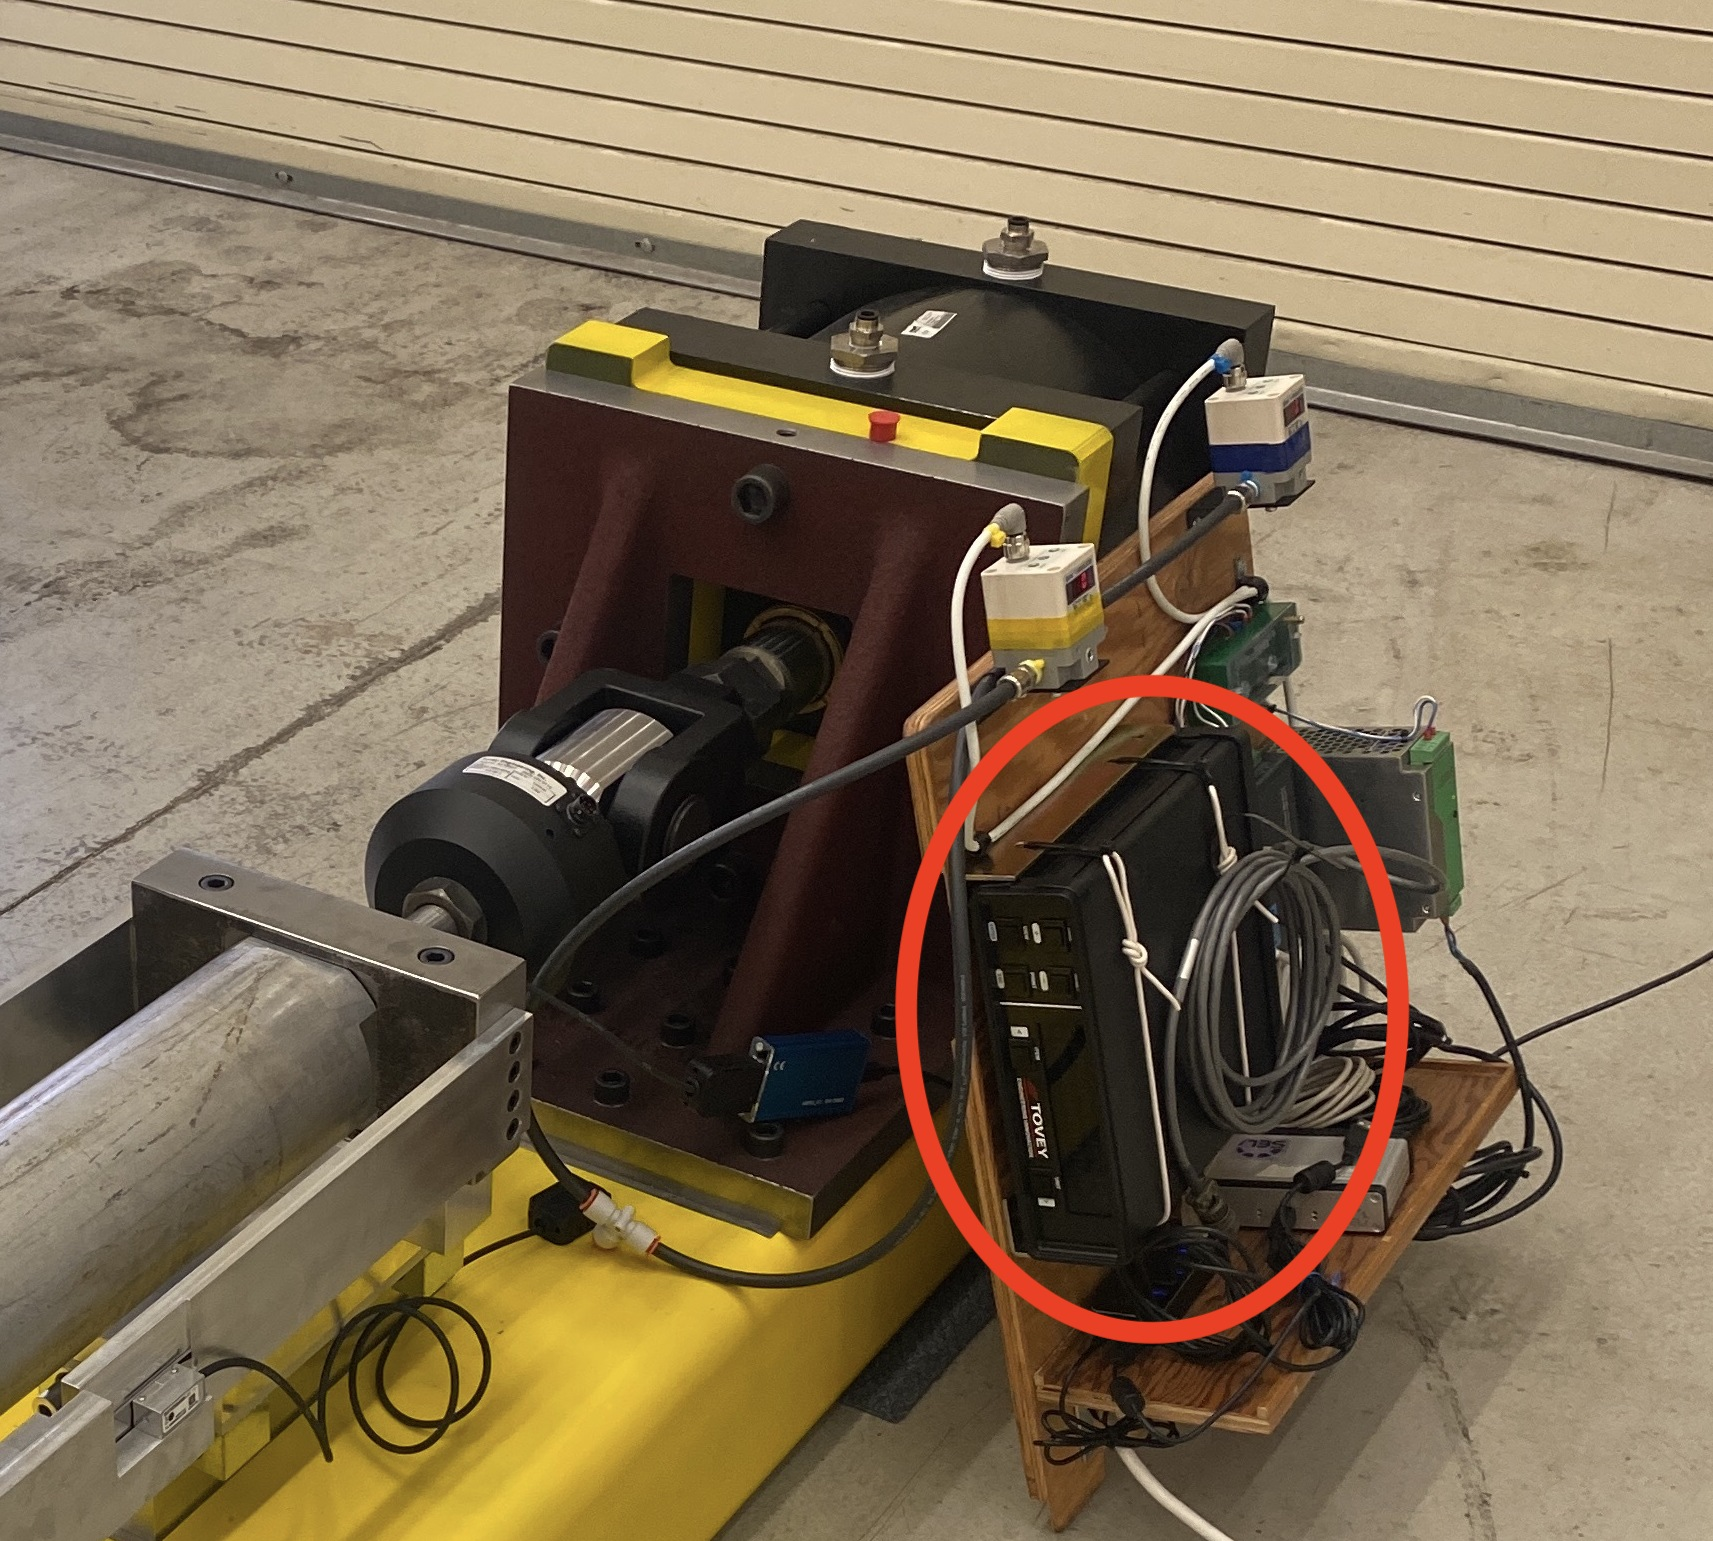
\includegraphics[width=3.12500in]{jira_imgs/3603.jpg}

}
\begin{tabular}{p{2cm}p{14cm}}
\toprule
Step 8 & Step Execution Status: \textbf{ Not Executed } \\ \hline
\end{tabular}
 Description \\
{\footnotesize
Make the connection between the Hexapod Actuator to the thermal
scanner.~

}
\hdashrule[0.5ex]{\textwidth}{1pt}{3mm}
  Expected Result \\
{\footnotesize
The thermal scanner is connected to the hexapod actuator.

}
\hdashrule[0.5ex]{\textwidth}{1pt}{3mm}
  Actual Result \\
{\footnotesize
This was not executed at the time of this test as the internal
temperature scanner cable was not available. However, an external
temperature sensor was able to be connected and readout by the RealTerm
application of the control computer.~

}
\begin{tabular}{p{2cm}p{14cm}}
\toprule
Step 9 & Step Execution Status: \textbf{ Pass } \\ \hline
\end{tabular}
 Description \\
{\footnotesize
Connect the following to the USB 3.0 Hub:

\begin{itemize}
\tightlist
\item
  (2) connections for MB5U Readout Electronic
\item
  USB-4716 Readout Device/Labjack T4
\item
  Temperature Readout
\item
  9150 Load Cell Readout Electronic
\end{itemize}

}
\hdashrule[0.5ex]{\textwidth}{1pt}{3mm}
  Expected Result \\
{\footnotesize
The USB 3.0 Hub is now connected to the readout electronics from the
previous steps.~

}
\hdashrule[0.5ex]{\textwidth}{1pt}{3mm}
  Actual Result \\
{\footnotesize
The USB 3.0 Hub was connected to the 2 MB5U Encoder readers, the
USB-4716 Readout Device for the pneumatic valves and the Tovey 9150 Load
Cell Readout. As mentioned in the previous step, the thermal scanner was
not connected.~

}
\begin{tabular}{p{2cm}p{14cm}}
\toprule
Step 10 & Step Execution Status: \textbf{ Pass } \\ \hline
\end{tabular}
 Description \\
{\footnotesize
Connect the laptop with LabVIEW software to the USB 3.0 Hub.

}
\hdashrule[0.5ex]{\textwidth}{1pt}{3mm}
  Expected Result \\
{\footnotesize
The Laptop is connected to the USB 3.0 Hub and to the subsequent readout
electronics.~

}
\hdashrule[0.5ex]{\textwidth}{1pt}{3mm}
  Actual Result \\
{\footnotesize
A cable was connected from the USB 3.0 Hub by the test rig to the laptop
with LabView in the control room.~

}
\begin{tabular}{p{2cm}p{14cm}}
\toprule
Step 11 & Step Execution Status: \textbf{ Pass } \\ \hline
\end{tabular}
 Description \\
{\footnotesize
Connect the laptop to the Copley Motor drive of the Control Box.

}
\hdashrule[0.5ex]{\textwidth}{1pt}{3mm}
  Expected Result \\
{\footnotesize
The laptop is connected to the control box.

}
\hdashrule[0.5ex]{\textwidth}{1pt}{3mm}
  Actual Result \\
{\footnotesize
The Control Box was set up next to the test rig and connected to the
same USB 3.0 Hub already connected to the laptop.~

}
\begin{tabular}{p{2cm}p{14cm}}
\toprule
Step 12 & Step Execution Status: \textbf{ Pass } \\ \hline
\end{tabular}
 Description \\
{\footnotesize
Set up the USB 3.0 Hub close to the test fixture and connect it to a
power source.~

}
\hdashrule[0.5ex]{\textwidth}{1pt}{3mm}
  Expected Result \\
{\footnotesize
The USB 3.0 Hub is connected and all readout devices are powered on.~

}
\hdashrule[0.5ex]{\textwidth}{1pt}{3mm}
  Actual Result \\
{\footnotesize
A power strip was attached to the electronics board and powered the USB
3.0 Hub.\\
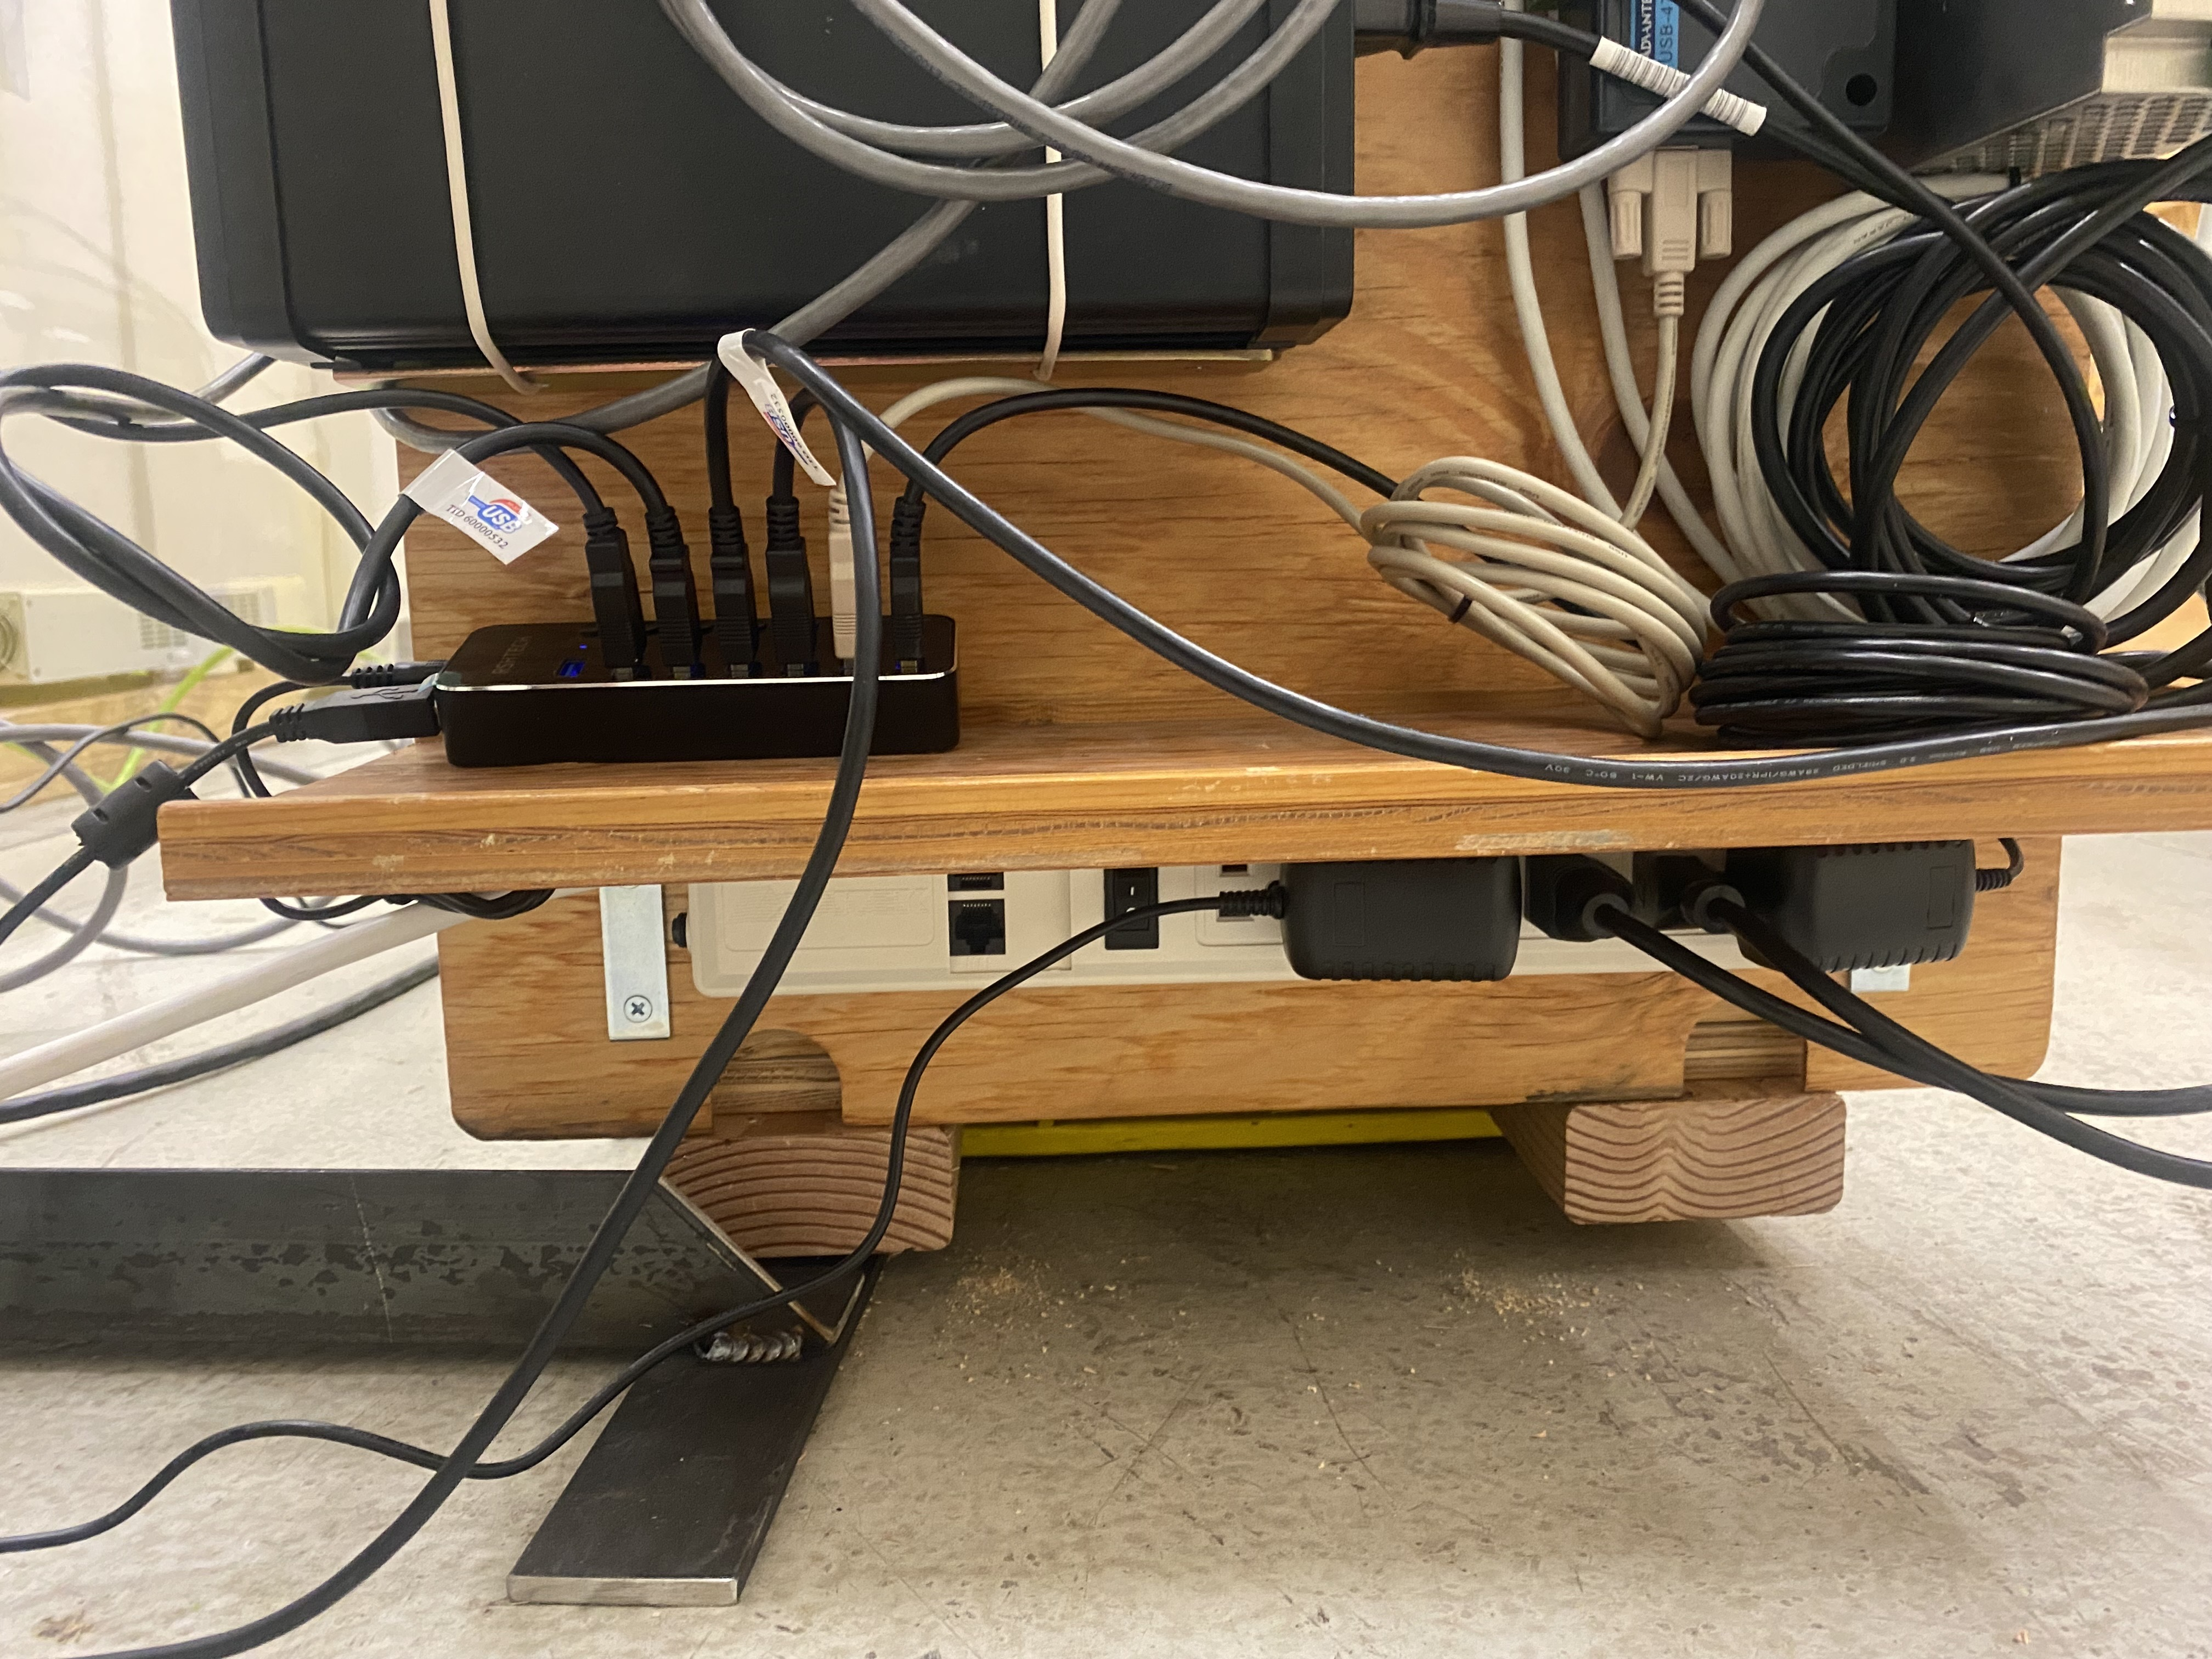
\includegraphics[width=3.12500in]{jira_imgs/3604.jpg}

}
\begin{tabular}{p{2cm}p{14cm}}
\toprule
Step 13 & Step Execution Status: \textbf{ Pass } \\ \hline
\end{tabular}
 Description \\
{\footnotesize
Verify that the output data from the readout devices are available on
the laptop.

}
\hdashrule[0.5ex]{\textwidth}{1pt}{3mm}
  Expected Result \\
{\footnotesize
The laptop is seen to be able to communicate with the readout devices.

}
\hdashrule[0.5ex]{\textwidth}{1pt}{3mm}
  Actual Result \\
{\footnotesize
Using LabView, we were able to confirm that we were able to read the
data from the encoder read heads.~

}
\begin{tabular}{p{2cm}p{14cm}}
\toprule
Step 14 & Step Execution Status: \textbf{ Pass } \\ \hline
\end{tabular}
 Description \\
{\footnotesize
Open Labview 2021 in the computer used for Test Setup.

}
\hdashrule[0.5ex]{\textwidth}{1pt}{3mm}
  Expected Result \\
{\footnotesize
Labview 2021 opens successfully.

}
\hdashrule[0.5ex]{\textwidth}{1pt}{3mm}
  Actual Result \\
{\footnotesize
LabView was available on the test computer.~

}
\begin{tabular}{p{2cm}p{14cm}}
\toprule
Step 15 & Step Execution Status: \textbf{ Pass } \\ \hline
\end{tabular}
 Description \\
{\footnotesize
Open the Labview VI files from the project directory including sub VIs-
Tovey Closed loop.vi, Voltage Regulation.vi and Biss Reader.vi

}
\hdashrule[0.5ex]{\textwidth}{1pt}{3mm}
  Expected Result \\
{\footnotesize
Front panel of VI and sub VI files open without any error.

}
\hdashrule[0.5ex]{\textwidth}{1pt}{3mm}
  Actual Result \\
{\footnotesize
The LabView VI files that we used were updated and renamed. The new
files can be found attached to this test step.

}
\begin{tabular}{p{2cm}p{14cm}}
\toprule
Step 16 & Step Execution Status: \textbf{ Pass } \\ \hline
\end{tabular}
 Description \\
{\footnotesize
Configure the Biss Reader.vi file with the appropriate configuration
file and following the IBISS operation manual.~

}
\hdashrule[0.5ex]{\textwidth}{1pt}{3mm}
  Expected Result \\
{\footnotesize
\href{https://jira.lsstcorp.org/rest/tests/1.0/attachment/3555}{BiSS\_config.cfg}
is loaded in the LabView configuration (Misc Tab under Load DLL). The
configuration file is based on the IBISS operation manual.

}
\hdashrule[0.5ex]{\textwidth}{1pt}{3mm}
  Actual Result \\
{\footnotesize
As stated in the previous step, the BISS Reader file has been modified.
As a result, the instructions for loading the DLL config file are more
straightforward. T

}
\begin{tabular}{p{2cm}p{14cm}}
\toprule
Step 17 & Step Execution Status: \textbf{ Pass } \\ \hline
\end{tabular}
 Description \\
{\footnotesize
Click Run button on the on the block diagram toolbar of the Labview VI
front panel.

}
\hdashrule[0.5ex]{\textwidth}{1pt}{3mm}
  Expected Result \\
{\footnotesize
LabView VI and ~associated sub Vi runs successfully. Initially all the
graphs and input values will be blank.

}
\hdashrule[0.5ex]{\textwidth}{1pt}{3mm}
  Actual Result \\
{\footnotesize
The LabView VI were able to be run without errors.~

}
\begin{tabular}{p{2cm}p{14cm}}
\toprule
Step 18 & Step Execution Status: \textbf{ Pass } \\ \hline
\end{tabular}
 Description \\
{\footnotesize
Send a command through LabVIEW ~voltage Regulation.vi to set the voltage
on the compression valve only to 3V.

}
\hdashrule[0.5ex]{\textwidth}{1pt}{3mm}
  Expected Result \\
{\footnotesize
The command is accepted, the pneumatic valve shows the applied voltage
only on the compression valve and the applied compression force can be
seen on the LabView front panel Time vs Load graph.~

}
\hdashrule[0.5ex]{\textwidth}{1pt}{3mm}
  Actual Result \\
{\footnotesize
During the Hexapod Initial Validation test
(\href{https://jira.lsstcorp.org/secure/Tests.jspa\#/testPlayer/testExecution/LVV-E2728}{LVV-E2728}),
we verified that we were able to apply voltages for both the tension and
compression valves through Labview and their corresponding values in
force being applied.~

}
\begin{tabular}{p{2cm}p{14cm}}
\toprule
Step 19 & Step Execution Status: \textbf{ Pass } \\ \hline
\end{tabular}
 Description \\
{\footnotesize
Send a command through LabVIEW voltage Regulation.vi to reset the
compression valve to 0V.

}
\hdashrule[0.5ex]{\textwidth}{1pt}{3mm}
  Expected Result \\
{\footnotesize
The command is accepted. The applied force can be seen as zero load on
the LabView front panel Time vs Load graph. Load Cell Reader also shows
zero load.

}
\hdashrule[0.5ex]{\textwidth}{1pt}{3mm}
  Actual Result \\
{\footnotesize
During the Hexapod Initial Validation test
(\href{https://jira.lsstcorp.org/secure/Tests.jspa\#/testPlayer/testExecution/LVV-E2728}{LVV-E2728}),
we verified that we were able to apply voltages for both the tension and
compression valves through Labview and their corresponding values in
force being applied.

}
\begin{tabular}{p{2cm}p{14cm}}
\toprule
Step 20 & Step Execution Status: \textbf{ Pass } \\ \hline
\end{tabular}
 Description \\
{\footnotesize
Send a command through LabVIEW to reset the tension valve to 3V.

}
\hdashrule[0.5ex]{\textwidth}{1pt}{3mm}
  Expected Result \\
{\footnotesize
The command is accepted, the readout electronic shows the applied
voltage only on the tension valve and the applied tension force can be
seen on the LabView front panel Time vs Load graph.

}
\hdashrule[0.5ex]{\textwidth}{1pt}{3mm}
  Actual Result \\
{\footnotesize
During the Hexapod Initial Validation test
(\href{https://jira.lsstcorp.org/secure/Tests.jspa\#/testPlayer/testExecution/LVV-E2728}{LVV-E2728}),
we verified that we were able to apply voltages for both the tension and
compression valves through Labview and their corresponding values in
force being applied.

}
\begin{tabular}{p{2cm}p{14cm}}
\toprule
Step 21 & Step Execution Status: \textbf{ Pass } \\ \hline
\end{tabular}
 Description \\
{\footnotesize
Send a command through LabVIEW to reset the tension valve to 0V.

}
\hdashrule[0.5ex]{\textwidth}{1pt}{3mm}
  Expected Result \\
{\footnotesize
The command is accepted, the readout electronic no longer shows the
applied voltage on the tension valve and there is no longer any tension
force on the LabView front panel Time vs Load graph.

}
\hdashrule[0.5ex]{\textwidth}{1pt}{3mm}
  Actual Result \\
{\footnotesize
During the Hexapod Initial Validation test
(\href{https://jira.lsstcorp.org/secure/Tests.jspa\#/testPlayer/testExecution/LVV-E2728}{LVV-E2728}),
we verified that we were able to apply voltages for both the tension and
compression valves through Labview and their corresponding values in
force being applied.

}
\begin{tabular}{p{2cm}p{14cm}}
\toprule
Step 22 & Step Execution Status: \textbf{ Pass } \\ \hline
\end{tabular}
 Description \\
{\footnotesize
Verify the laptop is reading the renishaw scales usinthe Biss Reader.vi
file and determine the zero stroke position.

}
\hdashrule[0.5ex]{\textwidth}{1pt}{3mm}
  Test Data \\
 {\footnotesize
\textbf{Note:~}Moog's original test procedure cited the zero position to
be at 40mm since the full length was 80mm.

}
\hdashrule[0.5ex]{\textwidth}{1pt}{3mm}
  Expected Result \\
{\footnotesize
40mm encoder readings shown in Labview front panel of the .vi file.~\\
The zero stroke position has been determined and can be used as a
reference for the offset of future moves.

}
\hdashrule[0.5ex]{\textwidth}{1pt}{3mm}
  Actual Result \\
{\footnotesize
Using the modified Encoder A (D13B) and Load Cell.vi and Encoder B
(D0BD).vi, we verified the position of the readings of each of the
external encoders. Then using the copley control software, we verified
the position of the external encoders when the actuator was in the
center stroke position. As documented in the next steps, we saw both
encoders reading about 39.5mm

}
\begin{tabular}{p{2cm}p{14cm}}
\toprule
Step 23 & Step Execution Status: \textbf{ Pass } \\ \hline
\end{tabular}
 Description \\
{\footnotesize
Using the Copley Software, drive the actuator to the positive limit
switch and take note of the values measured by the Copley Software and
the Encoder Readings.

}
\hdashrule[0.5ex]{\textwidth}{1pt}{3mm}
  Expected Result \\
{\footnotesize
The actuator is able to hit the positive limit switch and the values are
recorded.

}
\hdashrule[0.5ex]{\textwidth}{1pt}{3mm}
  Actual Result \\
{\footnotesize
The positive limit switch was reached reading the following values:

\begin{itemize}
\tightlist
\item
  Copley Software: Active Load Position = -25.904mm
\item
  Encoder A (D13B) = 25.390mm
\item
  Encoder B (D0BD) = 25.068mm
\end{itemize}

Note: No load was applied during this step

}
\begin{tabular}{p{2cm}p{14cm}}
\toprule
Step 24 & Step Execution Status: \textbf{ Pass } \\ \hline
\end{tabular}
 Description \\
{\footnotesize
Using the Copley Software, drive the actuator to the negative limit
switch and take note of the values measured by the Copley Software and
the Encoder Readings.

}
\hdashrule[0.5ex]{\textwidth}{1pt}{3mm}
  Expected Result \\
{\footnotesize
The actuator is able to hit the negative limit switch and the values are
recorded.

}
\hdashrule[0.5ex]{\textwidth}{1pt}{3mm}
  Actual Result \\
{\footnotesize
The negative limit switch was reached reading the following values:

\begin{itemize}
\tightlist
\item
  Copley Software: Active Load Position = -54.501mm
\item
  Encoder A (D13B) = 53.982mm
\item
  Encoder B (D0BD) = 53.645mm
\end{itemize}

Note: No load was applied during this step\\[2\baselineskip]The overall
travel = 28.597mm\\
The zero position should be set to exactly half the overall travel from
each limit switch (14.298mm)\\
Therefore, the zero position as reported by the Copley =
\textbf{-40.202mm or -40202000 counts}

}

\paragraph{ LVV-T2427 - Hexapod - Actuator Back Driving Test }\mbox{}\\

Version \textbf{1}.
Status \textbf{Approved}.
Open  \href{https://jira.lsstcorp.org/secure/Tests.jspa#/testCase/LVV-T2427}{\textit{ LVV-T2427 } }
test case in Jira.

The objective of this test case is to verify that removing the power
from an actuator will not cause the actuator to back drive even with the
application of different loads.

\textbf{ Preconditions}:\\
Proofing 200\% load test should be performed before running the
back-driving test.~

Execution status: {\bf In Progress }

Final comment:\\The proofing 200\% load test will not be conducted as part of this test
cycle. Therefore, it was not a pre-requisite to executing this test
case. However, we did validate the test rig was capable of applying
200\% load (+/-60kN) with the surrogate. See
\href{https://jira.lsstcorp.org/secure/Tests.jspa\#/testPlayer/testExecution/LVV-E2728}{LVV-E2728}.


Detailed steps results:

\begin{tabular}{p{2cm}p{14cm}}
\toprule
Step 1 & Step Execution Status: \textbf{ Pass } \\ \hline
\end{tabular}
 Description \\
{\footnotesize
Open Labview 2021 in the computer used for Test Setup.

}
\hdashrule[0.5ex]{\textwidth}{1pt}{3mm}
  Test Data \\
 {\footnotesize
\textbf{Note:~}The first three steps are conditional because these steps
are included as part of the Test Setup procedure and may not be
necessary if LabView is still open.

}
\hdashrule[0.5ex]{\textwidth}{1pt}{3mm}
  Expected Result \\
{\footnotesize
Labview 2021 opens successfully.

}
\hdashrule[0.5ex]{\textwidth}{1pt}{3mm}
  Actual Result \\
{\footnotesize
Labview has been opened.~

}
\begin{tabular}{p{2cm}p{14cm}}
\toprule
Step 2 & Step Execution Status: \textbf{ Pass } \\ \hline
\end{tabular}
 Description \\
{\footnotesize
Open Labview 2021 in the computer used for Test Setup.

}
\hdashrule[0.5ex]{\textwidth}{1pt}{3mm}
  Test Data \\
 {\footnotesize
\textbf{Note:~}The first three steps are conditional because these steps
are included as part of the Test Setup procedure and may not be
necessary if LabView is still open.

}
\hdashrule[0.5ex]{\textwidth}{1pt}{3mm}
  Expected Result \\
{\footnotesize
Labview 2021 opens successfully.

}
\hdashrule[0.5ex]{\textwidth}{1pt}{3mm}
  Actual Result \\
{\footnotesize
Labview was already open from the first test iteration.

}
\begin{tabular}{p{2cm}p{14cm}}
\toprule
Step 3 & Step Execution Status: \textbf{ Pass } \\ \hline
\end{tabular}
 Description \\
{\footnotesize
Run the following VI's:

\begin{itemize}
\tightlist
\item
  Encoder A (D13B) and Load Cell.vi
\item
  Encoder B (D0BD).vi
\end{itemize}

}
\hdashrule[0.5ex]{\textwidth}{1pt}{3mm}
  Test Data \\
 {\footnotesize
\textbf{Note:~}Each vi is responsible for reading one encoder.

}
\hdashrule[0.5ex]{\textwidth}{1pt}{3mm}
  Expected Result \\
{\footnotesize
Front panel of VI's open without any error.

}
\hdashrule[0.5ex]{\textwidth}{1pt}{3mm}
  Actual Result \\
{\footnotesize
The VI's were opened with no issue.

}
\begin{tabular}{p{2cm}p{14cm}}
\toprule
Step 4 & Step Execution Status: \textbf{ Pass } \\ \hline
\end{tabular}
 Description \\
{\footnotesize
Run the following VI's:

\begin{itemize}
\tightlist
\item
  Encoder A (D13B) and Load Cell.vi
\item
  Encoder B (D0BD).vi
\end{itemize}

}
\hdashrule[0.5ex]{\textwidth}{1pt}{3mm}
  Test Data \\
 {\footnotesize
\textbf{Note:~}Each vi is responsible for reading one encoder.

}
\hdashrule[0.5ex]{\textwidth}{1pt}{3mm}
  Expected Result \\
{\footnotesize
Front panel of VI's open without any error.

}
\hdashrule[0.5ex]{\textwidth}{1pt}{3mm}
  Actual Result \\
{\footnotesize
Labview VI's were already open from the first test iteration.

}
\begin{tabular}{p{2cm}p{14cm}}
\toprule
Step 5 & Step Execution Status: \textbf{ Pass } \\ \hline
\end{tabular}
 Description \\
{\footnotesize
Click Run button on the block diagram toolbar of the Labview VI front
panel.

}
\hdashrule[0.5ex]{\textwidth}{1pt}{3mm}
  Expected Result \\
{\footnotesize
LabView VI and associated sub Vi runs successfully. The graphs should
start to be populated with data once the run button is pressed.

}
\hdashrule[0.5ex]{\textwidth}{1pt}{3mm}
  Actual Result \\
{\footnotesize
The VI's were able to run.

}
\begin{tabular}{p{2cm}p{14cm}}
\toprule
Step 6 & Step Execution Status: \textbf{ Pass } \\ \hline
\end{tabular}
 Description \\
{\footnotesize
Click Run button on the block diagram toolbar of the Labview VI front
panel.

}
\hdashrule[0.5ex]{\textwidth}{1pt}{3mm}
  Expected Result \\
{\footnotesize
LabView VI and associated sub Vi runs successfully. The graphs should
start to be populated with data once the run button is pressed.

}
\hdashrule[0.5ex]{\textwidth}{1pt}{3mm}
  Actual Result \\
{\footnotesize
Labview was already running from the first test iteration.

}
\begin{tabular}{p{2cm}p{14cm}}
\toprule
Step 7 & Step Execution Status: \textbf{ In Progress } \\ \hline
\end{tabular}
 Description \\
{\footnotesize
Record the starting position of the actuator using the external
encoders.

}
\hdashrule[0.5ex]{\textwidth}{1pt}{3mm}
  Test Data \\
 {\footnotesize
\textbf{Note:~}The Copley software will display a value based on the
reading from its internal encoder, which may be useful to take note of.
However, the readings reported by the external encoders will validate
the reading of the internal encoder.

}
\hdashrule[0.5ex]{\textwidth}{1pt}{3mm}
  Expected Result \\
{\footnotesize
The actuator position is determined by the external encoders.

}
\hdashrule[0.5ex]{\textwidth}{1pt}{3mm}
  Actual Result \\
{\footnotesize
We commanded the actuator to the absolute position of -40.202mm and
zeroed the position using the Copley control software. This was
considered our starting point for this test.\\
\textbf{Note:~}This value was determined to the absolute zero position
during the execution of the Hexapod - Actuator Test Setup Test Case
(\href{https://jira.lsstcorp.org/secure/Tests.jspa\#/testPlayer/testExecution/LVV-E2735}{LVV-E2735}).

}
\begin{tabular}{p{2cm}p{14cm}}
\toprule
Step 8 & Step Execution Status: \textbf{ In Progress } \\ \hline
\end{tabular}
 Description \\
{\footnotesize
Record the starting position of the actuator using the external
encoders.

}
\hdashrule[0.5ex]{\textwidth}{1pt}{3mm}
  Test Data \\
 {\footnotesize
\textbf{Note:~}The Copley software will display a value based on the
reading from its internal encoder, which may be useful to take note of.
However, the readings reported by the external encoders will validate
the reading of the internal encoder.

}
\hdashrule[0.5ex]{\textwidth}{1pt}{3mm}
  Expected Result \\
{\footnotesize
The actuator position is determined by the external encoders.

}
\hdashrule[0.5ex]{\textwidth}{1pt}{3mm}
  Actual Result \\
{\footnotesize
We commanded the actuator to the absolute position of -40.202mm and
zeroed the position using the Copley control software. This was
considered our starting point for this test.\\
\textbf{Note:~}This value was determined to the absolute zero position
during the execution of the Hexapod - Actuator Test Setup Test Case
(\href{https://jira.lsstcorp.org/secure/Tests.jspa\#/testPlayer/testExecution/LVV-E2735}{LVV-E2735}).

}
\begin{tabular}{p{2cm}p{14cm}}
\toprule
Step 9 & Step Execution Status: \textbf{ Pass } \\ \hline
\end{tabular}
 Description \\
{\footnotesize
Make sure motor drive is disabled using Copley software and the control
box.~

}
\hdashrule[0.5ex]{\textwidth}{1pt}{3mm}
  Expected Result \\
{\footnotesize
Motor drive is disabled.~

}
\hdashrule[0.5ex]{\textwidth}{1pt}{3mm}
  Actual Result \\
{\footnotesize
E-stop was pressed which disabled the control software but still allowed
us to read the values being reported.

}
\begin{tabular}{p{2cm}p{14cm}}
\toprule
Step 10 & Step Execution Status: \textbf{ Pass } \\ \hline
\end{tabular}
 Description \\
{\footnotesize
Make sure motor drive is disabled using Copley software and the control
box.~

}
\hdashrule[0.5ex]{\textwidth}{1pt}{3mm}
  Expected Result \\
{\footnotesize
Motor drive is disabled.~

}
\hdashrule[0.5ex]{\textwidth}{1pt}{3mm}
  Actual Result \\
{\footnotesize
E-stop was pressed which disabled the control software but still allowed
us to read the values being reported.

}
\begin{tabular}{p{2cm}p{14cm}}
\toprule
Step 11 & Step Execution Status: \textbf{ In Progress } \\ \hline
\end{tabular}
 Description \\
{\footnotesize
Slowly apply an increasing {Tension}⁠ ~force of +/-37.5kN.~

}
\hdashrule[0.5ex]{\textwidth}{1pt}{3mm}
  Test Data \\
 {\footnotesize
\textbf{Note:~}Set the {Tension}⁠ valve to 5.48V in order to apply
+/-37.5kN of force.

}
\hdashrule[0.5ex]{\textwidth}{1pt}{3mm}
  Expected Result \\
{\footnotesize
Load cell reader shows the applied +/-37.5kN {Tension}⁠~ force.\\
LabView displays the voltage being applied.

}
\hdashrule[0.5ex]{\textwidth}{1pt}{3mm}
  Actual Result \\
{\footnotesize
With 90psi, a tension force of +37.5kN by setting Channel 1 = 5.7V and
Channel 0 = 0V.

}
\begin{tabular}{p{2cm}p{14cm}}
\toprule
Step 12 & Step Execution Status: \textbf{ In Progress } \\ \hline
\end{tabular}
 Description \\
{\footnotesize
Slowly apply an increasing {Compression}⁠ ~force of +/-37.5kN.~

}
\hdashrule[0.5ex]{\textwidth}{1pt}{3mm}
  Test Data \\
 {\footnotesize
\textbf{Note:~}Set the {Compression}⁠ valve to 5.48V in order to apply
+/-37.5kN of force.

}
\hdashrule[0.5ex]{\textwidth}{1pt}{3mm}
  Expected Result \\
{\footnotesize
Load cell reader shows the applied +/-37.5kN {Compression}⁠~ force.\\
LabView displays the voltage being applied.

}
\hdashrule[0.5ex]{\textwidth}{1pt}{3mm}
  Actual Result \\
{\footnotesize
The compression valve was sets to 5.7V, applying a -38.3kN force

}
\begin{tabular}{p{2cm}p{14cm}}
\toprule
Step 13 & Step Execution Status: \textbf{ In Progress } \\ \hline
\end{tabular}
 Description \\
{\footnotesize
Record the displacement of the actuator using the external encoder
readings.

}
\hdashrule[0.5ex]{\textwidth}{1pt}{3mm}
  Test Data \\
 {\footnotesize
\textbf{Note:~}The Copley software will display a value based on the
reading from its internal encoder, which may be useful to take note of.
However, the readings reported by the external encoders will validate
the reading of the internal encoder.

}
\hdashrule[0.5ex]{\textwidth}{1pt}{3mm}
  Expected Result \\
{\footnotesize
The final position of the actuator has been determined.\\
If the actuator position has changed significantly (\textgreater{}10
counts or 0.36 deg of motor rotation), the actuator has back-driven.

}
\hdashrule[0.5ex]{\textwidth}{1pt}{3mm}
  Actual Result \\
{\footnotesize
The counts reported by the Copley Active Load Position = -0.0993mm.

}
\begin{tabular}{p{2cm}p{14cm}}
\toprule
Step 14 & Step Execution Status: \textbf{ In Progress } \\ \hline
\end{tabular}
 Description \\
{\footnotesize
Record the displacement of the actuator using the external encoder
readings.

}
\hdashrule[0.5ex]{\textwidth}{1pt}{3mm}
  Test Data \\
 {\footnotesize
\textbf{Note:~}The Copley software will display a value based on the
reading from its internal encoder, which may be useful to take note of.
However, the readings reported by the external encoders will validate
the reading of the internal encoder.

}
\hdashrule[0.5ex]{\textwidth}{1pt}{3mm}
  Expected Result \\
{\footnotesize
The final position of the actuator has been determined.\\
If the actuator position has changed significantly (\textgreater{}10
counts or 0.36 deg of motor rotation), the actuator has back-driven.

}
\hdashrule[0.5ex]{\textwidth}{1pt}{3mm}
  Actual Result \\
{\footnotesize
The Active Load Position reported by the Copley was 0.1134mm

}
\begin{tabular}{p{2cm}p{14cm}}
\toprule
Step 15 & Step Execution Status: \textbf{ Pass } \\ \hline
\end{tabular}
 Description \\
{\footnotesize
Confirm that there are no other signs of gross actuator motion.

}
\hdashrule[0.5ex]{\textwidth}{1pt}{3mm}
  Expected Result \\
{\footnotesize
No visual movement, significant motion of the internal linear encoder or
external linear test encoders beyond expected actuator compliance
recorded in the LabView displacement graphs.~

}
\hdashrule[0.5ex]{\textwidth}{1pt}{3mm}
  Actual Result \\
{\footnotesize
Visually, the position of the actuator remained in the center position.

}
\begin{tabular}{p{2cm}p{14cm}}
\toprule
Step 16 & Step Execution Status: \textbf{ Pass } \\ \hline
\end{tabular}
 Description \\
{\footnotesize
Confirm that there are no other signs of gross actuator motion.

}
\hdashrule[0.5ex]{\textwidth}{1pt}{3mm}
  Expected Result \\
{\footnotesize
No visual movement, significant motion of the internal linear encoder or
external linear test encoders beyond expected actuator compliance
recorded in the LabView displacement graphs.~

}
\hdashrule[0.5ex]{\textwidth}{1pt}{3mm}
  Actual Result \\
{\footnotesize
Visually, the position of the actuator remained in the center position.

}
\begin{tabular}{p{2cm}p{14cm}}
\toprule
Step 17 & Step Execution Status: \textbf{ In Progress } \\ \hline
\end{tabular}
 Description \\
{\footnotesize
Reduce the {Tension}⁠ ~force to back to zero load.

}
\hdashrule[0.5ex]{\textwidth}{1pt}{3mm}
  Test Data \\
 {\footnotesize
\textbf{Note:~}In order to reset the load to zero, both the valves
should be set to 0V.

}
\hdashrule[0.5ex]{\textwidth}{1pt}{3mm}
  Expected Result \\
{\footnotesize
{Tension}⁠~ force removed and load cell reading in the lab-view graph
and load cell reader showing zero load.

}
\hdashrule[0.5ex]{\textwidth}{1pt}{3mm}
  Actual Result \\
{\footnotesize
Zero load was applied to the actuator by setting Channel 1 = Channel 0 =
0V.\\
With zero load, the Copley's Active Load Position = -0.00621mm

}
\begin{tabular}{p{2cm}p{14cm}}
\toprule
Step 18 & Step Execution Status: \textbf{ In Progress } \\ \hline
\end{tabular}
 Description \\
{\footnotesize
Reduce the {Compression}⁠ ~force to back to zero load.

}
\hdashrule[0.5ex]{\textwidth}{1pt}{3mm}
  Test Data \\
 {\footnotesize
\textbf{Note:~}In order to reset the load to zero, both the valves
should be set to 0V.

}
\hdashrule[0.5ex]{\textwidth}{1pt}{3mm}
  Expected Result \\
{\footnotesize
{Compression}⁠~ force removed and load cell reading in the lab-view
graph and load cell reader showing zero load.

}
\hdashrule[0.5ex]{\textwidth}{1pt}{3mm}
  Actual Result \\
{\footnotesize
The voltage on the compression valve was reduced to 0V.

}
\begin{tabular}{p{2cm}p{14cm}}
\toprule
Step 19 & Step Execution Status: \textbf{ In Progress } \\ \hline
\end{tabular}
 Description \\
{\footnotesize
Record the displacement of the actuator using the external encoder
readings.

}
\hdashrule[0.5ex]{\textwidth}{1pt}{3mm}
  Test Data \\
 {\footnotesize
\textbf{Note:~}The Copley software will display a value based on the
reading from its internal encoder, which may be useful to take note of.
However, the readings reported by the external encoders will validate
the reading of the internal encoder.

}
\hdashrule[0.5ex]{\textwidth}{1pt}{3mm}
  Expected Result \\
{\footnotesize
The final position of the actuator has been determined.\\
If the actuator position has changed significantly (\textgreater{}10
counts or 0.36 deg of motor rotation), the actuator has back-driven.

}
\hdashrule[0.5ex]{\textwidth}{1pt}{3mm}
  Actual Result \\
{\footnotesize

}
\begin{tabular}{p{2cm}p{14cm}}
\toprule
Step 20 & Step Execution Status: \textbf{ In Progress } \\ \hline
\end{tabular}
 Description \\
{\footnotesize
Record the displacement of the actuator using the external encoder
readings.

}
\hdashrule[0.5ex]{\textwidth}{1pt}{3mm}
  Test Data \\
 {\footnotesize
\textbf{Note:~}The Copley software will display a value based on the
reading from its internal encoder, which may be useful to take note of.
However, the readings reported by the external encoders will validate
the reading of the internal encoder.

}
\hdashrule[0.5ex]{\textwidth}{1pt}{3mm}
  Expected Result \\
{\footnotesize
The final position of the actuator has been determined.\\
If the actuator position has changed significantly (\textgreater{}10
counts or 0.36 deg of motor rotation), the actuator has back-driven.

}
\hdashrule[0.5ex]{\textwidth}{1pt}{3mm}
  Actual Result \\
{\footnotesize
The Active Load Position reported by the Copley was -0.1021mm

}
\begin{tabular}{p{2cm}p{14cm}}
\toprule
Step 21 & Step Execution Status: \textbf{ Pass } \\ \hline
\end{tabular}
 Description \\
{\footnotesize
Check if all the test results are recorded in excel spreadsheets.

}
\hdashrule[0.5ex]{\textwidth}{1pt}{3mm}
  Test Data \\
 {\footnotesize


}
\hdashrule[0.5ex]{\textwidth}{1pt}{3mm}
  Expected Result \\
{\footnotesize
Test Results are recorded in the excel spreadsheets residing in the
LabView Folder directory.

}
\hdashrule[0.5ex]{\textwidth}{1pt}{3mm}
  Actual Result \\
{\footnotesize
Data saved into text files to be imported into excel.

}
\begin{tabular}{p{2cm}p{14cm}}
\toprule
Step 22 & Step Execution Status: \textbf{ Pass } \\ \hline
\end{tabular}
 Description \\
{\footnotesize
Check if all the test results are recorded in excel spreadsheets.

}
\hdashrule[0.5ex]{\textwidth}{1pt}{3mm}
  Test Data \\
 {\footnotesize


}
\hdashrule[0.5ex]{\textwidth}{1pt}{3mm}
  Expected Result \\
{\footnotesize
Test Results are recorded in the excel spreadsheets residing in the
LabView Folder directory.

}
\hdashrule[0.5ex]{\textwidth}{1pt}{3mm}
  Actual Result \\
{\footnotesize
Data saved into text files to be imported into excel.

}
\begin{tabular}{p{2cm}p{14cm}}
\toprule
Step 23 & Step Execution Status: \textbf{ Not Executed } \\ \hline
\end{tabular}
 Description \\
{\footnotesize
Close all the Labview VI files.

}
\hdashrule[0.5ex]{\textwidth}{1pt}{3mm}
  Test Data \\
 {\footnotesize
\textbf{Note:~}Labview can be left open in order to continue to the next
test. However, it may be necessary to reset the application before
starting the next test.

}
\hdashrule[0.5ex]{\textwidth}{1pt}{3mm}
  Expected Result \\
{\footnotesize
All the VI files are closed and Labview 2021 application window closes.

}
\hdashrule[0.5ex]{\textwidth}{1pt}{3mm}
  Actual Result \\
{\footnotesize
We kept the LabView VI files open to continue to the next test.~

}
\begin{tabular}{p{2cm}p{14cm}}
\toprule
Step 24 & Step Execution Status: \textbf{ Not Executed } \\ \hline
\end{tabular}
 Description \\
{\footnotesize
Close all the Labview VI files.

}
\hdashrule[0.5ex]{\textwidth}{1pt}{3mm}
  Test Data \\
 {\footnotesize
\textbf{Note:~}Labview can be left open in order to continue to the next
test. However, it may be necessary to reset the application before
starting the next test.

}
\hdashrule[0.5ex]{\textwidth}{1pt}{3mm}
  Expected Result \\
{\footnotesize
All the VI files are closed and Labview 2021 application window closes.

}
\hdashrule[0.5ex]{\textwidth}{1pt}{3mm}
  Actual Result \\
{\footnotesize
We kept the LabView VI files open to continue to the next test.

}

\paragraph{ LVV-T2428 - Hexapod - Actuator Stiffness Test }\mbox{}\\

Version \textbf{1}.
Status \textbf{Approved}.
Open  \href{https://jira.lsstcorp.org/secure/Tests.jspa#/testCase/LVV-T2428}{\textit{ LVV-T2428 } }
test case in Jira.



\textbf{ Preconditions}:\\


Execution status: {\bf Initial Pass }

Final comment:\\Before the unmodified actuator was installed on the test rig, we
measured the stiffness of the test rig with the surrogate mass
installed. As seen in the attached \emph{Displacement vs. Force
(surrogate).xlsx} document, we determined the stiffness of the actuator
to be 442.23 kN/mm. We applied up forces from a range of +30kN to-30kN
and measured the displacement of the encoders (in mm). As seen in the
excel sheet, we calculated the overall stiffness of the test rig to be
1157.4kN/mm. As a result, we determined the stiffness of the test rig to
be -715.69kN/mm.\\[2\baselineskip]With the unmodified actuator
installed, we followed the steps of this test case in order to again
determine the overall stiffness. Because we already calculated the
stiffness of the test rig previously (-715.69kN/mm), we plotted the data
from the force and displacement in order and found the total stiffness
to be 126.96kN/mm. Using the total stiffness and the stiffness of the
test rig, we calculated the stiffness of the actuator to be 111.34kN/mm
while in the center stroke position. For reference, the actuator
stiffness measured by MOOG was 118.7N/um.


Detailed steps results:

\begin{tabular}{p{2cm}p{14cm}}
\toprule
Step 1 & Step Execution Status: \textbf{ Pass } \\ \hline
\end{tabular}
 Description \\
{\footnotesize
Open Labview 2021 in the computer used for Test Setup.

}
\hdashrule[0.5ex]{\textwidth}{1pt}{3mm}
  Test Data \\
 {\footnotesize
\textbf{Note:~}The first three steps are conditional because these steps
are included as part of the Test Setup procedure and may not be
necessary if LabView is still open.

}
\hdashrule[0.5ex]{\textwidth}{1pt}{3mm}
  Expected Result \\
{\footnotesize
Labview 2021 opens successfully.

}
\hdashrule[0.5ex]{\textwidth}{1pt}{3mm}
  Actual Result \\
{\footnotesize
LabView and the required VI's were already opened at the start of the
execution of this test cycle.

}
\begin{tabular}{p{2cm}p{14cm}}
\toprule
Step 2 & Step Execution Status: \textbf{ Pass } \\ \hline
\end{tabular}
 Description \\
{\footnotesize
Open Labview 2021 in the computer used for Test Setup.

}
\hdashrule[0.5ex]{\textwidth}{1pt}{3mm}
  Test Data \\
 {\footnotesize
\textbf{Note:~}The first three steps are conditional because these steps
are included as part of the Test Setup procedure and may not be
necessary if LabView is still open.

}
\hdashrule[0.5ex]{\textwidth}{1pt}{3mm}
  Expected Result \\
{\footnotesize
Labview 2021 opens successfully.

}
\hdashrule[0.5ex]{\textwidth}{1pt}{3mm}
  Actual Result \\
{\footnotesize
Labview was already open from the first iteration of this test case.

}
\begin{tabular}{p{2cm}p{14cm}}
\toprule
Step 3 & Step Execution Status: \textbf{ Pass } \\ \hline
\end{tabular}
 Description \\
{\footnotesize
Open Labview 2021 in the computer used for Test Setup.

}
\hdashrule[0.5ex]{\textwidth}{1pt}{3mm}
  Test Data \\
 {\footnotesize
\textbf{Note:~}The first three steps are conditional because these steps
are included as part of the Test Setup procedure and may not be
necessary if LabView is still open.

}
\hdashrule[0.5ex]{\textwidth}{1pt}{3mm}
  Expected Result \\
{\footnotesize
Labview 2021 opens successfully.

}
\hdashrule[0.5ex]{\textwidth}{1pt}{3mm}
  Actual Result \\
{\footnotesize
LabView was already open from the first iteration of this test case.

}
\begin{tabular}{p{2cm}p{14cm}}
\toprule
Step 4 & Step Execution Status: \textbf{ Pass } \\ \hline
\end{tabular}
 Description \\
{\footnotesize
Run the following VI's:

\begin{itemize}
\tightlist
\item
  Encoder A (D13B) and Load Cell.vi
\item
  Encoder B (D0BD).vi
\end{itemize}

}
\hdashrule[0.5ex]{\textwidth}{1pt}{3mm}
  Expected Result \\
{\footnotesize
Front panel of VI's open without any error.

}
\hdashrule[0.5ex]{\textwidth}{1pt}{3mm}
  Actual Result \\
{\footnotesize
LabView and the required VI's were already opened at the start of the
execution of this test cycle.

}
\begin{tabular}{p{2cm}p{14cm}}
\toprule
Step 5 & Step Execution Status: \textbf{ Pass } \\ \hline
\end{tabular}
 Description \\
{\footnotesize
Run the following VI's:

\begin{itemize}
\tightlist
\item
  Encoder A (D13B) and Load Cell.vi
\item
  Encoder B (D0BD).vi
\end{itemize}

}
\hdashrule[0.5ex]{\textwidth}{1pt}{3mm}
  Expected Result \\
{\footnotesize
Front panel of VI's open without any error.

}
\hdashrule[0.5ex]{\textwidth}{1pt}{3mm}
  Actual Result \\
{\footnotesize
The VI's were already open.

}
\begin{tabular}{p{2cm}p{14cm}}
\toprule
Step 6 & Step Execution Status: \textbf{ Pass } \\ \hline
\end{tabular}
 Description \\
{\footnotesize
Run the following VI's:

\begin{itemize}
\tightlist
\item
  Encoder A (D13B) and Load Cell.vi
\item
  Encoder B (D0BD).vi
\end{itemize}

}
\hdashrule[0.5ex]{\textwidth}{1pt}{3mm}
  Expected Result \\
{\footnotesize
Front panel of VI's open without any error.

}
\hdashrule[0.5ex]{\textwidth}{1pt}{3mm}
  Actual Result \\
{\footnotesize
The VI's were already open.

}
\begin{tabular}{p{2cm}p{14cm}}
\toprule
Step 7 & Step Execution Status: \textbf{ Pass } \\ \hline
\end{tabular}
 Description \\
{\footnotesize
Click Run button on the block diagram toolbar of the Labview VI front
panel.

}
\hdashrule[0.5ex]{\textwidth}{1pt}{3mm}
  Expected Result \\
{\footnotesize
LabView VI and associated sub Vi runs successfully. The graphs should
start to be populated with data once the run button is pressed.~

}
\hdashrule[0.5ex]{\textwidth}{1pt}{3mm}
  Actual Result \\
{\footnotesize
LabView was ran without any issue.

}
\begin{tabular}{p{2cm}p{14cm}}
\toprule
Step 8 & Step Execution Status: \textbf{ Pass } \\ \hline
\end{tabular}
 Description \\
{\footnotesize
Click Run button on the block diagram toolbar of the Labview VI front
panel.

}
\hdashrule[0.5ex]{\textwidth}{1pt}{3mm}
  Expected Result \\
{\footnotesize
LabView VI and associated sub Vi runs successfully. The graphs should
start to be populated with data once the run button is pressed.~

}
\hdashrule[0.5ex]{\textwidth}{1pt}{3mm}
  Actual Result \\
{\footnotesize
The VI's were already running. However, the data on the graphs were
cleared in order to export a fresh set of data.

}
\begin{tabular}{p{2cm}p{14cm}}
\toprule
Step 9 & Step Execution Status: \textbf{ Pass } \\ \hline
\end{tabular}
 Description \\
{\footnotesize
Click Run button on the block diagram toolbar of the Labview VI front
panel.

}
\hdashrule[0.5ex]{\textwidth}{1pt}{3mm}
  Expected Result \\
{\footnotesize
LabView VI and associated sub Vi runs successfully. The graphs should
start to be populated with data once the run button is pressed.~

}
\hdashrule[0.5ex]{\textwidth}{1pt}{3mm}
  Actual Result \\
{\footnotesize
The VI's were already running. However, the data on the graphs were
cleared in order to export a fresh set of data.

}
\begin{tabular}{p{2cm}p{14cm}}
\toprule
Step 10 & Step Execution Status: \textbf{ Pass } \\ \hline
\end{tabular}
 Description \\
{\footnotesize
Note the starting position read by the encoders, while fully {centered}⁠
.

}
\hdashrule[0.5ex]{\textwidth}{1pt}{3mm}
  Test Data \\
 {\footnotesize
\textbf{Note}:\\
Centered = Actuator is at the zero position (Active Load Position =
-40.202mm)\\
Extended = Actuator is at its positive limit switch (Active Load
Position = -25.904mm)\\
Retracted = Actuator is at its negative limit switch (Active Load
Position = -54.501mm)

}
\hdashrule[0.5ex]{\textwidth}{1pt}{3mm}
  Expected Result \\
{\footnotesize
Actuator position confirmed by encoder reading in the
LabView.\\[2\baselineskip]

}
\hdashrule[0.5ex]{\textwidth}{1pt}{3mm}
  Actual Result \\
{\footnotesize
The original zero position/center = -40.202mm as determined during the
Hexapod - Actuator Test Set Up test execution
(\href{https://jira.lsstcorp.org/secure/Tests.jspa\#/testPlayer/testExecution/LVV-E2735}{LVV-E2735}).\\[2\baselineskip]As
seen in the \emph{Load vs. Displacement (actuator).xlsx~}document, the
starting position measured by the external encoders were as follows:

\begin{itemize}
\tightlist
\item
  Encoder A = 39.6924mm
\item
  Encoder B = 39.3698mm
\end{itemize}

}
\begin{tabular}{p{2cm}p{14cm}}
\toprule
Step 11 & Step Execution Status: \textbf{ In Progress } \\ \hline
\end{tabular}
 Description \\
{\footnotesize
Note the starting position read by the encoders, while fully {extended}⁠
.

}
\hdashrule[0.5ex]{\textwidth}{1pt}{3mm}
  Test Data \\
 {\footnotesize
\textbf{Note}:\\
Centered = Actuator is at the zero position (Active Load Position =
-40.202mm)\\
Extended = Actuator is at its positive limit switch (Active Load
Position = -25.904mm)\\
Retracted = Actuator is at its negative limit switch (Active Load
Position = -54.501mm)

}
\hdashrule[0.5ex]{\textwidth}{1pt}{3mm}
  Expected Result \\
{\footnotesize
Actuator position confirmed by encoder reading in the
LabView.\\[2\baselineskip]

}
\hdashrule[0.5ex]{\textwidth}{1pt}{3mm}
  Actual Result \\
{\footnotesize
The Active Load Position = -25.945mm while at the positive most
position\\[2\baselineskip]\emph{Need position recorded by external
actuators}

}
\begin{tabular}{p{2cm}p{14cm}}
\toprule
Step 12 & Step Execution Status: \textbf{ In Progress } \\ \hline
\end{tabular}
 Description \\
{\footnotesize
Note the starting position read by the encoders, while fully
{retracted}⁠ .

}
\hdashrule[0.5ex]{\textwidth}{1pt}{3mm}
  Test Data \\
 {\footnotesize
\textbf{Note}:\\
Centered = Actuator is at the zero position (Active Load Position =
-40.202mm)\\
Extended = Actuator is at its positive limit switch (Active Load
Position = -25.904mm)\\
Retracted = Actuator is at its negative limit switch (Active Load
Position = -54.501mm)

}
\hdashrule[0.5ex]{\textwidth}{1pt}{3mm}
  Expected Result \\
{\footnotesize
Actuator position confirmed by encoder reading in the
LabView.\\[2\baselineskip]

}
\hdashrule[0.5ex]{\textwidth}{1pt}{3mm}
  Actual Result \\
{\footnotesize
Iteration 1:\\
Active Load Position read by Copley =
-54.405mm\\[2\baselineskip]Iteration 2:\\
Active Load Position read by Copley = -54.541mm

}
\begin{tabular}{p{2cm}p{14cm}}
\toprule
Step 13 & Step Execution Status: \textbf{ Pass } \\ \hline
\end{tabular}
 Description \\
{\footnotesize
Disable Motor Power by pressing the Emergency stop button on the control
box.

}
\hdashrule[0.5ex]{\textwidth}{1pt}{3mm}
  Expected Result \\
{\footnotesize
Motor power disabled.

}
\hdashrule[0.5ex]{\textwidth}{1pt}{3mm}
  Actual Result \\
{\footnotesize
The E-stop of the motor was pressed and the control software was seen to
be disabled on the Copley Control.

}
\begin{tabular}{p{2cm}p{14cm}}
\toprule
Step 14 & Step Execution Status: \textbf{ Pass } \\ \hline
\end{tabular}
 Description \\
{\footnotesize
Disable Motor Power by pressing the Emergency stop button on the control
box.

}
\hdashrule[0.5ex]{\textwidth}{1pt}{3mm}
  Expected Result \\
{\footnotesize
Motor power disabled.

}
\hdashrule[0.5ex]{\textwidth}{1pt}{3mm}
  Actual Result \\
{\footnotesize
The E-stop of the motor was pressed and the control software was seen to
be disabled on the Copley Control.

}
\begin{tabular}{p{2cm}p{14cm}}
\toprule
Step 15 & Step Execution Status: \textbf{ Pass } \\ \hline
\end{tabular}
 Description \\
{\footnotesize
Disable Motor Power by pressing the Emergency stop button on the control
box.

}
\hdashrule[0.5ex]{\textwidth}{1pt}{3mm}
  Expected Result \\
{\footnotesize
Motor power disabled.

}
\hdashrule[0.5ex]{\textwidth}{1pt}{3mm}
  Actual Result \\
{\footnotesize
The E-stop of the motor was pressed and the control software was seen to
be disabled on the Copley Control.

}
\begin{tabular}{p{2cm}p{14cm}}
\toprule
Step 16 & Step Execution Status: \textbf{ In Progress } \\ \hline
\end{tabular}
 Description \\
{\footnotesize
While fully {centered}⁠: Increase the load on the actuator from 0 kN to
approximately +30kN.

}
\hdashrule[0.5ex]{\textwidth}{1pt}{3mm}
  Test Data \\
 {\footnotesize
\textbf{Note:~}To apply +30kN, set Channel 1 = 4.38V and Channel 0 = 0V.

}
\hdashrule[0.5ex]{\textwidth}{1pt}{3mm}
  Expected Result \\
{\footnotesize
Load cell reader shows the applied +30 kN tension force.\\
LabView displays the voltage being applied.

}
\hdashrule[0.5ex]{\textwidth}{1pt}{3mm}
  Actual Result \\
{\footnotesize
Setting the tension valve to 4.38V, a +29.07kN was applied.\\
The Active load position read by the copley = -40.307mm

}
\begin{tabular}{p{2cm}p{14cm}}
\toprule
Step 17 & Step Execution Status: \textbf{ In Progress } \\ \hline
\end{tabular}
 Description \\
{\footnotesize
While fully {extended}⁠: Increase the load on the actuator from 0 kN to
approximately +30kN.

}
\hdashrule[0.5ex]{\textwidth}{1pt}{3mm}
  Test Data \\
 {\footnotesize
\textbf{Note:~}To apply +30kN, set Channel 1 = 4.38V and Channel 0 = 0V.

}
\hdashrule[0.5ex]{\textwidth}{1pt}{3mm}
  Expected Result \\
{\footnotesize
Load cell reader shows the applied +30 kN tension force.\\
LabView displays the voltage being applied.

}
\hdashrule[0.5ex]{\textwidth}{1pt}{3mm}
  Actual Result \\
{\footnotesize
This was test was done twice:\\
Iteration 1:\\
Setting the tension valve to 4.38V, a +29.07kN was applied.\\
The Active load position read by the copley = -25.963mm\\
Iteration 2:\\
Setting the tension valve to 4.38V, a +29.07kN was applied.\\
The Active load position read by the copley = -26.004mm

}
\begin{tabular}{p{2cm}p{14cm}}
\toprule
Step 18 & Step Execution Status: \textbf{ In Progress } \\ \hline
\end{tabular}
 Description \\
{\footnotesize
While fully {retracted}⁠: Increase the load on the actuator from 0 kN to
approximately +30kN.

}
\hdashrule[0.5ex]{\textwidth}{1pt}{3mm}
  Test Data \\
 {\footnotesize
\textbf{Note:~}To apply +30kN, set Channel 1 = 4.38V and Channel 0 = 0V.

}
\hdashrule[0.5ex]{\textwidth}{1pt}{3mm}
  Expected Result \\
{\footnotesize
Load cell reader shows the applied +30 kN tension force.\\
LabView displays the voltage being applied.

}
\hdashrule[0.5ex]{\textwidth}{1pt}{3mm}
  Actual Result \\
{\footnotesize
Iteration 1:\\
Active Load Position read by Copley = -54.542mm\\
Iteration 2:\\
Active Load Position read by Copley = -54.541mm

}
\begin{tabular}{p{2cm}p{14cm}}
\toprule
Step 19 & Step Execution Status: \textbf{ Pass } \\ \hline
\end{tabular}
 Description \\
{\footnotesize
While fully {{centered}⁠}: Reduce the load to back to 0kN and then to
-30 kN.

}
\hdashrule[0.5ex]{\textwidth}{1pt}{3mm}
  Test Data \\
 {\footnotesize
\textbf{Note:~}To apply -30kN, set Channel 1 = 4.38V and Channel 0 = 0V.

}
\hdashrule[0.5ex]{\textwidth}{1pt}{3mm}
  Expected Result \\
{\footnotesize
Load cell reader shows the applied 0kN force and the -30kN compression
force.

}
\hdashrule[0.5ex]{\textwidth}{1pt}{3mm}
  Actual Result \\
{\footnotesize
The tension valve was first reduced to 0V and then the compression valve
was immediately set to 4.38V applying -30kN of Force.

}
\begin{tabular}{p{2cm}p{14cm}}
\toprule
Step 20 & Step Execution Status: \textbf{ In Progress } \\ \hline
\end{tabular}
 Description \\
{\footnotesize
While fully {{extended}⁠}: Reduce the load to back to 0kN and then to
-30 kN.

}
\hdashrule[0.5ex]{\textwidth}{1pt}{3mm}
  Test Data \\
 {\footnotesize
\textbf{Note:~}To apply -30kN, set Channel 1 = 4.38V and Channel 0 = 0V.

}
\hdashrule[0.5ex]{\textwidth}{1pt}{3mm}
  Expected Result \\
{\footnotesize
Load cell reader shows the applied 0kN force and the -30kN compression
force.

}
\hdashrule[0.5ex]{\textwidth}{1pt}{3mm}
  Actual Result \\
{\footnotesize
The tension valve was first reduced to 0V and then the compression valve
was immediately set to 4.38V applying -30kN of Force.\\
Iteration 1:\\
The tension valve was first set to 0V and then the compression valve was
immediately set to. 4.38V applying -30kN of Force.\\
The Active load position read by the copley = -25.962mm\\
Iteration 2:\\
The tension valve was first set to 0V and then the compression valve was
immediately set to. 4.38V applying -30kN of Force.\\
The Active load position read by the copley = -25.966mm

}
\begin{tabular}{p{2cm}p{14cm}}
\toprule
Step 21 & Step Execution Status: \textbf{ In Progress } \\ \hline
\end{tabular}
 Description \\
{\footnotesize
While fully {{retracted}⁠}: Reduce the load to back to 0kN and then to
-30 kN.

}
\hdashrule[0.5ex]{\textwidth}{1pt}{3mm}
  Test Data \\
 {\footnotesize
\textbf{Note:~}To apply -30kN, set Channel 1 = 4.38V and Channel 0 = 0V.

}
\hdashrule[0.5ex]{\textwidth}{1pt}{3mm}
  Expected Result \\
{\footnotesize
Load cell reader shows the applied 0kN force and the -30kN compression
force.

}
\hdashrule[0.5ex]{\textwidth}{1pt}{3mm}
  Actual Result \\
{\footnotesize
Iteration 1:\\
Active Load Position read by Copley = -54.407mm\\
When commanded both compression and tension were reset to zero, the
Active Load Position = -54.401mm\\
Iteration 2:\\
Active Load Position (-30kN) = 54.409mm\\
Active Load Position (0kN) = 54.409mm

}
\begin{tabular}{p{2cm}p{14cm}}
\toprule
Step 22 & Step Execution Status: \textbf{ In Progress } \\ \hline
\end{tabular}
 Description \\
{\footnotesize
Record the actual displacement as measured by the two external encoders
as LabView graph (Displacement vs Time).\\[2\baselineskip]

}
\hdashrule[0.5ex]{\textwidth}{1pt}{3mm}
  Expected Result \\
{\footnotesize
Actual displacement measured by the average of the two external encoders
~recorded in the LabView graph.

}
\hdashrule[0.5ex]{\textwidth}{1pt}{3mm}
  Actual Result \\
{\footnotesize
The data was exported from Labview into Excel

}
\begin{tabular}{p{2cm}p{14cm}}
\toprule
Step 23 & Step Execution Status: \textbf{ In Progress } \\ \hline
\end{tabular}
 Description \\
{\footnotesize
Record the actual displacement as measured by the two external encoders
as LabView graph (Displacement vs Time).\\[2\baselineskip]

}
\hdashrule[0.5ex]{\textwidth}{1pt}{3mm}
  Expected Result \\
{\footnotesize
Actual displacement measured by the average of the two external encoders
~recorded in the LabView graph.

}
\hdashrule[0.5ex]{\textwidth}{1pt}{3mm}
  Actual Result \\
{\footnotesize
The data was exported from Labview into Excel

}
\begin{tabular}{p{2cm}p{14cm}}
\toprule
Step 24 & Step Execution Status: \textbf{ In Progress } \\ \hline
\end{tabular}
 Description \\
{\footnotesize
Record the actual displacement as measured by the two external encoders
as LabView graph (Displacement vs Time).\\[2\baselineskip]

}
\hdashrule[0.5ex]{\textwidth}{1pt}{3mm}
  Expected Result \\
{\footnotesize
Actual displacement measured by the average of the two external encoders
~recorded in the LabView graph.

}
\hdashrule[0.5ex]{\textwidth}{1pt}{3mm}
  Actual Result \\
{\footnotesize
The data was exported from Labview into Excel.

}
\begin{tabular}{p{2cm}p{14cm}}
\toprule
Step 25 & Step Execution Status: \textbf{ Pass } \\ \hline
\end{tabular}
 Description \\
{\footnotesize
View the force vs displacement plot in the Labview.

}
\hdashrule[0.5ex]{\textwidth}{1pt}{3mm}
  Expected Result \\
{\footnotesize
The expected actuator stiffness is \textgreater{}= 134 N/um at center
stroke.~\\[2\baselineskip]

}
\hdashrule[0.5ex]{\textwidth}{1pt}{3mm}
  Actual Result \\
{\footnotesize
A Force vs Displacement plot was created using the exported force and
displacement readings from LabView.

}
\begin{tabular}{p{2cm}p{14cm}}
\toprule
Step 26 & Step Execution Status: \textbf{ Pass } \\ \hline
\end{tabular}
 Description \\
{\footnotesize
View the force vs displacement plot in the Labview.

}
\hdashrule[0.5ex]{\textwidth}{1pt}{3mm}
  Expected Result \\
{\footnotesize
The expected actuator stiffness is \textgreater{}= 134 N/um at center
stroke.~\\[2\baselineskip]

}
\hdashrule[0.5ex]{\textwidth}{1pt}{3mm}
  Actual Result \\
{\footnotesize
A Force vs Displacement plot was created using the exported force and
displacement readings from LabView.

}
\begin{tabular}{p{2cm}p{14cm}}
\toprule
Step 27 & Step Execution Status: \textbf{ Pass } \\ \hline
\end{tabular}
 Description \\
{\footnotesize
View the force vs displacement plot in the Labview.

}
\hdashrule[0.5ex]{\textwidth}{1pt}{3mm}
  Expected Result \\
{\footnotesize
The expected actuator stiffness is \textgreater{}= 134 N/um at center
stroke.~\\[2\baselineskip]

}
\hdashrule[0.5ex]{\textwidth}{1pt}{3mm}
  Actual Result \\
{\footnotesize
A Force vs Displacement plot was created using the exported force and
displacement readings from LabView.

}
\begin{tabular}{p{2cm}p{14cm}}
\toprule
Step 28 & Step Execution Status: \textbf{ In Progress } \\ \hline
\end{tabular}
 Description \\
{\footnotesize
Check if all the test results are recorded in excel spreadsheets.

}
\hdashrule[0.5ex]{\textwidth}{1pt}{3mm}
  Expected Result \\
{\footnotesize
Test Results are recorded in the excel spreadsheets residing in the
LabView Folder directory.

}
\hdashrule[0.5ex]{\textwidth}{1pt}{3mm}
  Actual Result \\
{\footnotesize
Data was exported into Excel.\\[2\baselineskip]\emph{Attach results}

}
\begin{tabular}{p{2cm}p{14cm}}
\toprule
Step 29 & Step Execution Status: \textbf{ In Progress } \\ \hline
\end{tabular}
 Description \\
{\footnotesize
Check if all the test results are recorded in excel spreadsheets.

}
\hdashrule[0.5ex]{\textwidth}{1pt}{3mm}
  Expected Result \\
{\footnotesize
Test Results are recorded in the excel spreadsheets residing in the
LabView Folder directory.

}
\hdashrule[0.5ex]{\textwidth}{1pt}{3mm}
  Actual Result \\
{\footnotesize
Data was exported into Excel.\\[2\baselineskip]\emph{Attach results}

}
\begin{tabular}{p{2cm}p{14cm}}
\toprule
Step 30 & Step Execution Status: \textbf{ In Progress } \\ \hline
\end{tabular}
 Description \\
{\footnotesize
Check if all the test results are recorded in excel spreadsheets.

}
\hdashrule[0.5ex]{\textwidth}{1pt}{3mm}
  Expected Result \\
{\footnotesize
Test Results are recorded in the excel spreadsheets residing in the
LabView Folder directory.

}
\hdashrule[0.5ex]{\textwidth}{1pt}{3mm}
  Actual Result \\
{\footnotesize
Data was exported into Excel.\\[2\baselineskip]\emph{Attach results}

}
\begin{tabular}{p{2cm}p{14cm}}
\toprule
Step 31 & Step Execution Status: \textbf{ Not Executed } \\ \hline
\end{tabular}
 Description \\
{\footnotesize
Close all the Labview VI files.

}
\hdashrule[0.5ex]{\textwidth}{1pt}{3mm}
  Test Data \\
 {\footnotesize
\textbf{Note:~}Labview can be left open in order to continue to the next
test. However, it may be necessary to reset the application before
starting the next test.

}
\hdashrule[0.5ex]{\textwidth}{1pt}{3mm}
  Expected Result \\
{\footnotesize
All the VI files are closed and Labview 2021 application window closes.

}
\hdashrule[0.5ex]{\textwidth}{1pt}{3mm}
  Actual Result \\
{\footnotesize
The VI's were not closed in order to run through a second iteration of
this test, but the E-stop was reset in order to position the actuator
for the next test iteration.

}
\begin{tabular}{p{2cm}p{14cm}}
\toprule
Step 32 & Step Execution Status: \textbf{ Not Executed } \\ \hline
\end{tabular}
 Description \\
{\footnotesize
Close all the Labview VI files.

}
\hdashrule[0.5ex]{\textwidth}{1pt}{3mm}
  Test Data \\
 {\footnotesize
\textbf{Note:~}Labview can be left open in order to continue to the next
test. However, it may be necessary to reset the application before
starting the next test.

}
\hdashrule[0.5ex]{\textwidth}{1pt}{3mm}
  Expected Result \\
{\footnotesize
All the VI files are closed and Labview 2021 application window closes.

}
\hdashrule[0.5ex]{\textwidth}{1pt}{3mm}
  Actual Result \\
{\footnotesize
The VI's were not closed in order to run through a second iteration of
this test, but the E-stop was reset in order to position the actuator
for the next test iteration.

}
\begin{tabular}{p{2cm}p{14cm}}
\toprule
Step 33 & Step Execution Status: \textbf{ Pass } \\ \hline
\end{tabular}
 Description \\
{\footnotesize
Close all the Labview VI files.

}
\hdashrule[0.5ex]{\textwidth}{1pt}{3mm}
  Test Data \\
 {\footnotesize
\textbf{Note:~}Labview can be left open in order to continue to the next
test. However, it may be necessary to reset the application before
starting the next test.

}
\hdashrule[0.5ex]{\textwidth}{1pt}{3mm}
  Expected Result \\
{\footnotesize
All the VI files are closed and Labview 2021 application window closes.

}
\hdashrule[0.5ex]{\textwidth}{1pt}{3mm}
  Actual Result \\
{\footnotesize
The LabView VI's were stopped, but not closed.~

}

\paragraph{ LVV-T2437 - Hexapod - Actuator Movement Test }\mbox{}\\

Version \textbf{1}.
Status \textbf{Approved}.
Open  \href{https://jira.lsstcorp.org/secure/Tests.jspa#/testCase/LVV-T2437}{\textit{ LVV-T2437 } }
test case in Jira.

The purpose of this test will be to verify that the actuators are able
to move within their velocity and acceleration limits. Furthermore,
during the moves, we will also be verifying that the actuators do not
take more than 2 seconds to settle into place.~

\textbf{ Preconditions}:\\


Execution status: {\bf In Progress }

Final comment:\\


Detailed steps results:

\begin{tabular}{p{2cm}p{14cm}}
\toprule
Step 1 & Step Execution Status: \textbf{ Pass } \\ \hline
\end{tabular}
 Description \\
{\footnotesize
Open Labview 2021 in the computer used for Test Setup.

}
\hdashrule[0.5ex]{\textwidth}{1pt}{3mm}
  Test Data \\
 {\footnotesize
The first three steps are conditional because these steps are included
as part of the Test Setup procedure and may not be necessary if LabView
is still open.

}
\hdashrule[0.5ex]{\textwidth}{1pt}{3mm}
  Expected Result \\
{\footnotesize
Labview 2021 opens successfully.

}
\hdashrule[0.5ex]{\textwidth}{1pt}{3mm}
  Actual Result \\
{\footnotesize
LabView and the required VI's were already opened at the start of the
execution of this test cycle.

}
\begin{tabular}{p{2cm}p{14cm}}
\toprule
Step 2 & Step Execution Status: \textbf{ Pass } \\ \hline
\end{tabular}
 Description \\
{\footnotesize
Run the following VI's:

\begin{itemize}
\tightlist
\item
  Encoder A (D13B) and Load Cell.vi
\item
  Encoder B (D0BD).vi
\end{itemize}

}
\hdashrule[0.5ex]{\textwidth}{1pt}{3mm}
  Expected Result \\
{\footnotesize
Front panel of VI's open without any error.

}
\hdashrule[0.5ex]{\textwidth}{1pt}{3mm}
  Actual Result \\
{\footnotesize
LabView and the required VI's were already opened at the start of the
execution of this test cycle.

}
\begin{tabular}{p{2cm}p{14cm}}
\toprule
Step 3 & Step Execution Status: \textbf{ Pass } \\ \hline
\end{tabular}
 Description \\
{\footnotesize
Click Run button on the on the block diagram toolbar of the Labview VI
front panel.

}
\hdashrule[0.5ex]{\textwidth}{1pt}{3mm}
  Expected Result \\
{\footnotesize
LabView VI and associated sub Vi runs successfully. The graphs should
start to be populated with data once the run button is pressed.

}
\hdashrule[0.5ex]{\textwidth}{1pt}{3mm}
  Actual Result \\
{\footnotesize
LabView was ran without any issue.

}
\begin{tabular}{p{2cm}p{14cm}}
\toprule
Step 4 & Step Execution Status: \textbf{ Pass } \\ \hline
\end{tabular}
 Description \\
{\footnotesize
Apply a -15kN compression load by using the LabView function to increase
the air supply value of 2.19V to the compression valve.

}
\hdashrule[0.5ex]{\textwidth}{1pt}{3mm}
  Test Data \\
 {\footnotesize


}
\hdashrule[0.5ex]{\textwidth}{1pt}{3mm}
  Expected Result \\
{\footnotesize
The LabView load graph( Time vs Load) shows -15 KN compression load
applied.

}
\hdashrule[0.5ex]{\textwidth}{1pt}{3mm}
  Actual Result \\
{\footnotesize
Setting the compression valve to 2.19V applied a -15kN force

}
\begin{tabular}{p{2cm}p{14cm}}
\toprule
Step 5 & Step Execution Status: \textbf{ Pass } \\ \hline
\end{tabular}
 Description \\
{\footnotesize
Within the copley software, set the maximum actuator velocity to +/-0.5
mm/s.

}
\hdashrule[0.5ex]{\textwidth}{1pt}{3mm}
  Expected Result \\
{\footnotesize
The maximum velocity is set to 0.5mm/s.

}
\hdashrule[0.5ex]{\textwidth}{1pt}{3mm}
  Actual Result \\
{\footnotesize
The velocity limit could not be changed but was already set to 0.5mm/s

}
\begin{tabular}{p{2cm}p{14cm}}
\toprule
Step 6 & Step Execution Status: \textbf{ Pass } \\ \hline
\end{tabular}
 Description \\
{\footnotesize
Within the copley software, set the actuator acceleration and
deceleration limits to 0.5mm/s\^{}2.

}
\hdashrule[0.5ex]{\textwidth}{1pt}{3mm}
  Expected Result \\
{\footnotesize
The maximum acceleration is set to 0.5mm/s\^{}2.

}
\hdashrule[0.5ex]{\textwidth}{1pt}{3mm}
  Actual Result \\
{\footnotesize
The acceleration and deceleration limits could not be changed but were
already set to 0.5mm/s\^{}s

}
\begin{tabular}{p{2cm}p{14cm}}
\toprule
Step 7 & Step Execution Status: \textbf{ Initial Pass } \\ \hline
\end{tabular}
 Description \\
{\footnotesize
Using the copley software, command the actuator to move relatively +5mm.

}
\hdashrule[0.5ex]{\textwidth}{1pt}{3mm}
  Expected Result \\
{\footnotesize
The Labview graph (Time vs Position) shows the actuator travels 0.342mm
in 2 seconds or less.

}
\hdashrule[0.5ex]{\textwidth}{1pt}{3mm}
  Actual Result \\
{\footnotesize
Encoder A = 39.61mm before the move\\
Encoder A = 34.65mm after the move.\\
\emph{Create the plots and cite the results here}

}
\begin{tabular}{p{2cm}p{14cm}}
\toprule
Step 8 & Step Execution Status: \textbf{ Initial Pass } \\ \hline
\end{tabular}
 Description \\
{\footnotesize
Verify the actuator does not move after reaching the commanded position
by checking the Labview graph (Time vs. Position).

}
\hdashrule[0.5ex]{\textwidth}{1pt}{3mm}
  Expected Result \\
{\footnotesize
The labview graph( Time vs Position) shows the actuator is no longer in
motion.

}
\hdashrule[0.5ex]{\textwidth}{1pt}{3mm}
  Actual Result \\
{\footnotesize
\emph{Attach excel sheet here}

}
\begin{tabular}{p{2cm}p{14cm}}
\toprule
Step 9 & Step Execution Status: \textbf{ Pass } \\ \hline
\end{tabular}
 Description \\
{\footnotesize
Using the copley software, command the actuator to move -5mm
(relatively), returning the original position.

}
\hdashrule[0.5ex]{\textwidth}{1pt}{3mm}
  Test Data \\
 {\footnotesize
\textbf{Note:~}Since the velocity or acceleration limits have not
changed, this should take the same amount of time.

}
\hdashrule[0.5ex]{\textwidth}{1pt}{3mm}
  Expected Result \\
{\footnotesize
The labview graph (Time vs Position) shows the actuator moves back 5mm
in less than 2 seconds.

}
\hdashrule[0.5ex]{\textwidth}{1pt}{3mm}
  Actual Result \\
{\footnotesize
Original position of 39.62mm reported by Encoder A

}
\begin{tabular}{p{2cm}p{14cm}}
\toprule
Step 10 & Step Execution Status: \textbf{ Pass } \\ \hline
\end{tabular}
 Description \\
{\footnotesize
Now apply a +15kN tension load by using the LabView function to increase
the air supply value of 2.19V to the tension valve.

}
\hdashrule[0.5ex]{\textwidth}{1pt}{3mm}
  Expected Result \\
{\footnotesize
The LabView load graph( Time vs Load) shows +15 KN tension load has been
applied.

}
\hdashrule[0.5ex]{\textwidth}{1pt}{3mm}
  Actual Result \\
{\footnotesize
Setting the tension valve to 2.19V applied a +14.89kN force.

}
\begin{tabular}{p{2cm}p{14cm}}
\toprule
Step 11 & Step Execution Status: \textbf{ In Progress } \\ \hline
\end{tabular}
 Description \\
{\footnotesize
Using the copley software, command the actuator to move relatively +5mm.

}
\hdashrule[0.5ex]{\textwidth}{1pt}{3mm}
  Expected Result \\
{\footnotesize
The Labview graph (Time vs Position) shows the actuator travels 0.342mm
in 2 seconds or less.

}
\hdashrule[0.5ex]{\textwidth}{1pt}{3mm}
  Actual Result \\
{\footnotesize
Originally Encoder A reported 39.08mm\\
After the command through the copley software, Encoder A reported
34.81mm\\
\emph{Cite results from excel sheet}

}
\begin{tabular}{p{2cm}p{14cm}}
\toprule
Step 12 & Step Execution Status: \textbf{ Pass } \\ \hline
\end{tabular}
 Description \\
{\footnotesize
Using the copley software, command the actuator to move -5mm
(relatively), returning the original position.

}
\hdashrule[0.5ex]{\textwidth}{1pt}{3mm}
  Test Data \\
 {\footnotesize
\textbf{Note:~}Since the velocity or acceleration limits have not
changed, this should take the same amount of time.

}
\hdashrule[0.5ex]{\textwidth}{1pt}{3mm}
  Expected Result \\
{\footnotesize
The labview graph (Time vs Position) shows the actuator moves back 5mm
in less than 2 seconds.

}
\hdashrule[0.5ex]{\textwidth}{1pt}{3mm}
  Actual Result \\
{\footnotesize
With tension still applied, the actuator was moved back 5mm to its
original position.\\
Encoder A again reported 39.40mm

}
\begin{tabular}{p{2cm}p{14cm}}
\toprule
Step 13 & Step Execution Status: \textbf{ In Progress } \\ \hline
\end{tabular}
 Description \\
{\footnotesize
Verify the actuator does not move after reaching the commanded position
by checking the Labview graph (Time vs. Position).

}
\hdashrule[0.5ex]{\textwidth}{1pt}{3mm}
  Expected Result \\
{\footnotesize
The labview graph( Time vs Position) shows the actuator is no longer in
motion.

}
\hdashrule[0.5ex]{\textwidth}{1pt}{3mm}
  Actual Result \\
{\footnotesize

}
\begin{tabular}{p{2cm}p{14cm}}
\toprule
Step 14 & Step Execution Status: \textbf{ Pass } \\ \hline
\end{tabular}
 Description \\
{\footnotesize
Check if all the test results are recorded in excel spreadsheets.

}
\hdashrule[0.5ex]{\textwidth}{1pt}{3mm}
  Expected Result \\
{\footnotesize
Test Results are recorded in the excel spreadsheets residing in the
LabView Folder directory.

}
\hdashrule[0.5ex]{\textwidth}{1pt}{3mm}
  Actual Result \\
{\footnotesize
The data was exported into a text file and then imported into excel.~

}
\begin{tabular}{p{2cm}p{14cm}}
\toprule
Step 15 & Step Execution Status: \textbf{ Pass } \\ \hline
\end{tabular}
 Description \\
{\footnotesize
Close all the Labview VI files.

}
\hdashrule[0.5ex]{\textwidth}{1pt}{3mm}
  Test Data \\
 {\footnotesize
\textbf{Note:~}Labview can be left open in order to continue to the next
test. However, it may be necessary to reset the application before
starting the next test.

}
\hdashrule[0.5ex]{\textwidth}{1pt}{3mm}
  Expected Result \\
{\footnotesize
All the VI files are closed and Labview 2021 application window closes.

}
\hdashrule[0.5ex]{\textwidth}{1pt}{3mm}
  Actual Result \\
{\footnotesize
The LabView VI's were stopped, but not closed.~

}

\paragraph{ LVV-T2432 - Hexapod - Actuator Range of Motion Test }\mbox{}\\

Version \textbf{1}.
Status \textbf{Approved}.
Open  \href{https://jira.lsstcorp.org/secure/Tests.jspa#/testCase/LVV-T2432}{\textit{ LVV-T2432 } }
test case in Jira.

To verify that the range of motions for the actuators stay within the
determined limits.

\textbf{ Preconditions}:\\
The range limits should be determined to achieve the camera hexapod's
simultaneous range of motion requirements.

Execution status: {\bf Initial Pass }

Final comment:\\The original scope of this test was to verify the position of the
positive and negative limit switches using the Copley Control software.
There were additional steps involved based on MOOG's original procedure
that cited that the software limit switches would be set and needed to
be adjusted in order to do so. However, MOOG used additional software to
set and adjust the software limit switches of the actuator. Therefore,
those steps were skipped for the purposes of this test and only the
steps related to determining the physical limit switches were tested.~


Detailed steps results:

\begin{tabular}{p{2cm}p{14cm}}
\toprule
Step 1 & Step Execution Status: \textbf{ Pass } \\ \hline
\end{tabular}
 Description \\
{\footnotesize
Open Labview 2021 in the computer used for Test Setup.

}
\hdashrule[0.5ex]{\textwidth}{1pt}{3mm}
  Test Data \\
 {\footnotesize
The first three steps are conditional because these steps are included
as part of the Test Setup procedure and may not be necessary if LabView
is still open.\\[3\baselineskip]

}
\hdashrule[0.5ex]{\textwidth}{1pt}{3mm}
  Expected Result \\
{\footnotesize
Labview 2021 opens successfully.

}
\hdashrule[0.5ex]{\textwidth}{1pt}{3mm}
  Actual Result \\
{\footnotesize
LabView and the required VI's were already opened at the start of the
execution of this test cycle.

}
\begin{tabular}{p{2cm}p{14cm}}
\toprule
Step 2 & Step Execution Status: \textbf{ Pass } \\ \hline
\end{tabular}
 Description \\
{\footnotesize
Run the following VI's:

\begin{itemize}
\tightlist
\item
  Encoder A (D13B) and Load Cell.vi
\item
  Encoder B (D0BD).vi
\end{itemize}

}
\hdashrule[0.5ex]{\textwidth}{1pt}{3mm}
  Expected Result \\
{\footnotesize
Front panel of the VI's open without any error.

}
\hdashrule[0.5ex]{\textwidth}{1pt}{3mm}
  Actual Result \\
{\footnotesize
\emph{LabView and the required VI's were already opened at the start of
the execution of this test cycle.}

}
\begin{tabular}{p{2cm}p{14cm}}
\toprule
Step 3 & Step Execution Status: \textbf{ Pass } \\ \hline
\end{tabular}
 Description \\
{\footnotesize
Click Run button on the block diagram toolbar of the Labview VI front
panel.

}
\hdashrule[0.5ex]{\textwidth}{1pt}{3mm}
  Expected Result \\
{\footnotesize
LabView VI and associated sub Vi runs successfully. The graphs should
start to be populated with data once the run button is pressed.

}
\hdashrule[0.5ex]{\textwidth}{1pt}{3mm}
  Actual Result \\
{\footnotesize
LabView was ran without any issue.

}
\begin{tabular}{p{2cm}p{14cm}}
\toprule
Step 4 & Step Execution Status: \textbf{ Not Executed } \\ \hline
\end{tabular}
 Description \\
{\footnotesize
Set software actuator stroke limits using the copley software to +/-
14.00mm.

}
\hdashrule[0.5ex]{\textwidth}{1pt}{3mm}
  Expected Result \\
{\footnotesize
Software actuator stroke limits set to +/- 14.00mm.

}
\hdashrule[0.5ex]{\textwidth}{1pt}{3mm}
  Actual Result \\
{\footnotesize
From the initial validation of the limit switches (See
\href{https://jira.lsstcorp.org/secure/Tests.jspa\#/testPlayer/testExecution/LVV-E2735}{LVV-E2735}),
we determined the limit switches to be at +/-14.298mm from the absolute
zero position. However, we were unable to set the software actuator
stroke limits.~

}
\begin{tabular}{p{2cm}p{14cm}}
\toprule
Step 5 & Step Execution Status: \textbf{ Pass } \\ \hline
\end{tabular}
 Description \\
{\footnotesize
Move the actuator forward and backward to confirm that positive position
commands correspond to extensions of the actuator and negative position
commands correspond to retractions of the actuator. If not, flipped the
sign of the encoder readings in software.~\\[2\baselineskip]

}
\hdashrule[0.5ex]{\textwidth}{1pt}{3mm}
  Expected Result \\
{\footnotesize
Positive position commands correspond to extensions; Negative position
commands correspond to retractions of the actuator.~

}
\hdashrule[0.5ex]{\textwidth}{1pt}{3mm}
  Actual Result \\
{\footnotesize
During the execution of the Hexapod - Actuator Test Set Up (See
\href{https://jira.lsstcorp.org/secure/Tests.jspa\#/testPlayer/testExecution/LVV-E2735}{LVV-E2735}),
we were able observe that the actuator position became increasingly more
positive as the actuator was extended until it tripped the positive
limit switch. The same was determined when the actuator position became
increasingly negative as the actuator retracted until it tripped the
negative limit switch.\\[2\baselineskip]Furthermore, during the
execution for the Actuator Back Driving Test
(See~\href{https://jira.lsstcorp.org/secure/Tests.jspa\#/testPlayer/testExecution/LVV-E2738}{LVV-E2738}),
we confirmed that applying a tension force (+kN) resulted in a more
positive actuator position (extension) while applying a compression
force (-kN) resulted in a more negative actuator position (retraction).

}
\begin{tabular}{p{2cm}p{14cm}}
\toprule
Step 6 & Step Execution Status: \textbf{ Pass } \\ \hline
\end{tabular}
 Description \\
{\footnotesize
Set the motor drive to halt motion using the control box and copley
software if a limit switch is tripped.\\[3\baselineskip]

}
\hdashrule[0.5ex]{\textwidth}{1pt}{3mm}
  Expected Result \\
{\footnotesize
Motor drive set to halt position if a limit switch is tripped.~

}
\hdashrule[0.5ex]{\textwidth}{1pt}{3mm}
  Actual Result \\
{\footnotesize
We confirmed that driving the actuator to both the positive and negative
limit switches stopped further movement.~

}
\begin{tabular}{p{2cm}p{14cm}}
\toprule
Step 7 & Step Execution Status: \textbf{ Not Executed } \\ \hline
\end{tabular}
 Description \\
{\footnotesize
Extend the actuator to its position stroke limit of +14mm using the
copley software and the~ control box.

}
\hdashrule[0.5ex]{\textwidth}{1pt}{3mm}
  Expected Result \\
{\footnotesize
Actuator extended to its position stroke limit of +14mm.

}
\hdashrule[0.5ex]{\textwidth}{1pt}{3mm}
  Actual Result \\
{\footnotesize
During MOOG's original testing, they used a separate software that
allowed them to set the software limits of the actuator. Instead, we
simply verified the position of the limit switches without using
software limits. Since this does not impact the results of our tests,
this step was skipped.~

}
\begin{tabular}{p{2cm}p{14cm}}
\toprule
Step 8 & Step Execution Status: \textbf{ Not Executed } \\ \hline
\end{tabular}
 Description \\
{\footnotesize
Ensure that the actuator reaches this position without hitting the
mechanical end stop or extension limit switch.

}
\hdashrule[0.5ex]{\textwidth}{1pt}{3mm}
  Expected Result \\
{\footnotesize
Encoder reading in LabView shows that actuator reached the position.~\\
Mechanical End Stop/Extension Limit switch not hit.

}
\hdashrule[0.5ex]{\textwidth}{1pt}{3mm}
  Actual Result \\
{\footnotesize
During MOOG's original testing, they used a separate software that
allowed them to set the software limits of the actuator. Instead, we
simply verified the position of the limit switches without using
software limits. Since this does not impact the results of our tests,
this step was skipped.

}
\begin{tabular}{p{2cm}p{14cm}}
\toprule
Step 9 & Step Execution Status: \textbf{ Not Executed } \\ \hline
\end{tabular}
 Description \\
{\footnotesize
If the extension limit switch is contacted, the extension limit switch
position will need to be adjusted to be greater than 14mm and then the
try to extend the actuator to the position stroke limit of +14mm using
copley software and the control box.

}
\hdashrule[0.5ex]{\textwidth}{1pt}{3mm}
  Expected Result \\
{\footnotesize
Extension Limit Switch position readjusted and extended to the position
stroke limit of +14mm.

}
\hdashrule[0.5ex]{\textwidth}{1pt}{3mm}
  Actual Result \\
{\footnotesize
During MOOG's original testing, they used a separate software that
allowed them to set the software limits of the actuator. Instead, we
simply verified the position of the limit switches without using
software limits. Since this does not impact the results of our tests,
this step was skipped.

}
\begin{tabular}{p{2cm}p{14cm}}
\toprule
Step 10 & Step Execution Status: \textbf{ Not Executed } \\ \hline
\end{tabular}
 Description \\
{\footnotesize
Ensure that the actuator reaches this position without hitting the
mechanical end stop or extension limit switch.

}
\hdashrule[0.5ex]{\textwidth}{1pt}{3mm}
  Expected Result \\
{\footnotesize
Encoder reading in LabView shows that actuator reached the position.\\
Mechanical End Stop/Extension Limit switch not hit.

}
\hdashrule[0.5ex]{\textwidth}{1pt}{3mm}
  Actual Result \\
{\footnotesize
During MOOG's original testing, they used a separate software that
allowed them to set the software limits of the actuator. Instead, we
simply verified the position of the limit switches without using
software limits. Since this does not impact the results of our tests,
this step was skipped.

}
\begin{tabular}{p{2cm}p{14cm}}
\toprule
Step 11 & Step Execution Status: \textbf{ Not Executed } \\ \hline
\end{tabular}
 Description \\
{\footnotesize
Move the extension actuator stroke limit using the copley software to
+15.00mm .

}
\hdashrule[0.5ex]{\textwidth}{1pt}{3mm}
  Expected Result \\
{\footnotesize
Extension actuator stroke limit moved to +15.00mm.~

}
\hdashrule[0.5ex]{\textwidth}{1pt}{3mm}
  Actual Result \\
{\footnotesize
During MOOG's original testing, they used a separate software that
allowed them to set the software limits of the actuator. Instead, we
simply verified the position of the limit switches without using
software limits. Since this does not impact the results of our tests,
this step was skipped.

}
\begin{tabular}{p{2cm}p{14cm}}
\toprule
Step 12 & Step Execution Status: \textbf{ Not Executed } \\ \hline
\end{tabular}
 Description \\
{\footnotesize
Extend the actuator at maximum velocity until the extension limit switch
is actuated.

}
\hdashrule[0.5ex]{\textwidth}{1pt}{3mm}
  Test Data \\
 {\footnotesize
\textbf{Note:~}The maximum velocity is +/-0.5mm/s

}
\hdashrule[0.5ex]{\textwidth}{1pt}{3mm}
  Expected Result \\
{\footnotesize
Actuator extended at maximum velocity until the extension limit switch
is actuated.~

}
\hdashrule[0.5ex]{\textwidth}{1pt}{3mm}
  Actual Result \\
{\footnotesize
During MOOG's original testing, they used a separate software that
allowed them to set the software limits of the actuator. Instead, we
simply verified the position of the limit switches without using
software limits. Since this does not impact the results of our tests,
this step was skipped.

}
\begin{tabular}{p{2cm}p{14cm}}
\toprule
Step 13 & Step Execution Status: \textbf{ Not Executed } \\ \hline
\end{tabular}
 Description \\
{\footnotesize
If the actuator hits the stroke limit before tripping the limit switch
or appears to contact the end stop after tripping the limit switch
(before it can stop), reposition the limit switch. Then, repeat test
using copley software and the control box.\\[2\baselineskip]

}
\hdashrule[0.5ex]{\textwidth}{1pt}{3mm}
  Expected Result \\
{\footnotesize
Limit switch repositioned and extended the actuator to the position
stroke limit of +15mm.~

}
\hdashrule[0.5ex]{\textwidth}{1pt}{3mm}
  Actual Result \\
{\footnotesize
During MOOG's original testing, they used a separate software that
allowed them to set the software limits of the actuator. Instead, we
simply verified the position of the limit switches without using
software limits. Since this does not impact the results of our tests,
this step was skipped.

}
\begin{tabular}{p{2cm}p{14cm}}
\toprule
Step 14 & Step Execution Status: \textbf{ Pass } \\ \hline
\end{tabular}
 Description \\
{\footnotesize
Record the final position of the limit switch.~\\[2\baselineskip]

}
\hdashrule[0.5ex]{\textwidth}{1pt}{3mm}
  Expected Result \\
{\footnotesize
Final position of the limit switch is around +14.50mm.

}
\hdashrule[0.5ex]{\textwidth}{1pt}{3mm}
  Actual Result \\
{\footnotesize
The limit switch positions were seen to be +/-14.298mm as recorded in
the execution of the Actuator Test Set up (See
\href{https://jira.lsstcorp.org/secure/Tests.jspa\#/testPlayer/testExecution/LVV-E2735}{LVV-E2735}).

}
\begin{tabular}{p{2cm}p{14cm}}
\toprule
Step 15 & Step Execution Status: \textbf{ Not Executed } \\ \hline
\end{tabular}
 Description \\
{\footnotesize
Repeat the steps 6-14 two more times to assess limit switch position
repeatability. ~\\[3\baselineskip]

}
\hdashrule[0.5ex]{\textwidth}{1pt}{3mm}
  Expected Result \\
{\footnotesize
Final positions of the limit switch close to step 14 result(Around
+14.50).

}
\hdashrule[0.5ex]{\textwidth}{1pt}{3mm}
  Actual Result \\
{\footnotesize
During MOOG's original testing, they used a separate software that
allowed them to set the software limits of the actuator. Instead, we
simply verified the position of the limit switches without using
software limits. Since this does not impact the results of our tests,
this step was skipped.

}
\begin{tabular}{p{2cm}p{14cm}}
\toprule
Step 16 & Step Execution Status: \textbf{ Pass } \\ \hline
\end{tabular}
 Description \\
{\footnotesize
Retract the actuator to its position stroke limit of -14 mm using the
copley software and the ~control box.\\[2\baselineskip]

}
\hdashrule[0.5ex]{\textwidth}{1pt}{3mm}
  Expected Result \\
{\footnotesize
Actuator retracted to its position stroke limit of -14.04mm.

}
\hdashrule[0.5ex]{\textwidth}{1pt}{3mm}
  Actual Result \\
{\footnotesize
The actuator was moved to the negative limit switch.

}
\begin{tabular}{p{2cm}p{14cm}}
\toprule
Step 17 & Step Execution Status: \textbf{ Not Executed } \\ \hline
\end{tabular}
 Description \\
{\footnotesize
Ensure that the actuator reaches this position without hitting the
mechanical end stop or retraction limit switch.

}
\hdashrule[0.5ex]{\textwidth}{1pt}{3mm}
  Expected Result \\
{\footnotesize
Encoder reading in LabView shows that actuator reached the position.\\
Mechanical End Stop/Retraction Limit switch not hit.

}
\hdashrule[0.5ex]{\textwidth}{1pt}{3mm}
  Actual Result \\
{\footnotesize
During MOOG's original testing, they used a separate software that
allowed them to set the software limits of the actuator. Instead, we
simply verified the position of the limit switches without using
software limits. Since this does not impact the results of our tests,
this step was skipped.

}
\begin{tabular}{p{2cm}p{14cm}}
\toprule
Step 18 & Step Execution Status: \textbf{ Not Executed } \\ \hline
\end{tabular}
 Description \\
{\footnotesize
If the retraction limit switch is contacted, the retraction limit switch
position will need to be adjusted to be greater than -14mm and then the
try to retract the actuator to the position stroke limit of -14mm using
copley software and the control box.

}
\hdashrule[0.5ex]{\textwidth}{1pt}{3mm}
  Expected Result \\
{\footnotesize
Retraction limit switch position readjusted and the actuator retracted
to the position stroke limit of -14mm.

}
\hdashrule[0.5ex]{\textwidth}{1pt}{3mm}
  Actual Result \\
{\footnotesize
During MOOG's original testing, they used a separate software that
allowed them to set the software limits of the actuator. Instead, we
simply verified the position of the limit switches without using
software limits. Since this does not impact the results of our tests,
this step was skipped.

}
\begin{tabular}{p{2cm}p{14cm}}
\toprule
Step 19 & Step Execution Status: \textbf{ Not Executed } \\ \hline
\end{tabular}
 Description \\
{\footnotesize
Ensure that the actuator reaches this position without hitting the
mechanical end stop or retraction limit switch.

}
\hdashrule[0.5ex]{\textwidth}{1pt}{3mm}
  Expected Result \\
{\footnotesize
Encoder reading in LabView shows that actuator reached the position.\\
Mechanical End Stop/Retraction Limit switch not hit.

}
\hdashrule[0.5ex]{\textwidth}{1pt}{3mm}
  Actual Result \\
{\footnotesize
During MOOG's original testing, they used a separate software that
allowed them to set the software limits of the actuator. Instead, we
simply verified the position of the limit switches without using
software limits. Since this does not impact the results of our tests,
this step was skipped.

}
\begin{tabular}{p{2cm}p{14cm}}
\toprule
Step 20 & Step Execution Status: \textbf{ Not Executed } \\ \hline
\end{tabular}
 Description \\
{\footnotesize
Move the retraction actuator stroke limit to -15.00mm .~

}
\hdashrule[0.5ex]{\textwidth}{1pt}{3mm}
  Expected Result \\
{\footnotesize
Retraction actuator stroke limit moved to -15.00mm.

}
\hdashrule[0.5ex]{\textwidth}{1pt}{3mm}
  Actual Result \\
{\footnotesize
During MOOG's original testing, they used a separate software that
allowed them to set the software limits of the actuator. Instead, we
simply verified the position of the limit switches without using
software limits. Since this does not impact the results of our tests,
this step was skipped.

}
\begin{tabular}{p{2cm}p{14cm}}
\toprule
Step 21 & Step Execution Status: \textbf{ Not Executed } \\ \hline
\end{tabular}
 Description \\
{\footnotesize
Retract the actuator at maximum velocity until the retraction limit
switch is actuated.

}
\hdashrule[0.5ex]{\textwidth}{1pt}{3mm}
  Test Data \\
 {\footnotesize
\textbf{Note:~}The maximum velocity is +/-0.5mm/s

}
\hdashrule[0.5ex]{\textwidth}{1pt}{3mm}
  Expected Result \\
{\footnotesize
Actuator retracted at maximum velocity until the retraction limit switch
is actuated.

}
\hdashrule[0.5ex]{\textwidth}{1pt}{3mm}
  Actual Result \\
{\footnotesize
During MOOG's original testing, they used a separate software that
allowed them to set the software limits of the actuator. Instead, we
simply verified the position of the limit switches without using
software limits. Since this does not impact the results of our tests,
this step was skipped.

}
\begin{tabular}{p{2cm}p{14cm}}
\toprule
Step 22 & Step Execution Status: \textbf{ Not Executed } \\ \hline
\end{tabular}
 Description \\
{\footnotesize
If the actuator hits the stroke limit before tripping the limit switch
or appears to contact the end stop after tripping the limit switch
(before it can stop), reposition the limit switch and repeat test.

}
\hdashrule[0.5ex]{\textwidth}{1pt}{3mm}
  Expected Result \\
{\footnotesize
Limit switch repositioned and retracted the actuator to the position
stroke limit of -15mm.

}
\hdashrule[0.5ex]{\textwidth}{1pt}{3mm}
  Actual Result \\
{\footnotesize
During MOOG's original testing, they used a separate software that
allowed them to set the software limits of the actuator. Instead, we
simply verified the position of the limit switches without using
software limits. Since this does not impact the results of our tests,
this step was skipped.

}
\begin{tabular}{p{2cm}p{14cm}}
\toprule
Step 23 & Step Execution Status: \textbf{ Pass } \\ \hline
\end{tabular}
 Description \\
{\footnotesize
Record the final position of the limit switch.

}
\hdashrule[0.5ex]{\textwidth}{1pt}{3mm}
  Expected Result \\
{\footnotesize
Final position of the limit switch is around -14.50mm.

}
\hdashrule[0.5ex]{\textwidth}{1pt}{3mm}
  Actual Result \\
{\footnotesize
The limit switch positions were seen to be +/-14.298mm as recorded in
the execution of the Actuator Test Set up (See
\href{https://jira.lsstcorp.org/secure/Tests.jspa\#/testPlayer/testExecution/LVV-E2735}{LVV-E2735}).

}
\begin{tabular}{p{2cm}p{14cm}}
\toprule
Step 24 & Step Execution Status: \textbf{ Not Executed } \\ \hline
\end{tabular}
 Description \\
{\footnotesize
Repeat the steps 16-23 two more times to assess limit switch position
repeatability.

}
\hdashrule[0.5ex]{\textwidth}{1pt}{3mm}
  Expected Result \\
{\footnotesize
Final positions of the limit switch close to step 15 result(Around
-14.50).

}
\hdashrule[0.5ex]{\textwidth}{1pt}{3mm}
  Actual Result \\
{\footnotesize
During MOOG's original testing, they used a separate software that
allowed them to set the software limits of the actuator. Instead, we
simply verified the position of the limit switches without using
software limits. Since this does not impact the results of our tests,
this step was skipped.

}
\begin{tabular}{p{2cm}p{14cm}}
\toprule
Step 25 & Step Execution Status: \textbf{ Pass } \\ \hline
\end{tabular}
 Description \\
{\footnotesize
Check if all the test results are recorded in excel spreadsheets.

}
\hdashrule[0.5ex]{\textwidth}{1pt}{3mm}
  Expected Result \\
{\footnotesize
Test Results are recorded in the excel spreadsheets residing in the
LabView Folder directory.\\[2\baselineskip]

}
\hdashrule[0.5ex]{\textwidth}{1pt}{3mm}
  Actual Result \\
{\footnotesize
The results from the test were exported into a text document that was
imported into an excel file.~

}
\begin{tabular}{p{2cm}p{14cm}}
\toprule
Step 26 & Step Execution Status: \textbf{ Pass } \\ \hline
\end{tabular}
 Description \\
{\footnotesize
Close the Labview Vi file.

}
\hdashrule[0.5ex]{\textwidth}{1pt}{3mm}
  Test Data \\
 {\footnotesize
\textbf{Note:~}Labview can be left open in order to continue to the next
test. However, it may be necessary to reset the application before
starting the next test.

}
\hdashrule[0.5ex]{\textwidth}{1pt}{3mm}
  Expected Result \\
{\footnotesize
Labview 2021 application window closes.

}
\hdashrule[0.5ex]{\textwidth}{1pt}{3mm}
  Actual Result \\
{\footnotesize
The LabView VI's were stopped, but not closed.

}

\paragraph{ LVV-T2434 - Hexapod - Actuator Resolution Test }\mbox{}\\

Version \textbf{1}.
Status \textbf{Approved}.
Open  \href{https://jira.lsstcorp.org/secure/Tests.jspa#/testCase/LVV-T2434}{\textit{ LVV-T2434 } }
test case in Jira.



\textbf{ Preconditions}:\\
This test can be performed at any starting position within the
actuator's range of motion that allow the test to be completed without
exceeding the software range limits. It is preferable to use different
starting positions for different actuators although no performance
deviations are expected.~\\[2\baselineskip]

Execution status: {\bf In Progress }

Final comment:\\We needed to re-run this test in order to keep track of the time the
commands were sent. The recorded moves were so small it was difficult to
determine when the displacement of the encoders were a result of a
command.


Detailed steps results:

\begin{tabular}{p{2cm}p{14cm}}
\toprule
Step 1 & Step Execution Status: \textbf{ Pass } \\ \hline
\end{tabular}
 Description \\
{\footnotesize
Open Labview 2021 in the computer used for Test Setup.~

}
\hdashrule[0.5ex]{\textwidth}{1pt}{3mm}
  Test Data \\
 {\footnotesize
The first three steps are conditional because these steps are included
as part of the Test Setup procedure and may not be necessary if LabView
is still open.

}
\hdashrule[0.5ex]{\textwidth}{1pt}{3mm}
  Expected Result \\
{\footnotesize
Labview 2021 opens successfully.~

}
\hdashrule[0.5ex]{\textwidth}{1pt}{3mm}
  Actual Result \\
{\footnotesize
LabView and the required VI's were already opened at the start of the
execution of this test cycle.

}
\begin{tabular}{p{2cm}p{14cm}}
\toprule
Step 2 & Step Execution Status: \textbf{ Pass } \\ \hline
\end{tabular}
 Description \\
{\footnotesize
Run the following VI's:

\begin{itemize}
\tightlist
\item
  Encoder A (D13B) and Load Cell.vi
\item
  Encoder B (D0BD).vi
\end{itemize}

}
\hdashrule[0.5ex]{\textwidth}{1pt}{3mm}
  Expected Result \\
{\footnotesize
Front panel of VI's open without any error.

}
\hdashrule[0.5ex]{\textwidth}{1pt}{3mm}
  Actual Result \\
{\footnotesize
LabView and the required VI's were already opened at the start of the
execution of this test cycle.

}
\begin{tabular}{p{2cm}p{14cm}}
\toprule
Step 3 & Step Execution Status: \textbf{ Pass } \\ \hline
\end{tabular}
 Description \\
{\footnotesize
Click Run button on the block diagram toolbar of the Labview VI front
panel.

}
\hdashrule[0.5ex]{\textwidth}{1pt}{3mm}
  Expected Result \\
{\footnotesize
LabView VI and associated sub Vi runs successfully. The graphs should
start to be populated with data once the run button is pressed.

}
\hdashrule[0.5ex]{\textwidth}{1pt}{3mm}
  Actual Result \\
{\footnotesize
LabView was ran without any issue.

}
\begin{tabular}{p{2cm}p{14cm}}
\toprule
Step 4 & Step Execution Status: \textbf{ Pass } \\ \hline
\end{tabular}
 Description \\
{\footnotesize
Apply a force of +15kN.

}
\hdashrule[0.5ex]{\textwidth}{1pt}{3mm}
  Test Data \\
 {\footnotesize
\textbf{Note:~}In order to apply a tension force of +15 kN, set Channel
1 = 2.19V and Channel 0 = 0V.~

}
\hdashrule[0.5ex]{\textwidth}{1pt}{3mm}
  Expected Result \\
{\footnotesize
Load cell reader shows the applied +15 KN \textbf{tension} force.\\
LabView displays the voltage being applied.

}
\hdashrule[0.5ex]{\textwidth}{1pt}{3mm}
  Actual Result \\
{\footnotesize
Setting a 2.19V on the tension valve, a +14.91kN force was applied.

}
\begin{tabular}{p{2cm}p{14cm}}
\toprule
Step 5 & Step Execution Status: \textbf{ In Progress } \\ \hline
\end{tabular}
 Description \\
{\footnotesize
Record the load cell value in the LabView in the form of Load vs Time
graph.~

}
\hdashrule[0.5ex]{\textwidth}{1pt}{3mm}
  Expected Result \\
{\footnotesize
LabView load graph (Load vs Time) shows +15 kN tension force applied.~

}
\hdashrule[0.5ex]{\textwidth}{1pt}{3mm}
  Actual Result \\
{\footnotesize
The load graph was exported into a text file and imported into excel.

}
\begin{tabular}{p{2cm}p{14cm}}
\toprule
Step 6 & Step Execution Status: \textbf{ Pass } \\ \hline
\end{tabular}
 Description \\
{\footnotesize
Execute the following commands to the actuator in relative positioning
mode using the copley software and the control box : extend 100nm,
extend 100nm, extend 100nm, retract 100nm, extend 100nm, retract 100nm,
retract 100nm, retract 100nm.\\[2\baselineskip]

}
\hdashrule[0.5ex]{\textwidth}{1pt}{3mm}
  Expected Result \\
{\footnotesize
All moves should move in the commanded directions.~

}
\hdashrule[0.5ex]{\textwidth}{1pt}{3mm}
  Actual Result \\
{\footnotesize
Moved +100nm (10:59:54)\\[2\baselineskip]Moved +100nm
(11:00:12)\\[2\baselineskip]Moved +100nm
(11:00:24)\\[2\baselineskip]Moved -100nm
(11:00:33)\\[2\baselineskip]Moved +100nm
(11:00:42)\\[2\baselineskip]Moved -100nm
(11:00:51)\\[2\baselineskip]Moved -100nm
(11:01:58)\\[2\baselineskip]Moved -100nm (11:01:04)

}
\begin{tabular}{p{2cm}p{14cm}}
\toprule
Step 7 & Step Execution Status: \textbf{ In Progress } \\ \hline
\end{tabular}
 Description \\
{\footnotesize
Record the actual displacement as measured by the two external encoders
as LabView graph (Displacement vs Time).

}
\hdashrule[0.5ex]{\textwidth}{1pt}{3mm}
  Expected Result \\
{\footnotesize
Actual displacement measured by the average of the two external encoders
~recorded in the LabView graph.~

}
\hdashrule[0.5ex]{\textwidth}{1pt}{3mm}
  Actual Result \\
{\footnotesize
The load graph was exported into a text file and imported into excel.

}
\begin{tabular}{p{2cm}p{14cm}}
\toprule
Step 8 & Step Execution Status: \textbf{ Pass } \\ \hline
\end{tabular}
 Description \\
{\footnotesize
Record the actual displacement as measured by the internal encoder using
copley software.~

}
\hdashrule[0.5ex]{\textwidth}{1pt}{3mm}
  Expected Result \\
{\footnotesize
Actual displacement measured by the internal encoder recorded in the
Copley Software.

}
\hdashrule[0.5ex]{\textwidth}{1pt}{3mm}
  Actual Result \\
{\footnotesize
The Active Load Position reported by the Copley Control Software could
not be exported. However, we confirmed after every move that the
relative motion moved +/-100nm each command.

}
\begin{tabular}{p{2cm}p{14cm}}
\toprule
Step 9 & Step Execution Status: \textbf{ In Progress } \\ \hline
\end{tabular}
 Description \\
{\footnotesize
Ensure that the load cell signal did not vary significantly during the
test which would introduce compliance errors.

}
\hdashrule[0.5ex]{\textwidth}{1pt}{3mm}
  Expected Result \\
{\footnotesize
The tension load should remain close to 15kN throughout the displacement
movements and display in the Load vs Time graph in LabView.~

}
\hdashrule[0.5ex]{\textwidth}{1pt}{3mm}
  Actual Result \\
{\footnotesize
The data exported into the excel file shows no major variation

}
\begin{tabular}{p{2cm}p{14cm}}
\toprule
Step 10 & Step Execution Status: \textbf{ Pass } \\ \hline
\end{tabular}
 Description \\
{\footnotesize
Remove the 15 kN tension load.

}
\hdashrule[0.5ex]{\textwidth}{1pt}{3mm}
  Test Data \\
 {\footnotesize
\textbf{Note:~}Set Channel 0 = Channel 1 = 0V.

}
\hdashrule[0.5ex]{\textwidth}{1pt}{3mm}
  Expected Result \\
{\footnotesize
Load cell reader and Load graph in the LabView showing zero
load.\\[2\baselineskip]

}
\hdashrule[0.5ex]{\textwidth}{1pt}{3mm}
  Actual Result \\
{\footnotesize
The tension force was removed

}
\begin{tabular}{p{2cm}p{14cm}}
\toprule
Step 11 & Step Execution Status: \textbf{ In Progress } \\ \hline
\end{tabular}
 Description \\
{\footnotesize
Compare the internal linear encoder measurement with the average of the
two external linear encoder measurements.~

}
\hdashrule[0.5ex]{\textwidth}{1pt}{3mm}
  Expected Result \\
{\footnotesize
The magnitude should not vary by more than 50\% from the commanded value
based on an average of the two external linear encoder measurements.

}
\hdashrule[0.5ex]{\textwidth}{1pt}{3mm}
  Actual Result \\
{\footnotesize
\emph{Need analysis of the values reported by the external encoders}

}
\begin{tabular}{p{2cm}p{14cm}}
\toprule
Step 12 & Step Execution Status: \textbf{ Pass } \\ \hline
\end{tabular}
 Description \\
{\footnotesize
Apply a -15kN force.

}
\hdashrule[0.5ex]{\textwidth}{1pt}{3mm}
  Test Data \\
 {\footnotesize
\textbf{Note:~}In order to apply a compression force of -15 kN, set
Channel 0 = 2.19V and Channel 1 = 0V.

}
\hdashrule[0.5ex]{\textwidth}{1pt}{3mm}
  Expected Result \\
{\footnotesize
Load cell reader shows the applied -15 KN \textbf{compression} force.\\
LabView displays the voltage being applied.

}
\hdashrule[0.5ex]{\textwidth}{1pt}{3mm}
  Actual Result \\
{\footnotesize
Setting the voltage of the compression valve to 2.19V yielded a force of
-14.92kN

}
\begin{tabular}{p{2cm}p{14cm}}
\toprule
Step 13 & Step Execution Status: \textbf{ Pass } \\ \hline
\end{tabular}
 Description \\
{\footnotesize
Execute the following commands to the actuator in relative positioning
mode using the copley software and the control box: extend 100nm, extend
100nm, extend 100nm, retract 100nm, extend 100nm, retract 100nm, retract
100nm, retract 100nm.\\[2\baselineskip]

}
\hdashrule[0.5ex]{\textwidth}{1pt}{3mm}
  Expected Result \\
{\footnotesize
All moves should move in the commanded direction.

}
\hdashrule[0.5ex]{\textwidth}{1pt}{3mm}
  Actual Result \\
{\footnotesize
Moved +100nm (11:08:48)\\[2\baselineskip]Moved +100nm
(11:08:54)\\[2\baselineskip]Moved +100nm
(11:09:04)\\[2\baselineskip]Moved -100nm
(11:09:11)\\[2\baselineskip]Moved +100nm
(11:09:20)\\[2\baselineskip]Moved -100nm
(11:09:29)\\[2\baselineskip]Moved -100nm
(11:09:36)\\[2\baselineskip]Moved -100nm (11:09:43)

}
\begin{tabular}{p{2cm}p{14cm}}
\toprule
Step 14 & Step Execution Status: \textbf{ In Progress } \\ \hline
\end{tabular}
 Description \\
{\footnotesize
Record the actual displacement as measured by average of ~the two
external encoder as Labview graph (Displacement vs. Time).

}
\hdashrule[0.5ex]{\textwidth}{1pt}{3mm}
  Expected Result \\
{\footnotesize
Actual displacement measured by the average of the two external encoders
~recorded in the LabView graph.

}
\hdashrule[0.5ex]{\textwidth}{1pt}{3mm}
  Actual Result \\
{\footnotesize
Results copied into a text file to be imported into excel.

}
\begin{tabular}{p{2cm}p{14cm}}
\toprule
Step 15 & Step Execution Status: \textbf{ Pass } \\ \hline
\end{tabular}
 Description \\
{\footnotesize
Record the actual displacement as measured by the internal encoder using
copley software.

}
\hdashrule[0.5ex]{\textwidth}{1pt}{3mm}
  Expected Result \\
{\footnotesize
Actual displacement measured by the internal encoder recorded in the
Copley Software.~

}
\hdashrule[0.5ex]{\textwidth}{1pt}{3mm}
  Actual Result \\
{\footnotesize
The Active Load Position reported by the Copley Control Software could
not be exported. However, we confirmed after every move that the
relative motion moved +/-100nm each command.

}
\begin{tabular}{p{2cm}p{14cm}}
\toprule
Step 16 & Step Execution Status: \textbf{ Pass } \\ \hline
\end{tabular}
 Description \\
{\footnotesize
Remove the 15 kN compression load.

}
\hdashrule[0.5ex]{\textwidth}{1pt}{3mm}
  Test Data \\
 {\footnotesize
\textbf{Note:~}Set Channel 0 = Channel 1 = 0V.\\[2\baselineskip]

}
\hdashrule[0.5ex]{\textwidth}{1pt}{3mm}
  Expected Result \\
{\footnotesize
Load cell reader and Load graph in the LabView showing zero
load.\\[2\baselineskip]

}
\hdashrule[0.5ex]{\textwidth}{1pt}{3mm}
  Actual Result \\
{\footnotesize
Compression load removed

}
\begin{tabular}{p{2cm}p{14cm}}
\toprule
Step 17 & Step Execution Status: \textbf{ In Progress } \\ \hline
\end{tabular}
 Description \\
{\footnotesize
Compare the internal linear encoder measurement with the average of the
two external linear encoder measurements.

}
\hdashrule[0.5ex]{\textwidth}{1pt}{3mm}
  Expected Result \\
{\footnotesize
Comparison of the Displacement graphs ( External vs internal) in
LabView. The magnitude should not vary by more than 50\% from the
commanded value based on an average of the two external linear encoder
measurements.\\[2\baselineskip]

}
\hdashrule[0.5ex]{\textwidth}{1pt}{3mm}
  Actual Result \\
{\footnotesize
\emph{Need analysis of the values reported by the external encoders}

}
\begin{tabular}{p{2cm}p{14cm}}
\toprule
Step 18 & Step Execution Status: \textbf{ Pass } \\ \hline
\end{tabular}
 Description \\
{\footnotesize
With Zero load applied to the actuator, execute the following commands
to the actuator in relative positioning mode using the copley software
and the control box: extend 100nm, extend 100nm, extend 100nm, retract
100nm, extend 100nm, retract 100nm, retract 100nm, retract 100nm.

}
\hdashrule[0.5ex]{\textwidth}{1pt}{3mm}
  Expected Result \\
{\footnotesize
All moves should move in the commanded direction.

}
\hdashrule[0.5ex]{\textwidth}{1pt}{3mm}
  Actual Result \\
{\footnotesize
Moved +100nm (11:05:18)\\[2\baselineskip]Moved +100nm
(11:05:27)\\[2\baselineskip]Moved +100nm
(11:05:34)\\[2\baselineskip]Moved -100nm
(11:05:46)\\[2\baselineskip]Moved +100nm
(11:05:54)\\[2\baselineskip]Moved -100nm
(11:06:03)\\[2\baselineskip]Moved -100nm
(11:06:10)\\[2\baselineskip]Moved -100nm (11:06:16)\\[2\baselineskip]

}
\begin{tabular}{p{2cm}p{14cm}}
\toprule
Step 19 & Step Execution Status: \textbf{ In Progress } \\ \hline
\end{tabular}
 Description \\
{\footnotesize
Record the actual displacement as measured by average of ~the two
external encoder as Labview graph ( Time vs Displacement).

}
\hdashrule[0.5ex]{\textwidth}{1pt}{3mm}
  Expected Result \\
{\footnotesize
Actual displacement measured by the average of the two external encoders
~recorded in the LabView graph.

}
\hdashrule[0.5ex]{\textwidth}{1pt}{3mm}
  Actual Result \\
{\footnotesize
Data exported into a notepad to be imported into an excel file

}
\begin{tabular}{p{2cm}p{14cm}}
\toprule
Step 20 & Step Execution Status: \textbf{ Pass } \\ \hline
\end{tabular}
 Description \\
{\footnotesize
Record the actual displacement as measured by the internal encoder using
copley software.

}
\hdashrule[0.5ex]{\textwidth}{1pt}{3mm}
  Expected Result \\
{\footnotesize
Actual displacement measured by the internal encoder recorded in the
Copley Software.

}
\hdashrule[0.5ex]{\textwidth}{1pt}{3mm}
  Actual Result \\
{\footnotesize
The Active Load Position reported by the Copley Control Software could
not be exported. However, we confirmed after every move that the
relative motion moved +/-100nm each command.

}
\begin{tabular}{p{2cm}p{14cm}}
\toprule
Step 21 & Step Execution Status: \textbf{ In Progress } \\ \hline
\end{tabular}
 Description \\
{\footnotesize
Compare the internal linear encoder measurement with the average of the
two external linear encoder measurements.

}
\hdashrule[0.5ex]{\textwidth}{1pt}{3mm}
  Expected Result \\
{\footnotesize
The magnitude should not vary by more than 50\% from the commanded value
based on an average of the two external linear encoder measurements.

}
\hdashrule[0.5ex]{\textwidth}{1pt}{3mm}
  Actual Result \\
{\footnotesize
Need post analysis

}
\begin{tabular}{p{2cm}p{14cm}}
\toprule
Step 22 & Step Execution Status: \textbf{ Pass } \\ \hline
\end{tabular}
 Description \\
{\footnotesize
Press Stop button in the VI file front panel to stop reading of the
components.

}
\hdashrule[0.5ex]{\textwidth}{1pt}{3mm}
  Expected Result \\
{\footnotesize
Graphs in the front panel of the VI file becomes static.

}
\hdashrule[0.5ex]{\textwidth}{1pt}{3mm}
  Actual Result \\
{\footnotesize
The results for the tension, compression and zero load were recorded
into separate files

}
\begin{tabular}{p{2cm}p{14cm}}
\toprule
Step 23 & Step Execution Status: \textbf{ Pass } \\ \hline
\end{tabular}
 Description \\
{\footnotesize
Check if all the test results are recorded in excel spreadsheets.~

}
\hdashrule[0.5ex]{\textwidth}{1pt}{3mm}
  Expected Result \\
{\footnotesize
Test Results are recorded in the excel spreadsheets residing in the
LabView Folder directory.~

}
\hdashrule[0.5ex]{\textwidth}{1pt}{3mm}
  Actual Result \\
{\footnotesize
All test results have been recorded and attached to the previous steps.

}
\begin{tabular}{p{2cm}p{14cm}}
\toprule
Step 24 & Step Execution Status: \textbf{ Pass } \\ \hline
\end{tabular}
 Description \\
{\footnotesize
Close all the Labview VI files.

}
\hdashrule[0.5ex]{\textwidth}{1pt}{3mm}
  Test Data \\
 {\footnotesize
\textbf{Note:~}Labview can be left open in order to continue to the next
test. However, it may be necessary to reset the application before
starting the next test.

}
\hdashrule[0.5ex]{\textwidth}{1pt}{3mm}
  Expected Result \\
{\footnotesize
All the VI files are closed and Labview 2021 application window closes.~

}
\hdashrule[0.5ex]{\textwidth}{1pt}{3mm}
  Actual Result \\
{\footnotesize
The LabView VI's were stopped, but not closed.

}

\paragraph{ LVV-T2436 - Hexapod - Actuator Accuracy Test }\mbox{}\\

Version \textbf{1}.
Status \textbf{Approved}.
Open  \href{https://jira.lsstcorp.org/secure/Tests.jspa#/testCase/LVV-T2436}{\textit{ LVV-T2436 } }
test case in Jira.

To perform the actuator accuracy tests in order to verify the Hexapod
Accuracy requirements in \citeds{LTS-206}.~

\textbf{ Preconditions}:\\


Execution status: {\bf In Progress }

Final comment:\\The parameters reported by the Copley during this test were:

\begin{itemize}
\tightlist
\item
  Velocity = 0.025mm/s
\item
  Acceleration = 0.0684mm/s\^{}2
\item
  Deceleration = ~0.1mm/s\^{}2
\end{itemize}


Detailed steps results:

\begin{tabular}{p{2cm}p{14cm}}
\toprule
Step 1 & Step Execution Status: \textbf{ Pass } \\ \hline
\end{tabular}
 Description \\
{\footnotesize
Review the Specification of the Resolute Encoder Series RL 36B ES 001 C
10 F encoder to confirm the accuracy of the encoder.

}
\hdashrule[0.5ex]{\textwidth}{1pt}{3mm}
  Expected Result \\
{\footnotesize
Accuracy should be less than 12um.

}
\hdashrule[0.5ex]{\textwidth}{1pt}{3mm}
  Actual Result \\
{\footnotesize
As seen on page 3 of the attached pdf, the accuracy of the RSLA Encoder
is no more than +/-4um.

}
\begin{tabular}{p{2cm}p{14cm}}
\toprule
Step 2 & Step Execution Status: \textbf{ Pass } \\ \hline
\end{tabular}
 Description \\
{\footnotesize
Open Labview 2021 in the computer used for Test Setup.

}
\hdashrule[0.5ex]{\textwidth}{1pt}{3mm}
  Test Data \\
 {\footnotesize
The next three steps are conditional because these steps are included as
part of the Test Setup procedure and may not be necessary if LabView is
still open.

}
\hdashrule[0.5ex]{\textwidth}{1pt}{3mm}
  Expected Result \\
{\footnotesize
Labview 2021 opens successfully.

}
\hdashrule[0.5ex]{\textwidth}{1pt}{3mm}
  Actual Result \\
{\footnotesize
LabView and the required VI's were already opened at the start of the
execution of this test cycle.

}
\begin{tabular}{p{2cm}p{14cm}}
\toprule
Step 3 & Step Execution Status: \textbf{ Pass } \\ \hline
\end{tabular}
 Description \\
{\footnotesize
Run the following VI's:

\begin{itemize}
\tightlist
\item
  Encoder A (D13B) and Load Cell.vi
\item
  Encoder B (D0BD).vi
\end{itemize}

}
\hdashrule[0.5ex]{\textwidth}{1pt}{3mm}
  Expected Result \\
{\footnotesize
Front panel of VI's open without any error.

}
\hdashrule[0.5ex]{\textwidth}{1pt}{3mm}
  Actual Result \\
{\footnotesize
LabView was ran without any issue.‚Äã‚Äã‚Äã‚Äã

}
\begin{tabular}{p{2cm}p{14cm}}
\toprule
Step 4 & Step Execution Status: \textbf{ Pass } \\ \hline
\end{tabular}
 Description \\
{\footnotesize
Click Run button on the on the block diagram toolbar of the Labview VI
front panel.

}
\hdashrule[0.5ex]{\textwidth}{1pt}{3mm}
  Expected Result \\
{\footnotesize
LabView VI and associated sub Vi runs successfully. The graphs should
start to be populated with data once the run button is pressed.

}
\hdashrule[0.5ex]{\textwidth}{1pt}{3mm}
  Actual Result \\
{\footnotesize
LabView was ran without any issue.

}
\begin{tabular}{p{2cm}p{14cm}}
\toprule
Step 5 & Step Execution Status: \textbf{ Pass } \\ \hline
\end{tabular}
 Description \\
{\footnotesize
Position the actuator at its center of stroke position using the control
box and copley software.\\[2\baselineskip]

}
\hdashrule[0.5ex]{\textwidth}{1pt}{3mm}
  Test Data \\
 {\footnotesize
\textbf{Note:~}The original zero position/center of stroke position was
determined to be a linear encoder reading of 40mm. For the purpose of
this test, the same center of stroke position will be used.

}
\hdashrule[0.5ex]{\textwidth}{1pt}{3mm}
  Expected Result \\
{\footnotesize
Actuator positioned at its center of stroke position ~confirmed by
encoder reading in the LabView.\\[2\baselineskip]

}
\hdashrule[0.5ex]{\textwidth}{1pt}{3mm}
  Actual Result \\
{\footnotesize
During the execution of the Hexapod - Actuator Test Set Up (See
\href{https://jira.lsstcorp.org/secure/Tests.jspa\#/testPlayer/testExecution/LVV-E2735}{LVV-E2735}),
the center stroke position was determined to be -40.202mm. Therefore,
the actuator was commanded to this position and then
zeroed.\\[2\baselineskip]Active Load Position reading 0.0002mm

}
\begin{tabular}{p{2cm}p{14cm}}
\toprule
Step 6 & Step Execution Status: \textbf{ Pass } \\ \hline
\end{tabular}
 Description \\
{\footnotesize
Apply a force of +15kN.

}
\hdashrule[0.5ex]{\textwidth}{1pt}{3mm}
  Test Data \\
 {\footnotesize
\textbf{Note:~}In order to apply a tension force of +15 kN, set Channel
1 = 2.19V and Channel 0 = 0V.

}
\hdashrule[0.5ex]{\textwidth}{1pt}{3mm}
  Expected Result \\
{\footnotesize
Load cell reader shows the applied +15 kN \textbf{tension} force.\\
LabView displays the voltage being applied.

}
\hdashrule[0.5ex]{\textwidth}{1pt}{3mm}
  Actual Result \\
{\footnotesize
Set the tension valve to 2.19V which applied a +14.94kN force

}
\begin{tabular}{p{2cm}p{14cm}}
\toprule
Step 7 & Step Execution Status: \textbf{ In Progress } \\ \hline
\end{tabular}
 Description \\
{\footnotesize
Record the load cell value in the LabView in the form of Load vs Time
graph.

}
\hdashrule[0.5ex]{\textwidth}{1pt}{3mm}
  Expected Result \\
{\footnotesize
LabView load graph (Load vs Time) shows +15 kN tension force applied.

}
\hdashrule[0.5ex]{\textwidth}{1pt}{3mm}
  Actual Result \\
{\footnotesize
The load readings from this test was plotted in a Load vs. Time graph on
LabView that was exported after the test.~

}
\begin{tabular}{p{2cm}p{14cm}}
\toprule
Step 8 & Step Execution Status: \textbf{ In Progress } \\ \hline
\end{tabular}
 Description \\
{\footnotesize
Command the following moves to the actuator using the copley software
and the control box in absolute mode: +3.5mm, +7mm, +10.5mm, +14mm,
-3.5mm, -7mm, -10.5mm, -14mm.\\[2\baselineskip]

}
\hdashrule[0.5ex]{\textwidth}{1pt}{3mm}
  Expected Result \\
{\footnotesize
All moves should move in the commanded direction.

}
\hdashrule[0.5ex]{\textwidth}{1pt}{3mm}
  Actual Result \\
{\footnotesize
+3.5mm = 3500000 counts\\
Active Load Position = 3.49mm\\[2\baselineskip]+7mm = 7000000 counts\\
Active Load Position = 7.00mm\\[2\baselineskip]+10.5mm = 10500000
counts\\
Active Load Position = 10.50mm\\[2\baselineskip]+14mm = 14000000
counts\\
Active Load Position = 13.99mm\\[2\baselineskip]-3.5mm = 3500000
counts\\
Active Load Position = -3.49mm\\[2\baselineskip]-7mm = 7000000 counts\\
Active Load Position = -6.99mm\\[2\baselineskip]-10.5mm = 10500000
counts\\
Active Load Position = 10.49mm\\[2\baselineskip]-14mm = 14000000
counts\\
Active Load Position = -13.99mm\\[2\baselineskip]The displacement and
load readings were exported into Labview as the following files:\\
\emph{Accuracy - Tension - Encoder A - mm}\\
\emph{\emph{Accuracy - Tension - Encoder B - mm}}\\
\emph{\emph{\emph{Accuracy - Tension - Load - mm}}}

}
\begin{tabular}{p{2cm}p{14cm}}
\toprule
Step 9 & Step Execution Status: \textbf{ In Progress } \\ \hline
\end{tabular}
 Description \\
{\footnotesize
Record the actual displacement as measured by the two external encoders
as LabView graph (Displacement vs Time).

}
\hdashrule[0.5ex]{\textwidth}{1pt}{3mm}
  Expected Result \\
{\footnotesize
Actual displacement measured by the average of the two external encoders
~recorded in the LabView graph.

}
\hdashrule[0.5ex]{\textwidth}{1pt}{3mm}
  Actual Result \\
{\footnotesize
The data from the displacement graph was exported into a text file and
imported into excel.

}
\begin{tabular}{p{2cm}p{14cm}}
\toprule
Step 10 & Step Execution Status: \textbf{ Pass } \\ \hline
\end{tabular}
 Description \\
{\footnotesize
Record the actual displacement as measured by the internal encoder using
copley software.

}
\hdashrule[0.5ex]{\textwidth}{1pt}{3mm}
  Expected Result \\
{\footnotesize
Actual displacement measured by the internal encoder recorded in the
Copley Software.

}
\hdashrule[0.5ex]{\textwidth}{1pt}{3mm}
  Actual Result \\
{\footnotesize
The Active Load Position reported by the Copley Control Software could
not be exported. However, we monitored the absolute position movements
at the time of the test in order to compare to the recorded
displacements of the external encoders.~

}
\begin{tabular}{p{2cm}p{14cm}}
\toprule
Step 11 & Step Execution Status: \textbf{ In Progress } \\ \hline
\end{tabular}
 Description \\
{\footnotesize
Ensure that the load cell signal did not vary significantly during the
test which would introduce compliance errors.

}
\hdashrule[0.5ex]{\textwidth}{1pt}{3mm}
  Expected Result \\
{\footnotesize
The tension load should remain close to +15kN throughout the
displacement movements and display in the Load vs Time graph in LabView.

}
\hdashrule[0.5ex]{\textwidth}{1pt}{3mm}
  Actual Result \\
{\footnotesize
The data exported into the excel file shows no major variation

}
\begin{tabular}{p{2cm}p{14cm}}
\toprule
Step 12 & Step Execution Status: \textbf{ In Progress } \\ \hline
\end{tabular}
 Description \\
{\footnotesize
Compare the internal linear encoder measurement with the average of the
two external linear encoder measurements in LabView.

}
\hdashrule[0.5ex]{\textwidth}{1pt}{3mm}
  Expected Result \\
{\footnotesize
\textbf{The large-scale accuracy error \textless{}= 17um.}

}
\hdashrule[0.5ex]{\textwidth}{1pt}{3mm}
  Actual Result \\
{\footnotesize

}
\begin{tabular}{p{2cm}p{14cm}}
\toprule
Step 13 & Step Execution Status: \textbf{ Pass } \\ \hline
\end{tabular}
 Description \\
{\footnotesize
Restart at the zero position.

}
\hdashrule[0.5ex]{\textwidth}{1pt}{3mm}
  Test Data \\
 {\footnotesize
\textbf{Note:~}Command the actuator to the absolute zero position.

}
\hdashrule[0.5ex]{\textwidth}{1pt}{3mm}
  Expected Result \\
{\footnotesize
Actuator positioned at its center of stroke position ~confirmed by
encoder reading in the LabView.

}
\hdashrule[0.5ex]{\textwidth}{1pt}{3mm}
  Actual Result \\
{\footnotesize
The actuator was commanded back to the absolute zero position.\\
Active Load Position after commanding back to absolute zero position =
0.000666mm

}
\begin{tabular}{p{2cm}p{14cm}}
\toprule
Step 14 & Step Execution Status: \textbf{ Pass } \\ \hline
\end{tabular}
 Description \\
{\footnotesize
With a +15kN tension load applied to the actuator, command the following
moves the copley software and the control box in absolute mode: +100um,
+200um, +300um, +400um, -100um, -200um, -300um, -400um.

}
\hdashrule[0.5ex]{\textwidth}{1pt}{3mm}
  Expected Result \\
{\footnotesize
All moves should move in the commanded direction.

}
\hdashrule[0.5ex]{\textwidth}{1pt}{3mm}
  Actual Result \\
{\footnotesize
+100um\\
Active Load Position = 0.0999mm\\[2\baselineskip]+200um\\
Active Load Position = 0.1999mm\\[2\baselineskip]+300um\\
Active Load Position = 0.3000mm\\[2\baselineskip]+400um\\
Active Load Position = 0.3999mm\\[2\baselineskip]-100um\\
Active Load Position = -0.1000mm\\[2\baselineskip]-200um\\
Active Load Position = -0.1999mm\\[2\baselineskip]-300um\\
Active Load Position = -0.2999mm\\[2\baselineskip]-400um\\
Active Load Position = -0.3999mm\\[2\baselineskip]The displacement and
load readings were exported into Labview as the following files:\\
\emph{Accuracy - Tension - Encoder A - um}\\
\emph{\emph{Accuracy - Tension - Encoder B - um}}\\
\emph{\emph{\emph{Accuracy - Tension - Load - um}}}

}
\begin{tabular}{p{2cm}p{14cm}}
\toprule
Step 15 & Step Execution Status: \textbf{ In Progress } \\ \hline
\end{tabular}
 Description \\
{\footnotesize
Record the actual displacement as measured by the two external encoders
as LabView graph (Displacement vs Time).

}
\hdashrule[0.5ex]{\textwidth}{1pt}{3mm}
  Expected Result \\
{\footnotesize
Actual displacement measured by the average of the two external encoders
~recorded in the LabView graph.

}
\hdashrule[0.5ex]{\textwidth}{1pt}{3mm}
  Actual Result \\
{\footnotesize
The data from the displacement graph was exported into a text file and
imported into excel.

}
\begin{tabular}{p{2cm}p{14cm}}
\toprule
Step 16 & Step Execution Status: \textbf{ Pass } \\ \hline
\end{tabular}
 Description \\
{\footnotesize
Record the actual displacement as measured by the internal encoder using
copley software.

}
\hdashrule[0.5ex]{\textwidth}{1pt}{3mm}
  Expected Result \\
{\footnotesize
Actual displacement measured by the internal encoder recorded in the
Copley Software.

}
\hdashrule[0.5ex]{\textwidth}{1pt}{3mm}
  Actual Result \\
{\footnotesize
The Active Load Position reported by the Copley Control Software could
not be exported. However, we monitored the absolute position movements
at the time of the test in order to compare to the recorded
displacements of the external encoders.

}
\begin{tabular}{p{2cm}p{14cm}}
\toprule
Step 17 & Step Execution Status: \textbf{ In Progress } \\ \hline
\end{tabular}
 Description \\
{\footnotesize
Ensure that the load cell signal did not vary significantly during the
test which would introduce compliance errors.

}
\hdashrule[0.5ex]{\textwidth}{1pt}{3mm}
  Expected Result \\
{\footnotesize
The tension load should remain close to 15kN throughout the test and
display in the Load vs Time graph in LabView.

}
\hdashrule[0.5ex]{\textwidth}{1pt}{3mm}
  Actual Result \\
{\footnotesize
The data exported into the excel file shows no major variation

}
\begin{tabular}{p{2cm}p{14cm}}
\toprule
Step 18 & Step Execution Status: \textbf{ In Progress } \\ \hline
\end{tabular}
 Description \\
{\footnotesize
Compare the internal linear encoder measurement with the average of the
two external linear encoder measurements.

}
\hdashrule[0.5ex]{\textwidth}{1pt}{3mm}
  Expected Result \\
{\footnotesize
\textbf{The small-scale accuracy error \textless{}= 20um.}

}
\hdashrule[0.5ex]{\textwidth}{1pt}{3mm}
  Actual Result \\
{\footnotesize

}
\begin{tabular}{p{2cm}p{14cm}}
\toprule
Step 19 & Step Execution Status: \textbf{ Pass } \\ \hline
\end{tabular}
 Description \\
{\footnotesize
Remove the 15 kN tension load.

}
\hdashrule[0.5ex]{\textwidth}{1pt}{3mm}
  Test Data \\
 {\footnotesize
\textbf{Note:~}Set Channel 0 = Channel 1 = 0V.

}
\hdashrule[0.5ex]{\textwidth}{1pt}{3mm}
  Expected Result \\
{\footnotesize
Load cell reader and Load graph in the LabView showing zero load.

}
\hdashrule[0.5ex]{\textwidth}{1pt}{3mm}
  Actual Result \\
{\footnotesize
The tension force was removed

}
\begin{tabular}{p{2cm}p{14cm}}
\toprule
Step 20 & Step Execution Status: \textbf{ Pass } \\ \hline
\end{tabular}
 Description \\
{\footnotesize
Restart at the zero position.

}
\hdashrule[0.5ex]{\textwidth}{1pt}{3mm}
  Test Data \\
 {\footnotesize
\textbf{Note:~}Command the actuator to the absolute zero position.

}
\hdashrule[0.5ex]{\textwidth}{1pt}{3mm}
  Expected Result \\
{\footnotesize
Actuator positioned at its center of stroke position ~confirmed by
encoder reading in the LabView.

}
\hdashrule[0.5ex]{\textwidth}{1pt}{3mm}
  Actual Result \\
{\footnotesize
The actuator was commanded back to the absolute zero position.

}
\begin{tabular}{p{2cm}p{14cm}}
\toprule
Step 21 & Step Execution Status: \textbf{ Pass } \\ \hline
\end{tabular}
 Description \\
{\footnotesize
Apply a -15kN force.

}
\hdashrule[0.5ex]{\textwidth}{1pt}{3mm}
  Test Data \\
 {\footnotesize
\textbf{Note:~}In order to apply a compression force of -15 kN, set
Channel 0 = 2.19V and Channel 1 = 0V.

}
\hdashrule[0.5ex]{\textwidth}{1pt}{3mm}
  Expected Result \\
{\footnotesize
Load cell reader shows the applied -15kN \textbf{compression} force.\\
LabView displays the voltage being applied.

}
\hdashrule[0.5ex]{\textwidth}{1pt}{3mm}
  Actual Result \\
{\footnotesize
Setting the Compression valve to 2.19V, a -14.9kN force was applied

}
\begin{tabular}{p{2cm}p{14cm}}
\toprule
Step 22 & Step Execution Status: \textbf{ In Progress } \\ \hline
\end{tabular}
 Description \\
{\footnotesize
Command the following moves using the copley software and the control
box in absolute mode: +3.5mm, +7mm, +10.5mm, +14mm, -3.5mm, -7mm,
-10.5mm, -14mm.\\[2\baselineskip]

}
\hdashrule[0.5ex]{\textwidth}{1pt}{3mm}
  Expected Result \\
{\footnotesize
All moves should move in the commanded direction.

}
\hdashrule[0.5ex]{\textwidth}{1pt}{3mm}
  Actual Result \\
{\footnotesize
Active Load Position at zeroed position =
0.000134mm\\[2\baselineskip]+3.5mm = 3500000 counts\\
Active Load Position = 3.4976mm\\[2\baselineskip]+7mm = 7000000 counts\\
Active Load Position = 7.0001mm\\[2\baselineskip]+10.5mm = 10500000
counts\\
Active Load Position = 10.4999mm\\[2\baselineskip]+14mm = 14000000
counts\\
Active Load Position = 14.0002mm\\[2\baselineskip]-3.5mm = 3500000
counts\\
Active Load Position = -3.499mm\\[2\baselineskip]-7mm = 7000000 counts\\
Active Load Position = -6.992mm\\[2\baselineskip]-10.5mm = 10500000
counts\\
Active Load Position = -10.4992mm\\[2\baselineskip]-14mm = 14000000
counts\\
Active Load Position = -13.9999mm\\[2\baselineskip]The displacement and
load readings were exported into Labview as the following files:\\
\emph{Accuracy - Compression - Encoder A - mm}\\
\emph{\emph{Accuracy - Compression - Encoder B - mm}}\\
\emph{\emph{\emph{Accuracy - Compression - Load - mm}}}

}
\begin{tabular}{p{2cm}p{14cm}}
\toprule
Step 23 & Step Execution Status: \textbf{ Pass } \\ \hline
\end{tabular}
 Description \\
{\footnotesize
Record the actual displacement as measured by average of ~the two
external encoder as Labview graph (Displacement vs Time).

}
\hdashrule[0.5ex]{\textwidth}{1pt}{3mm}
  Expected Result \\
{\footnotesize
Actual displacement measured by the average of the two external encoders
~recorded in the LabView graph.

}
\hdashrule[0.5ex]{\textwidth}{1pt}{3mm}
  Actual Result \\
{\footnotesize
The results of the displacement captured by Labview were exported into a
notepad and will be imported into an excel file.

}
\begin{tabular}{p{2cm}p{14cm}}
\toprule
Step 24 & Step Execution Status: \textbf{ Pass } \\ \hline
\end{tabular}
 Description \\
{\footnotesize
Record the actual displacement as measured by the internal encoder using
copley software.

}
\hdashrule[0.5ex]{\textwidth}{1pt}{3mm}
  Expected Result \\
{\footnotesize
Actual displacement measured by the internal encoder recorded in the
Copley Software.

}
\hdashrule[0.5ex]{\textwidth}{1pt}{3mm}
  Actual Result \\
{\footnotesize
The Active Load Position reported by the Copley Control Software could
not be exported. However, we monitored the absolute position movements
at the time of the test in order to compare to the recorded
displacements of the external encoders.

}
\begin{tabular}{p{2cm}p{14cm}}
\toprule
Step 25 & Step Execution Status: \textbf{ In Progress } \\ \hline
\end{tabular}
 Description \\
{\footnotesize
Ensure that the load cell signal did not vary significantly during the
test which would introduce compliance errors.

}
\hdashrule[0.5ex]{\textwidth}{1pt}{3mm}
  Expected Result \\
{\footnotesize
The compression load should remain close to 15kN throughout the test and
display in the Load vs Time graph in LabView.

}
\hdashrule[0.5ex]{\textwidth}{1pt}{3mm}
  Actual Result \\
{\footnotesize
There was no significant change observed as the load was close to -15kN
throughout the movements.

}
\begin{tabular}{p{2cm}p{14cm}}
\toprule
Step 26 & Step Execution Status: \textbf{ In Progress } \\ \hline
\end{tabular}
 Description \\
{\footnotesize
Compare the internal linear encoder measurement with the average of the
two external linear encoder measurements.

}
\hdashrule[0.5ex]{\textwidth}{1pt}{3mm}
  Expected Result \\
{\footnotesize
\textbf{The large-scale accuracy error \textless{}= 17um.}

}
\hdashrule[0.5ex]{\textwidth}{1pt}{3mm}
  Actual Result \\
{\footnotesize

}
\begin{tabular}{p{2cm}p{14cm}}
\toprule
Step 27 & Step Execution Status: \textbf{ Pass } \\ \hline
\end{tabular}
 Description \\
{\footnotesize
Restart at the zero position.

}
\hdashrule[0.5ex]{\textwidth}{1pt}{3mm}
  Test Data \\
 {\footnotesize
\textbf{Note:~}The original zero position/center of stroke position was
determined to be a linear encoder reading of 40mm. For the purpose of
this test, the same center of stroke position will be used.

}
\hdashrule[0.5ex]{\textwidth}{1pt}{3mm}
  Expected Result \\
{\footnotesize
Actuator positioned at its center of stroke position ~confirmed by
encoder reading in the LabView.

}
\hdashrule[0.5ex]{\textwidth}{1pt}{3mm}
  Actual Result \\
{\footnotesize
The actuator was commanded back to the absolute zero position.\\
Active Load Position at the zeroed position = -0.000044mm

}
\begin{tabular}{p{2cm}p{14cm}}
\toprule
Step 28 & Step Execution Status: \textbf{ In Progress } \\ \hline
\end{tabular}
 Description \\
{\footnotesize
With a 15 kN compression load applied to the actuator, command the
following moves using the copley software and the control box in
absolute mode: +100um, +200um, +300um, +400um, -100um, -200um, -300um,
-400um.

}
\hdashrule[0.5ex]{\textwidth}{1pt}{3mm}
  Expected Result \\
{\footnotesize
All moves should move in the commanded direction.

}
\hdashrule[0.5ex]{\textwidth}{1pt}{3mm}
  Actual Result \\
{\footnotesize
+100um = 100000 counts\\
Active Load Position = 0.1000mm\\[2\baselineskip]+200um = 200000
counts\\
Active Load Position = 0.1999mm\\[2\baselineskip]+300um = 300000
counts\\
Active Load Position = 0.3000mm\\[2\baselineskip]+400um = 400000
counts\\
Active Load Position = 0.4001mm\\[2\baselineskip]-100um = -100000
counts\\
Active Load Position = -0.0999mm\\[2\baselineskip]-200um = -200000
counts\\
Active Load Position = -0.1998mm\\[2\baselineskip]-300um =-300000
counts\\
Active Load Position = -0.2997mm\\[2\baselineskip]-400um = -400000
counts\\
Active Load Position = -0.3999mm\\[2\baselineskip]The displacement and
load readings were exported into Labview as the following files:\\
\emph{Accuracy - Compression - Encoder A - um}\\
\emph{\emph{Accuracy - Compression - Encoder B - um}}\\
\emph{\emph{\emph{Accuracy - Compression - Load - um}}}

}
\begin{tabular}{p{2cm}p{14cm}}
\toprule
Step 29 & Step Execution Status: \textbf{ In Progress } \\ \hline
\end{tabular}
 Description \\
{\footnotesize
Record the actual displacement as measured by average of ~the two
external encoder as Labview graph (Displacement vs. Time).

}
\hdashrule[0.5ex]{\textwidth}{1pt}{3mm}
  Expected Result \\
{\footnotesize
Actual displacement measured by the average of the two external encoders
~recorded in the LabView graph.

}
\hdashrule[0.5ex]{\textwidth}{1pt}{3mm}
  Actual Result \\
{\footnotesize
The data from the displacement graph was exported into a text file and
imported into excel.

}
\begin{tabular}{p{2cm}p{14cm}}
\toprule
Step 30 & Step Execution Status: \textbf{ Pass } \\ \hline
\end{tabular}
 Description \\
{\footnotesize
Record the actual displacement as measured by the internal encoder using
copley software.

}
\hdashrule[0.5ex]{\textwidth}{1pt}{3mm}
  Expected Result \\
{\footnotesize
Actual displacement measured by the internal encoder recorded in the
Copley Software.

}
\hdashrule[0.5ex]{\textwidth}{1pt}{3mm}
  Actual Result \\
{\footnotesize
The Active Load Position reported by the Copley Control Software could
not be exported. However, we monitored the absolute position movements
at the time of the test in order to compare to the recorded
displacements of the external encoders.

}
\begin{tabular}{p{2cm}p{14cm}}
\toprule
Step 31 & Step Execution Status: \textbf{ In Progress } \\ \hline
\end{tabular}
 Description \\
{\footnotesize
Ensure that the load cell signal did not vary significantly during the
test which would introduce compliance errors.

}
\hdashrule[0.5ex]{\textwidth}{1pt}{3mm}
  Expected Result \\
{\footnotesize
The compression load should remain close to 15kN throughout the test and
displays in the Load vs Time graph in the LabView.

}
\hdashrule[0.5ex]{\textwidth}{1pt}{3mm}
  Actual Result \\
{\footnotesize
The data exported into the excel file shows no major variation

}
\begin{tabular}{p{2cm}p{14cm}}
\toprule
Step 32 & Step Execution Status: \textbf{ In Progress } \\ \hline
\end{tabular}
 Description \\
{\footnotesize
Compare the internal linear encoder measurement with the average of the
two external linear encoder measurements.

}
\hdashrule[0.5ex]{\textwidth}{1pt}{3mm}
  Expected Result \\
{\footnotesize
\textbf{The small-scale accuracy error \textless{}= 20um.}

}
\hdashrule[0.5ex]{\textwidth}{1pt}{3mm}
  Actual Result \\
{\footnotesize

}
\begin{tabular}{p{2cm}p{14cm}}
\toprule
Step 33 & Step Execution Status: \textbf{ Pass } \\ \hline
\end{tabular}
 Description \\
{\footnotesize
Remove the 15 kN compression load.

}
\hdashrule[0.5ex]{\textwidth}{1pt}{3mm}
  Test Data \\
 {\footnotesize
\textbf{Note:~}Set Channel 0 = Channel 1 = 0V.

}
\hdashrule[0.5ex]{\textwidth}{1pt}{3mm}
  Expected Result \\
{\footnotesize
Load cell reader and Load graph in the LabView showing zero
load.\\[2\baselineskip]

}
\hdashrule[0.5ex]{\textwidth}{1pt}{3mm}
  Actual Result \\
{\footnotesize
Compression load was removed.~

}
\begin{tabular}{p{2cm}p{14cm}}
\toprule
Step 34 & Step Execution Status: \textbf{ Pass } \\ \hline
\end{tabular}
 Description \\
{\footnotesize
Restart at the zero position.

}
\hdashrule[0.5ex]{\textwidth}{1pt}{3mm}
  Test Data \\
 {\footnotesize
\textbf{Note:~}Command the actuator to the absolute zero position.

}
\hdashrule[0.5ex]{\textwidth}{1pt}{3mm}
  Expected Result \\
{\footnotesize
Actuator positioned at its center of stroke position ~confirmed by
encoder reading in the LabView.

}
\hdashrule[0.5ex]{\textwidth}{1pt}{3mm}
  Actual Result \\
{\footnotesize
The actuator was commanded back to the absolute zero position.~\\
Active Load Position at zeroed position = 0.000366mm

}
\begin{tabular}{p{2cm}p{14cm}}
\toprule
Step 35 & Step Execution Status: \textbf{ In Progress } \\ \hline
\end{tabular}
 Description \\
{\footnotesize
With ``zero'' load applied to the actuator, command the following moves
using the copley software and the control box in absolute mode: +3.5mm,
+7mm, +10.5mm, +14mm, -3.5mm, -7mm, -10.5mm, -14mm.

}
\hdashrule[0.5ex]{\textwidth}{1pt}{3mm}
  Expected Result \\
{\footnotesize
All moves should move in the commanded direction.

}
\hdashrule[0.5ex]{\textwidth}{1pt}{3mm}
  Actual Result \\
{\footnotesize
+3.5mm = 3500000 counts\\
Active Load Position = 3.50mm\\[2\baselineskip]+7mm = 7000000 counts\\
Active Load Position = 7.00mm\\[2\baselineskip]+10.5mm = 10500000
counts\\
Active Load Position = 10.50mm\\[2\baselineskip]+14mm = 14000000
counts\\
Active Load Position = 14.00mm\\[2\baselineskip]-3.5mm = 3500000
counts\\
Active Load Position = -3.49mm\\[2\baselineskip]-7mm = 7000000 counts\\
Active Load Position = -6.99mm\\[2\baselineskip]-10.5mm = 10500000
counts\\
Active Load Position = -10.49mm\\[2\baselineskip]-14mm = 14000000
counts\\
Active Load Position = -13.99mm\\[2\baselineskip]The displacement and
load readings were exported into Labview as the following files:\\
\emph{Accuracy - Compression - Encoder A - mm}\\
\emph{\emph{Accuracy - Compression - Encoder B - mm}}\\
\emph{\emph{\emph{Accuracy - Compression - Load - mm}}}

}
\begin{tabular}{p{2cm}p{14cm}}
\toprule
Step 36 & Step Execution Status: \textbf{ In Progress } \\ \hline
\end{tabular}
 Description \\
{\footnotesize
Record the actual displacement as measured by average of ~the two
external encoder as Labview graph (Displacement vs Time).

}
\hdashrule[0.5ex]{\textwidth}{1pt}{3mm}
  Expected Result \\
{\footnotesize
Actual displacement measured by the average of the two external encoders
~recorded in the LabView graph.

}
\hdashrule[0.5ex]{\textwidth}{1pt}{3mm}
  Actual Result \\
{\footnotesize
The data from the displacement graph was exported into a text file and
imported into excel.

}
\begin{tabular}{p{2cm}p{14cm}}
\toprule
Step 37 & Step Execution Status: \textbf{ Pass } \\ \hline
\end{tabular}
 Description \\
{\footnotesize
Record the actual displacement as measured by the internal encoder using
copley software.

}
\hdashrule[0.5ex]{\textwidth}{1pt}{3mm}
  Expected Result \\
{\footnotesize
Actual displacement measured by the internal encoder recorded in the
Copley Software.

}
\hdashrule[0.5ex]{\textwidth}{1pt}{3mm}
  Actual Result \\
{\footnotesize
The Active Load Position reported by the Copley Control Software could
not be exported. However, we monitored the absolute position movements
at the time of the test in order to compare to the recorded
displacements of the external encoders.

}
\begin{tabular}{p{2cm}p{14cm}}
\toprule
Step 38 & Step Execution Status: \textbf{ In Progress } \\ \hline
\end{tabular}
 Description \\
{\footnotesize
Compare the internal linear encoder measurement with the average of the
two external linear encoder measurements.

}
\hdashrule[0.5ex]{\textwidth}{1pt}{3mm}
  Expected Result \\
{\footnotesize
\textbf{The large-scale accuracy error \textless{}= 17um.}

}
\hdashrule[0.5ex]{\textwidth}{1pt}{3mm}
  Actual Result \\
{\footnotesize

}
\begin{tabular}{p{2cm}p{14cm}}
\toprule
Step 39 & Step Execution Status: \textbf{ Pass } \\ \hline
\end{tabular}
 Description \\
{\footnotesize
Restart at the zero position.

}
\hdashrule[0.5ex]{\textwidth}{1pt}{3mm}
  Test Data \\
 {\footnotesize
\textbf{Note:~}Command the actuator to the absolute zero position.

}
\hdashrule[0.5ex]{\textwidth}{1pt}{3mm}
  Expected Result \\
{\footnotesize
Actuator positioned at its center of stroke position ~confirmed by
encoder reading in the LabView.

}
\hdashrule[0.5ex]{\textwidth}{1pt}{3mm}
  Actual Result \\
{\footnotesize
The actuator was commanded back to the absolute zero position.\\
Active Load Position at zeroed position = 0.000366mm

}
\begin{tabular}{p{2cm}p{14cm}}
\toprule
Step 40 & Step Execution Status: \textbf{ In Progress } \\ \hline
\end{tabular}
 Description \\
{\footnotesize
With ``zero'' load applied to the actuator, command the following moves
using the copley software and the control box in absolute mode: +100um,
+200um, +300um, +400um, -100um, -200um, -300um, -400um.

}
\hdashrule[0.5ex]{\textwidth}{1pt}{3mm}
  Expected Result \\
{\footnotesize
All moves should move in the commanded direction.

}
\hdashrule[0.5ex]{\textwidth}{1pt}{3mm}
  Actual Result \\
{\footnotesize
+100um = 100000 counts\\
Active Load Position = 0.1002mm\\[2\baselineskip]+200um = 200000
counts\\
Active Load Position = 0.2002mm\\[2\baselineskip]+300um = 300000
counts\\
Active Load Position = 0.3000mm\\[2\baselineskip]+400um = 400000
counts\\
Active Load Position = 0.3999mm\\[2\baselineskip]-100um = -100000
counts\\
Active Load Position = -0.0999mm\\[2\baselineskip]-200um = -200000
counts\\
Active Load Position = -0.1999mm\\[2\baselineskip]-300um =-300000
counts\\
Active Load Position = -0.2999mm\\[2\baselineskip]-400um = -400000
counts\\
Active Load Position = -0.3999mm\\[2\baselineskip]The displacement and
load readings were exported into Labview as the following files:\\
\emph{Accuracy - Compression - Encoder A - um}\\
\emph{\emph{Accuracy - Compression - Encoder B - um}}\\
\emph{\emph{\emph{Accuracy - Compression - Load - um}}}

}
\begin{tabular}{p{2cm}p{14cm}}
\toprule
Step 41 & Step Execution Status: \textbf{ In Progress } \\ \hline
\end{tabular}
 Description \\
{\footnotesize
Record the actual displacement as measured by average of ~the two
external encoder as Labview graph (Displacement vs Time).

}
\hdashrule[0.5ex]{\textwidth}{1pt}{3mm}
  Expected Result \\
{\footnotesize
Actual displacement measured by the average of the two external encoders
~recorded in the LabView graph.

}
\hdashrule[0.5ex]{\textwidth}{1pt}{3mm}
  Actual Result \\
{\footnotesize
The data from the displacement graph was exported into a text file and
imported into excel.

}
\begin{tabular}{p{2cm}p{14cm}}
\toprule
Step 42 & Step Execution Status: \textbf{ Pass } \\ \hline
\end{tabular}
 Description \\
{\footnotesize
Record the actual displacement as measured by the internal encoder using
copley software.

}
\hdashrule[0.5ex]{\textwidth}{1pt}{3mm}
  Expected Result \\
{\footnotesize
Actual displacement measured by the internal encoder recorded in the
Copley Software.

}
\hdashrule[0.5ex]{\textwidth}{1pt}{3mm}
  Actual Result \\
{\footnotesize
The Active Load Position reported by the Copley Control Software could
not be exported. However, we monitored the absolute position movements
at the time of the test in order to compare to the recorded
displacements of the external encoders.

}
\begin{tabular}{p{2cm}p{14cm}}
\toprule
Step 43 & Step Execution Status: \textbf{ In Progress } \\ \hline
\end{tabular}
 Description \\
{\footnotesize
Compare the internal linear encoder measurement with the average of the
two external linear encoder measurements.

}
\hdashrule[0.5ex]{\textwidth}{1pt}{3mm}
  Expected Result \\
{\footnotesize
\textbf{The large-scale accuracy error \textless{}= 17um.}

}
\hdashrule[0.5ex]{\textwidth}{1pt}{3mm}
  Actual Result \\
{\footnotesize

}
\begin{tabular}{p{2cm}p{14cm}}
\toprule
Step 44 & Step Execution Status: \textbf{ Pass } \\ \hline
\end{tabular}
 Description \\
{\footnotesize
Press Stop button in the VI file front panel to stop reading of the
components.

}
\hdashrule[0.5ex]{\textwidth}{1pt}{3mm}
  Expected Result \\
{\footnotesize
Graphs in the front panel of the VI file becomes static.

}
\hdashrule[0.5ex]{\textwidth}{1pt}{3mm}
  Actual Result \\
{\footnotesize
The LabView VI's were stopped.

}
\begin{tabular}{p{2cm}p{14cm}}
\toprule
Step 45 & Step Execution Status: \textbf{ Pass } \\ \hline
\end{tabular}
 Description \\
{\footnotesize
Check if all the test results are recorded in excel spreadsheets.

}
\hdashrule[0.5ex]{\textwidth}{1pt}{3mm}
  Expected Result \\
{\footnotesize
Test Results are recorded in the excel spreadsheets residing in the
LabView Folder directory.

}
\hdashrule[0.5ex]{\textwidth}{1pt}{3mm}
  Actual Result \\
{\footnotesize
All test results have been recorded and attached to the previous
steps.‚Äã‚Äã‚Äã‚Äã

}
\begin{tabular}{p{2cm}p{14cm}}
\toprule
Step 46 & Step Execution Status: \textbf{ Pass } \\ \hline
\end{tabular}
 Description \\
{\footnotesize
Close all the Labview VI files.

}
\hdashrule[0.5ex]{\textwidth}{1pt}{3mm}
  Test Data \\
 {\footnotesize
\textbf{Note:~}Labview can be left open in order to continue to the next
test. However, it may be necessary to reset the application before
starting the next test.

}
\hdashrule[0.5ex]{\textwidth}{1pt}{3mm}
  Expected Result \\
{\footnotesize
All the VI files are closed and Labview 2021 application window closes.

}
\hdashrule[0.5ex]{\textwidth}{1pt}{3mm}
  Actual Result \\
{\footnotesize
The LabView VI's were stopped, but not closed.

}

\paragraph{ LVV-T2435 - Hexapod - Actuator Repeatability Test }\mbox{}\\

Version \textbf{1}.
Status \textbf{Approved}.
Open  \href{https://jira.lsstcorp.org/secure/Tests.jspa#/testCase/LVV-T2435}{\textit{ LVV-T2435 } }
test case in Jira.

The objective of this test case will be to re-verify the hexapod
actuator repeatability requirements as stated in \citeds{LTS-206}. This will be
done by repeating a series of moves in order to verify that the
deviation between the sets of moves is not greater than 5um.~

\textbf{ Preconditions}:\\


Execution status: {\bf In Progress }

Final comment:\\


Detailed steps results:

\begin{tabular}{p{2cm}p{14cm}}
\toprule
Step 1 & Step Execution Status: \textbf{ Pass } \\ \hline
\end{tabular}
 Description \\
{\footnotesize
Open Labview 2021 in the computer used for Test Setup.

}
\hdashrule[0.5ex]{\textwidth}{1pt}{3mm}
  Test Data \\
 {\footnotesize
The first three steps are conditional because these steps are included
as part of the Test Setup procedure and may not be necessary if LabView
is still open.

}
\hdashrule[0.5ex]{\textwidth}{1pt}{3mm}
  Expected Result \\
{\footnotesize
Labview 2021 opens successfully.

}
\hdashrule[0.5ex]{\textwidth}{1pt}{3mm}
  Actual Result \\
{\footnotesize
LabView and the required VI's were already opened at the start of the
execution of this test cycle.

}
\begin{tabular}{p{2cm}p{14cm}}
\toprule
Step 2 & Step Execution Status: \textbf{ Pass } \\ \hline
\end{tabular}
 Description \\
{\footnotesize
Open Labview 2021 in the computer used for Test Setup.

}
\hdashrule[0.5ex]{\textwidth}{1pt}{3mm}
  Test Data \\
 {\footnotesize
The first three steps are conditional because these steps are included
as part of the Test Setup procedure and may not be necessary if LabView
is still open.

}
\hdashrule[0.5ex]{\textwidth}{1pt}{3mm}
  Expected Result \\
{\footnotesize
Labview 2021 opens successfully.

}
\hdashrule[0.5ex]{\textwidth}{1pt}{3mm}
  Actual Result \\
{\footnotesize
LabView and the required VI's were already opened at the start of the
execution of this test cycle.

}
\begin{tabular}{p{2cm}p{14cm}}
\toprule
Step 3 & Step Execution Status: \textbf{ Pass } \\ \hline
\end{tabular}
 Description \\
{\footnotesize
Open Labview 2021 in the computer used for Test Setup.

}
\hdashrule[0.5ex]{\textwidth}{1pt}{3mm}
  Test Data \\
 {\footnotesize
The first three steps are conditional because these steps are included
as part of the Test Setup procedure and may not be necessary if LabView
is still open.

}
\hdashrule[0.5ex]{\textwidth}{1pt}{3mm}
  Expected Result \\
{\footnotesize
Labview 2021 opens successfully.

}
\hdashrule[0.5ex]{\textwidth}{1pt}{3mm}
  Actual Result \\
{\footnotesize
LabView and the required VI's were already opened at the start of the
execution of this test cycle.

}
\begin{tabular}{p{2cm}p{14cm}}
\toprule
Step 4 & Step Execution Status: \textbf{ Pass } \\ \hline
\end{tabular}
 Description \\
{\footnotesize
Run the following VI's:

\begin{itemize}
\tightlist
\item
  Encoder A (D13B) and Load Cell.vi
\item
  Encoder B (D0BD).vi
\end{itemize}

}
\hdashrule[0.5ex]{\textwidth}{1pt}{3mm}
  Expected Result \\
{\footnotesize
Front panel of VI's open without any error.

}
\hdashrule[0.5ex]{\textwidth}{1pt}{3mm}
  Actual Result \\
{\footnotesize
LabView and the required VI's were already opened at the start of the
execution of this test cycle.

}
\begin{tabular}{p{2cm}p{14cm}}
\toprule
Step 5 & Step Execution Status: \textbf{ Pass } \\ \hline
\end{tabular}
 Description \\
{\footnotesize
Run the following VI's:

\begin{itemize}
\tightlist
\item
  Encoder A (D13B) and Load Cell.vi
\item
  Encoder B (D0BD).vi
\end{itemize}

}
\hdashrule[0.5ex]{\textwidth}{1pt}{3mm}
  Expected Result \\
{\footnotesize
Front panel of VI's open without any error.

}
\hdashrule[0.5ex]{\textwidth}{1pt}{3mm}
  Actual Result \\
{\footnotesize
LabView and the required VI's were already opened at the start of the
execution of this test cycle.

}
\begin{tabular}{p{2cm}p{14cm}}
\toprule
Step 6 & Step Execution Status: \textbf{ Pass } \\ \hline
\end{tabular}
 Description \\
{\footnotesize
Run the following VI's:

\begin{itemize}
\tightlist
\item
  Encoder A (D13B) and Load Cell.vi
\item
  Encoder B (D0BD).vi
\end{itemize}

}
\hdashrule[0.5ex]{\textwidth}{1pt}{3mm}
  Expected Result \\
{\footnotesize
Front panel of VI's open without any error.

}
\hdashrule[0.5ex]{\textwidth}{1pt}{3mm}
  Actual Result \\
{\footnotesize
LabView and the required VI's were already opened at the start of the
execution of this test cycle.

}
\begin{tabular}{p{2cm}p{14cm}}
\toprule
Step 7 & Step Execution Status: \textbf{ Pass } \\ \hline
\end{tabular}
 Description \\
{\footnotesize
Click Run button on the block diagram toolbar of the Labview VI front
panel.

}
\hdashrule[0.5ex]{\textwidth}{1pt}{3mm}
  Expected Result \\
{\footnotesize
LabView VI and associated sub Vi runs successfully. The graphs should
start to be populated with data once the run button is pressed.

}
\hdashrule[0.5ex]{\textwidth}{1pt}{3mm}
  Actual Result \\
{\footnotesize
LabView was ran without any issue.

}
\begin{tabular}{p{2cm}p{14cm}}
\toprule
Step 8 & Step Execution Status: \textbf{ Pass } \\ \hline
\end{tabular}
 Description \\
{\footnotesize
Click Run button on the block diagram toolbar of the Labview VI front
panel.

}
\hdashrule[0.5ex]{\textwidth}{1pt}{3mm}
  Expected Result \\
{\footnotesize
LabView VI and associated sub Vi runs successfully. The graphs should
start to be populated with data once the run button is pressed.

}
\hdashrule[0.5ex]{\textwidth}{1pt}{3mm}
  Actual Result \\
{\footnotesize
LabView was ran without any issue.

}
\begin{tabular}{p{2cm}p{14cm}}
\toprule
Step 9 & Step Execution Status: \textbf{ Pass } \\ \hline
\end{tabular}
 Description \\
{\footnotesize
Click Run button on the block diagram toolbar of the Labview VI front
panel.

}
\hdashrule[0.5ex]{\textwidth}{1pt}{3mm}
  Expected Result \\
{\footnotesize
LabView VI and associated sub Vi runs successfully. The graphs should
start to be populated with data once the run button is pressed.

}
\hdashrule[0.5ex]{\textwidth}{1pt}{3mm}
  Actual Result \\
{\footnotesize
LabView was ran without any issue.

}
\begin{tabular}{p{2cm}p{14cm}}
\toprule
Step 10 & Step Execution Status: \textbf{ Pass } \\ \hline
\end{tabular}
 Description \\
{\footnotesize
Start at a random actuator stroke position sufficiently away from the
software stroke limits.

}
\hdashrule[0.5ex]{\textwidth}{1pt}{3mm}
  Test Data \\
 {\footnotesize
\textbf{Note:~}The actuator stroke from hard stop to hard stop is
+/-19.36mm. The minimum amount required to meet hexapod range
requirements is +/-16.02mm.

}
\hdashrule[0.5ex]{\textwidth}{1pt}{3mm}
  Expected Result \\
{\footnotesize
Appropriate actuator stroke-position selected for the test.~

}
\hdashrule[0.5ex]{\textwidth}{1pt}{3mm}
  Actual Result \\
{\footnotesize
The starting position was the position we left off on from the previous
test.\\
Active Load Position = -40.203mm

}
\begin{tabular}{p{2cm}p{14cm}}
\toprule
Step 11 & Step Execution Status: \textbf{ Not Executed } \\ \hline
\end{tabular}
 Description \\
{\footnotesize
Start at a random actuator stroke position sufficiently away from the
software stroke limits.

}
\hdashrule[0.5ex]{\textwidth}{1pt}{3mm}
  Test Data \\
 {\footnotesize
\textbf{Note:~}The actuator stroke from hard stop to hard stop is
+/-19.36mm. The minimum amount required to meet hexapod range
requirements is +/-16.02mm.

}
\hdashrule[0.5ex]{\textwidth}{1pt}{3mm}
  Expected Result \\
{\footnotesize
Appropriate actuator stroke-position selected for the test.~

}
\hdashrule[0.5ex]{\textwidth}{1pt}{3mm}
  Actual Result \\
{\footnotesize

}
\begin{tabular}{p{2cm}p{14cm}}
\toprule
Step 12 & Step Execution Status: \textbf{ Not Executed } \\ \hline
\end{tabular}
 Description \\
{\footnotesize
Start at a random actuator stroke position sufficiently away from the
software stroke limits.

}
\hdashrule[0.5ex]{\textwidth}{1pt}{3mm}
  Test Data \\
 {\footnotesize
\textbf{Note:~}The actuator stroke from hard stop to hard stop is
+/-19.36mm. The minimum amount required to meet hexapod range
requirements is +/-16.02mm.

}
\hdashrule[0.5ex]{\textwidth}{1pt}{3mm}
  Expected Result \\
{\footnotesize
Appropriate actuator stroke-position selected for the test.~

}
\hdashrule[0.5ex]{\textwidth}{1pt}{3mm}
  Actual Result \\
{\footnotesize

}
\begin{tabular}{p{2cm}p{14cm}}
\toprule
Step 13 & Step Execution Status: \textbf{ Pass } \\ \hline
\end{tabular}
 Description \\
{\footnotesize
Apply a {15kN tension}⁠ load by using the LabView function to apply the
appropriate voltage values to the compression and tension air valves.

}
\hdashrule[0.5ex]{\textwidth}{1pt}{3mm}
  Test Data \\
 {\footnotesize
{\textbf{Note:}}

\begin{itemize}
\tightlist
\item
  {Tension test: Set Channel 1 = 2.19V and Channel 0 = 0V}
\item
  Zero Load test: Set Channel 1 = Channel 0 = 0V \textbf{~}
\item
  Compression test - Set Channel 1 = 0V and Channel 0 = 2.19V
\end{itemize}

}
\hdashrule[0.5ex]{\textwidth}{1pt}{3mm}
  Expected Result \\
{\footnotesize
The actuator has {15kN tension}⁠ load applied.

}
\hdashrule[0.5ex]{\textwidth}{1pt}{3mm}
  Actual Result \\
{\footnotesize
The Tension valve was set for 2.19V which applied a +14.89kN force.

}
\begin{tabular}{p{2cm}p{14cm}}
\toprule
Step 14 & Step Execution Status: \textbf{ Pass } \\ \hline
\end{tabular}
 Description \\
{\footnotesize
Apply a {zero}⁠ load by using the LabView function to apply the
appropriate voltage values to the compression and tension air valves.

}
\hdashrule[0.5ex]{\textwidth}{1pt}{3mm}
  Test Data \\
 {\footnotesize
{\textbf{Note:}}

\begin{itemize}
\tightlist
\item
  {Tension test: Set Channel 1 = 2.19V and Channel 0 = 0V}
\item
  Zero Load test: Set Channel 1 = Channel 0 = 0V \textbf{~}
\item
  Compression test - Set Channel 1 = 0V and Channel 0 = 2.19V
\end{itemize}

}
\hdashrule[0.5ex]{\textwidth}{1pt}{3mm}
  Expected Result \\
{\footnotesize
The actuator has {zero}⁠ load applied.

}
\hdashrule[0.5ex]{\textwidth}{1pt}{3mm}
  Actual Result \\
{\footnotesize
No load applied. At the zeroed position, Active Load Position reading
0.000126mm

}
\begin{tabular}{p{2cm}p{14cm}}
\toprule
Step 15 & Step Execution Status: \textbf{ Pass } \\ \hline
\end{tabular}
 Description \\
{\footnotesize
Apply a {15kN compression}⁠ load by using the LabView function to apply
the appropriate voltage values to the compression and tension air
valves.

}
\hdashrule[0.5ex]{\textwidth}{1pt}{3mm}
  Test Data \\
 {\footnotesize
{\textbf{Note:}}

\begin{itemize}
\tightlist
\item
  {Tension test: Set Channel 1 = 2.19V and Channel 0 = 0V}
\item
  Zero Load test: Set Channel 1 = Channel 0 = 0V \textbf{~}
\item
  Compression test - Set Channel 1 = 0V and Channel 0 = 2.19V
\end{itemize}

}
\hdashrule[0.5ex]{\textwidth}{1pt}{3mm}
  Expected Result \\
{\footnotesize
The actuator has {15kN compression}⁠ load applied.

}
\hdashrule[0.5ex]{\textwidth}{1pt}{3mm}
  Actual Result \\
{\footnotesize
The Compression valve was set for 2.19V which applied a -14.93kN force.

}
\begin{tabular}{p{2cm}p{14cm}}
\toprule
Step 16 & Step Execution Status: \textbf{ Pass } \\ \hline
\end{tabular}
 Description \\
{\footnotesize
Command the actuator to move to the absolute positions of +500um, 0um,
-500um, and then 0um.

}
\hdashrule[0.5ex]{\textwidth}{1pt}{3mm}
  Expected Result \\
{\footnotesize
The actuator moves to within 5um of the commanded absolute positions.

}
\hdashrule[0.5ex]{\textwidth}{1pt}{3mm}
  Actual Result \\
{\footnotesize
The sequence of moves were executed while Labview recorded the
displacement of the encoders.\\
\textbf{Note:} Commanding +500000 counts to the actuator resulted in a
smaller Encoder A displacement reading (\textasciitilde{}39.9mm to
\textasciitilde{}39.4mm), whereas commanding -500000 counts resulted in
a larger displacement (\textasciitilde{}39.9mm to
\textasciitilde{}40.3mm)\\
Same for Encoder B:\\
+500000 resulted in a displacement from (\textasciitilde{}39.4mm to
\textasciitilde{}38.9mm)\\
-500000 resulted in a displacement from (\textasciitilde{}39.8mm to
\textasciitilde{}40.3mm)

}
\begin{tabular}{p{2cm}p{14cm}}
\toprule
Step 17 & Step Execution Status: \textbf{ Pass } \\ \hline
\end{tabular}
 Description \\
{\footnotesize
Command the actuator to move to the absolute positions of +500um, 0um,
-500um, and then 0um.

}
\hdashrule[0.5ex]{\textwidth}{1pt}{3mm}
  Expected Result \\
{\footnotesize
The actuator moves to within 5um of the commanded absolute positions.

}
\hdashrule[0.5ex]{\textwidth}{1pt}{3mm}
  Actual Result \\
{\footnotesize
The sequence of moves was executed while Labview recorded the
displacement of the encoders.

}
\begin{tabular}{p{2cm}p{14cm}}
\toprule
Step 18 & Step Execution Status: \textbf{ Pass } \\ \hline
\end{tabular}
 Description \\
{\footnotesize
Command the actuator to move to the absolute positions of +500um, 0um,
-500um, and then 0um.

}
\hdashrule[0.5ex]{\textwidth}{1pt}{3mm}
  Expected Result \\
{\footnotesize
The actuator moves to within 5um of the commanded absolute positions.

}
\hdashrule[0.5ex]{\textwidth}{1pt}{3mm}
  Actual Result \\
{\footnotesize
The sequence of moves were executed while Labview recorded the
displacement of the encoders.

}
\begin{tabular}{p{2cm}p{14cm}}
\toprule
Step 19 & Step Execution Status: \textbf{ Pass } \\ \hline
\end{tabular}
 Description \\
{\footnotesize
Command the actuator to move to the absolute positions of +500um, 0um,
-500um, and then 0um.

}
\hdashrule[0.5ex]{\textwidth}{1pt}{3mm}
  Expected Result \\
{\footnotesize
The actuator moves to within 5um of the commanded absolute positions.

}
\hdashrule[0.5ex]{\textwidth}{1pt}{3mm}
  Actual Result \\
{\footnotesize
The sequence of moves were executed while Labview recorded the
displacement of the encoders.

}
\begin{tabular}{p{2cm}p{14cm}}
\toprule
Step 20 & Step Execution Status: \textbf{ Pass } \\ \hline
\end{tabular}
 Description \\
{\footnotesize
Command the actuator to move to the absolute positions of +500um, 0um,
-500um, and then 0um.

}
\hdashrule[0.5ex]{\textwidth}{1pt}{3mm}
  Expected Result \\
{\footnotesize
The actuator moves to within 5um of the commanded absolute positions.

}
\hdashrule[0.5ex]{\textwidth}{1pt}{3mm}
  Actual Result \\
{\footnotesize
The sequence of moves was executed while Labview recorded the
displacement of the encoders.

}
\begin{tabular}{p{2cm}p{14cm}}
\toprule
Step 21 & Step Execution Status: \textbf{ Pass } \\ \hline
\end{tabular}
 Description \\
{\footnotesize
Command the actuator to move to the absolute positions of +500um, 0um,
-500um, and then 0um.

}
\hdashrule[0.5ex]{\textwidth}{1pt}{3mm}
  Expected Result \\
{\footnotesize
The actuator moves to within 5um of the commanded absolute positions.

}
\hdashrule[0.5ex]{\textwidth}{1pt}{3mm}
  Actual Result \\
{\footnotesize
The sequence of moves were executed while Labview recorded the
displacement of the encoders.

}
\begin{tabular}{p{2cm}p{14cm}}
\toprule
Step 22 & Step Execution Status: \textbf{ Pass } \\ \hline
\end{tabular}
 Description \\
{\footnotesize
Command the actuator to move to the absolute positions of +500um, 0um,
-500um, and then 0um.

}
\hdashrule[0.5ex]{\textwidth}{1pt}{3mm}
  Expected Result \\
{\footnotesize
The actuator moves to within 5um of the commanded absolute positions.

}
\hdashrule[0.5ex]{\textwidth}{1pt}{3mm}
  Actual Result \\
{\footnotesize
The sequence of moves were executed while Labview recorded the
displacement of the encoders.

}
\begin{tabular}{p{2cm}p{14cm}}
\toprule
Step 23 & Step Execution Status: \textbf{ Pass } \\ \hline
\end{tabular}
 Description \\
{\footnotesize
Command the actuator to move to the absolute positions of +500um, 0um,
-500um, and then 0um.

}
\hdashrule[0.5ex]{\textwidth}{1pt}{3mm}
  Expected Result \\
{\footnotesize
The actuator moves to within 5um of the commanded absolute positions.

}
\hdashrule[0.5ex]{\textwidth}{1pt}{3mm}
  Actual Result \\
{\footnotesize
The sequence of moves was executed while Labview recorded the
displacement of the encoders.

}
\begin{tabular}{p{2cm}p{14cm}}
\toprule
Step 24 & Step Execution Status: \textbf{ Pass } \\ \hline
\end{tabular}
 Description \\
{\footnotesize
Command the actuator to move to the absolute positions of +500um, 0um,
-500um, and then 0um.

}
\hdashrule[0.5ex]{\textwidth}{1pt}{3mm}
  Expected Result \\
{\footnotesize
The actuator moves to within 5um of the commanded absolute positions.

}
\hdashrule[0.5ex]{\textwidth}{1pt}{3mm}
  Actual Result \\
{\footnotesize
The sequence of moves were executed while Labview recorded the
displacement of the encoders.

}
\begin{tabular}{p{2cm}p{14cm}}
\toprule
Step 25 & Step Execution Status: \textbf{ Pass } \\ \hline
\end{tabular}
 Description \\
{\footnotesize
Command the actuator to move to the absolute positions of +500um, 0um,
-500um, and then 0um.

}
\hdashrule[0.5ex]{\textwidth}{1pt}{3mm}
  Expected Result \\
{\footnotesize
The actuator moves to within 5um of the commanded absolute positions.

}
\hdashrule[0.5ex]{\textwidth}{1pt}{3mm}
  Actual Result \\
{\footnotesize
The sequence of moves were executed while Labview recorded the
displacement of the encoders.

}
\begin{tabular}{p{2cm}p{14cm}}
\toprule
Step 26 & Step Execution Status: \textbf{ Pass } \\ \hline
\end{tabular}
 Description \\
{\footnotesize
Command the actuator to move to the absolute positions of +500um, 0um,
-500um, and then 0um.

}
\hdashrule[0.5ex]{\textwidth}{1pt}{3mm}
  Expected Result \\
{\footnotesize
The actuator moves to within 5um of the commanded absolute positions.

}
\hdashrule[0.5ex]{\textwidth}{1pt}{3mm}
  Actual Result \\
{\footnotesize
The sequence of moves was executed while Labview recorded the
displacement of the encoders.

}
\begin{tabular}{p{2cm}p{14cm}}
\toprule
Step 27 & Step Execution Status: \textbf{ Pass } \\ \hline
\end{tabular}
 Description \\
{\footnotesize
Command the actuator to move to the absolute positions of +500um, 0um,
-500um, and then 0um.

}
\hdashrule[0.5ex]{\textwidth}{1pt}{3mm}
  Expected Result \\
{\footnotesize
The actuator moves to within 5um of the commanded absolute positions.

}
\hdashrule[0.5ex]{\textwidth}{1pt}{3mm}
  Actual Result \\
{\footnotesize
The sequence of moves were executed while Labview recorded the
displacement of the encoders.

}
\begin{tabular}{p{2cm}p{14cm}}
\toprule
Step 28 & Step Execution Status: \textbf{ Pass } \\ \hline
\end{tabular}
 Description \\
{\footnotesize
Command the actuator to move to the absolute positions of +500um, 0um,
-500um, and then 0um.

}
\hdashrule[0.5ex]{\textwidth}{1pt}{3mm}
  Expected Result \\
{\footnotesize
The actuator moves to within 5um of the commanded absolute positions.

}
\hdashrule[0.5ex]{\textwidth}{1pt}{3mm}
  Actual Result \\
{\footnotesize
The sequence of moves were executed while Labview recorded the
displacement of the encoders.

}
\begin{tabular}{p{2cm}p{14cm}}
\toprule
Step 29 & Step Execution Status: \textbf{ Pass } \\ \hline
\end{tabular}
 Description \\
{\footnotesize
Command the actuator to move to the absolute positions of +500um, 0um,
-500um, and then 0um.

}
\hdashrule[0.5ex]{\textwidth}{1pt}{3mm}
  Expected Result \\
{\footnotesize
The actuator moves to within 5um of the commanded absolute positions.

}
\hdashrule[0.5ex]{\textwidth}{1pt}{3mm}
  Actual Result \\
{\footnotesize
The sequence of moves was executed while Labview recorded the
displacement of the encoders.

}
\begin{tabular}{p{2cm}p{14cm}}
\toprule
Step 30 & Step Execution Status: \textbf{ Pass } \\ \hline
\end{tabular}
 Description \\
{\footnotesize
Command the actuator to move to the absolute positions of +500um, 0um,
-500um, and then 0um.

}
\hdashrule[0.5ex]{\textwidth}{1pt}{3mm}
  Expected Result \\
{\footnotesize
The actuator moves to within 5um of the commanded absolute positions.

}
\hdashrule[0.5ex]{\textwidth}{1pt}{3mm}
  Actual Result \\
{\footnotesize
The sequence of moves were executed while Labview recorded the
displacement of the encoders.

}
\begin{tabular}{p{2cm}p{14cm}}
\toprule
Step 31 & Step Execution Status: \textbf{ Pass } \\ \hline
\end{tabular}
 Description \\
{\footnotesize
Record the results from all three sets of tests.

}
\hdashrule[0.5ex]{\textwidth}{1pt}{3mm}
  Test Data \\
 {\footnotesize
\textbf{Note}: A script will be used to continuously pull the encoder
readings and export them into an Excel sheet.

}
\hdashrule[0.5ex]{\textwidth}{1pt}{3mm}
  Expected Result \\
{\footnotesize
The results of all the tests shows there are no errors in movements more
than 5um.~

}
\hdashrule[0.5ex]{\textwidth}{1pt}{3mm}
  Actual Result \\
{\footnotesize
The results from the movements for zero load was recorded into the
following files:

\begin{itemize}
\tightlist
\item
  \emph{Repeatability Test - Tension - Encoder A}
\item
  \emph{Repeatability Test - \emph{Tension} - Encoder B}
\item
  \emph{Repeatability Test - \emph{Tension} - Load}
\end{itemize}

}
\begin{tabular}{p{2cm}p{14cm}}
\toprule
Step 32 & Step Execution Status: \textbf{ Pass } \\ \hline
\end{tabular}
 Description \\
{\footnotesize
Record the results from all three sets of tests.

}
\hdashrule[0.5ex]{\textwidth}{1pt}{3mm}
  Test Data \\
 {\footnotesize
\textbf{Note}: A script will be used to continuously pull the encoder
readings and export them into an Excel sheet.

}
\hdashrule[0.5ex]{\textwidth}{1pt}{3mm}
  Expected Result \\
{\footnotesize
The results of all the tests shows there are no errors in movements more
than 5um.~

}
\hdashrule[0.5ex]{\textwidth}{1pt}{3mm}
  Actual Result \\
{\footnotesize
The results from the movements for zero load was recorded into the
following files:

\begin{itemize}
\tightlist
\item
  \emph{Repeatability Test - Zero - Encoder A}
\item
  \emph{Repeatability Test - Zero - Encoder B}
\item
  \emph{Repeatability Test - Zero - Load}
\end{itemize}

}
\begin{tabular}{p{2cm}p{14cm}}
\toprule
Step 33 & Step Execution Status: \textbf{ Pass } \\ \hline
\end{tabular}
 Description \\
{\footnotesize
Record the results from all three sets of tests.

}
\hdashrule[0.5ex]{\textwidth}{1pt}{3mm}
  Test Data \\
 {\footnotesize
\textbf{Note}: A script will be used to continuously pull the encoder
readings and export them into an Excel sheet.

}
\hdashrule[0.5ex]{\textwidth}{1pt}{3mm}
  Expected Result \\
{\footnotesize
The results of all the tests shows there are no errors in movements more
than 5um.~

}
\hdashrule[0.5ex]{\textwidth}{1pt}{3mm}
  Actual Result \\
{\footnotesize
The results from the movements for zero load was recorded into the
following files:

\begin{itemize}
\tightlist
\item
  \emph{Repeatability Test - Compression - Encoder A}
\item
  \emph{Repeatability Test - \emph{Compression} - Encoder B}
\item
  \emph{Repeatability Test - \emph{Compression} - Load}
\end{itemize}

}
\begin{tabular}{p{2cm}p{14cm}}
\toprule
Step 34 & Step Execution Status: \textbf{ Not Executed } \\ \hline
\end{tabular}
 Description \\
{\footnotesize
Close all the Labview VI files.

}
\hdashrule[0.5ex]{\textwidth}{1pt}{3mm}
  Test Data \\
 {\footnotesize
\textbf{Note:~}Labview can be left open in order to continue to the next
test. However, it may be necessary to reset the application before
starting the next test.

}
\hdashrule[0.5ex]{\textwidth}{1pt}{3mm}
  Expected Result \\
{\footnotesize
All the VI files are closed and Labview 2021 application window closes.

}
\hdashrule[0.5ex]{\textwidth}{1pt}{3mm}
  Actual Result \\
{\footnotesize

}
\begin{tabular}{p{2cm}p{14cm}}
\toprule
Step 35 & Step Execution Status: \textbf{ Not Executed } \\ \hline
\end{tabular}
 Description \\
{\footnotesize
Close all the Labview VI files.

}
\hdashrule[0.5ex]{\textwidth}{1pt}{3mm}
  Test Data \\
 {\footnotesize
\textbf{Note:~}Labview can be left open in order to continue to the next
test. However, it may be necessary to reset the application before
starting the next test.

}
\hdashrule[0.5ex]{\textwidth}{1pt}{3mm}
  Expected Result \\
{\footnotesize
All the VI files are closed and Labview 2021 application window closes.

}
\hdashrule[0.5ex]{\textwidth}{1pt}{3mm}
  Actual Result \\
{\footnotesize

}
\begin{tabular}{p{2cm}p{14cm}}
\toprule
Step 36 & Step Execution Status: \textbf{ Pass } \\ \hline
\end{tabular}
 Description \\
{\footnotesize
Close all the Labview VI files.

}
\hdashrule[0.5ex]{\textwidth}{1pt}{3mm}
  Test Data \\
 {\footnotesize
\textbf{Note:~}Labview can be left open in order to continue to the next
test. However, it may be necessary to reset the application before
starting the next test.

}
\hdashrule[0.5ex]{\textwidth}{1pt}{3mm}
  Expected Result \\
{\footnotesize
All the VI files are closed and Labview 2021 application window closes.

}
\hdashrule[0.5ex]{\textwidth}{1pt}{3mm}
  Actual Result \\
{\footnotesize
All LabView files were closed.

}




% This appendix is put in as part of the template. You may edit and add to it.
% It is not overwritten by Docsteady.

\newpage
\appendix
\section{Documentation}
The verification process is defined in \citeds{LSE-160}.
The use of Docsteady to format Jira information in various test and planing documents is
described in \citeds{DMTN-140} and practical commands are given in \citeds{DMTN-178}.

\section{Acronyms used in this document}\label{sec:acronyms}
\input{acronyms.tex}

\newpage

% Uncomment this if Docsteady makes you additional appendix
%\input{SCTR-91.appendix.tex}

\end{document}
